\renewcommand{\thefigure}{A\arabic{figure}}
\renewcommand{\thetable}{A\arabic{table}}
\setcounter{figure}{0}
\setcounter{table}{0}

\section*{Appendix A}
\phantomsection
\addcontentsline{toc}{section}{Appendix A}

\markboth{\MakeUppercase{APPENDIX A}}{\MakeUppercase{APPENDIX A}}

Appendix A contains a list of the 23 clinical variables considered at the beginning of Chapter 3 and 
the rpart survival trees including selected clinical variables and Absolute CNA Scores/Quartiles as candidate predictors.

List of the 23 clinical variables mentioned in section 3.2: ER\_IHC, HER2\_SNP6, HORMONE\_THERAPY, INFERRED\_MENOPAUSAL\_STATE, INTCLUST, CLAUDIN\_SUBTYPE, THREEGENE, RADIO\_THERAPY, HISTOLOGICAL\_SUBTYPE, BREAST\_SURGERY, CANCER\_TYPE\_DETAILED, HER2\_STATUS, GRADE, PR\_STATUS, LYMPH\_NODES\_EXAMINED\_POSITIVE, NPI, AGE\_AT\_DIAGNOSIS, TUMOR\_SIZE, TUMOR\_STAGE, CELLULARITY, LATERALITY, ER\_STATUS, CHEMOTHERAPY.

\begin{figure}[!htb]
\centering
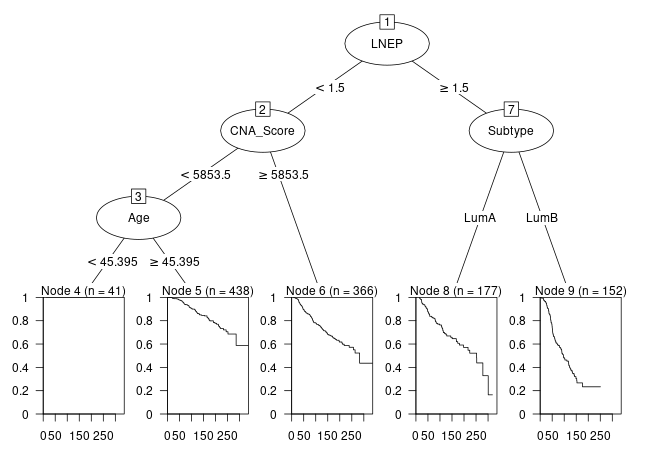
\includegraphics[width=0.75\textwidth]{../figures/Appendices/Appendix_A/LuminalAB_Rpart_DSS_Score.png}
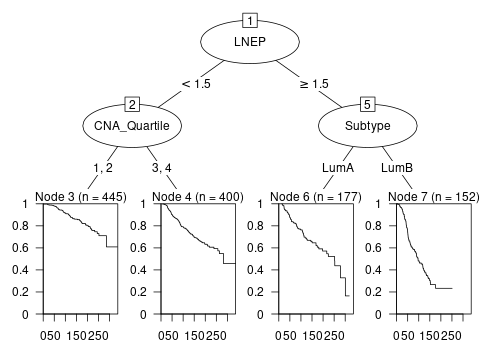
\includegraphics[width=0.75\textwidth]{../figures/Appendices/Appendix_A/LuminalAB_Rpart_DSS_Quart.png}
\caption[Recursive partitioning survival trees, fitted using the rpart algorithm, for disease-specific survival using clinical variables and CNA Score/Quartile as candidate predictors.]{Recursive partitioning survival trees, fitted using the rpart algorithm, for disease-specific survival using clinical variables and CNA Score and CNA Quartile as candidate predictors.}
\label{fig:LumAB_Trees_Quart_Rpart}
\end{figure}

\section*{Appendix B}
\renewcommand{\thefigure}{B\arabic{figure}}
\renewcommand{\thetable}{B\arabic{table}}
\setcounter{figure}{0}
\setcounter{table}{0}

\phantomsection
\addcontentsline{toc}{section}{Appendix B}

\markboth{\MakeUppercase{APPENDIX B}}{\MakeUppercase{APPENDIX B}}

Appendix B contains the rpart and ctree survival trees for OS outcomes. These survival trees are fitted under a number of scenarios (1) including PAM50 and IntClust only, (2) including Global CNA metrics and PAM50 or IntClust, (3) including Global CNA metrics, PAM50 subtype or IntClust, and a selection of clinical variables, (4) including Chromosome arm CNA metrics and PAM50 or IntClust, and (5) including Chromosome arm CNA metrics, PAM50 subtype or IntClust, and a selection of clinical variables. 

% OS using PAM50 Subtype/IntClust as candidate predictor
\captionsetup[subfigure]{font={normalfont,small}, skip=1pt, margin=-0.0cm, singlelinecheck=false}

\begin{figure}[!htbp]
\centering

\begin{minipage}{.44\textwidth}
\begin{subfigure}{\textwidth}
\subcaption{}
\includegraphics[width=\linewidth, height = 5.7cm]{../figures/Appendices/Appendix_B/Ind_Partykit_Survival_Score_OS_PAM50.png}
\end{subfigure}\par
\end{minipage}
\begin{minipage}{.55\textwidth}
\begin{subfigure}{\textwidth}
\subcaption{}
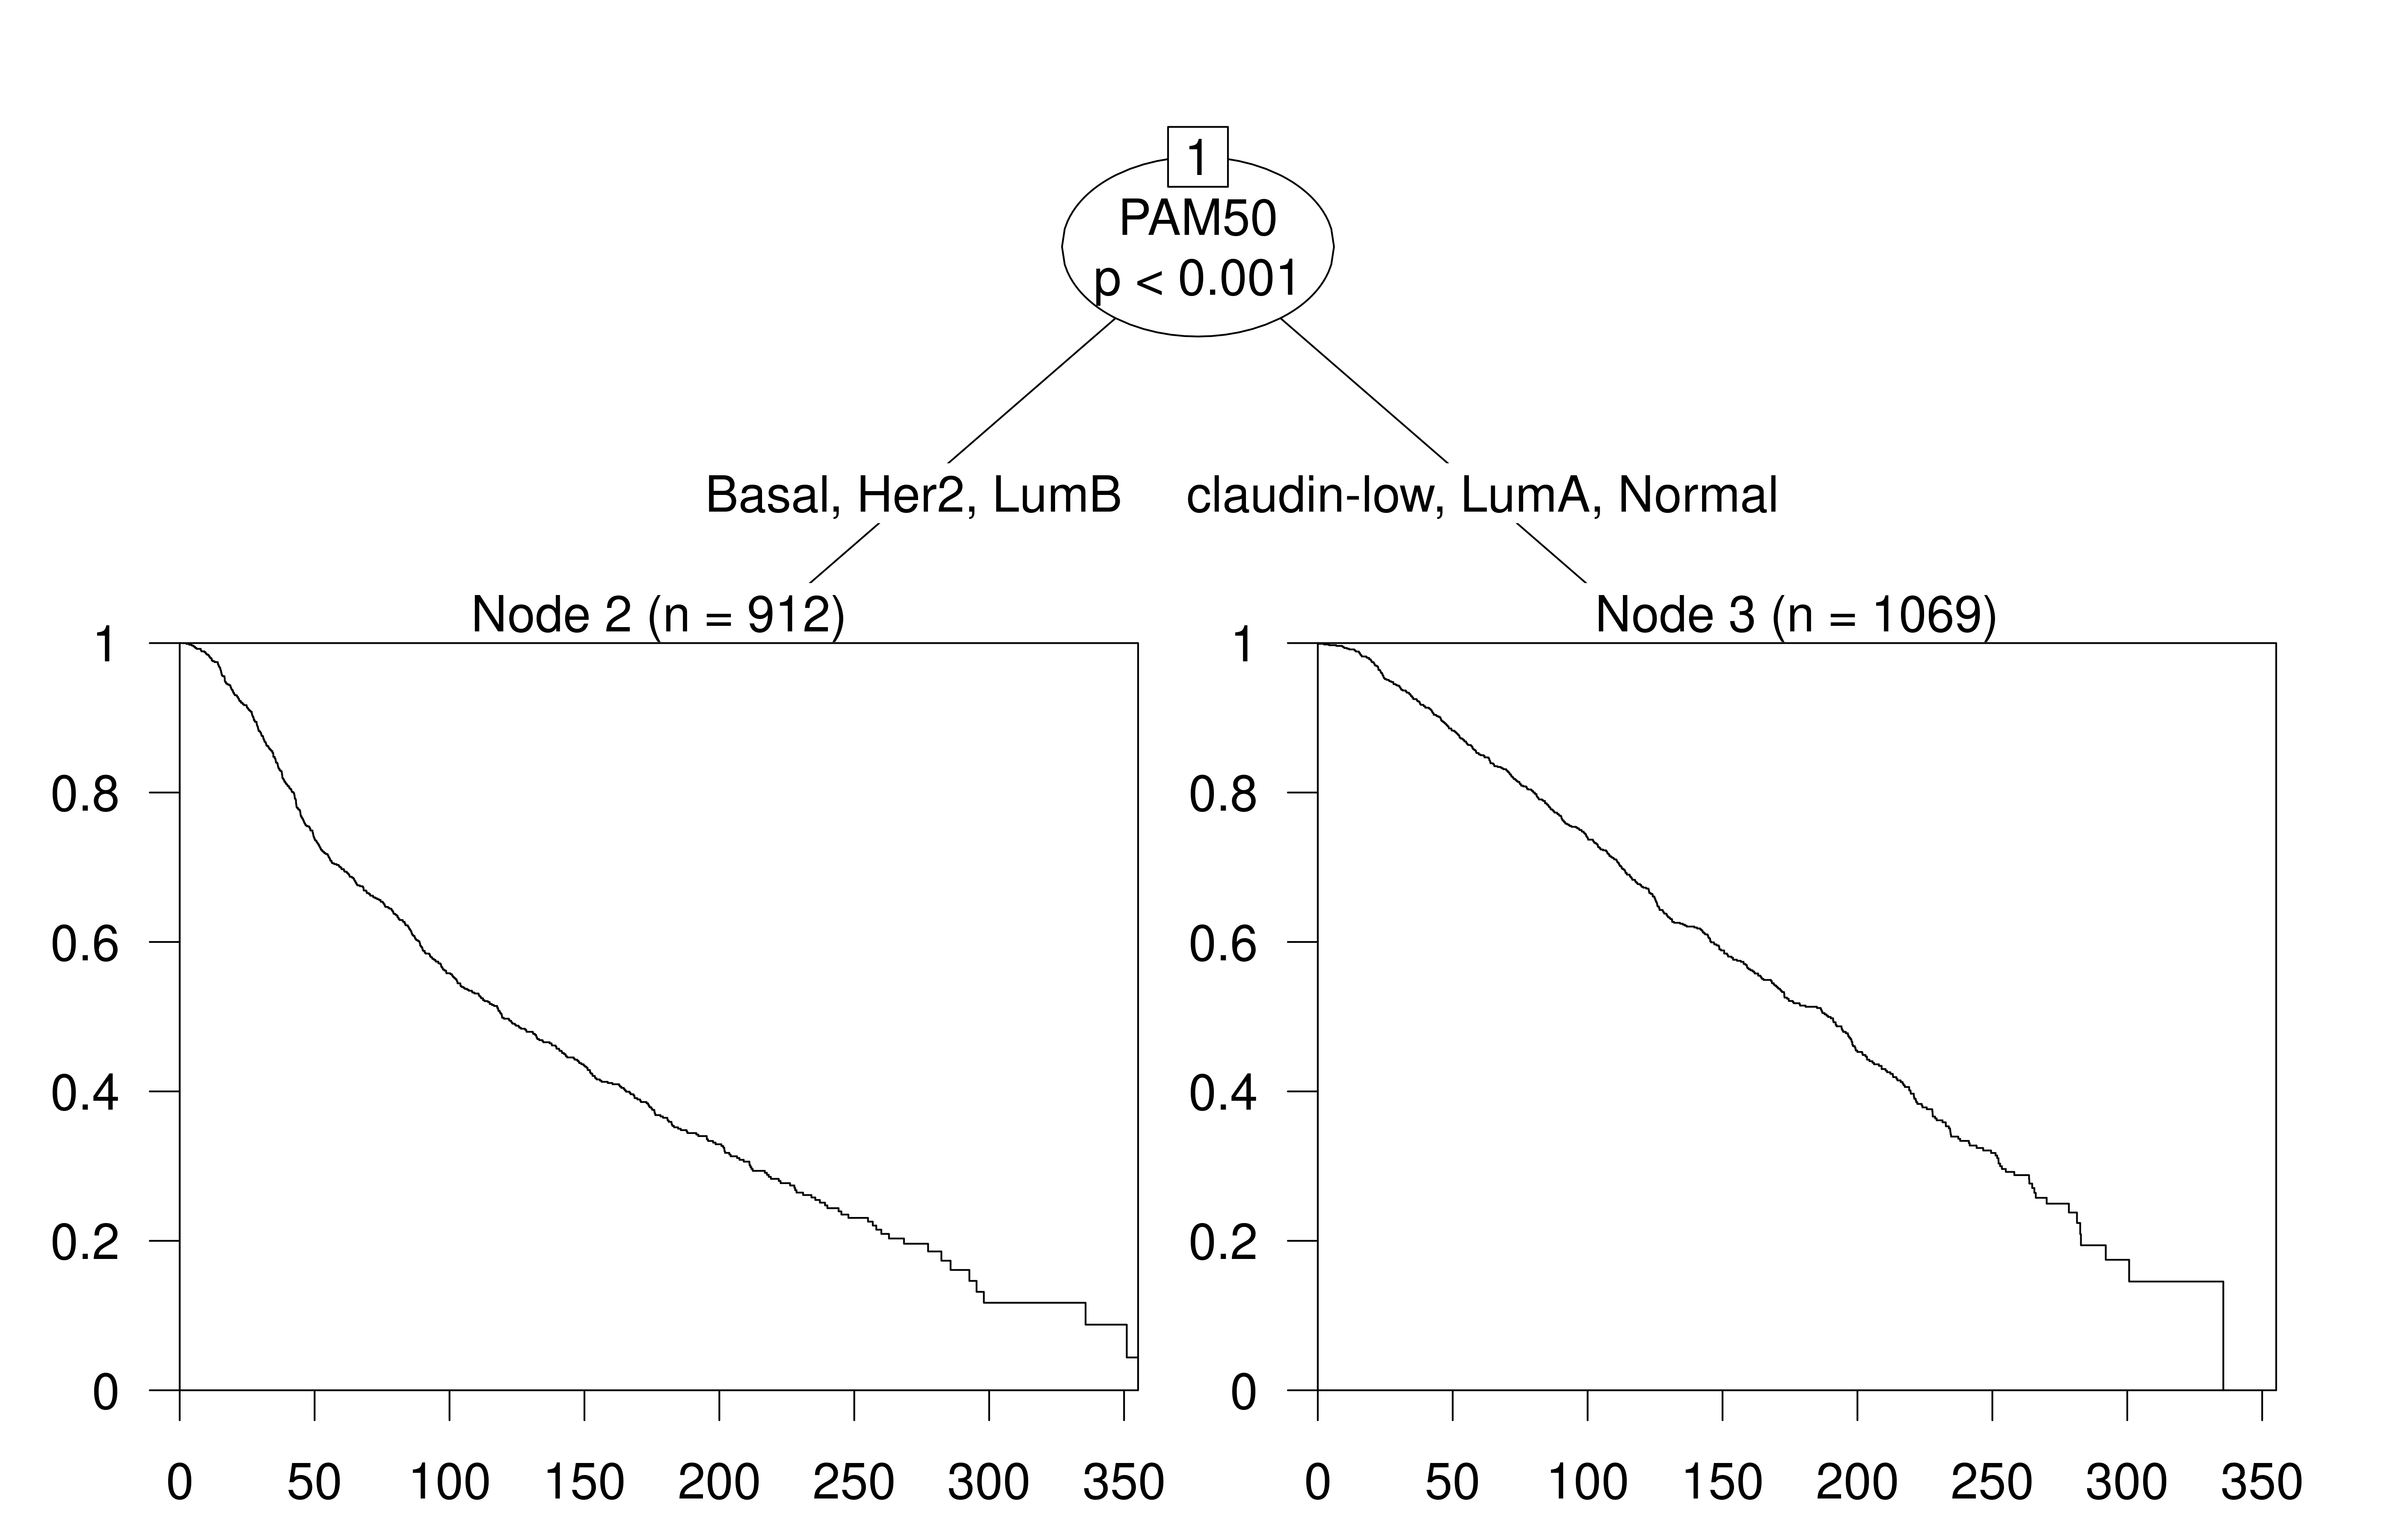
\includegraphics[width=\linewidth, height = 5.7cm]{../figures/Appendices/Appendix_B/Ind_Ctree_Survival_Score_OS_PAM50.png}
\end{subfigure}\par
\end{minipage}

\caption[Recursive partitioning survival trees for overall survival using PAM50 Subtype as a candidate predictor.]{Recursive partitioning survival trees for overall survival using PAM50 Subtype as a candidate predictor. (A) Trees fitted using the rpart algorithm and (B) trees fitted using the ctree algorithm.}
\end{figure}

\begin{figure}[!htbp]
\centering

\begin{minipage}{.44\textwidth}
\begin{subfigure}{\textwidth}
\subcaption{}
\includegraphics[width=\linewidth, height = 5.7cm]{../figures/Appendices/Appendix_B/Ind_Partykit_Survival_Score_OS_INTCLUST.png}
\end{subfigure}\par
\end{minipage}
\begin{minipage}{.55\textwidth}
\begin{subfigure}{\textwidth}
\subcaption{}
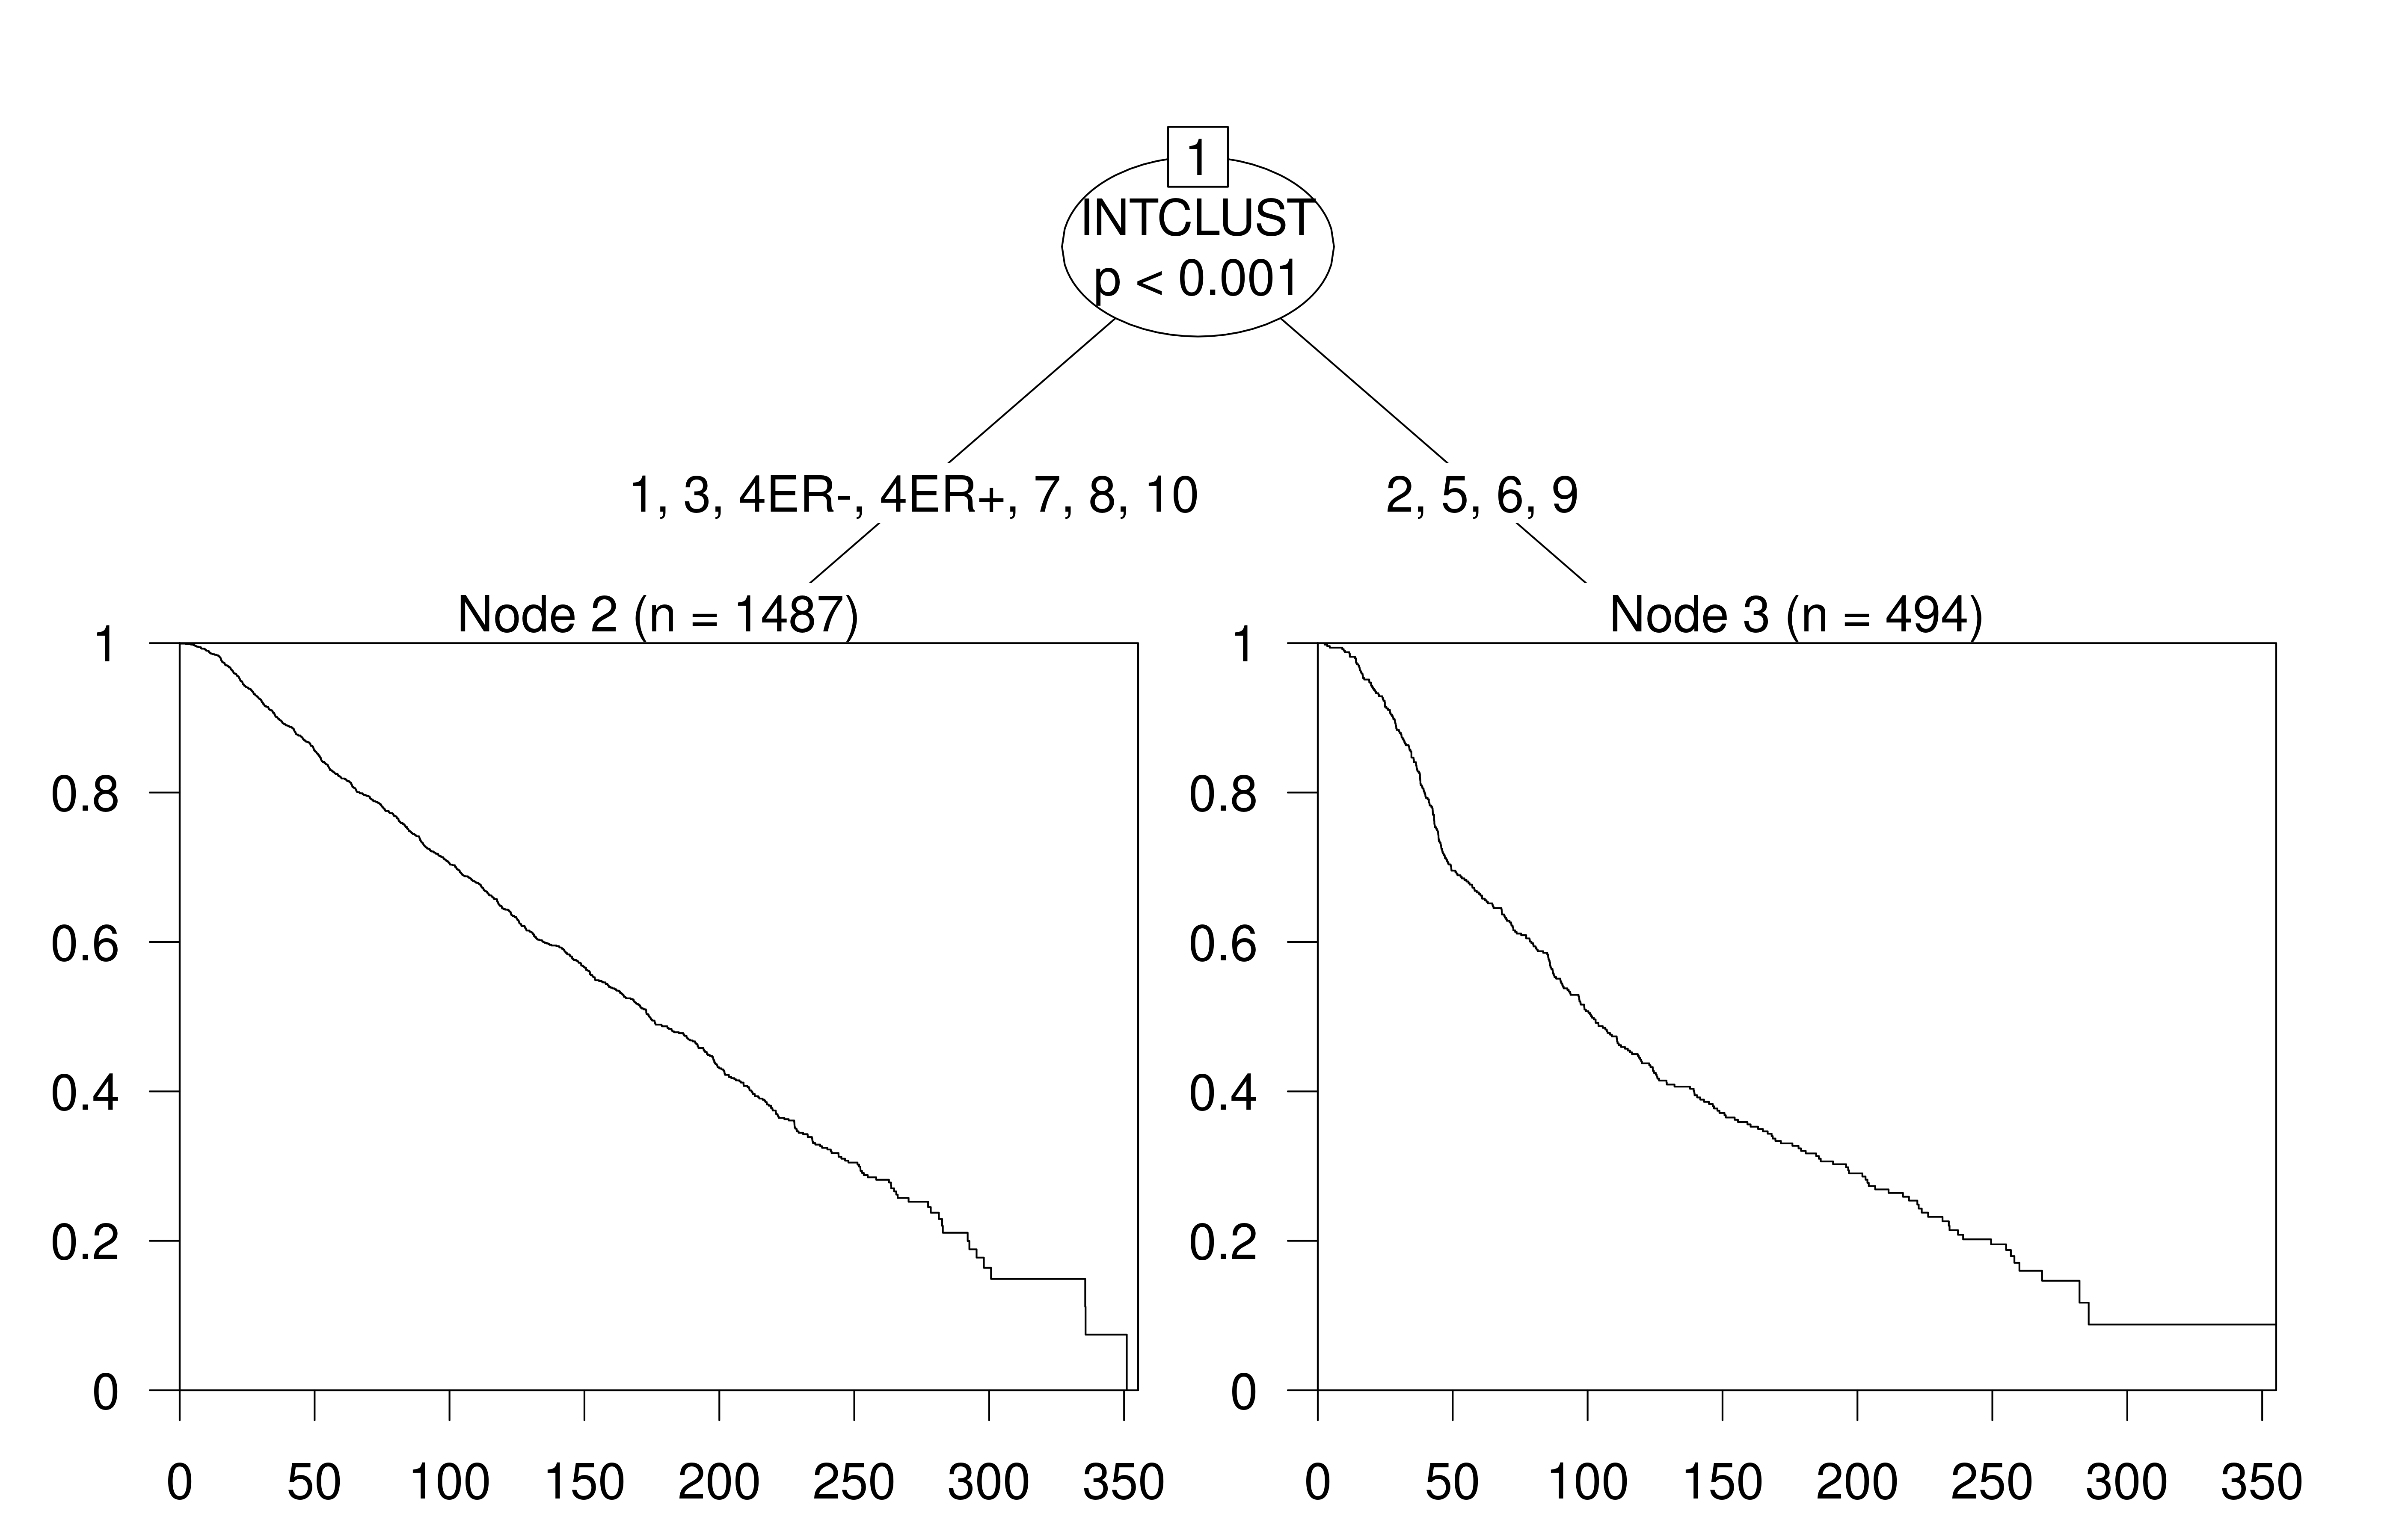
\includegraphics[width=\linewidth, height = 5.7cm]{../figures/Appendices/Appendix_B/Ind_Ctree_Survival_Score_OS_INTCLUST.png}
\end{subfigure}\par
\end{minipage}

\caption[Recursive partitioning survival trees for overall survival using Integrative Cluster as a candidate predictor.]{Recursive partitioning survival trees for overall survival using Integrative Cluster as a candidate predictor. (A) Trees fitted using the rpart algorithm and (B) trees fitted using the ctree algorithm.}
\end{figure}

% Global CNA metrics 
% OS using PAM50 Subtype and the 6 CNA Score metrics as candidate predictor

\begin{figure}[!htb]
\centering

\vspace{0.5cm}

\begin{subfigure}{\textwidth}
\subcaption{}
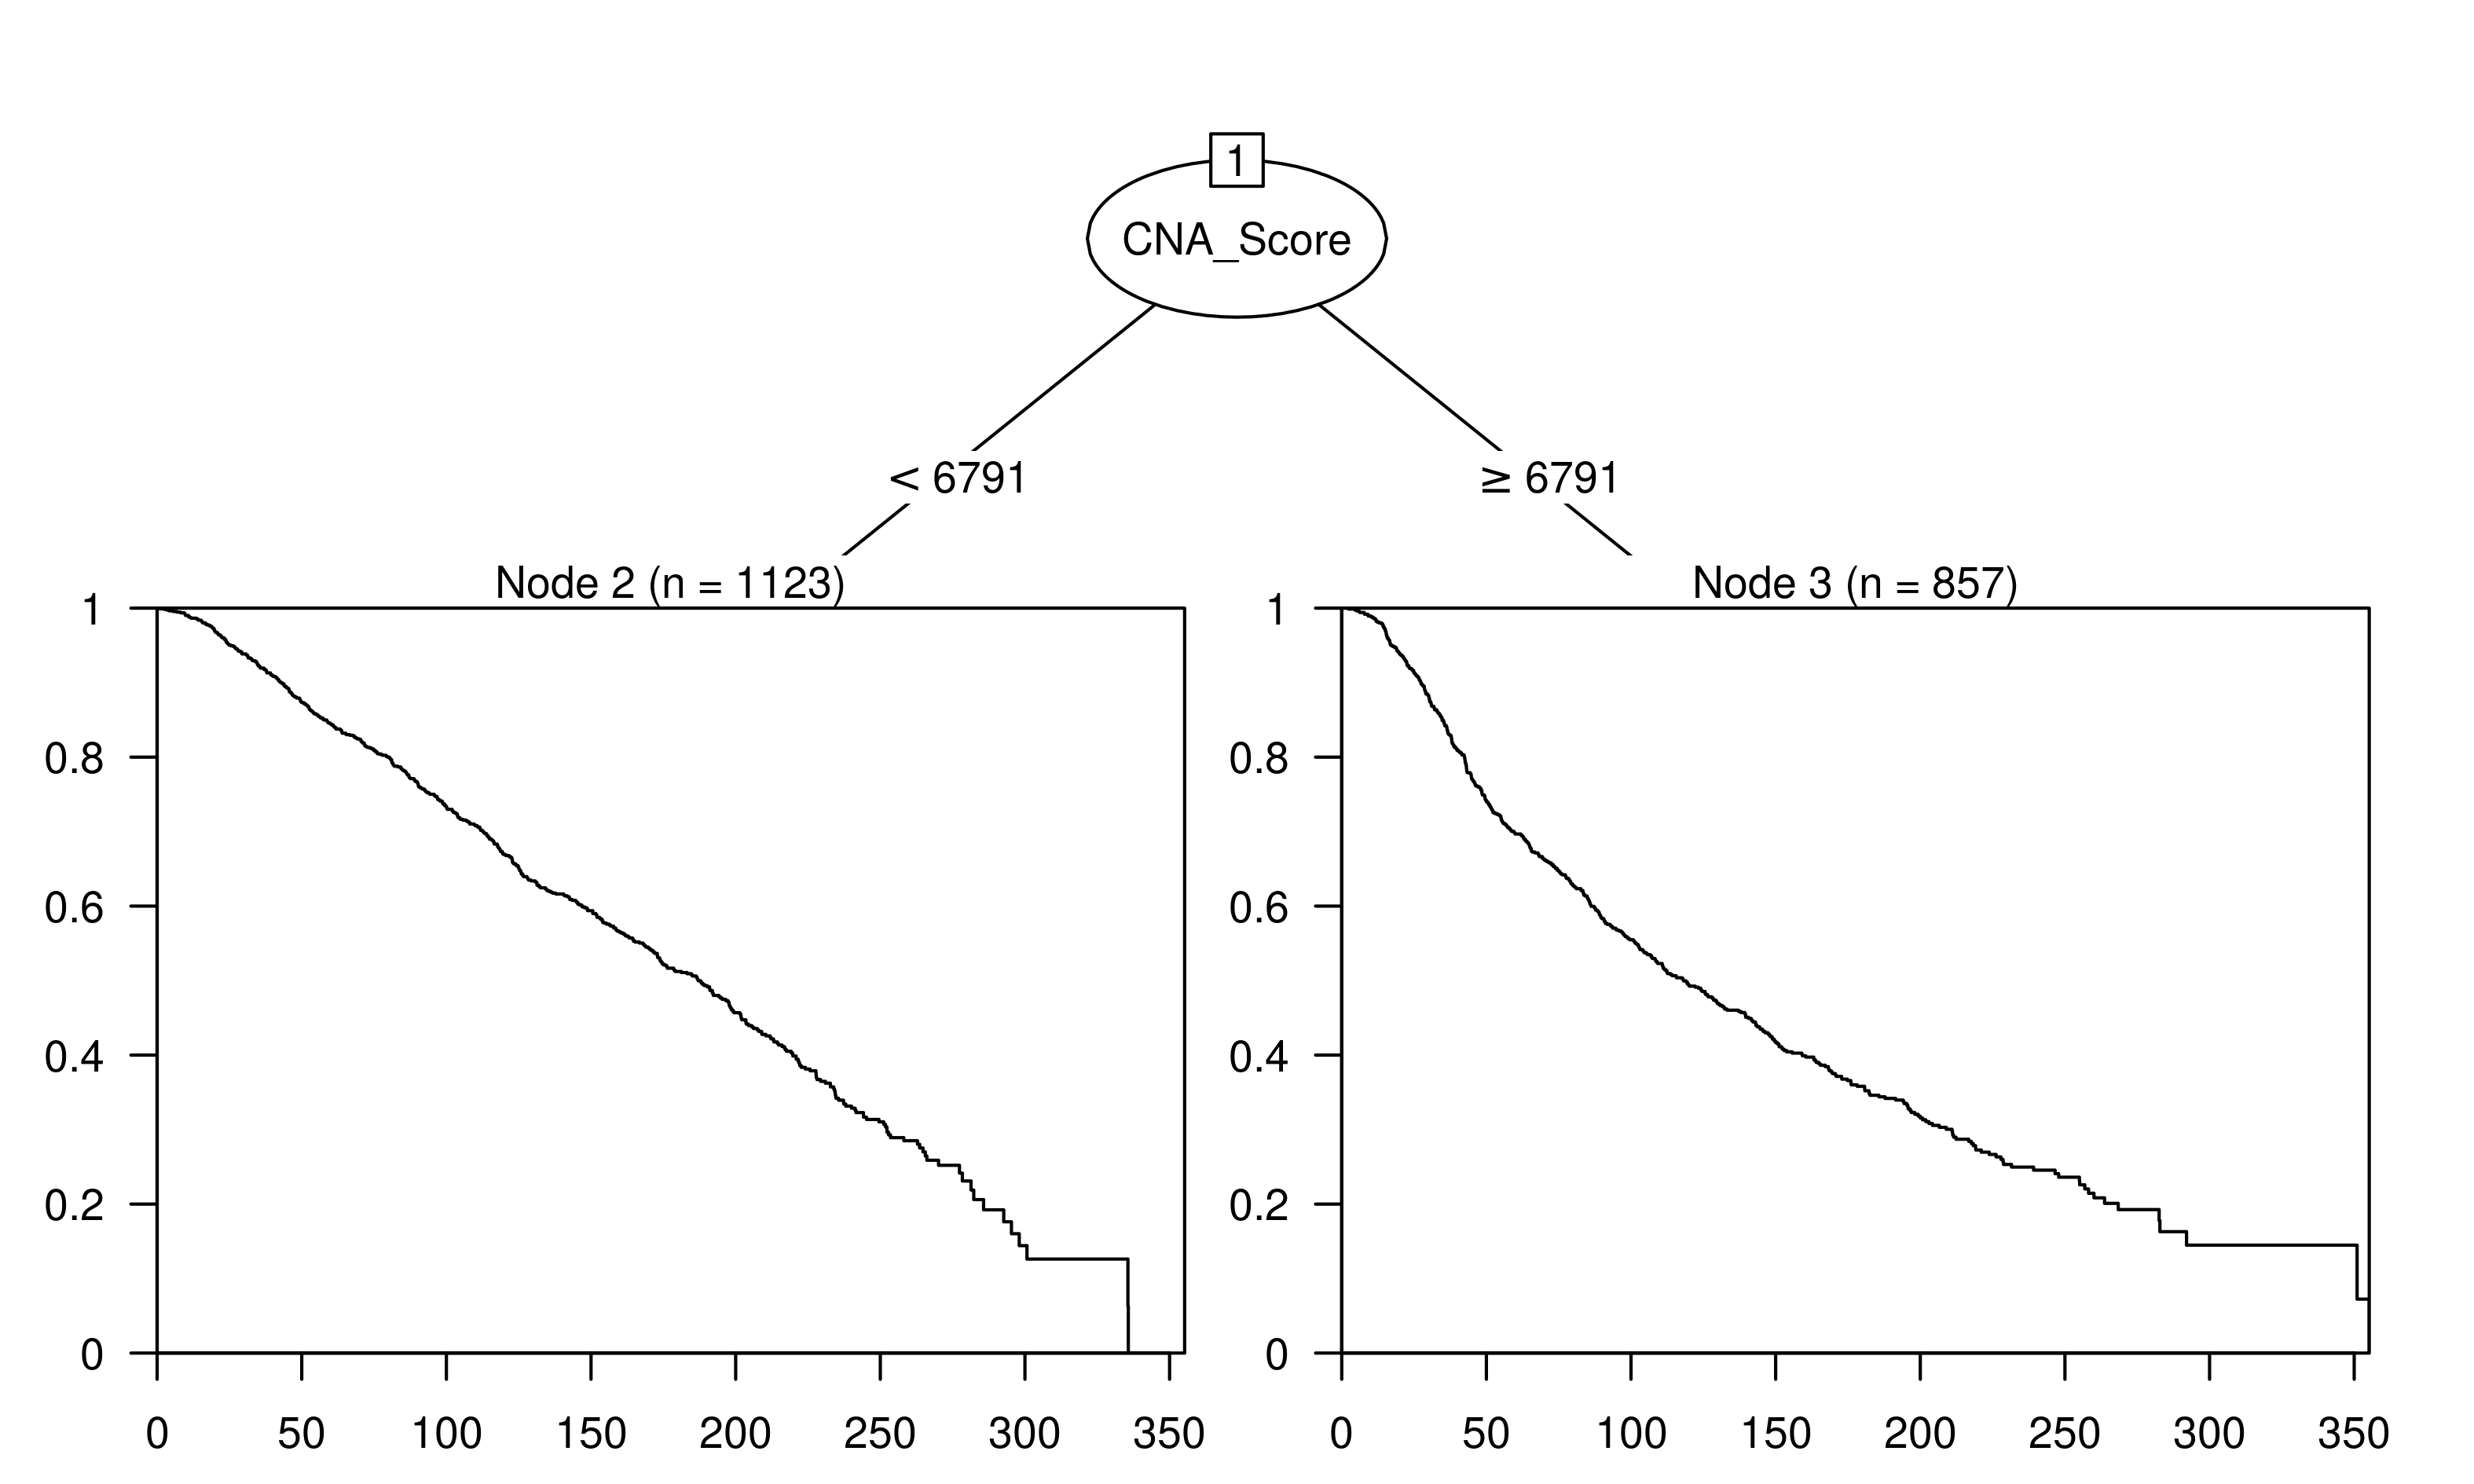
\includegraphics[width=1\textwidth]{../figures/Appendices/Appendix_B/PartyKit_Survival_Score_OS_PAM50.png}
\end{subfigure}

\vspace{2cm}

\begin{subfigure}{\textwidth}
\subcaption{}
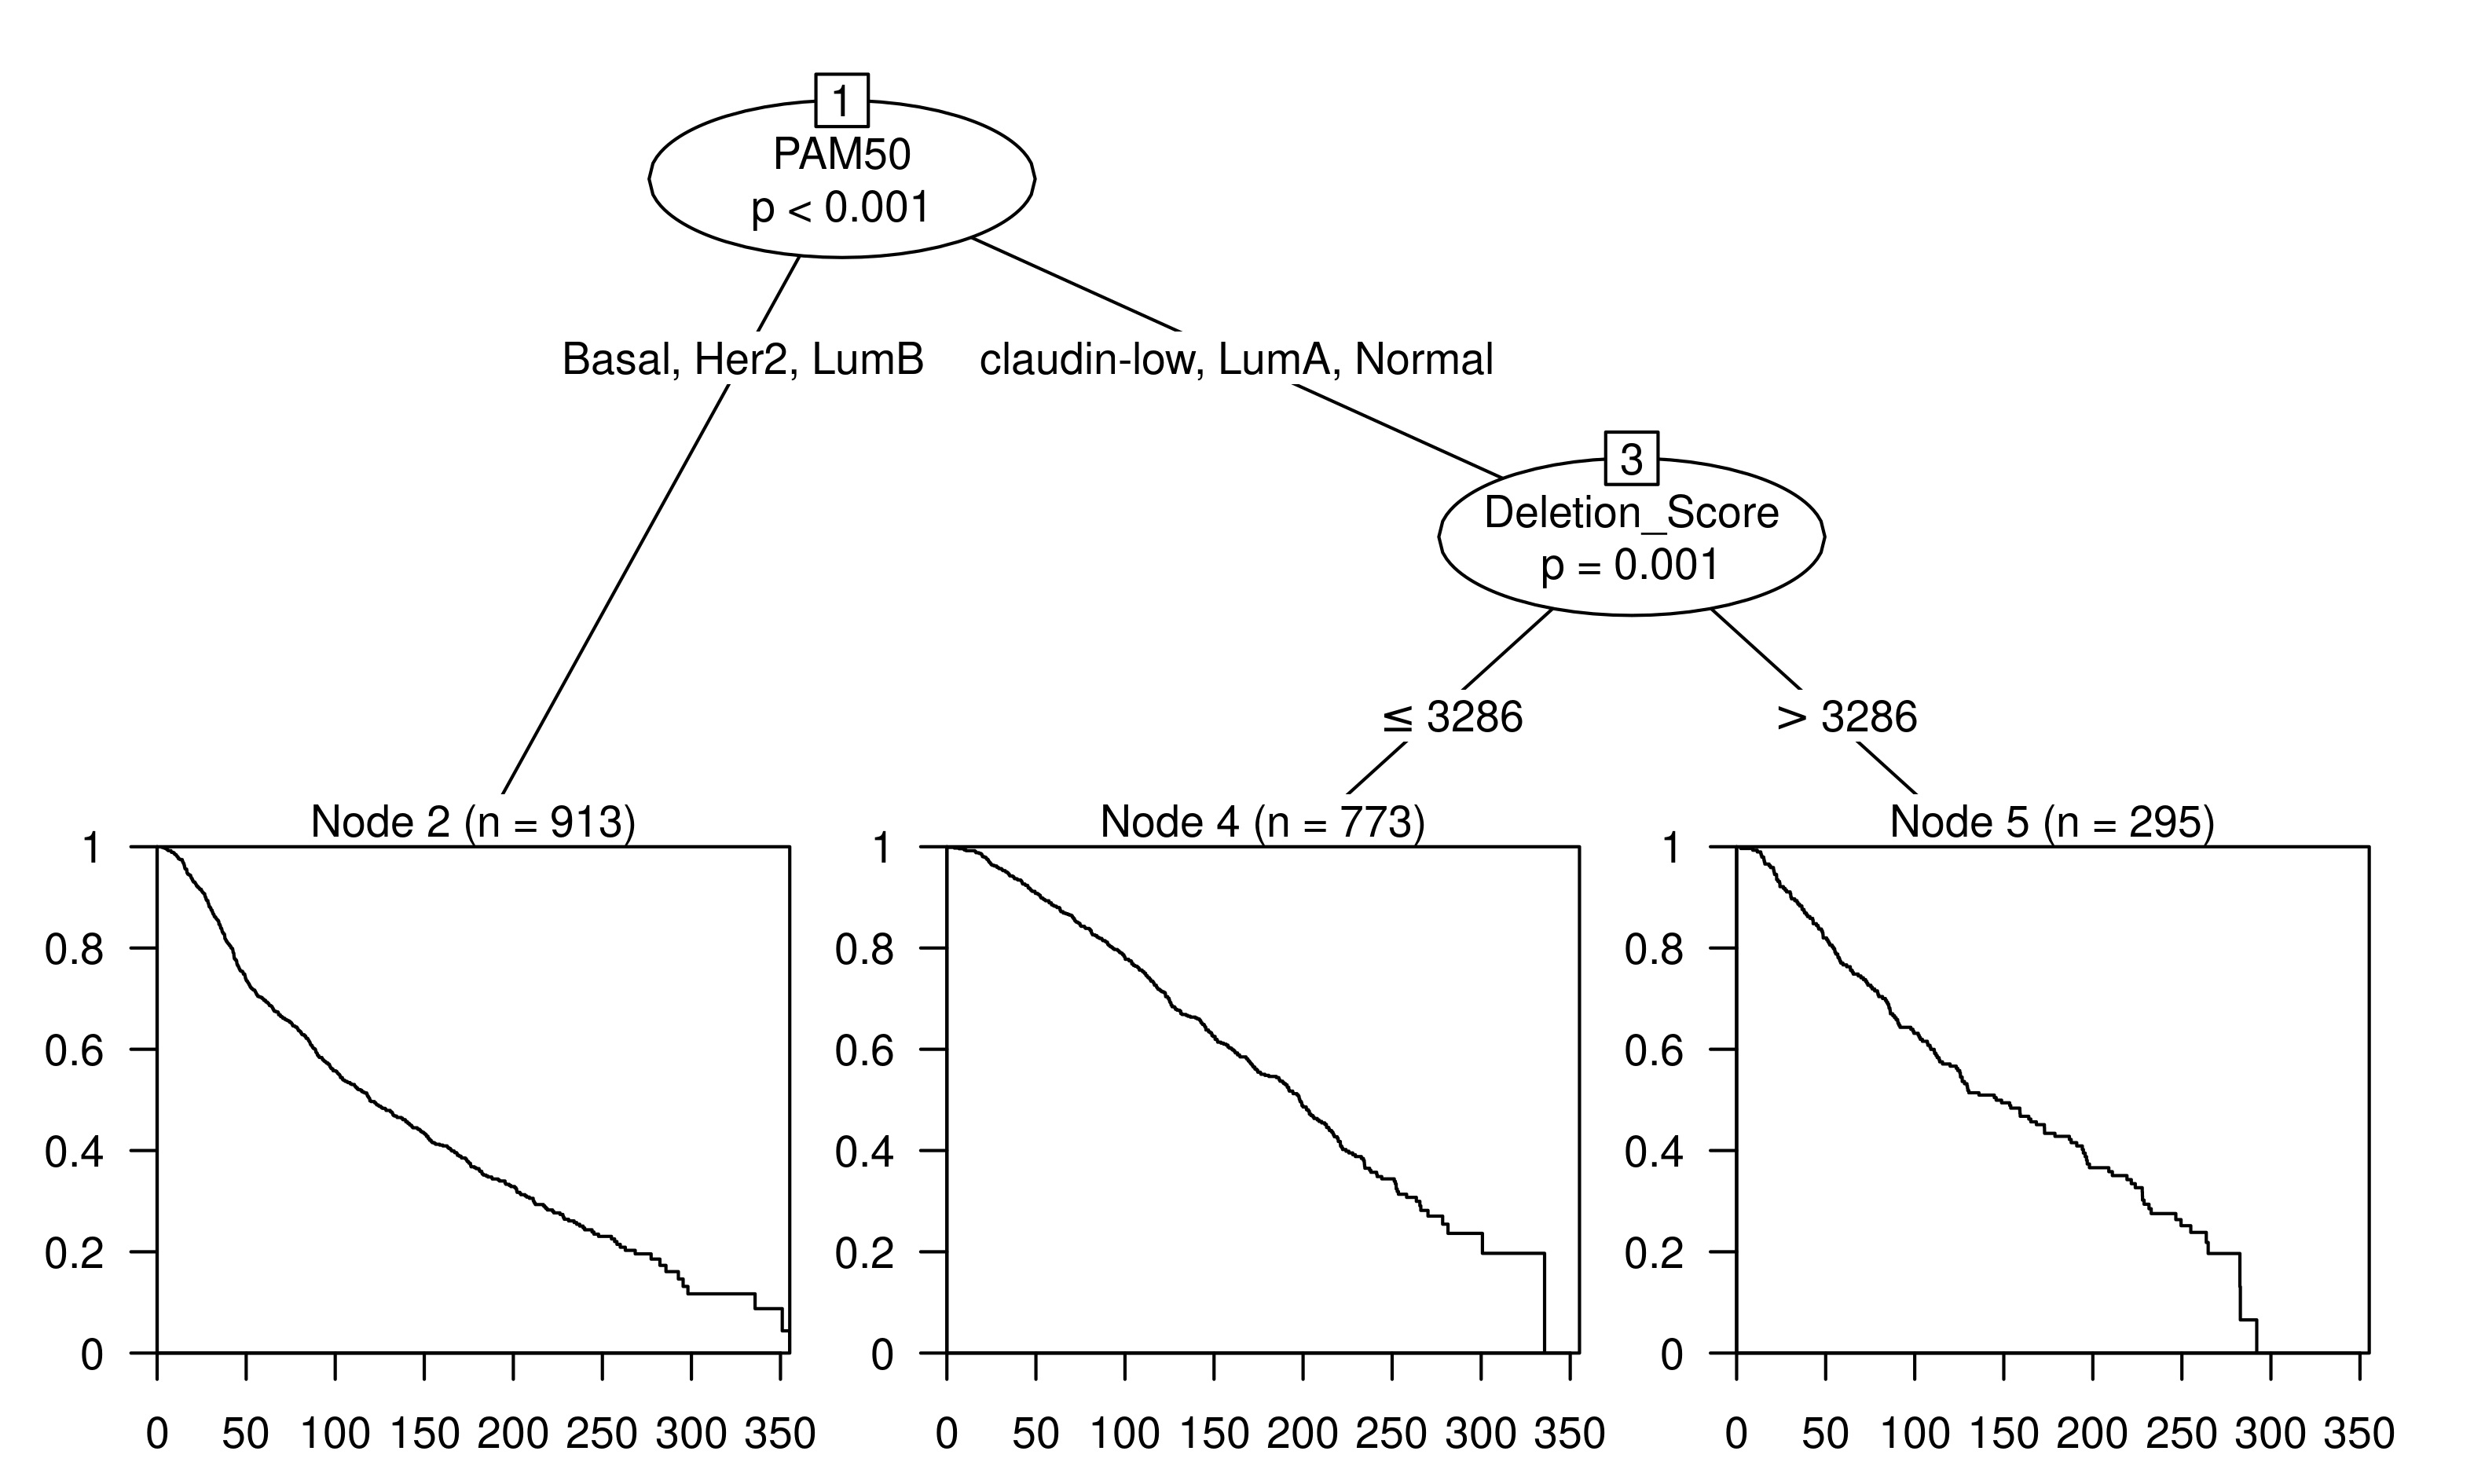
\includegraphics[width=1\textwidth]{../figures/Appendices/Appendix_B/Ctree_Survival_Score_OS_PAM50.png}
\end{subfigure}

\vspace{0.5cm}

\caption[Recursive partitioning survival trees for overall survival using PAM50 and the 6 CNA Score metrics as candidate predictors.]{Recursive partitioning survival trees for overall survival using PAM50 and the six CNA Score metrics as candidate predictors. Trees fitted using the rpart algorithm are displayed on the top and trees fitted using the ctree algorithm are displayed on the bottom.}
\end{figure}

\begin{figure}[!htb]
\centering

\vspace{0.5cm}

\begin{subfigure}{\textwidth}
\subcaption{}
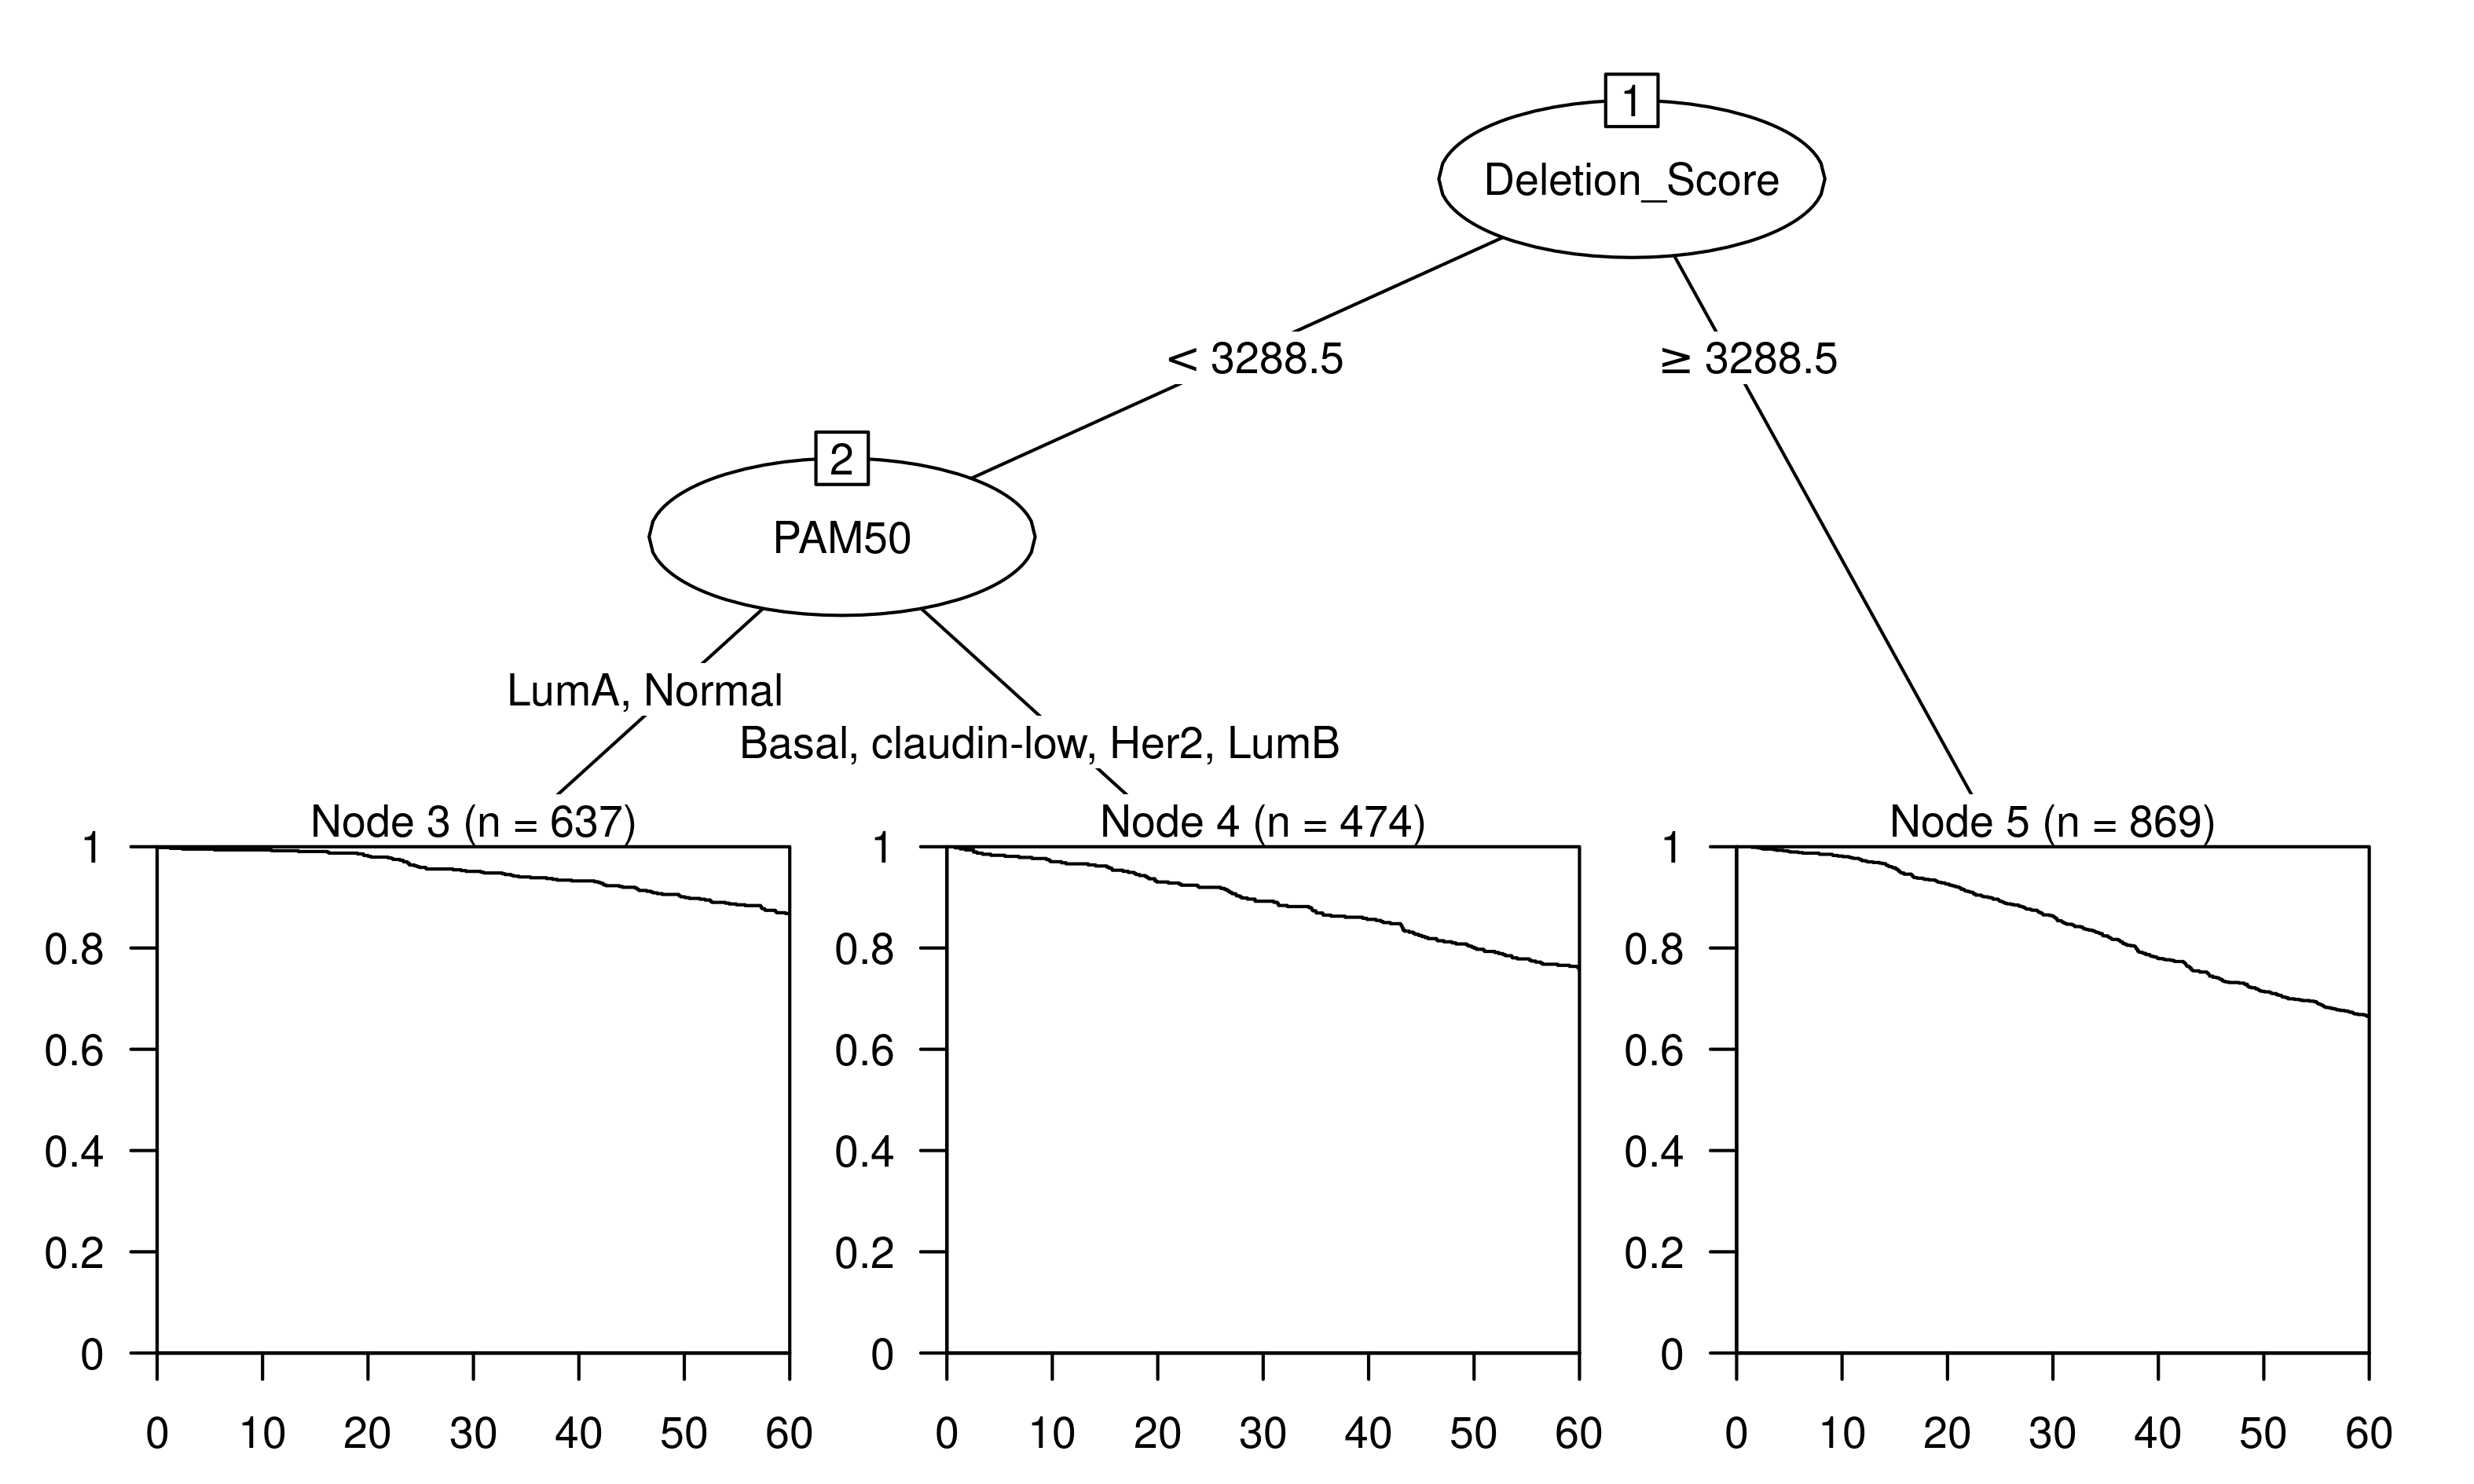
\includegraphics[width=1\textwidth]{../figures/Appendices/Appendix_B/PartyKit_Survival_Score_FiveYearOS_PAM50.png}
\end{subfigure}

\vspace{2cm}

\begin{subfigure}{\textwidth}
\subcaption{}
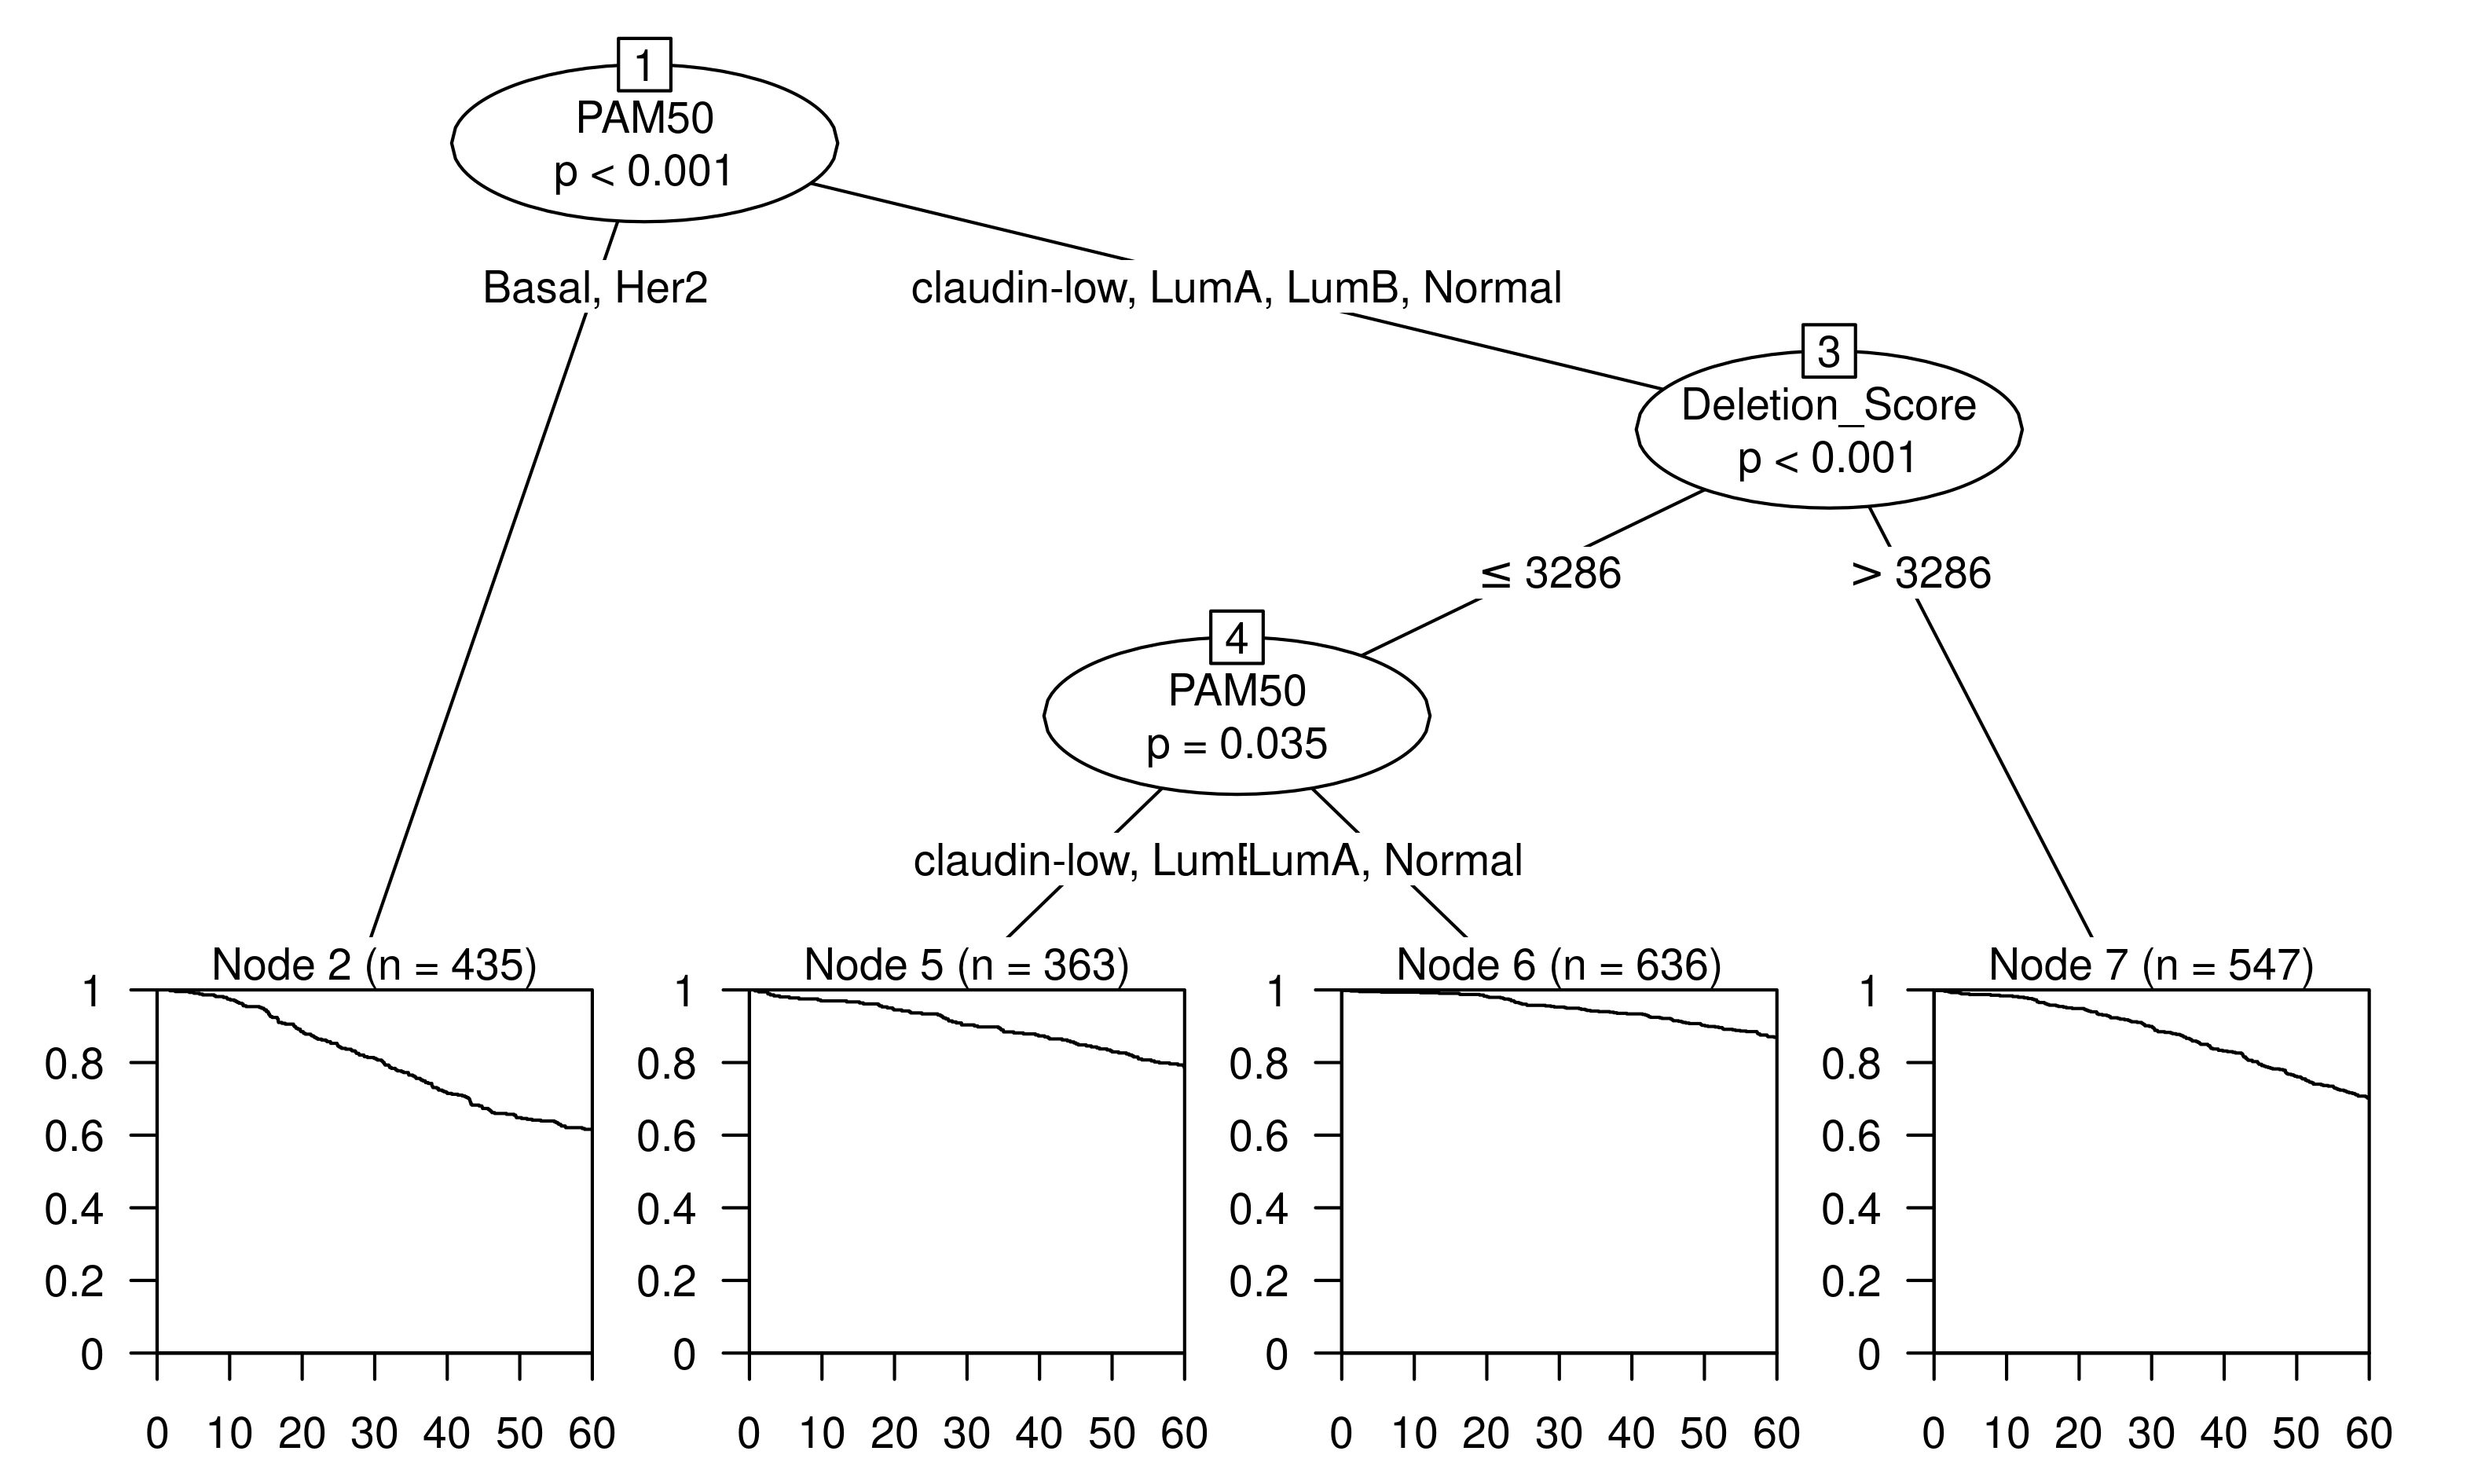
\includegraphics[width=1\textwidth]{../figures/Appendices/Appendix_B/Ctree_Survival_Score_FiveYearOS_PAM50.png}
\end{subfigure}

\vspace{0.5cm}

\caption[Recursive partitioning survival trees for five-year overall survival using PAM50 and the six CNA Score metrics as candidate predictors.]{Recursive partitioning survival trees for five-year overall survival using PAM50 and the six CNA Score metrics as candidate predictors. (A) Trees fitted using the rpart algorithm and (B) trees fitted using the ctree algorithm.}
\end{figure}

\begin{figure}[!htb]
\centering

\vspace{0.5cm}

\begin{subfigure}{\textwidth}
\subcaption{}
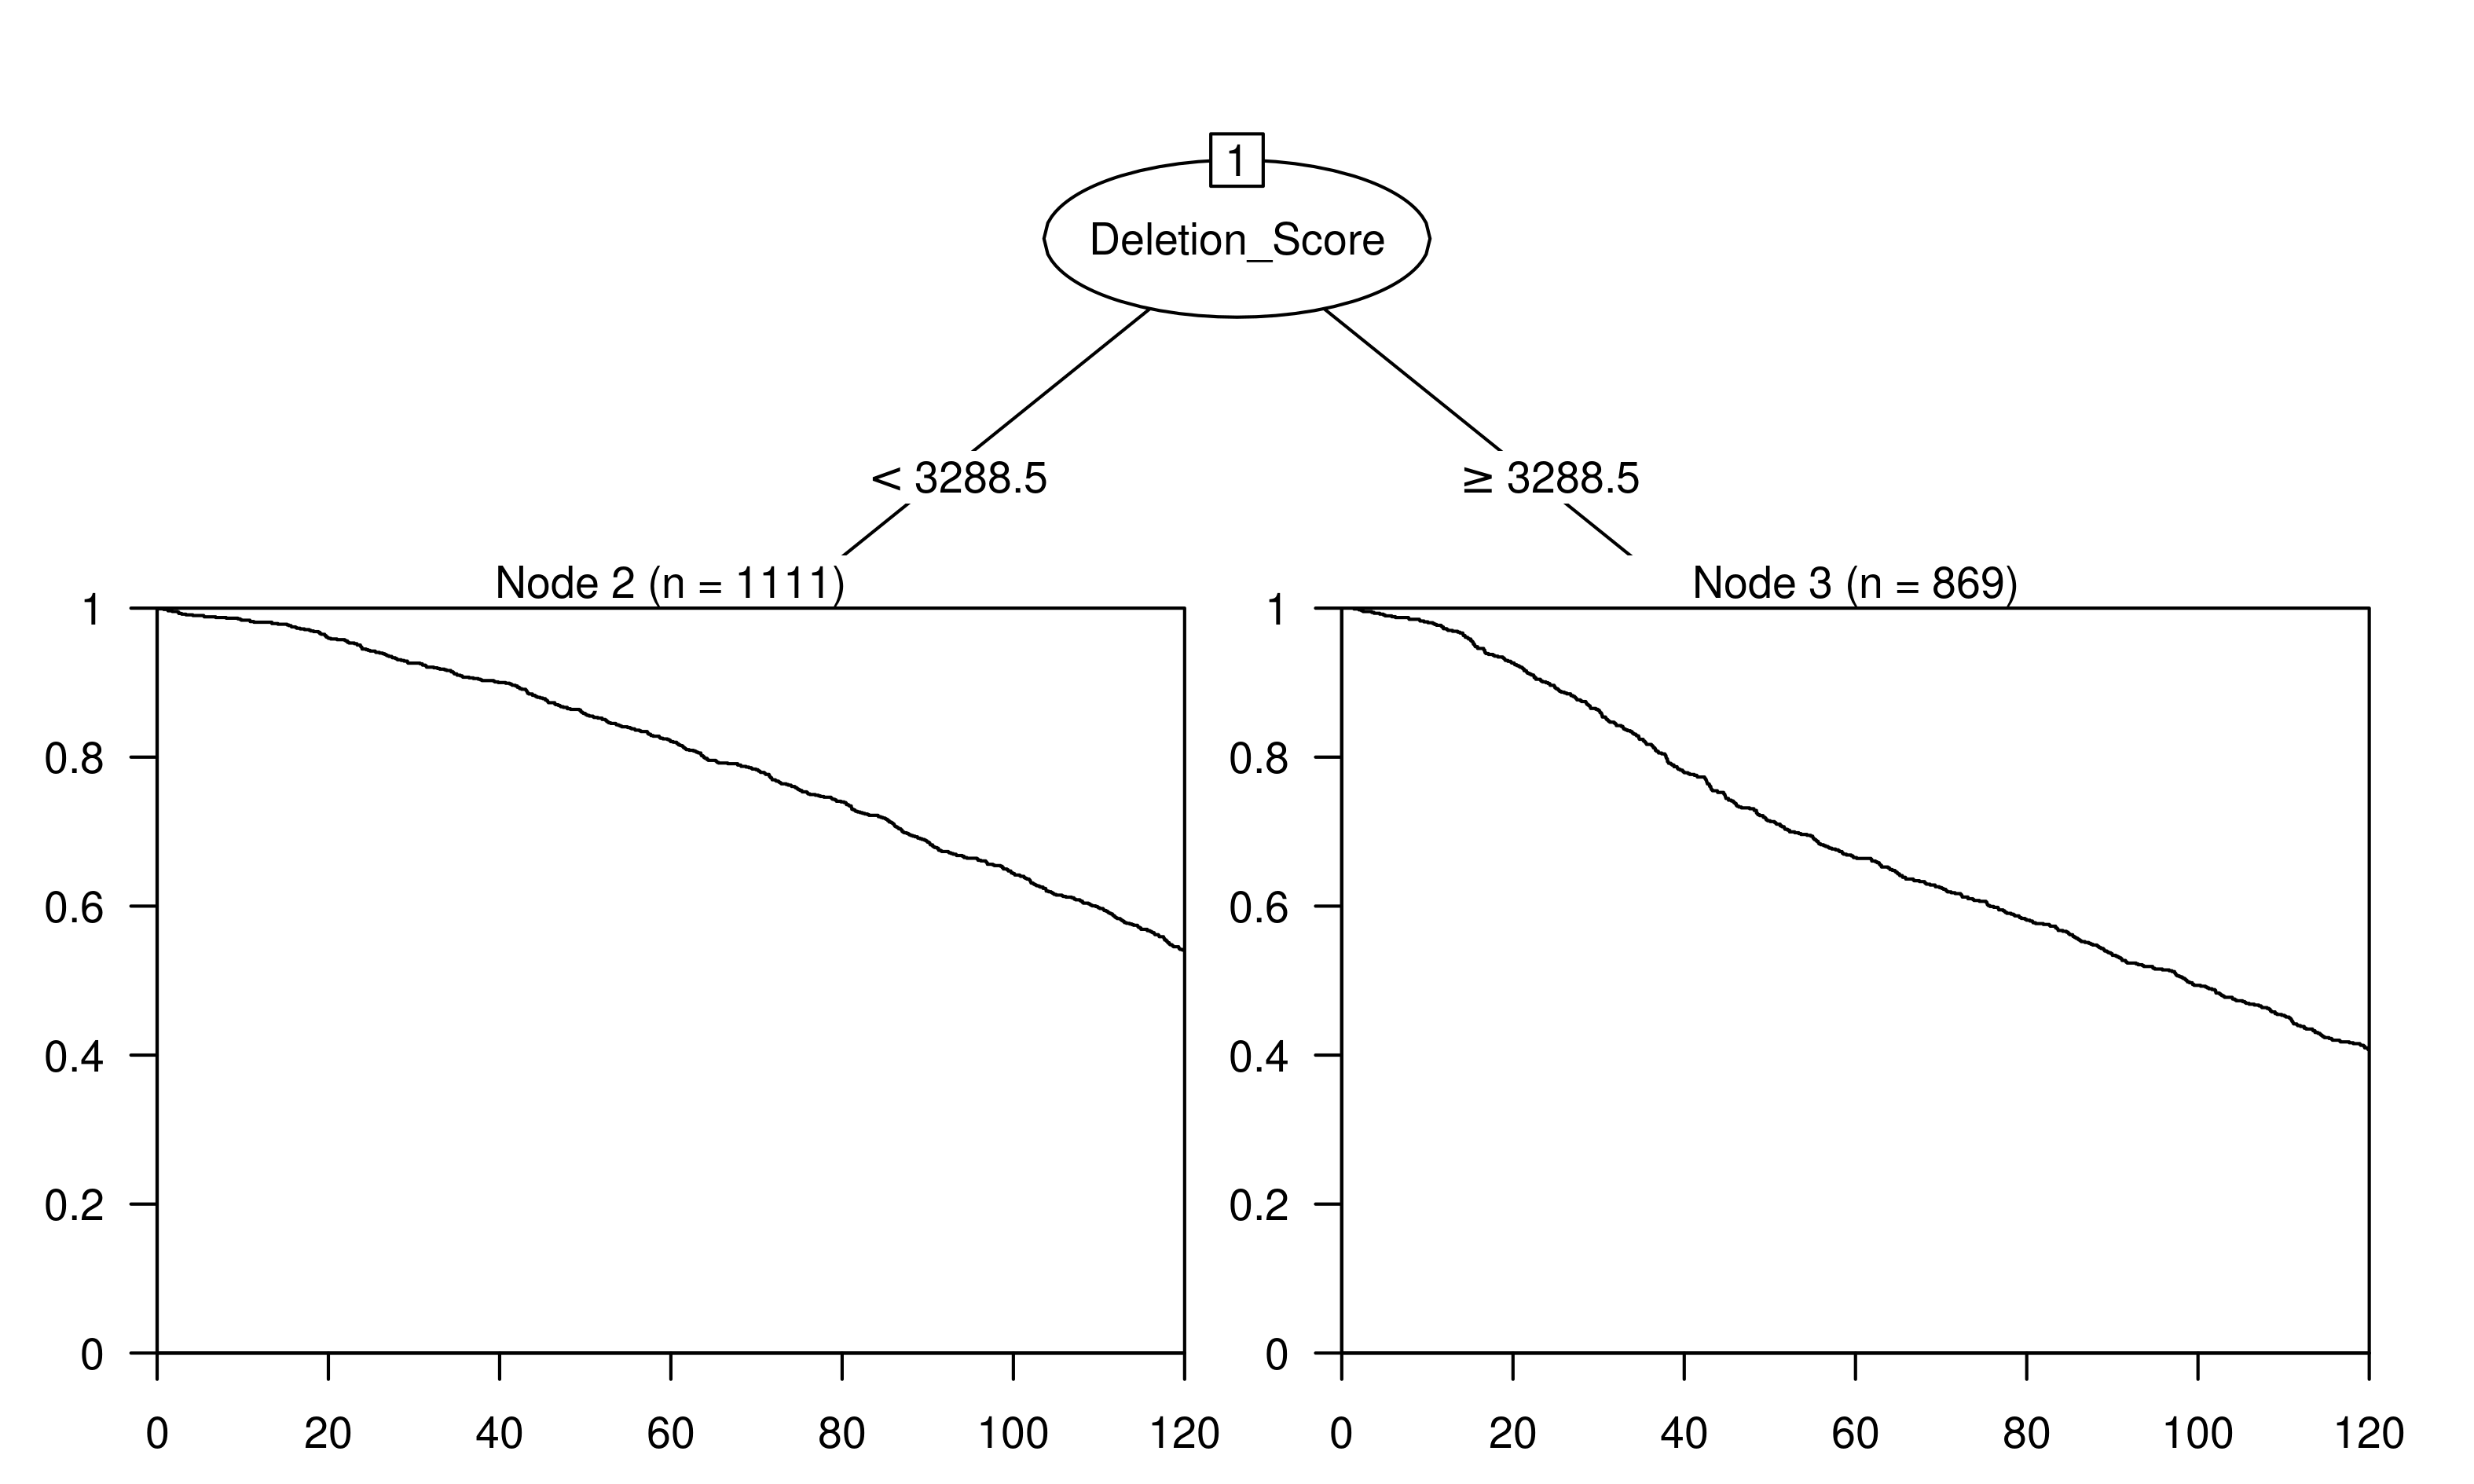
\includegraphics[width=1\textwidth]{../figures/Appendices/Appendix_B/PartyKit_Survival_Score_TenYearOS_PAM50.png}
\end{subfigure}

\vspace{2cm}

\begin{subfigure}{\textwidth}
\subcaption{}
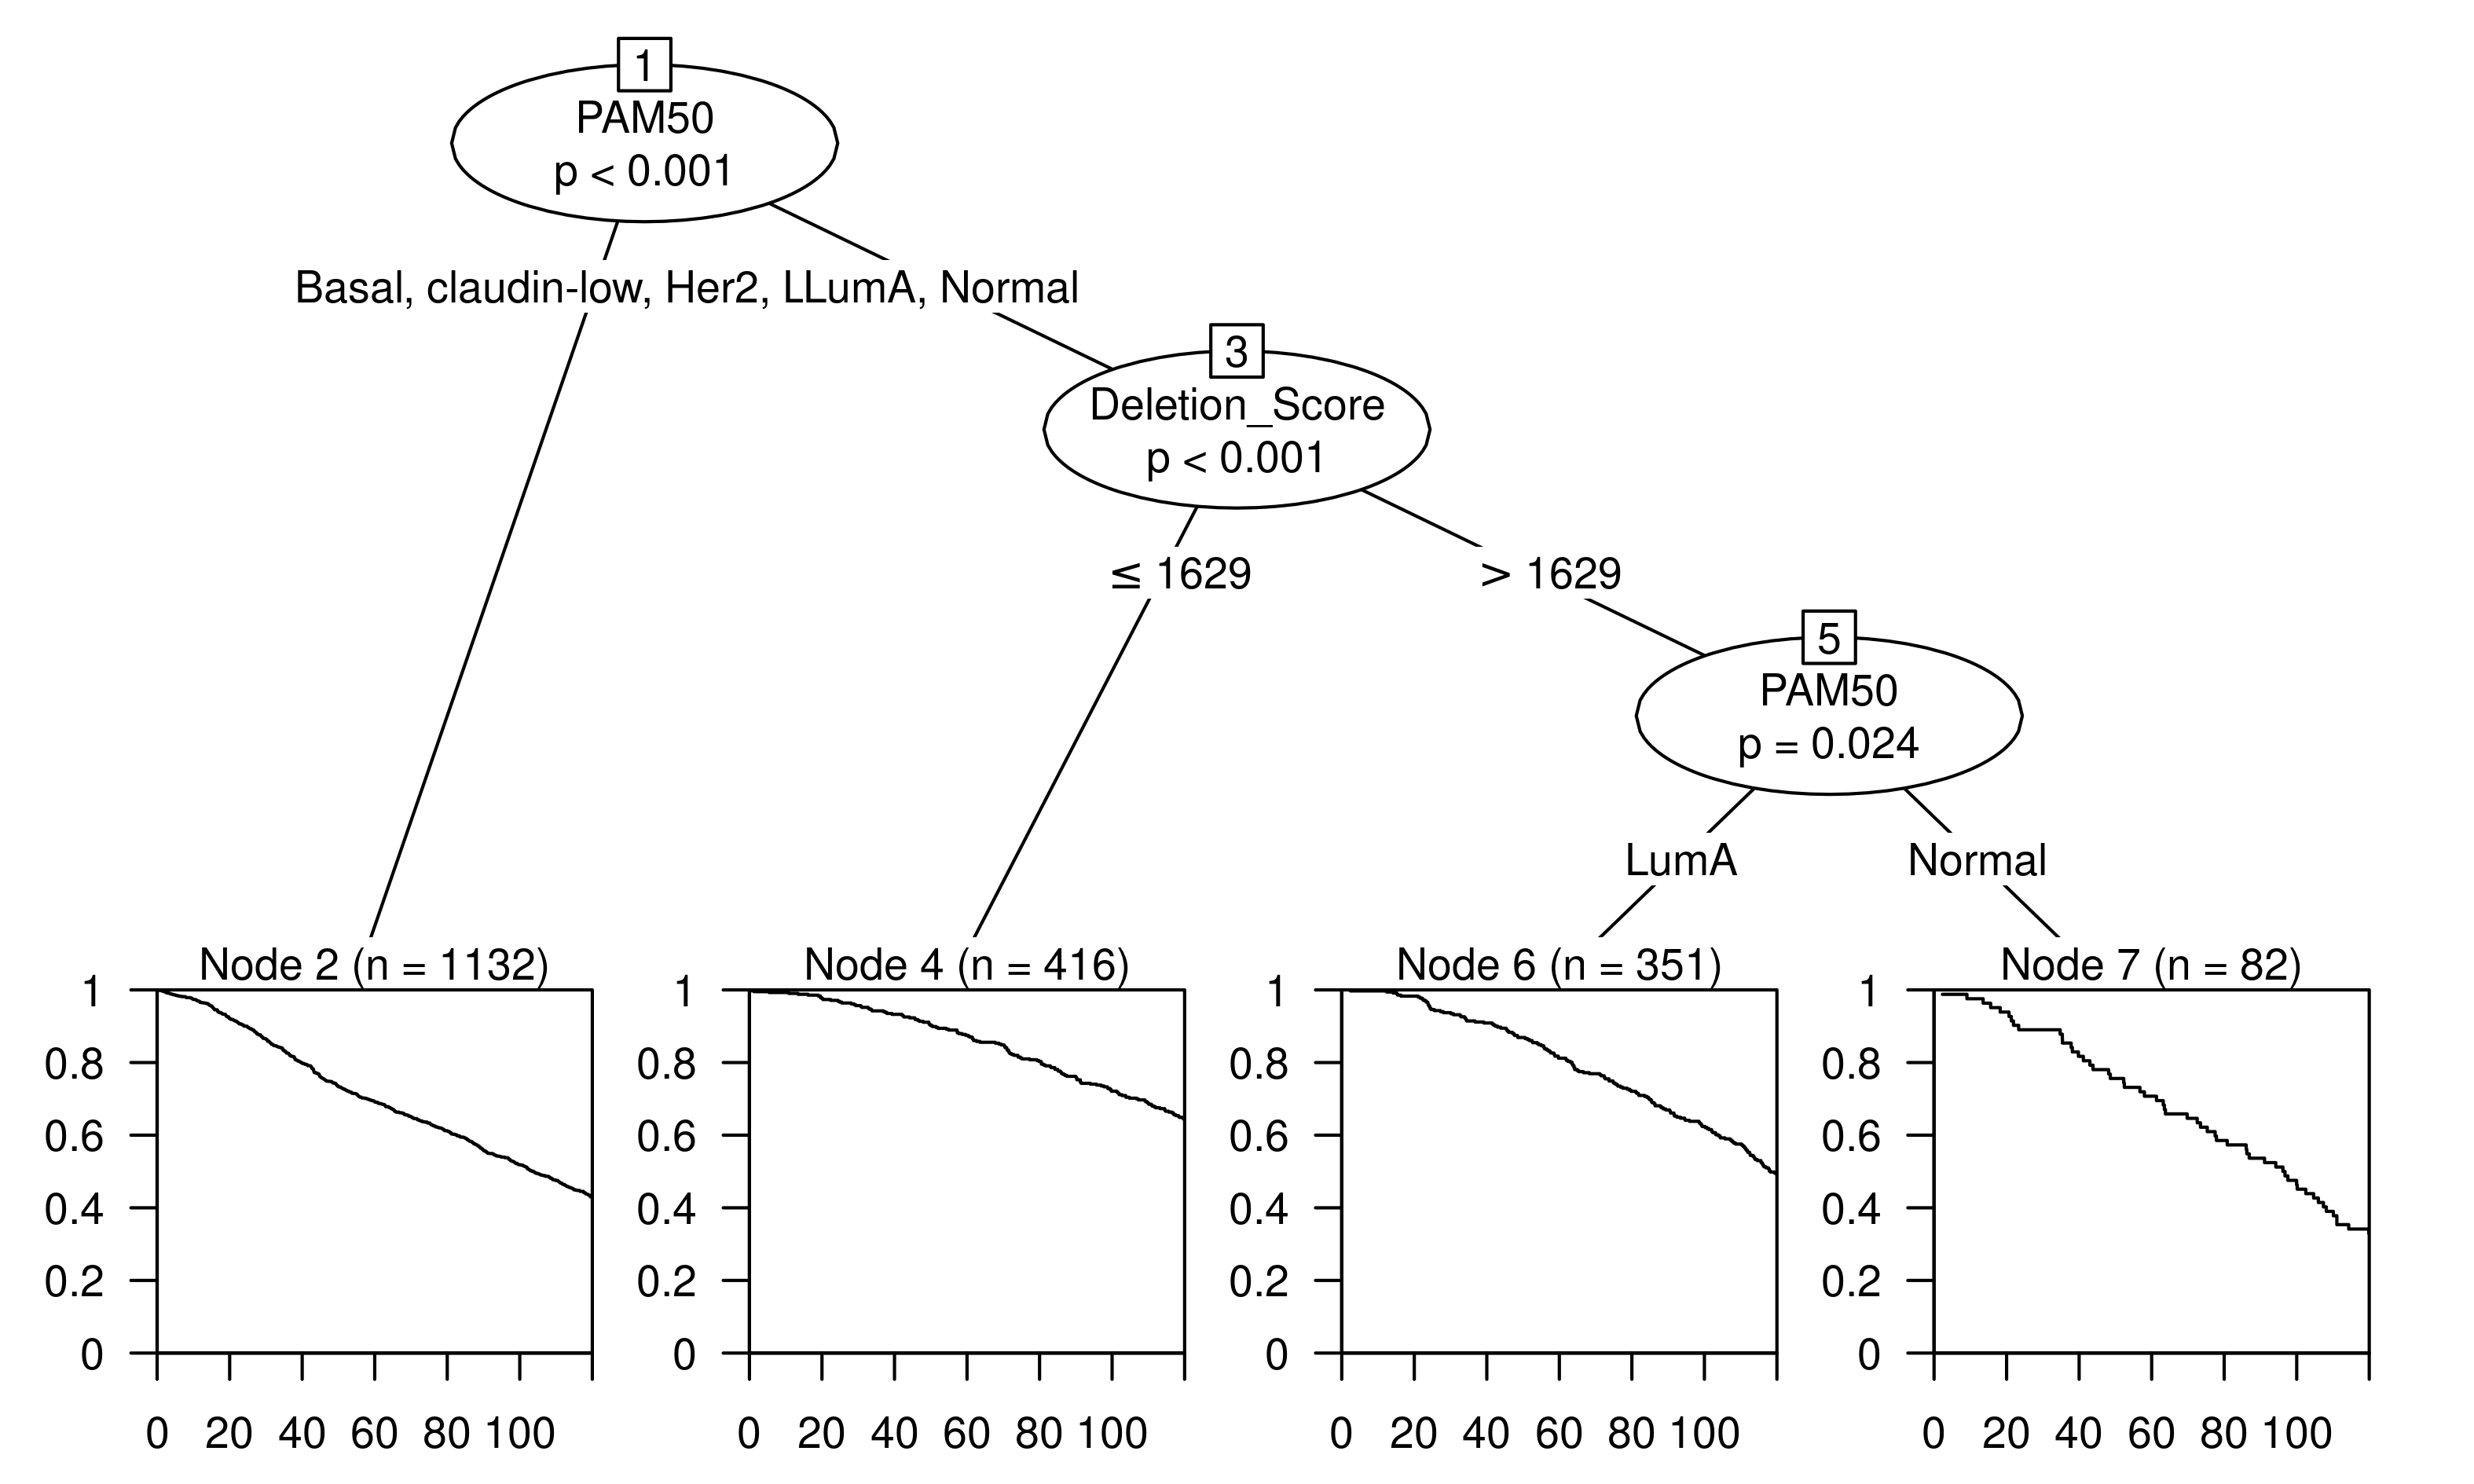
\includegraphics[width=1\textwidth]{../figures/Appendices/Appendix_B/Ctree_Survival_Score_TenYearOS_PAM50.png}
\end{subfigure}

\vspace{0.5cm}

\caption[Recursive partitioning survival trees for ten-year overall survival using PAM50 and the six CNA Score metrics as candidate predictors.]{Recursive partitioning survival trees for ten-year overall survival using PAM50 and the six CNA Score metrics as candidate predictors. (A) Trees fitted using the rpart algorithm and (B) trees fitted using the ctree algorithm.}
\end{figure}

% OS using PAM50 Subtype and the six CNA Burden metrics as candidate predictors
\begin{figure}[!htb]
\centering

\vspace{0.5cm}

\begin{subfigure}{\textwidth}
\subcaption{}
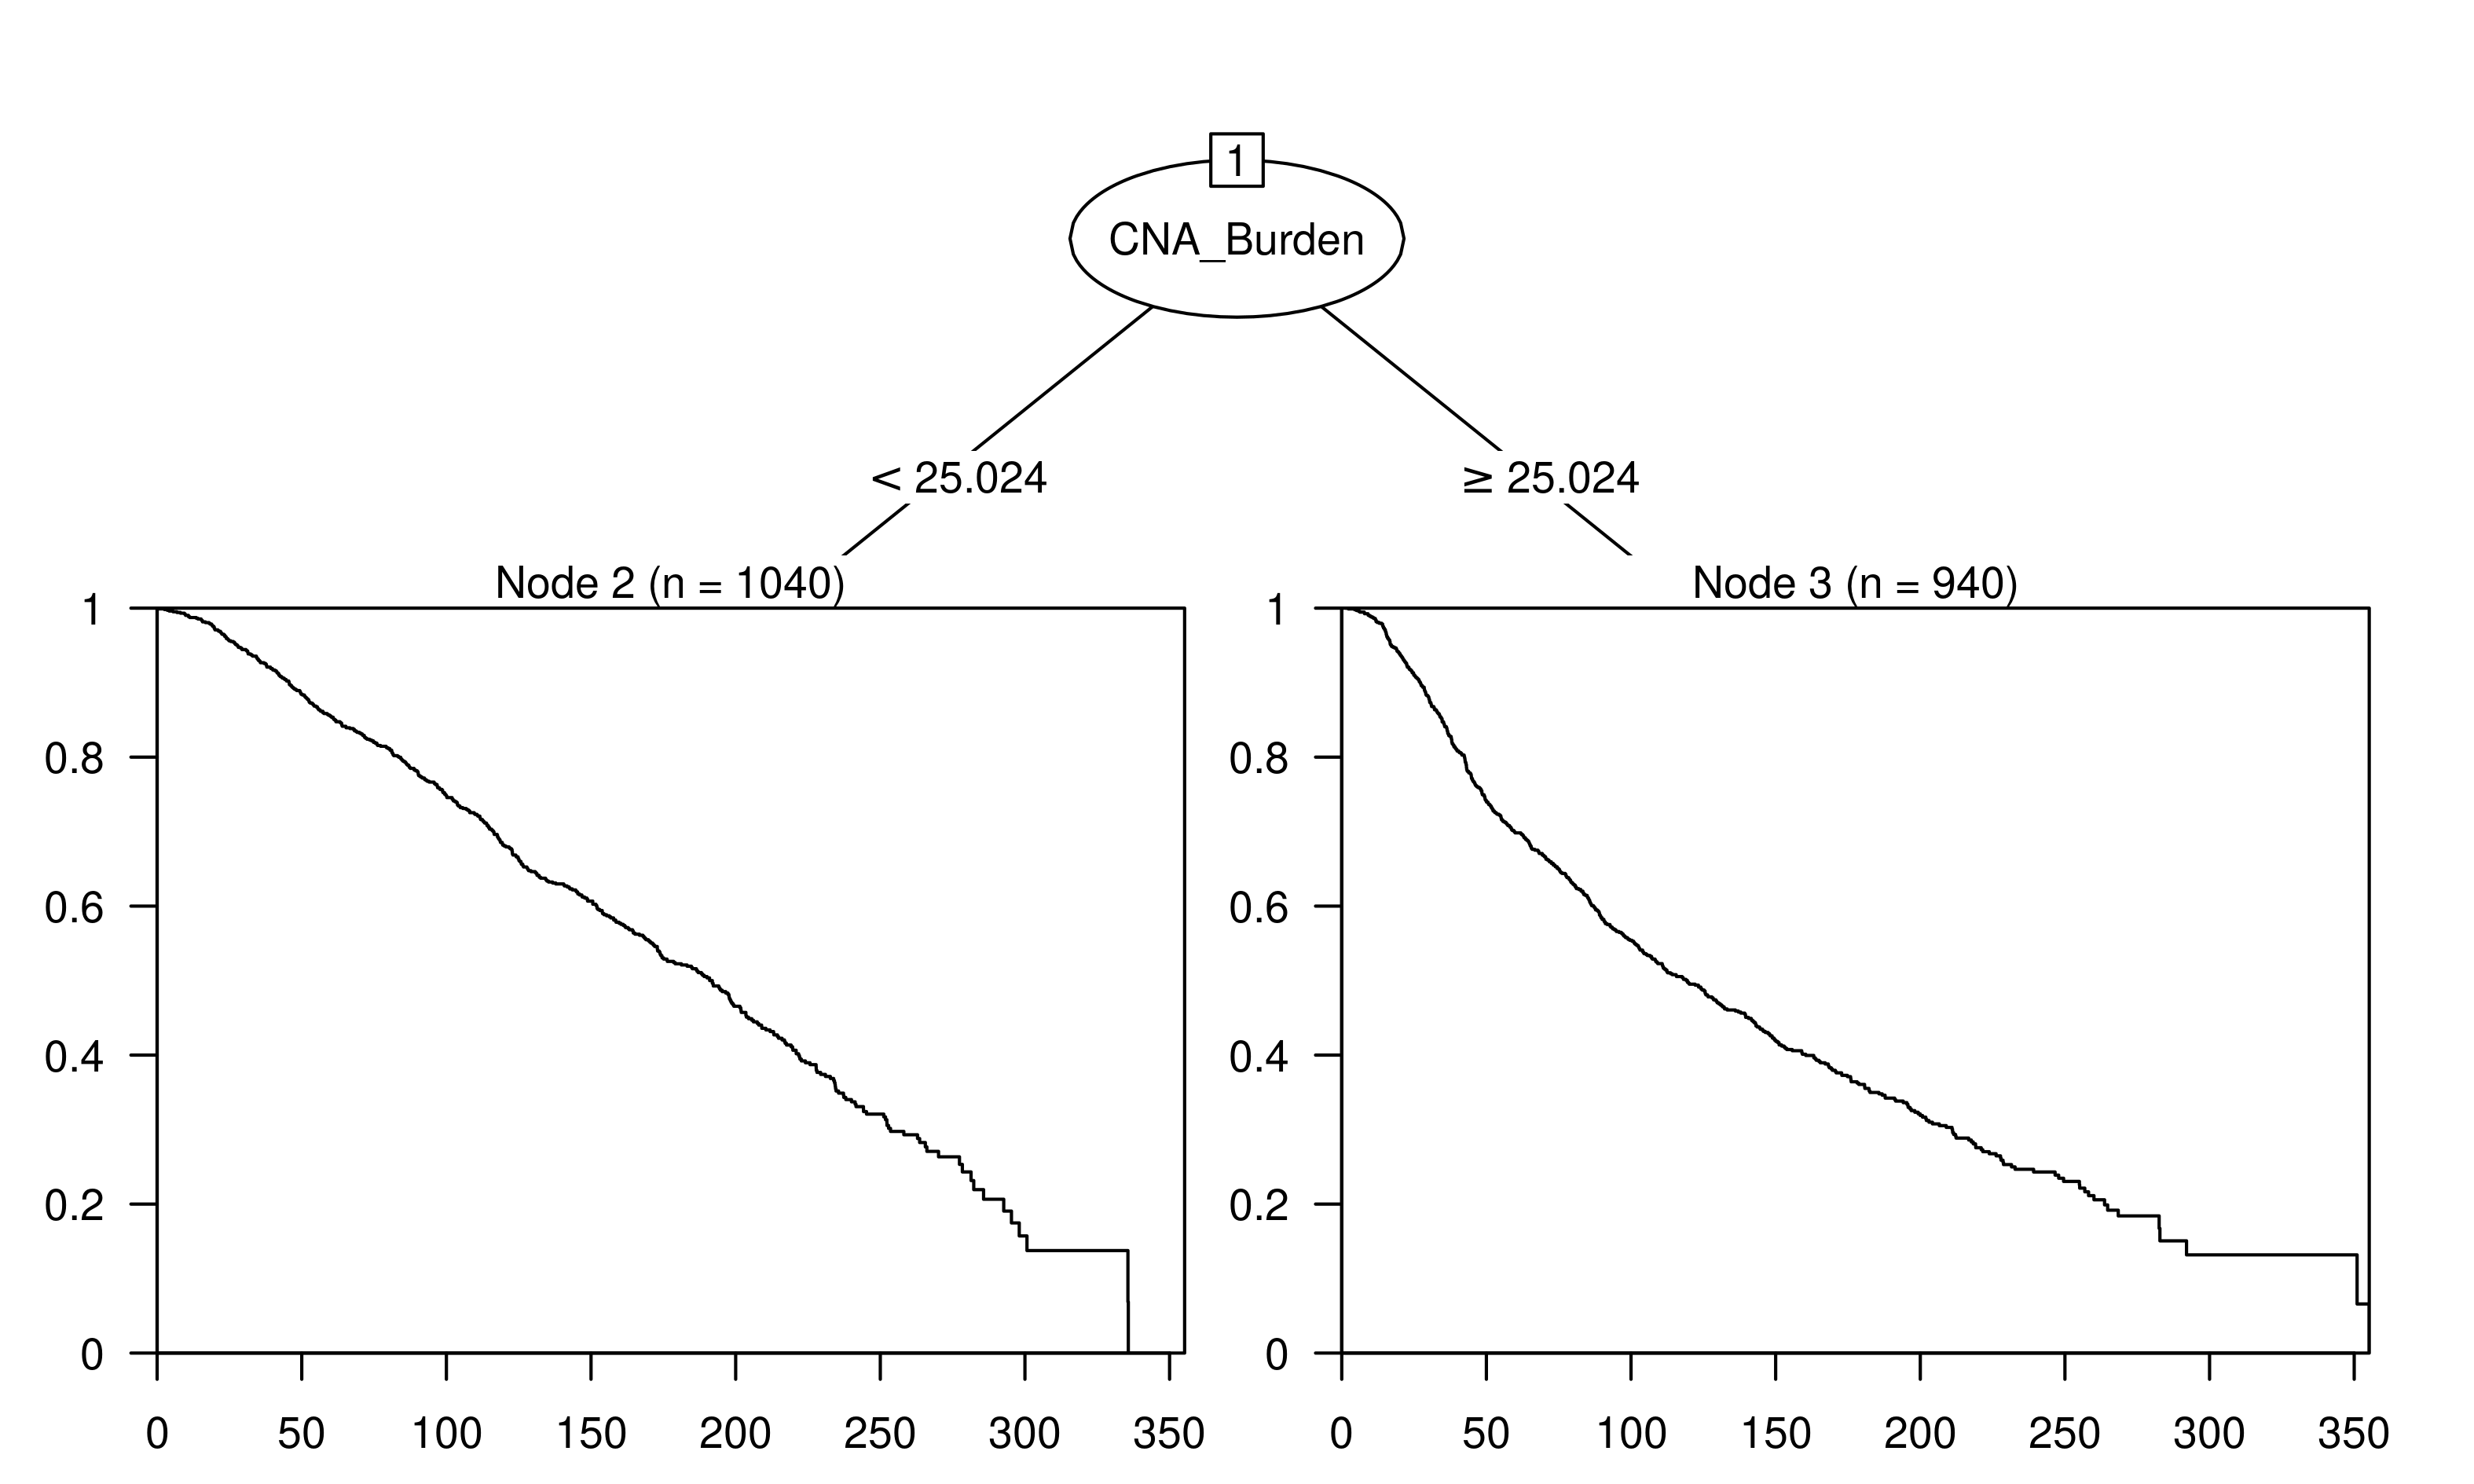
\includegraphics[width=1\textwidth]{../figures/Appendices/Appendix_B/PartyKit_Survival_Burden_OS_PAM50.png}
\end{subfigure}

\vspace{2cm}

\begin{subfigure}{\textwidth}
\subcaption{}
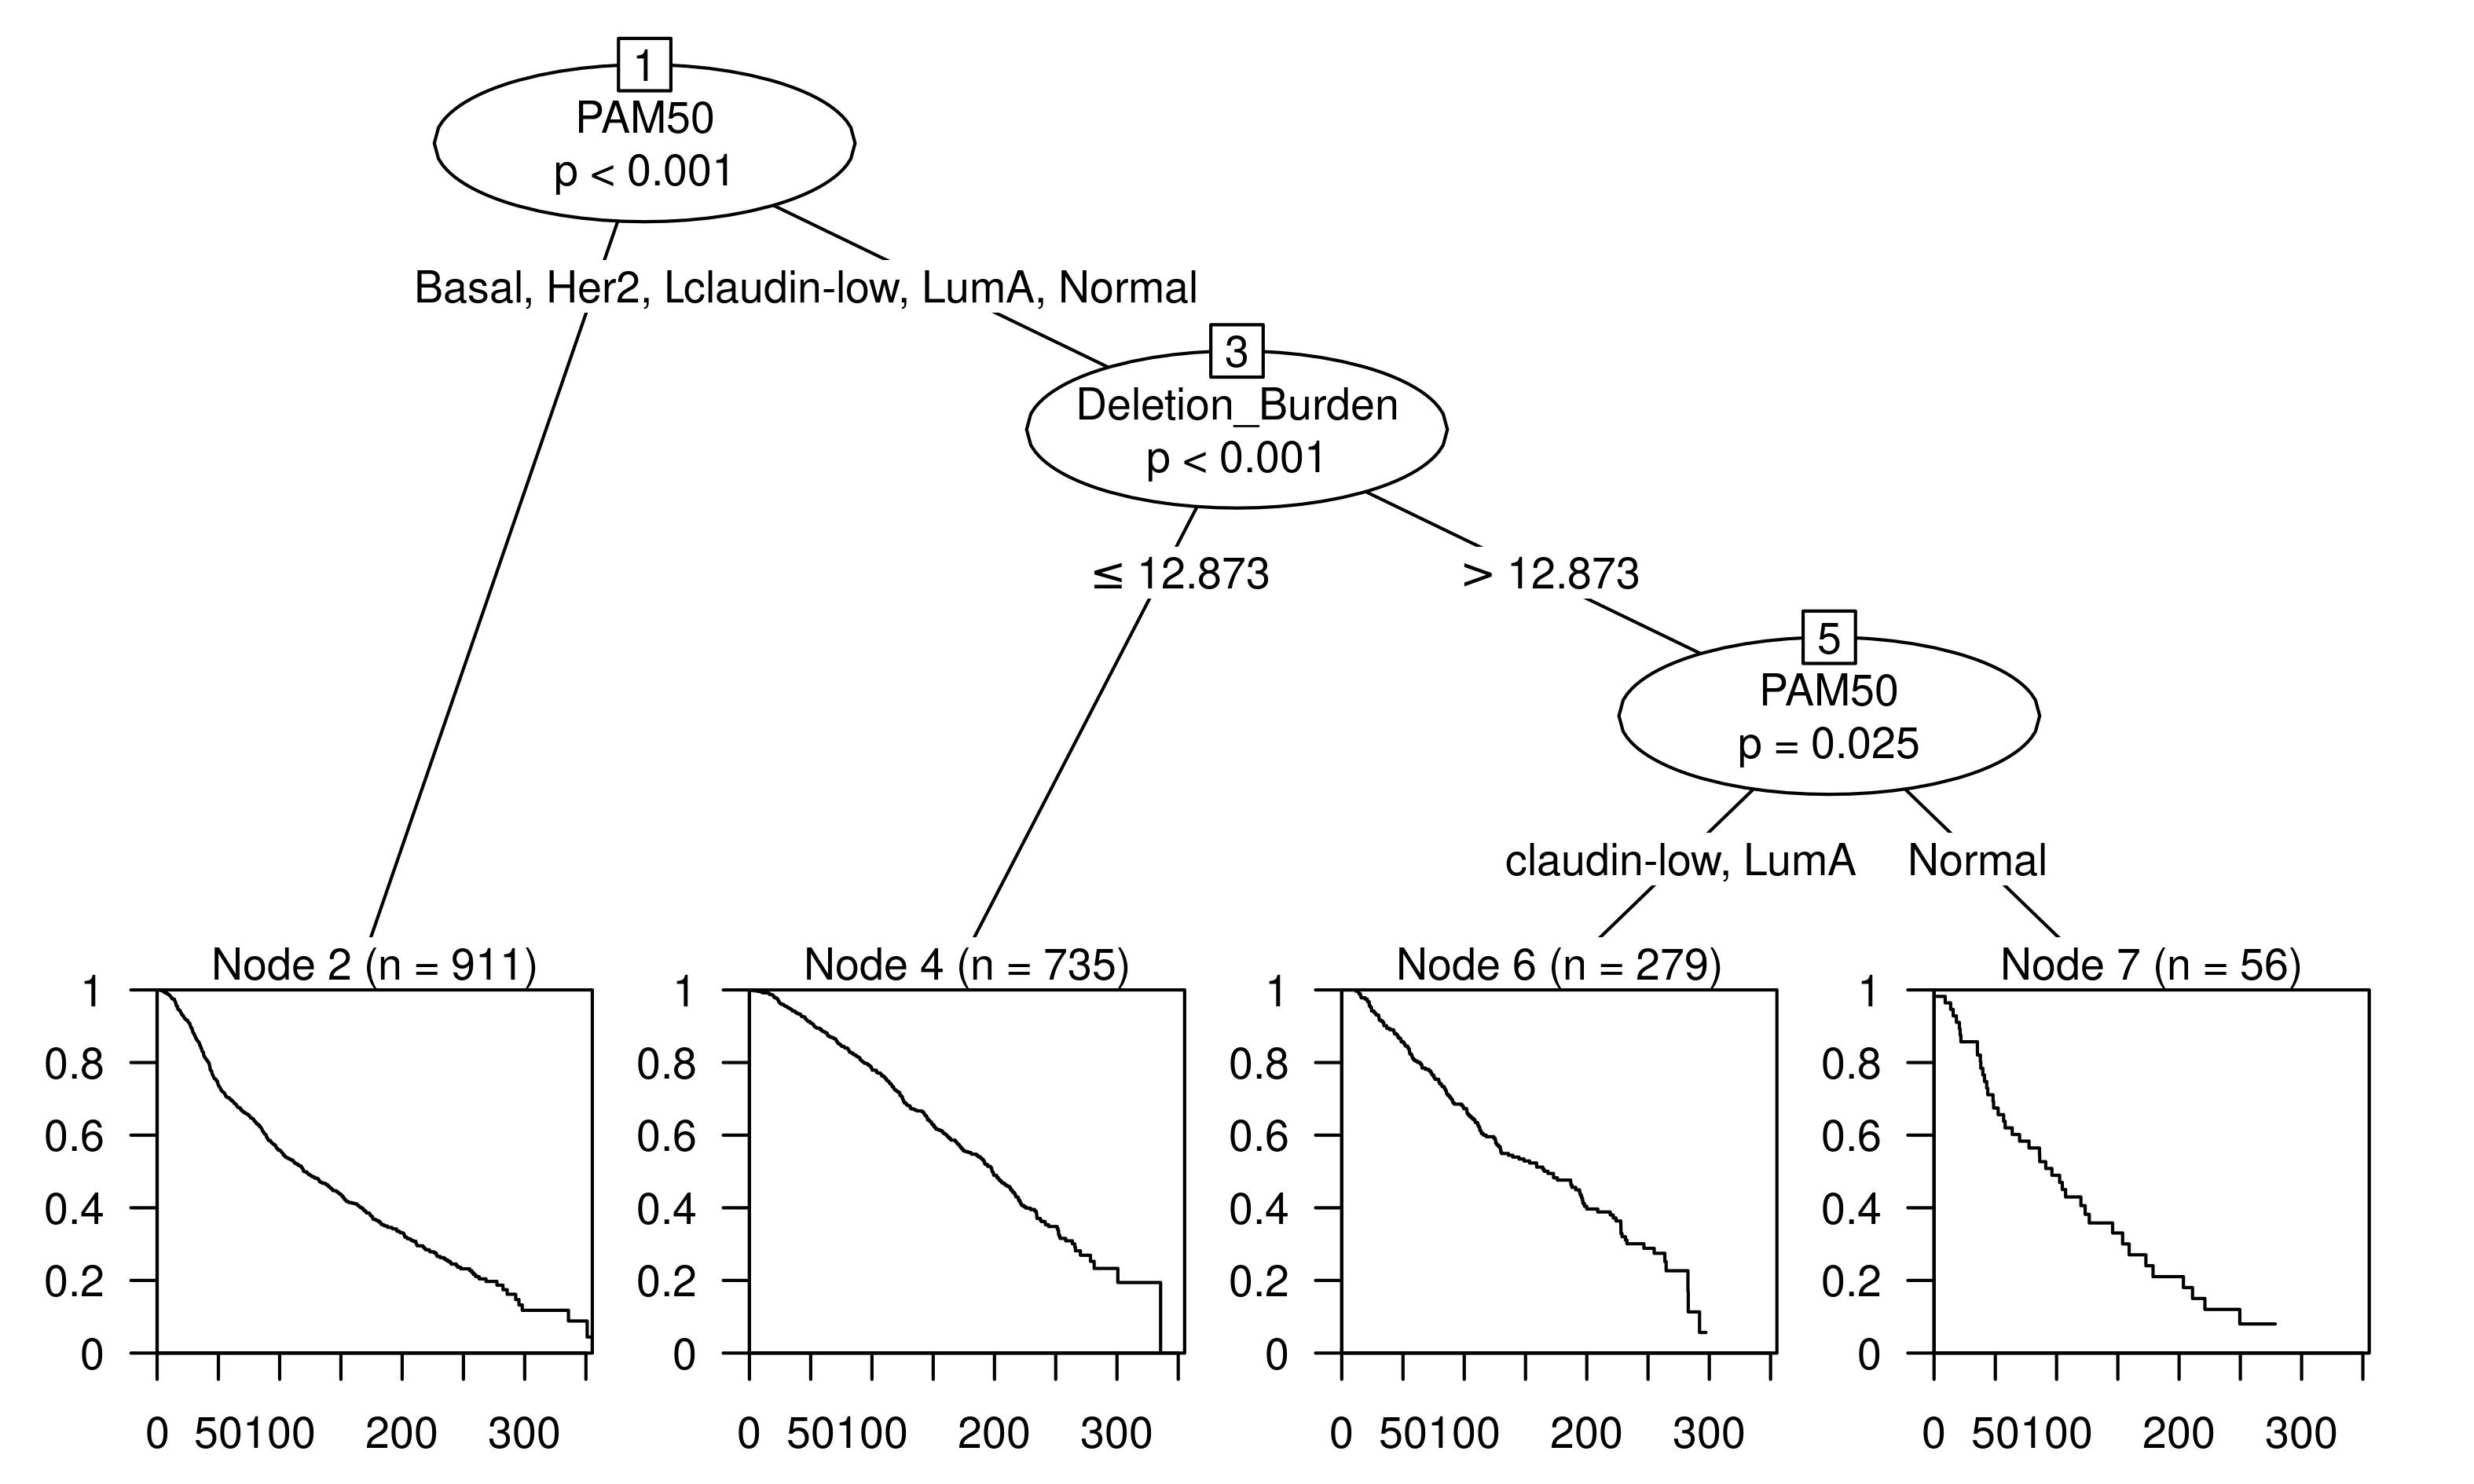
\includegraphics[width=1\textwidth]{../figures/Appendices/Appendix_B/Ctree_Survival_Burden_OS_PAM50.png}
\end{subfigure}

\vspace{0.5cm}

\caption[Recursive partitioning survival trees for overall survival using PAM50 and the six CNA Burden metrics as candidate predictors.]{Recursive partitioning survival trees for overall survival using PAM50 and the six CNA Burden metrics as candidate predictors. (A) Trees fitted using the rpart algorithm and (B) trees fitted using the ctree algorithm.}
\end{figure}

\begin{figure}[!htb]
\centering

\vspace{0.5cm}

\begin{subfigure}{\textwidth}
\subcaption{}
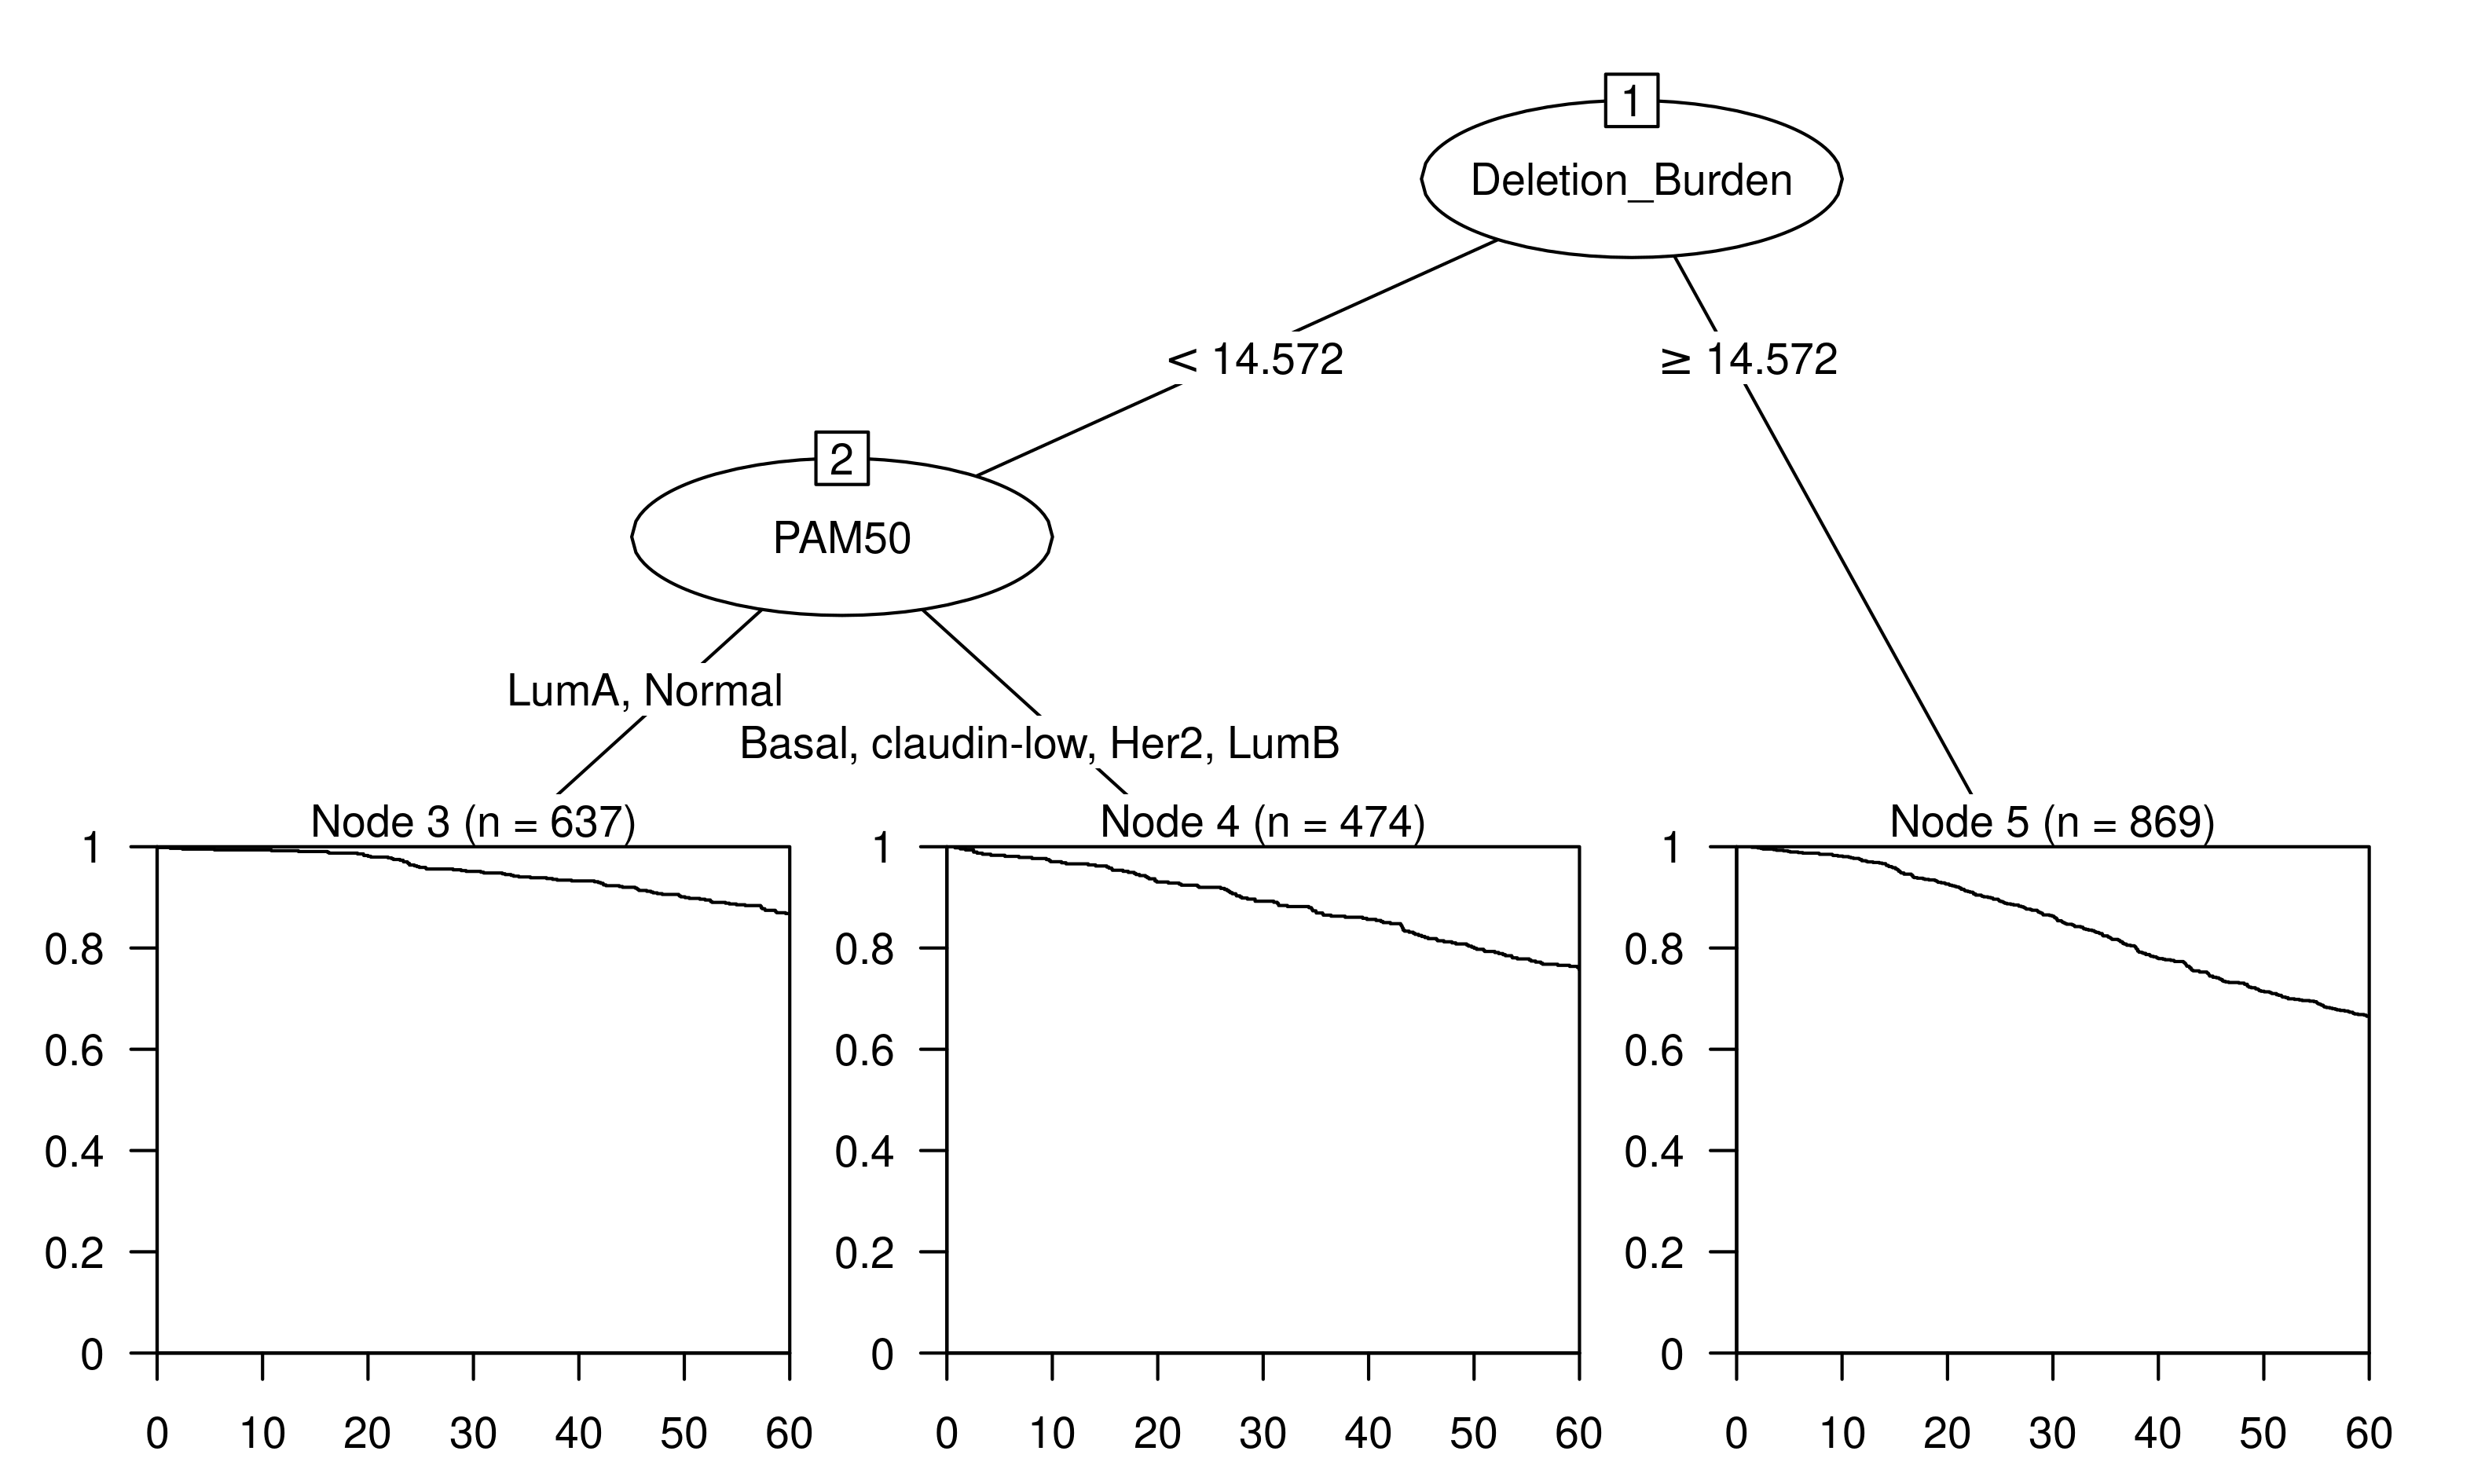
\includegraphics[width=1\textwidth]{../figures/Appendices/Appendix_B/PartyKit_Survival_Burden_FiveYearOS_PAM50.png}
\end{subfigure}

\vspace{2cm}

\begin{subfigure}{\textwidth}
\subcaption{}
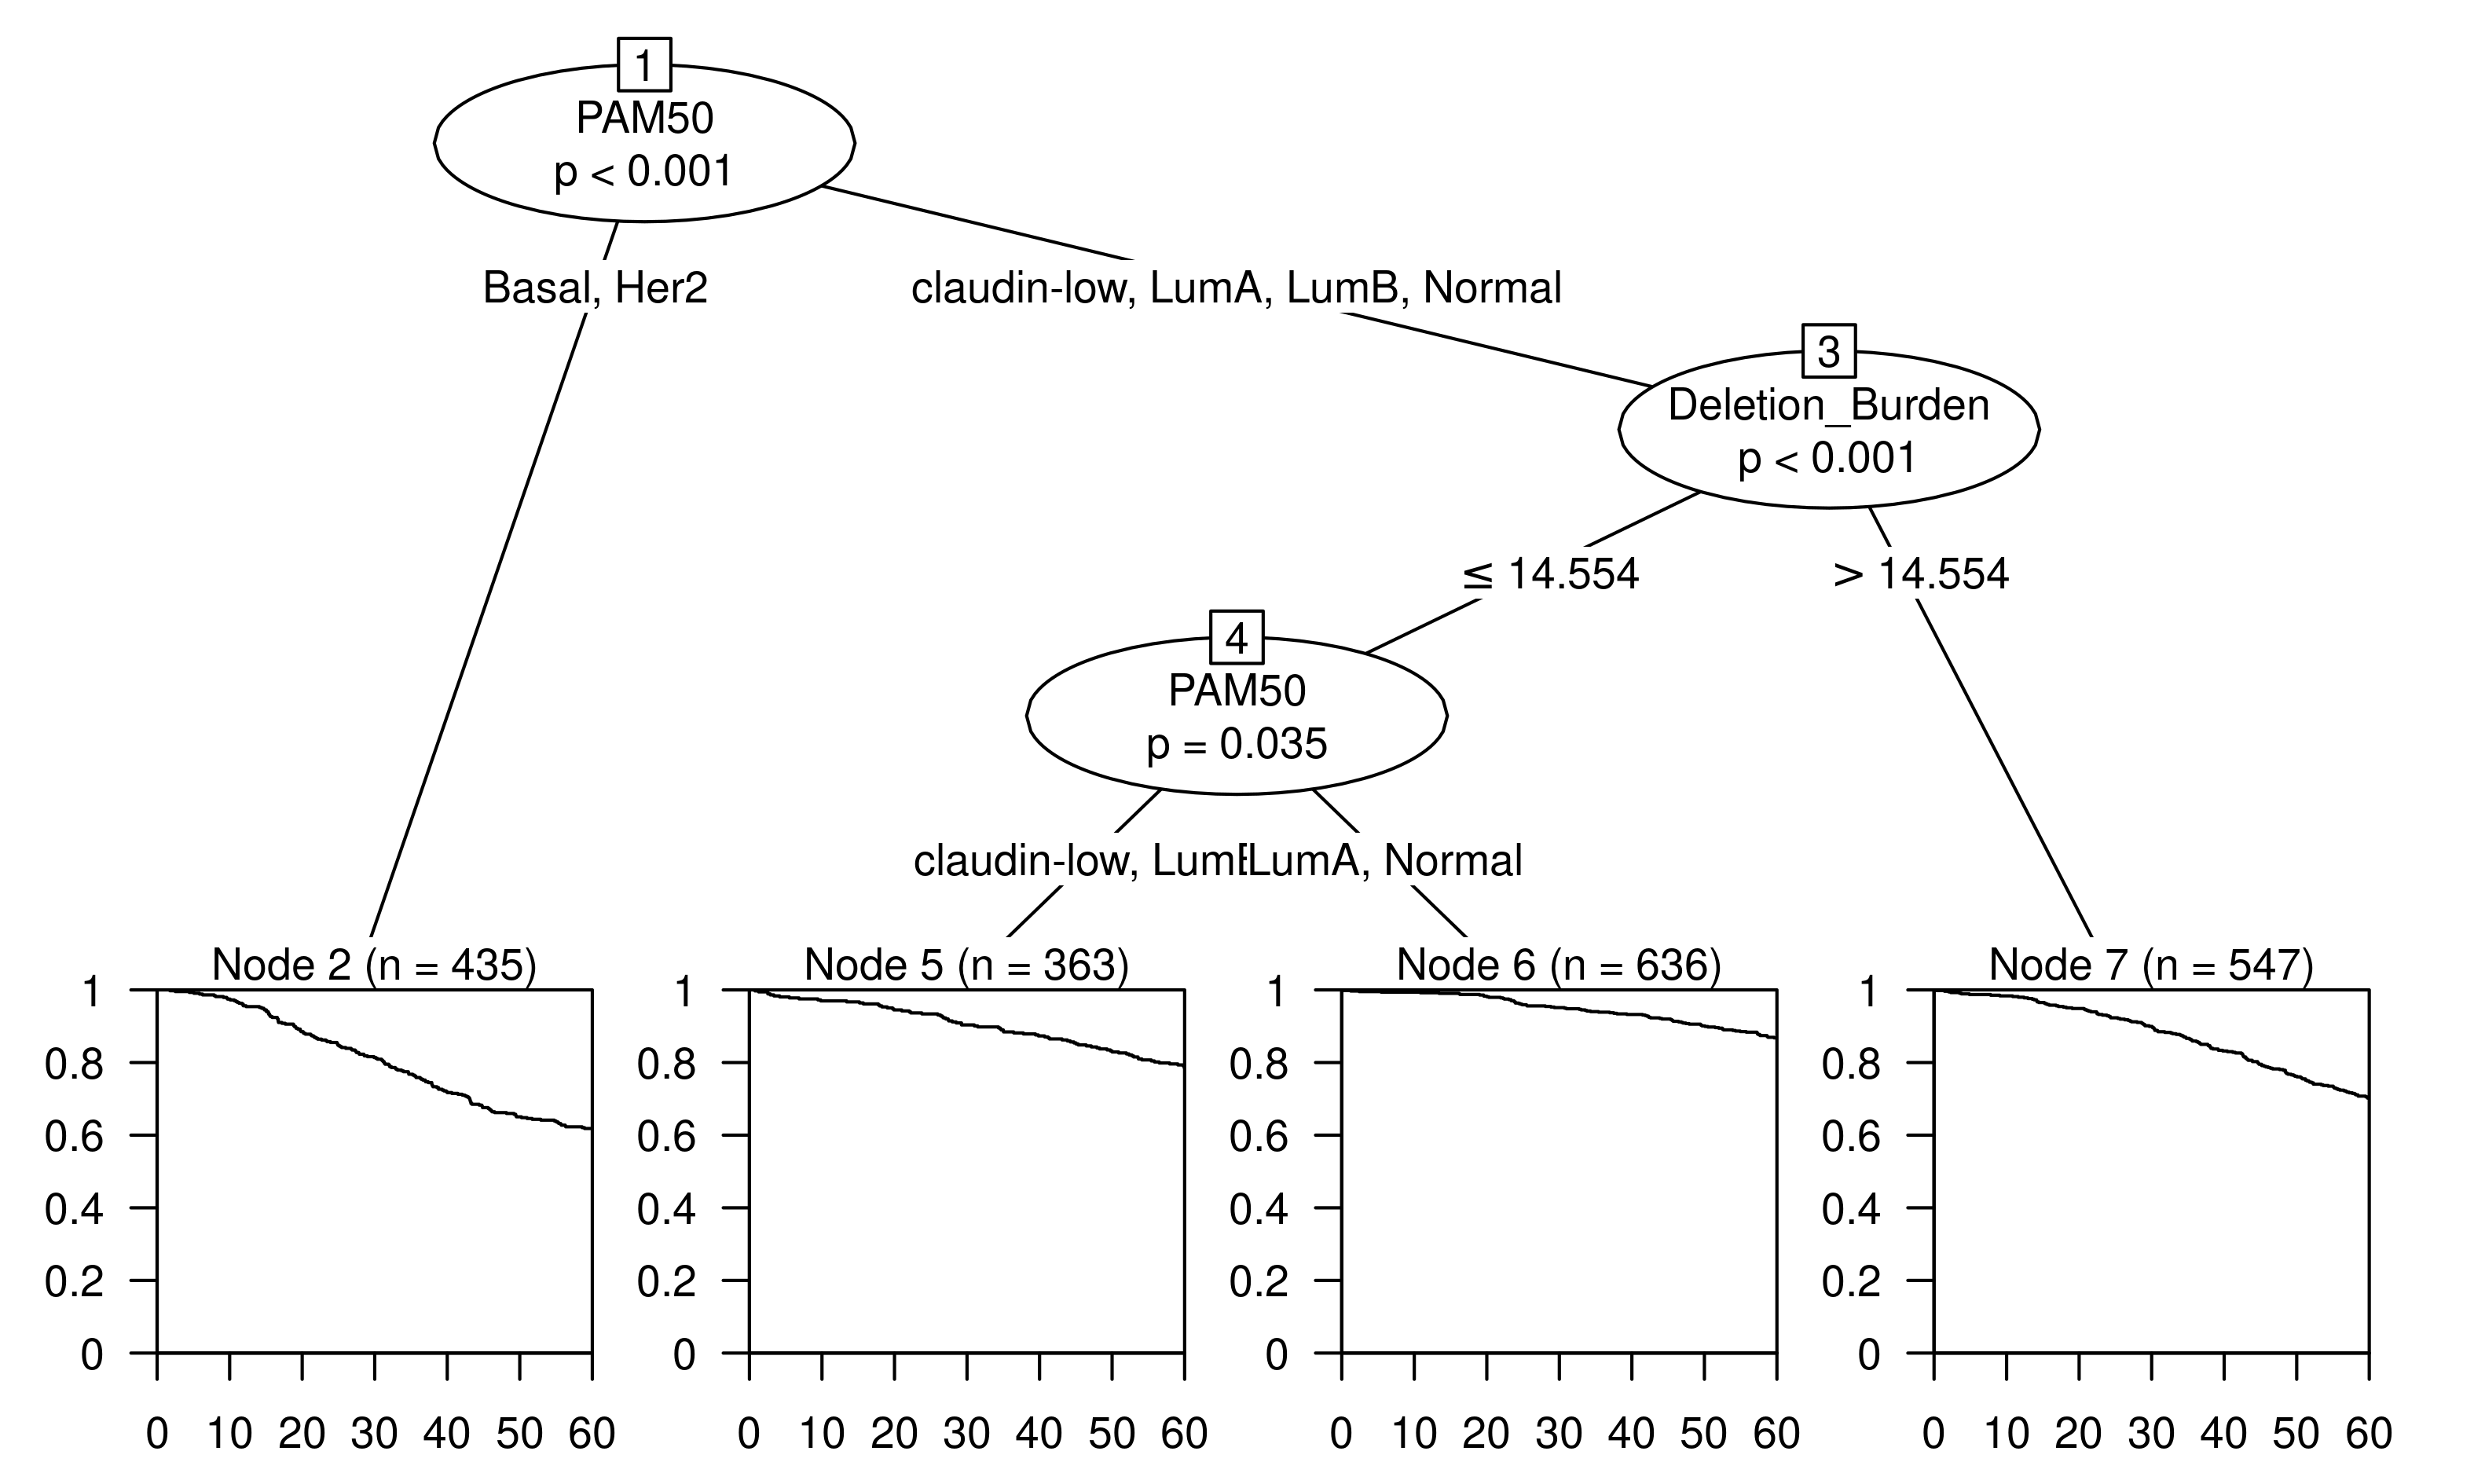
\includegraphics[width=1\textwidth]{../figures/Appendices/Appendix_B/Ctree_Survival_Burden_FiveYearOS_PAM50.png}
\end{subfigure}

\vspace{0.5cm}

\caption[Recursive partitioning survival trees for five-year overall survival using PAM50 and the six CNA Burden metrics as candidate predictors.]{Recursive partitioning survival trees for five-year overall survival using PAM50 and the six CNA Burden metrics as candidate predictors. (A) Trees fitted using the rpart algorithm and (B) trees fitted using the ctree algorithm.}
\end{figure}

\begin{figure}[!htb]
\centering

\vspace{0.5cm}

\begin{subfigure}{\textwidth}
\subcaption{}
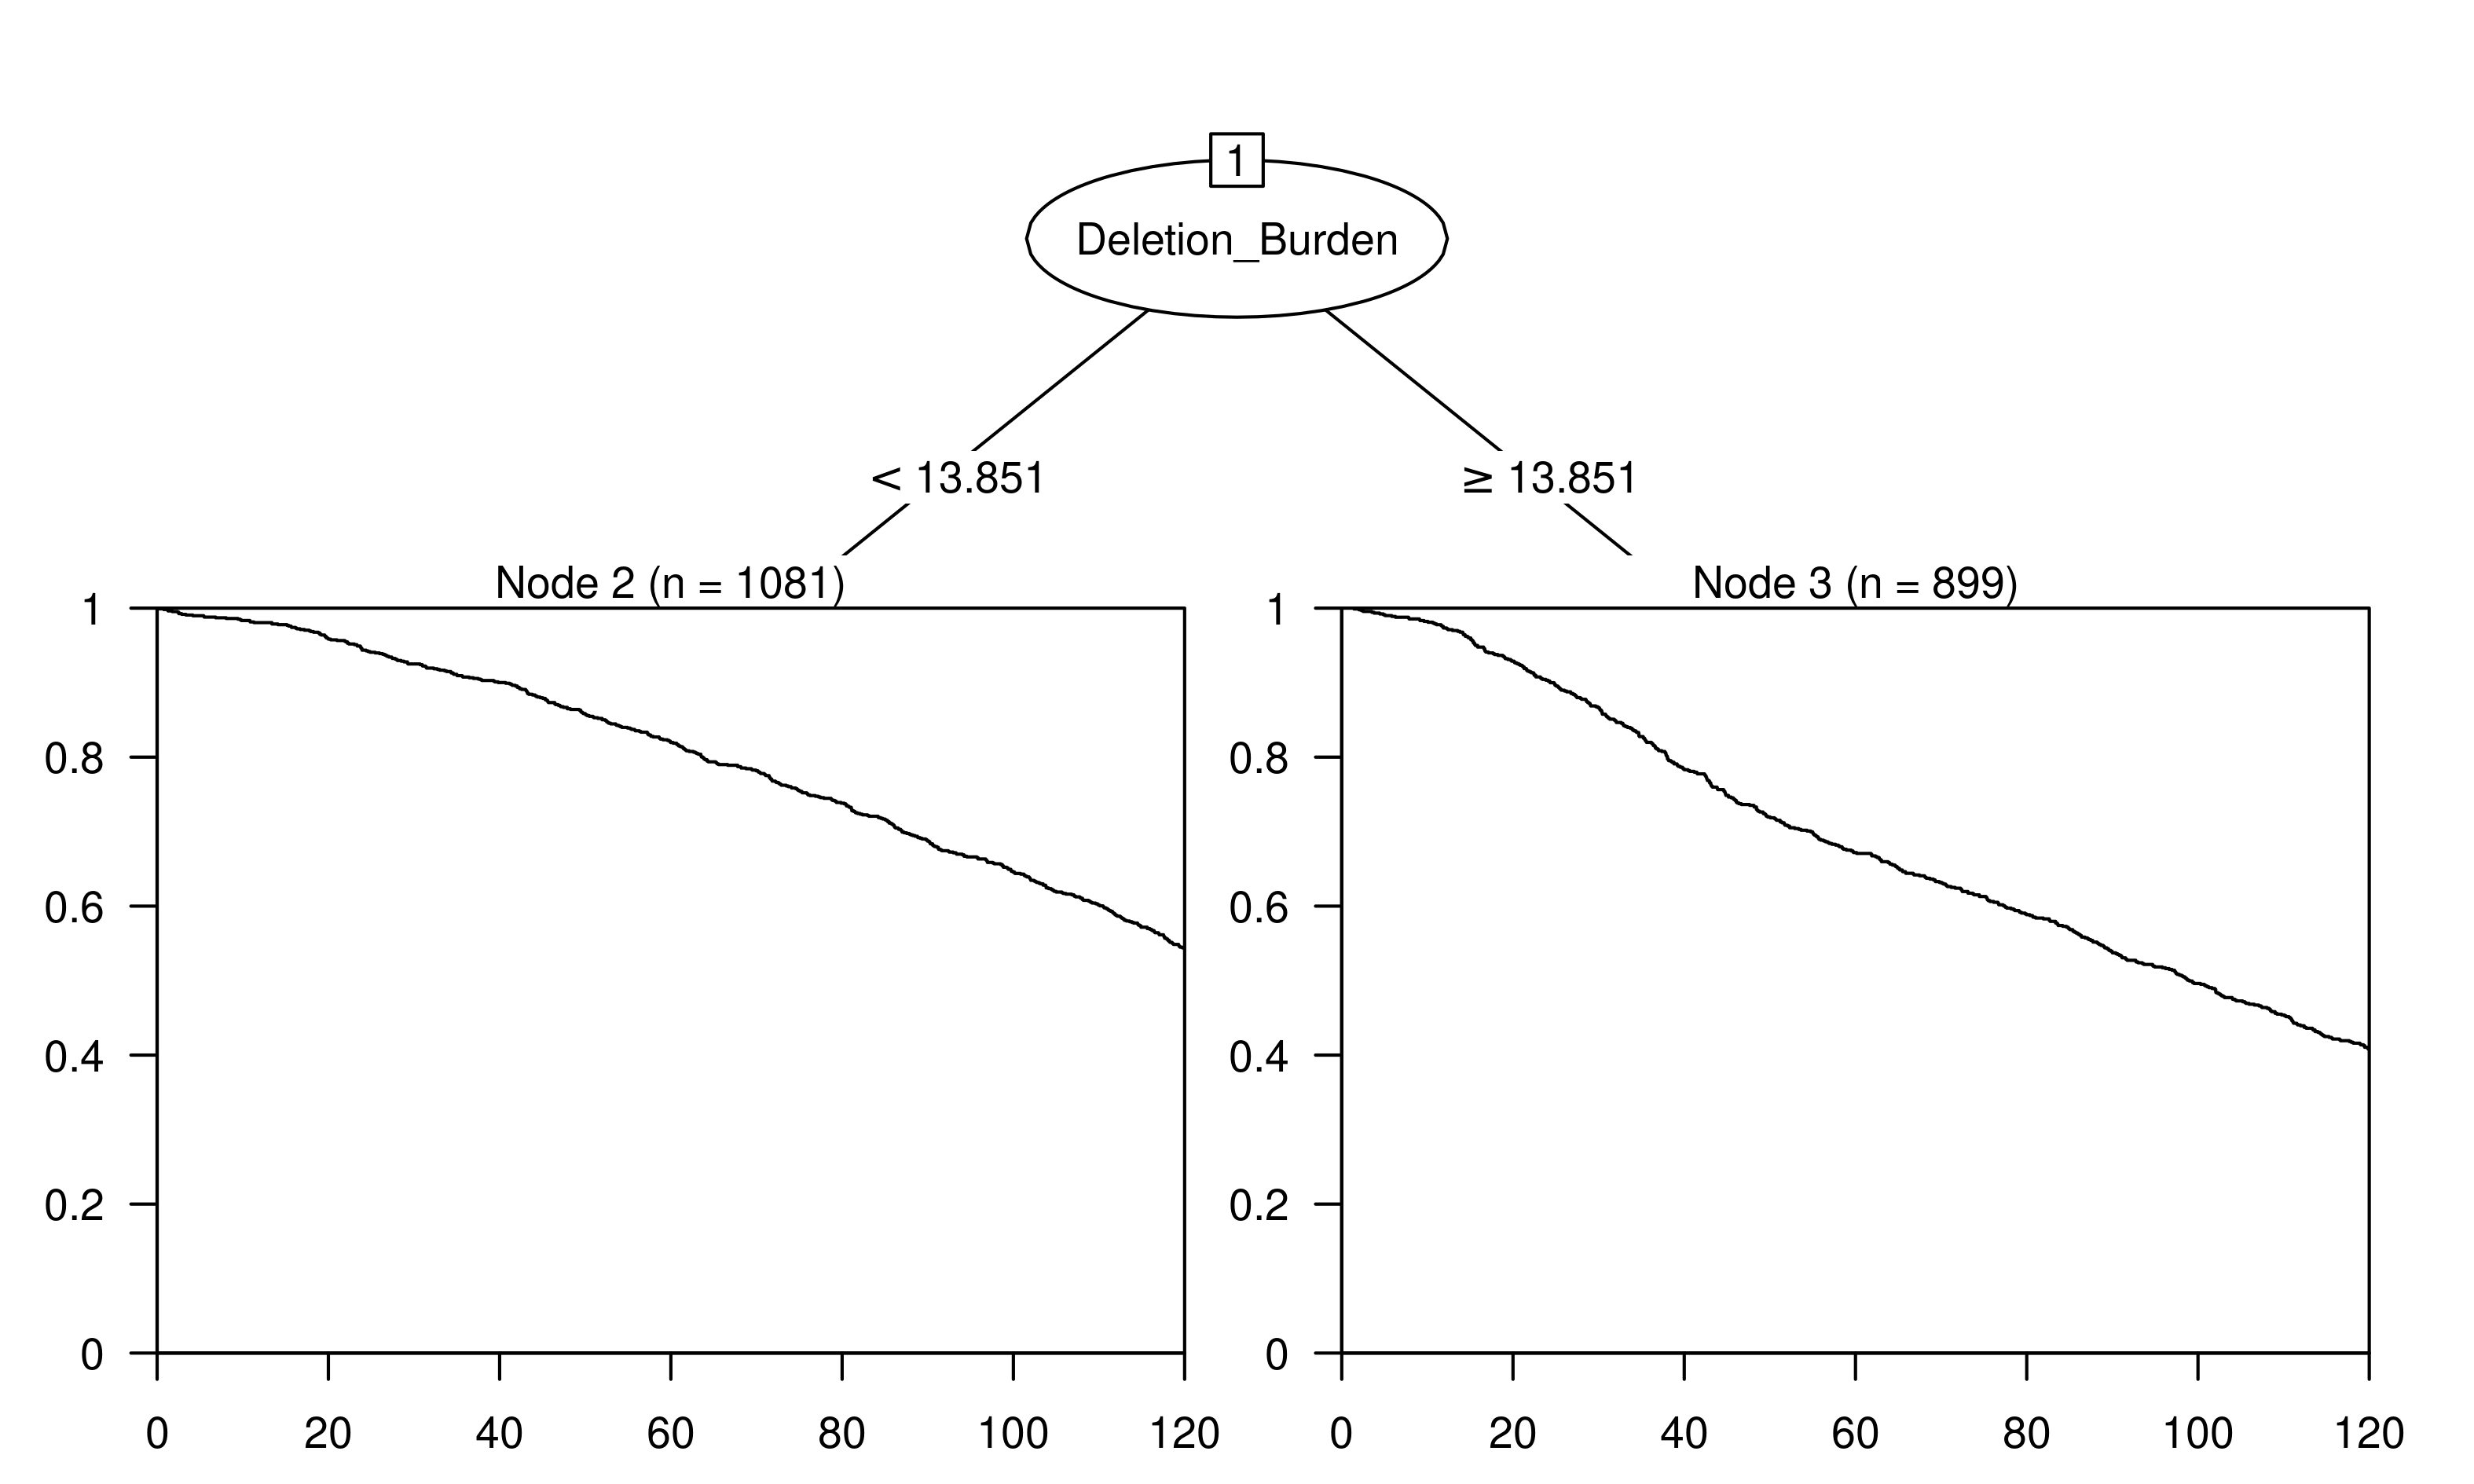
\includegraphics[width=1\textwidth]{../figures/Appendices/Appendix_B/PartyKit_Survival_Burden_TenYearOS_PAM50.png}
\end{subfigure}

\vspace{2cm}

\begin{subfigure}{\textwidth}
\subcaption{}
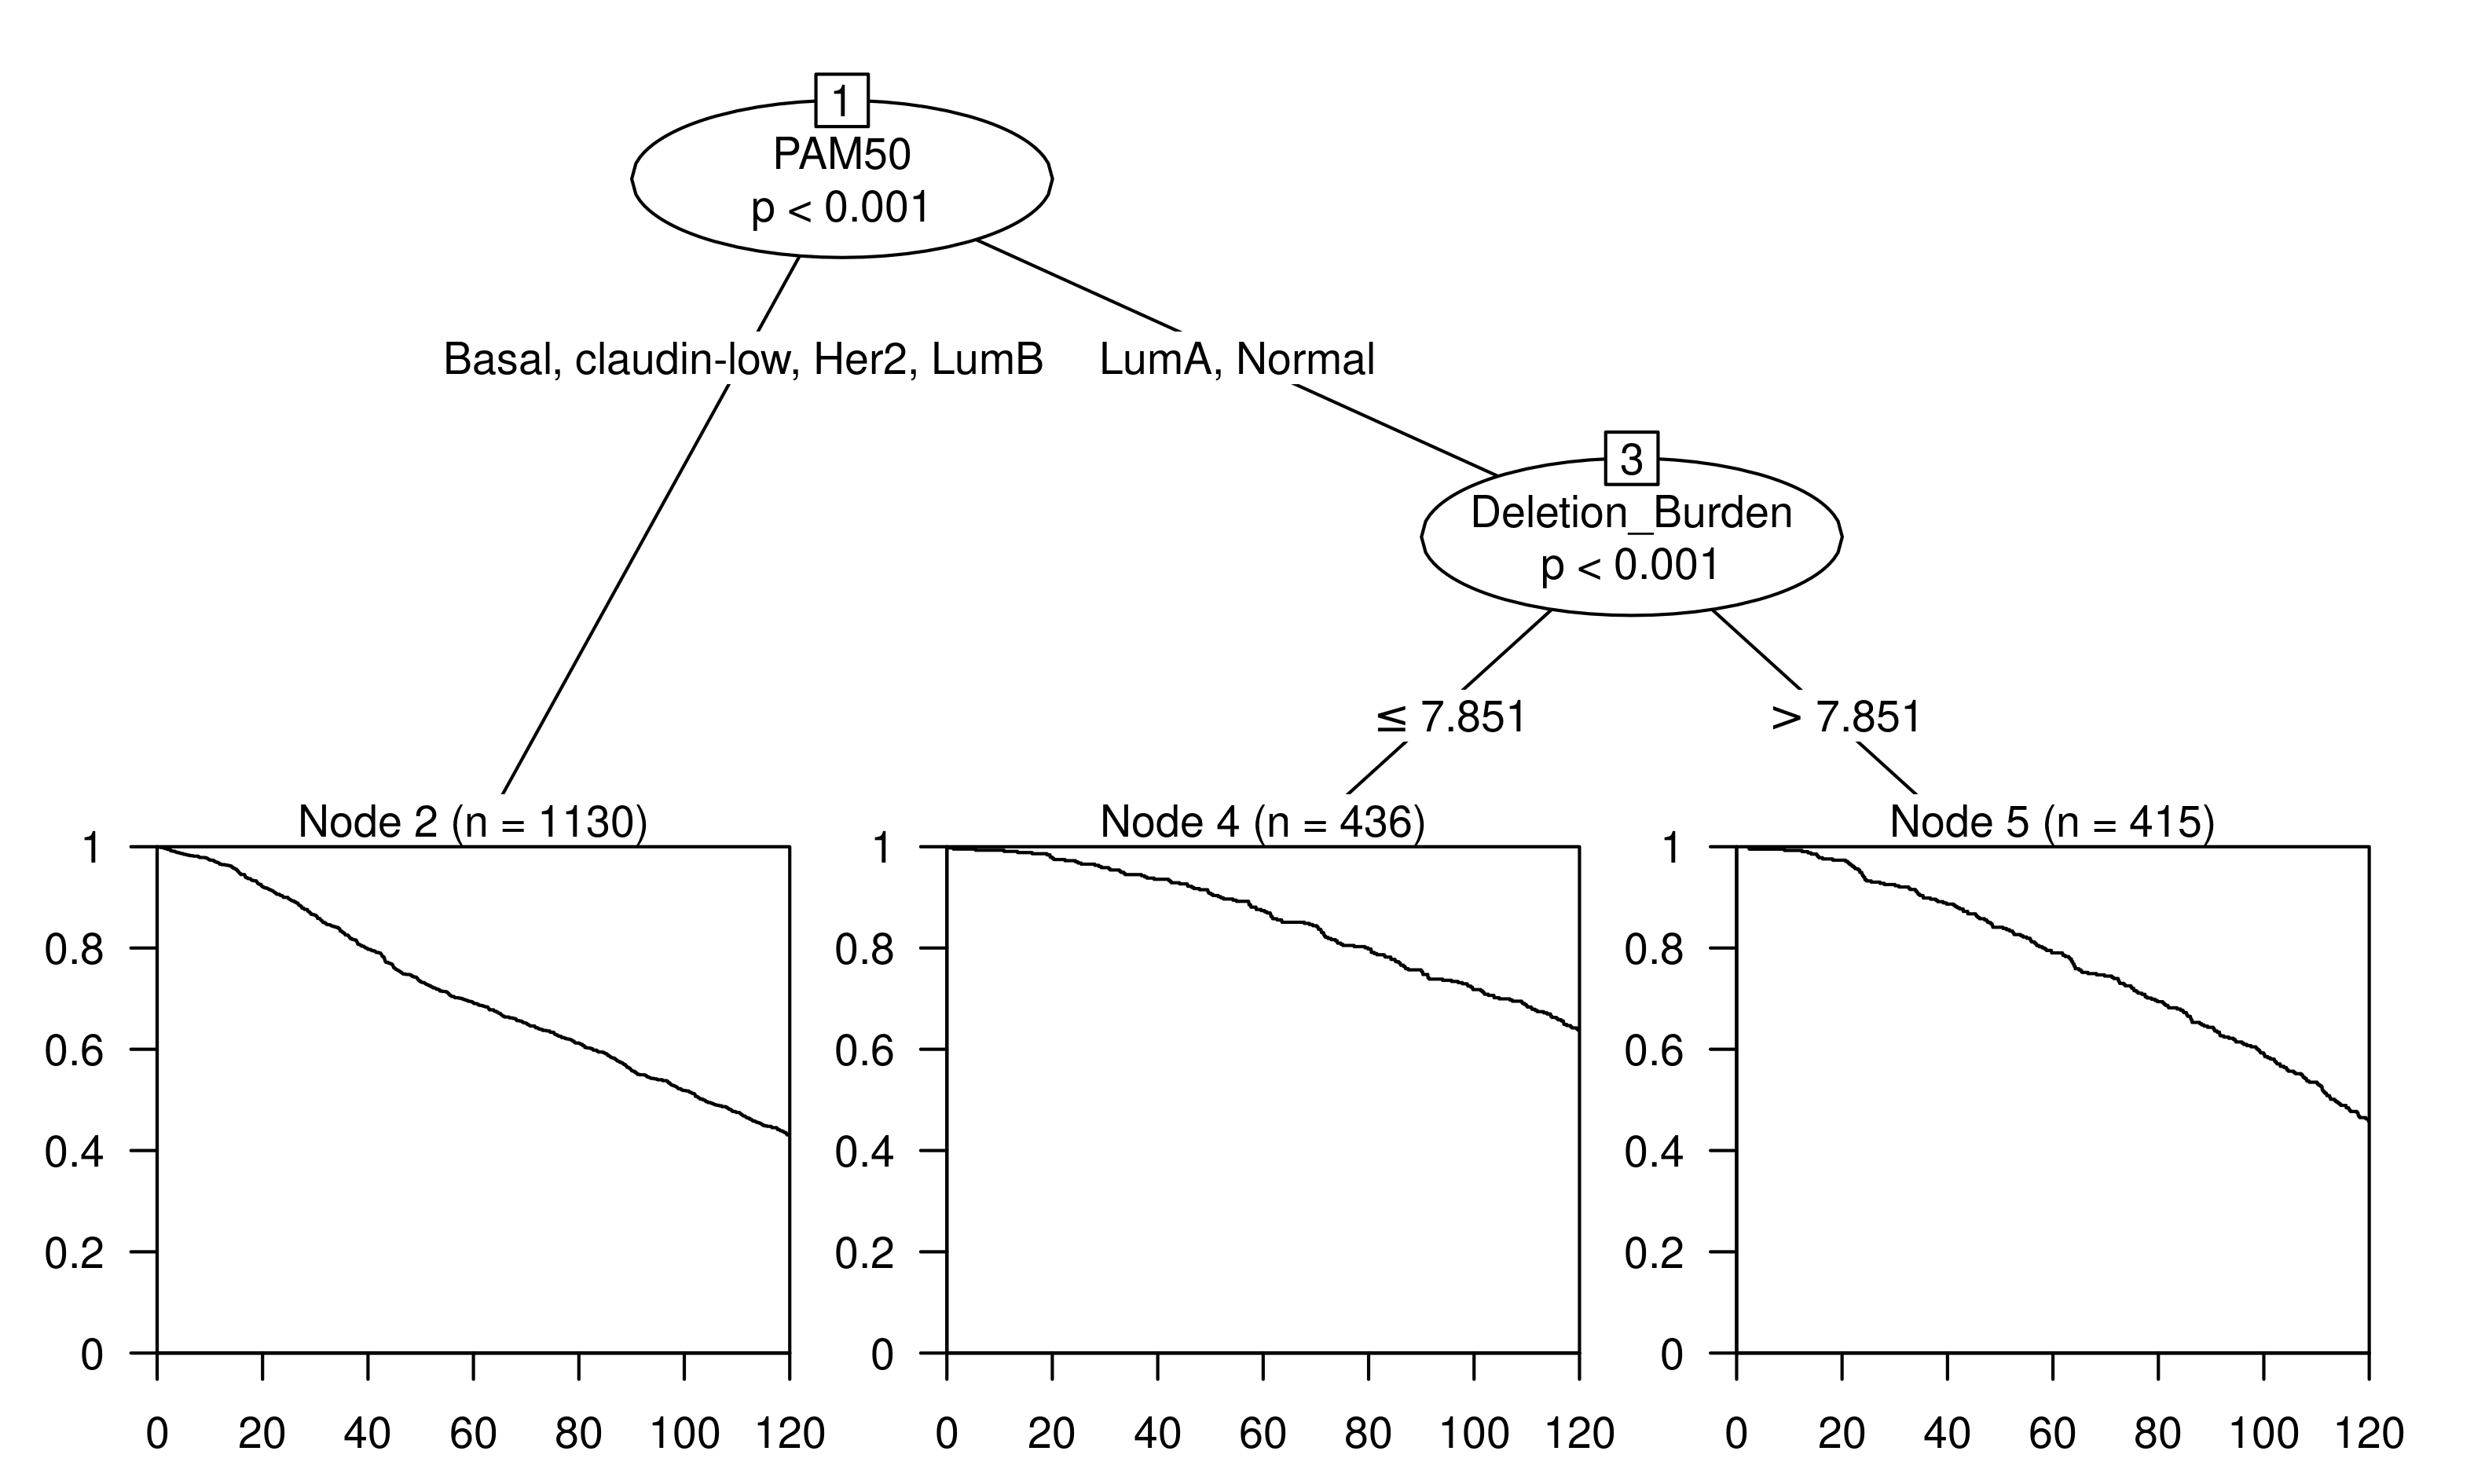
\includegraphics[width=1\textwidth]{../figures/Appendices/Appendix_B/Ctree_Survival_Burden_TenYearOS_PAM50.png}
\end{subfigure}

\vspace{0.5cm}

\caption[Recursive partitioning survival trees for ten-year overall survival using PAM50 and the six CNA Burden metrics as candidate predictors.]{Recursive partitioning survival trees for ten-year overall survival using PAM50 and the six CNA Burden metrics as candidate predictors. (A) Trees fitted using the rpart algorithm and (B) trees fitted using the ctree algorithm.}
\end{figure}

% OS using IntClust and the six CNA Score metrics as candidate predictors
\begin{figure}[!htb]
\centering

\vspace{0.5cm}

\begin{subfigure}{\textwidth}
\subcaption{}
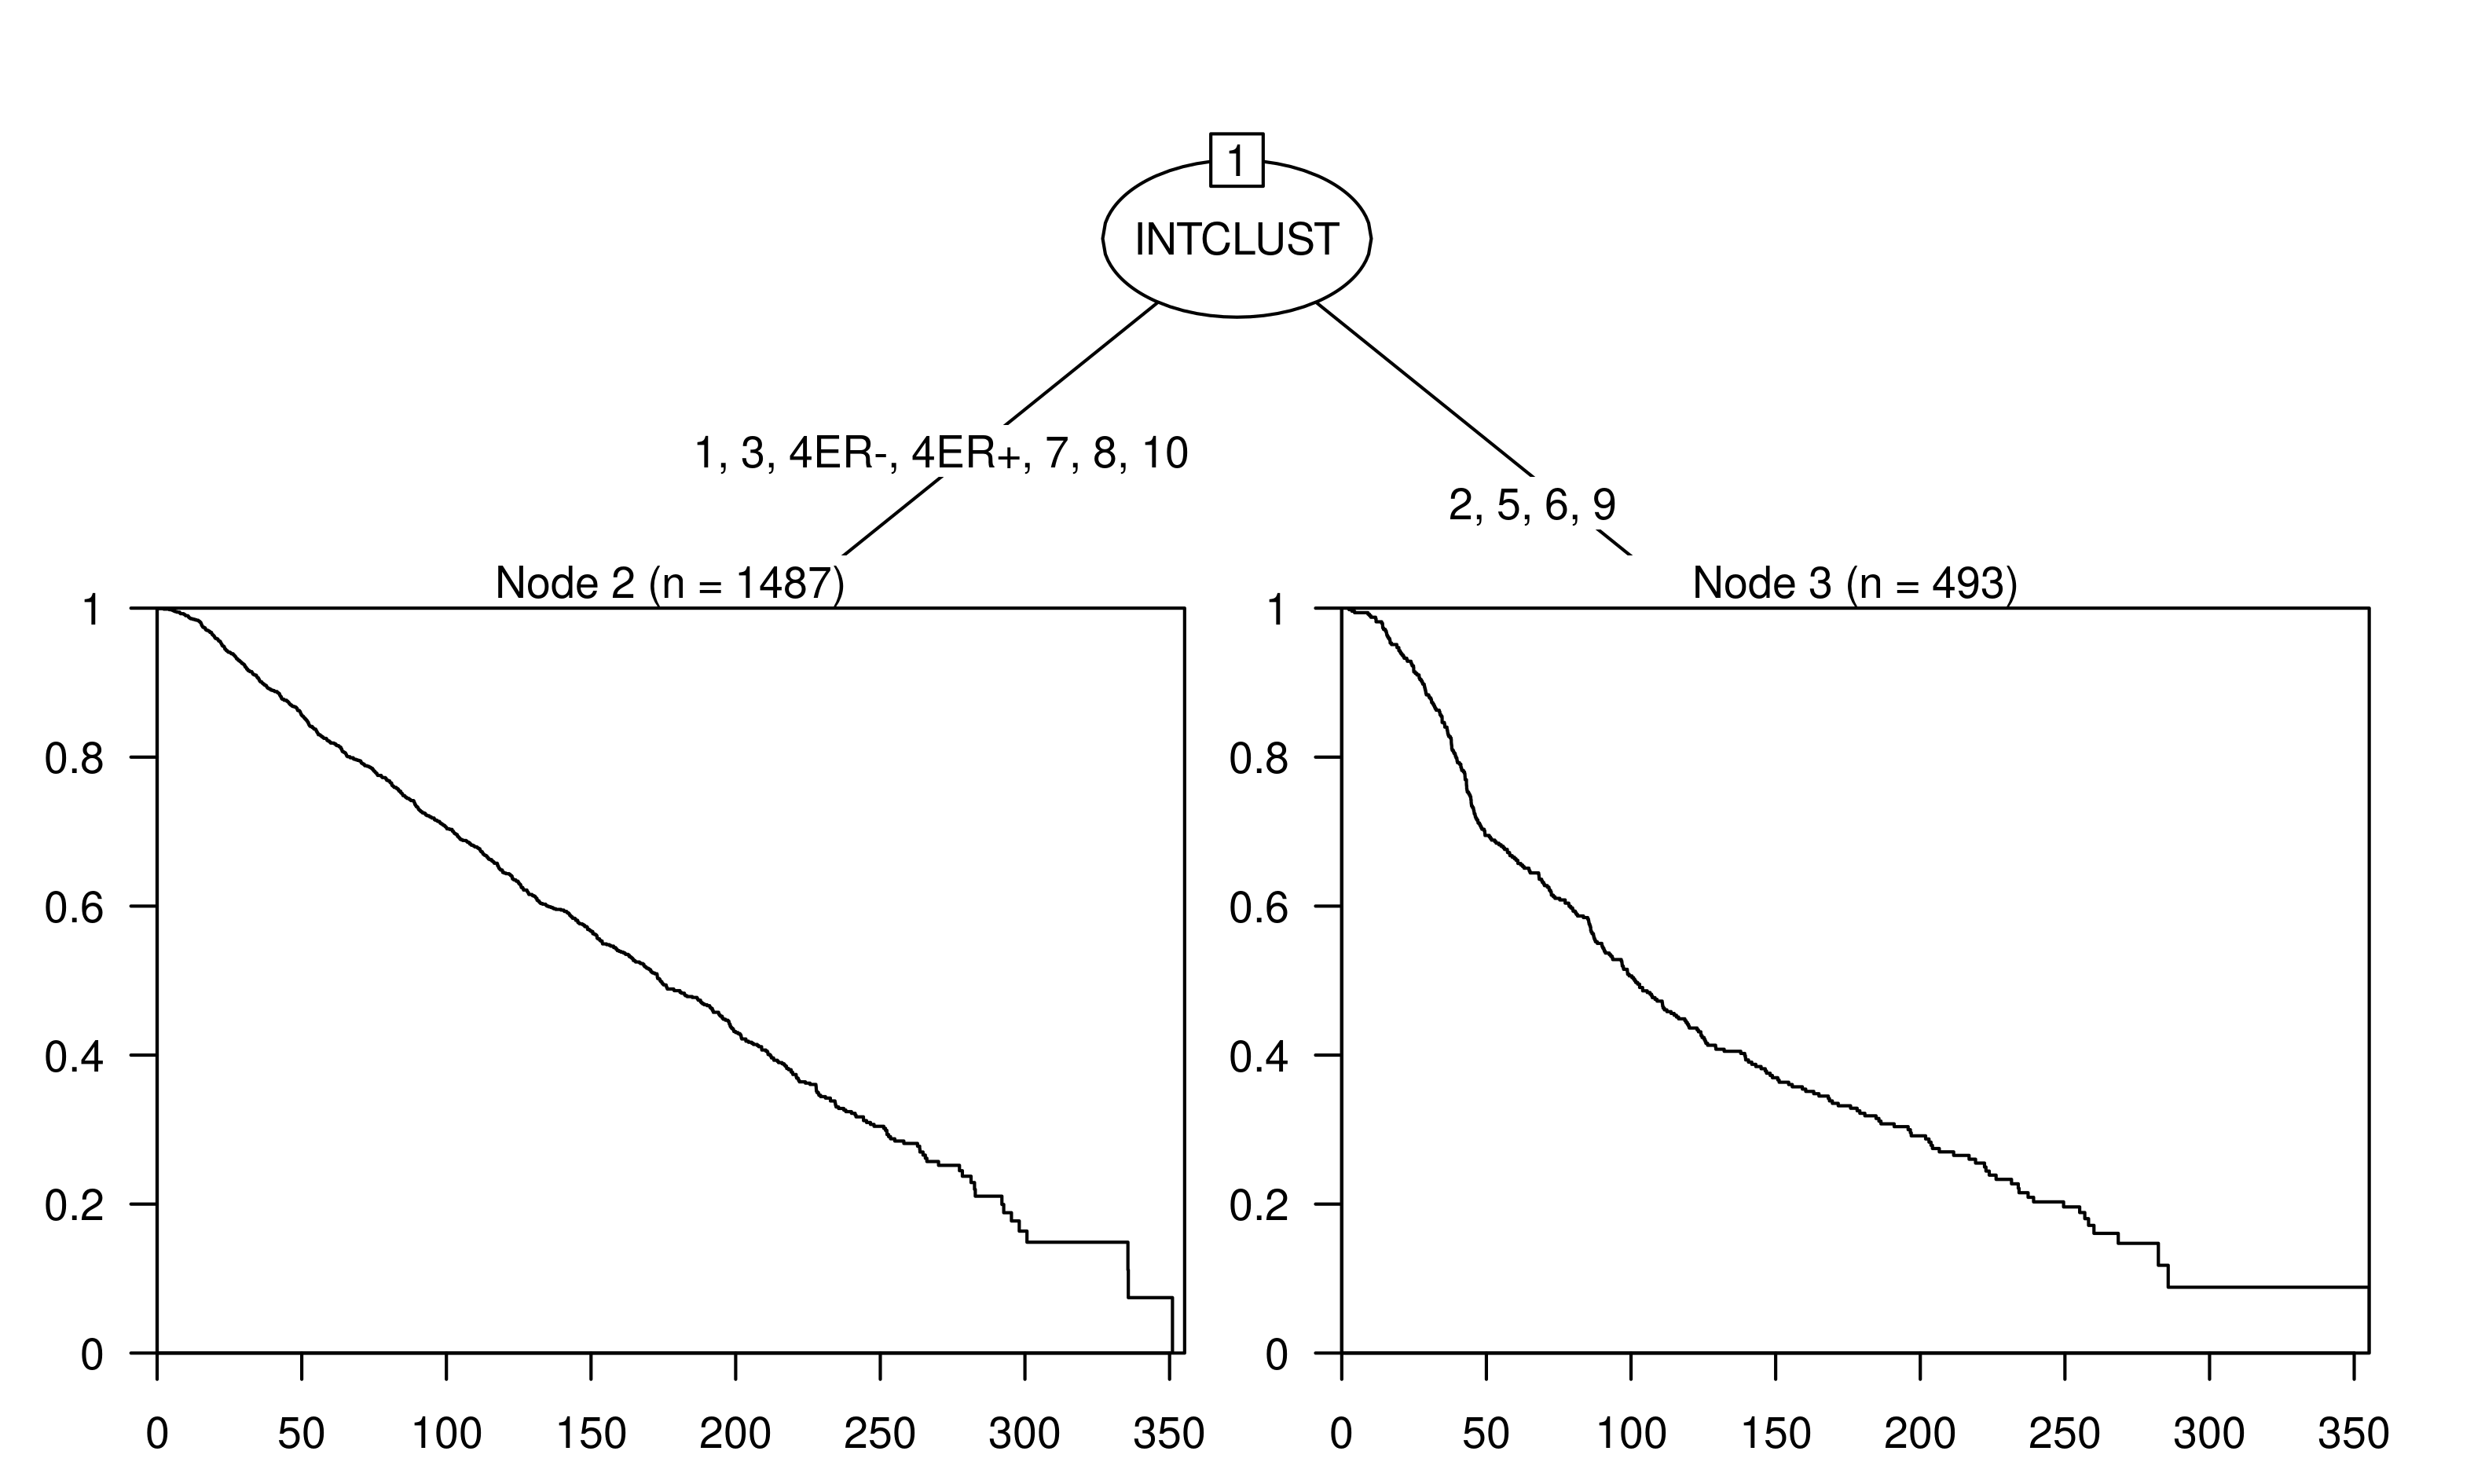
\includegraphics[width=1\textwidth]{../figures/Appendices/Appendix_B/PartyKit_Survival_Score_OS_INTCLUST.png}
\end{subfigure}

\vspace{2cm}

\begin{subfigure}{\textwidth}
\subcaption{}
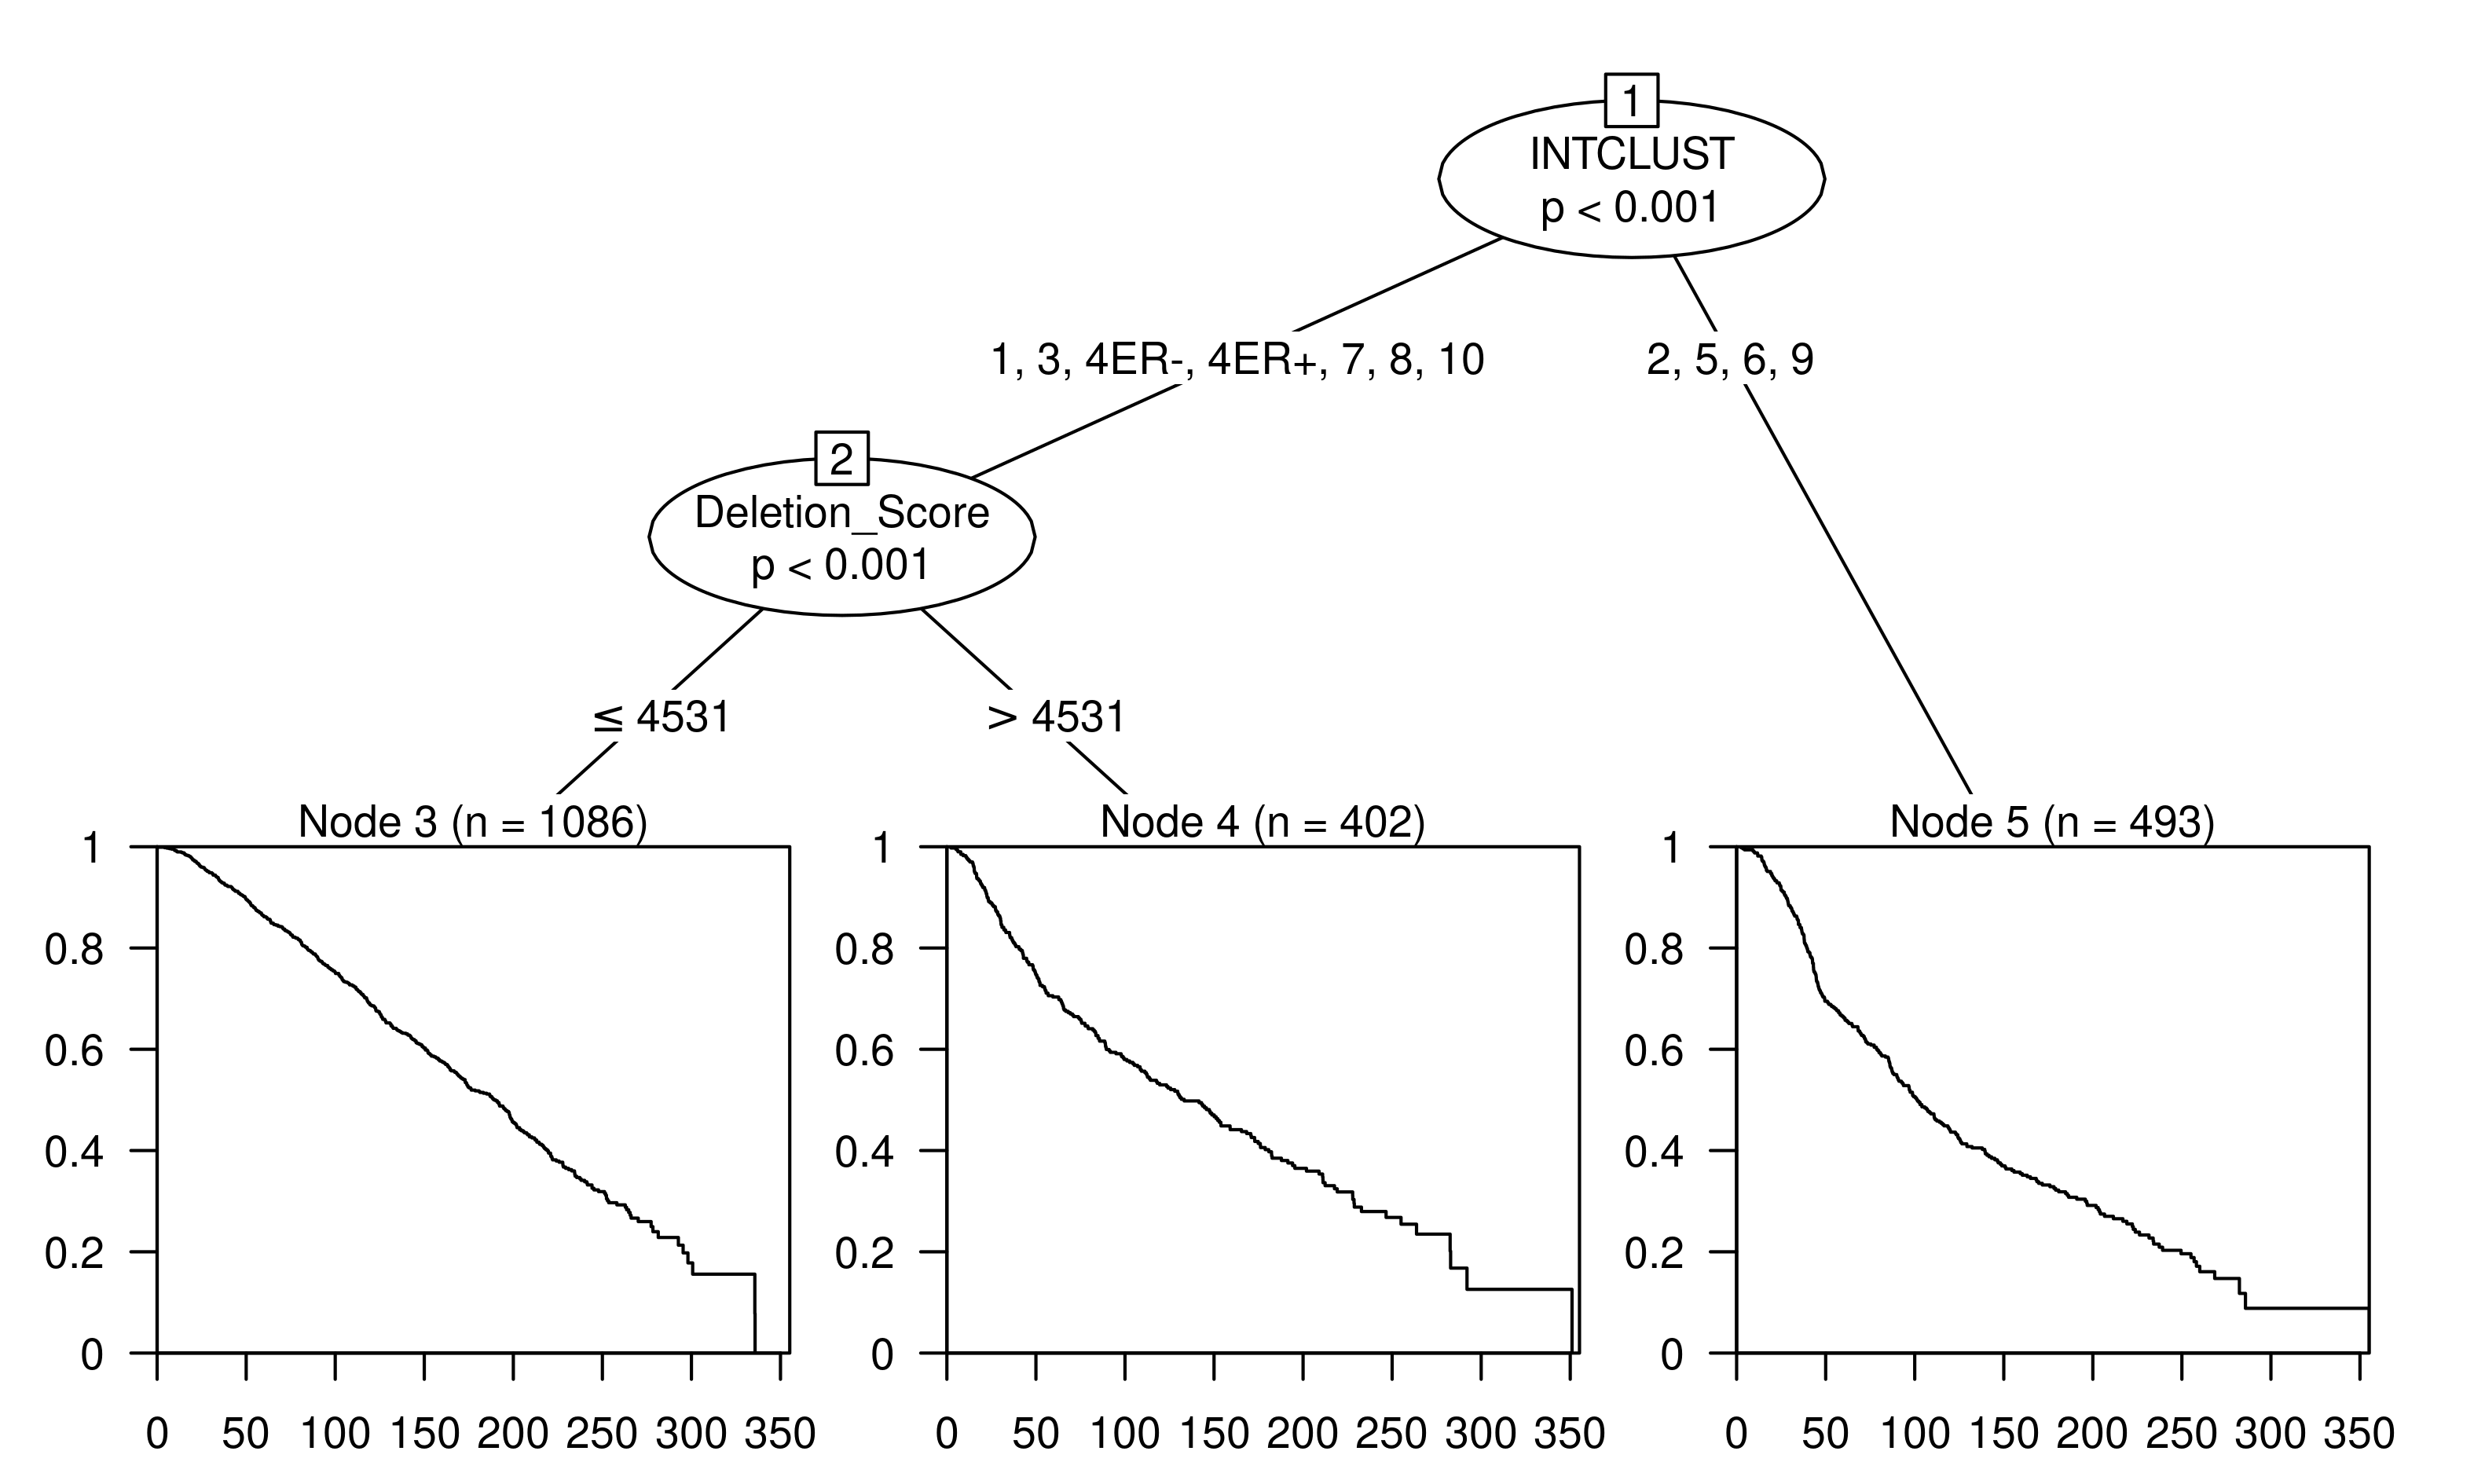
\includegraphics[width=1\textwidth]{../figures/Appendices/Appendix_B/Ctree_Survival_Score_OS_INTCLUST.png}
\end{subfigure}

\vspace{0.5cm}

\caption[Recursive partitioning survival trees for overall survival using IntClust and the six CNA Score metrics as candidate predictors.]{Recursive partitioning survival trees for overall survival using IntClust and the six CNA Score metrics as candidate predictors. (A) Trees fitted using the rpart algorithm and (B) trees fitted using the ctree algorithm.}
\end{figure}

\begin{figure}[!htb]
\centering

\vspace{0.5cm}

\begin{subfigure}{\textwidth}
\subcaption{}
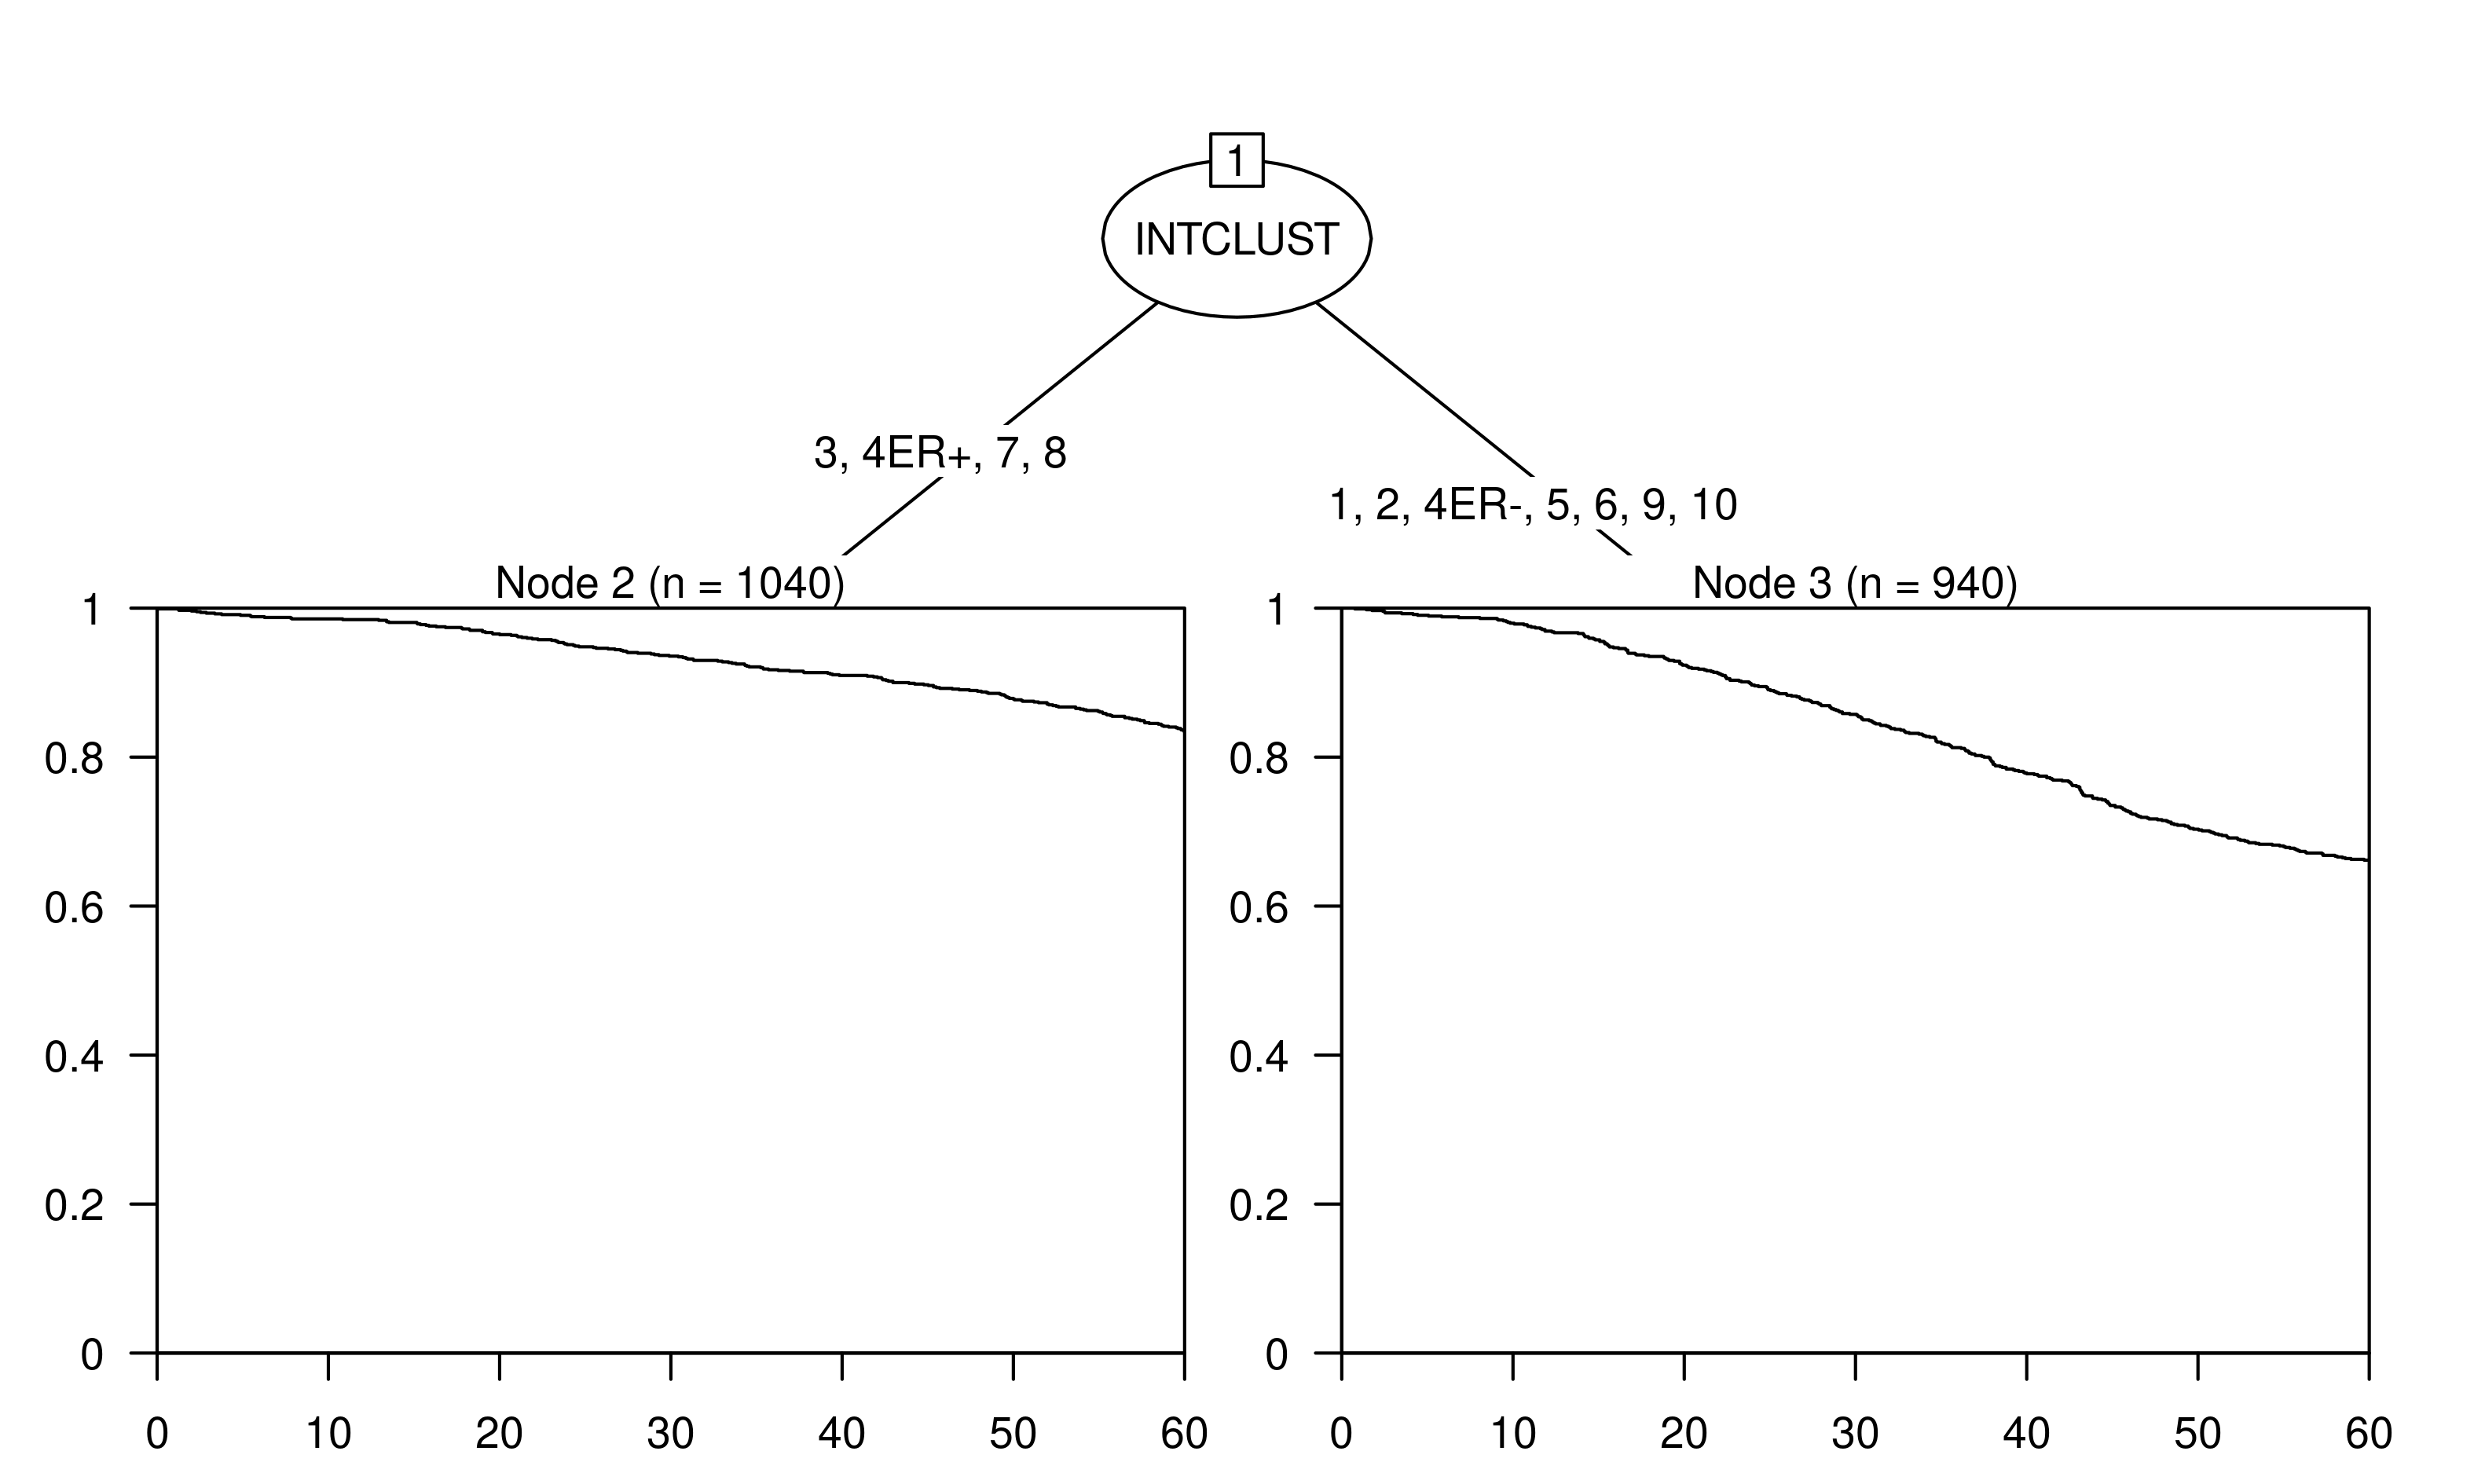
\includegraphics[width=1\textwidth]{../figures/Appendices/Appendix_B/PartyKit_Survival_Score_FiveYearOS_INTCLUST.png}
\end{subfigure}

\vspace{2cm}

\begin{subfigure}{\textwidth}
\subcaption{}
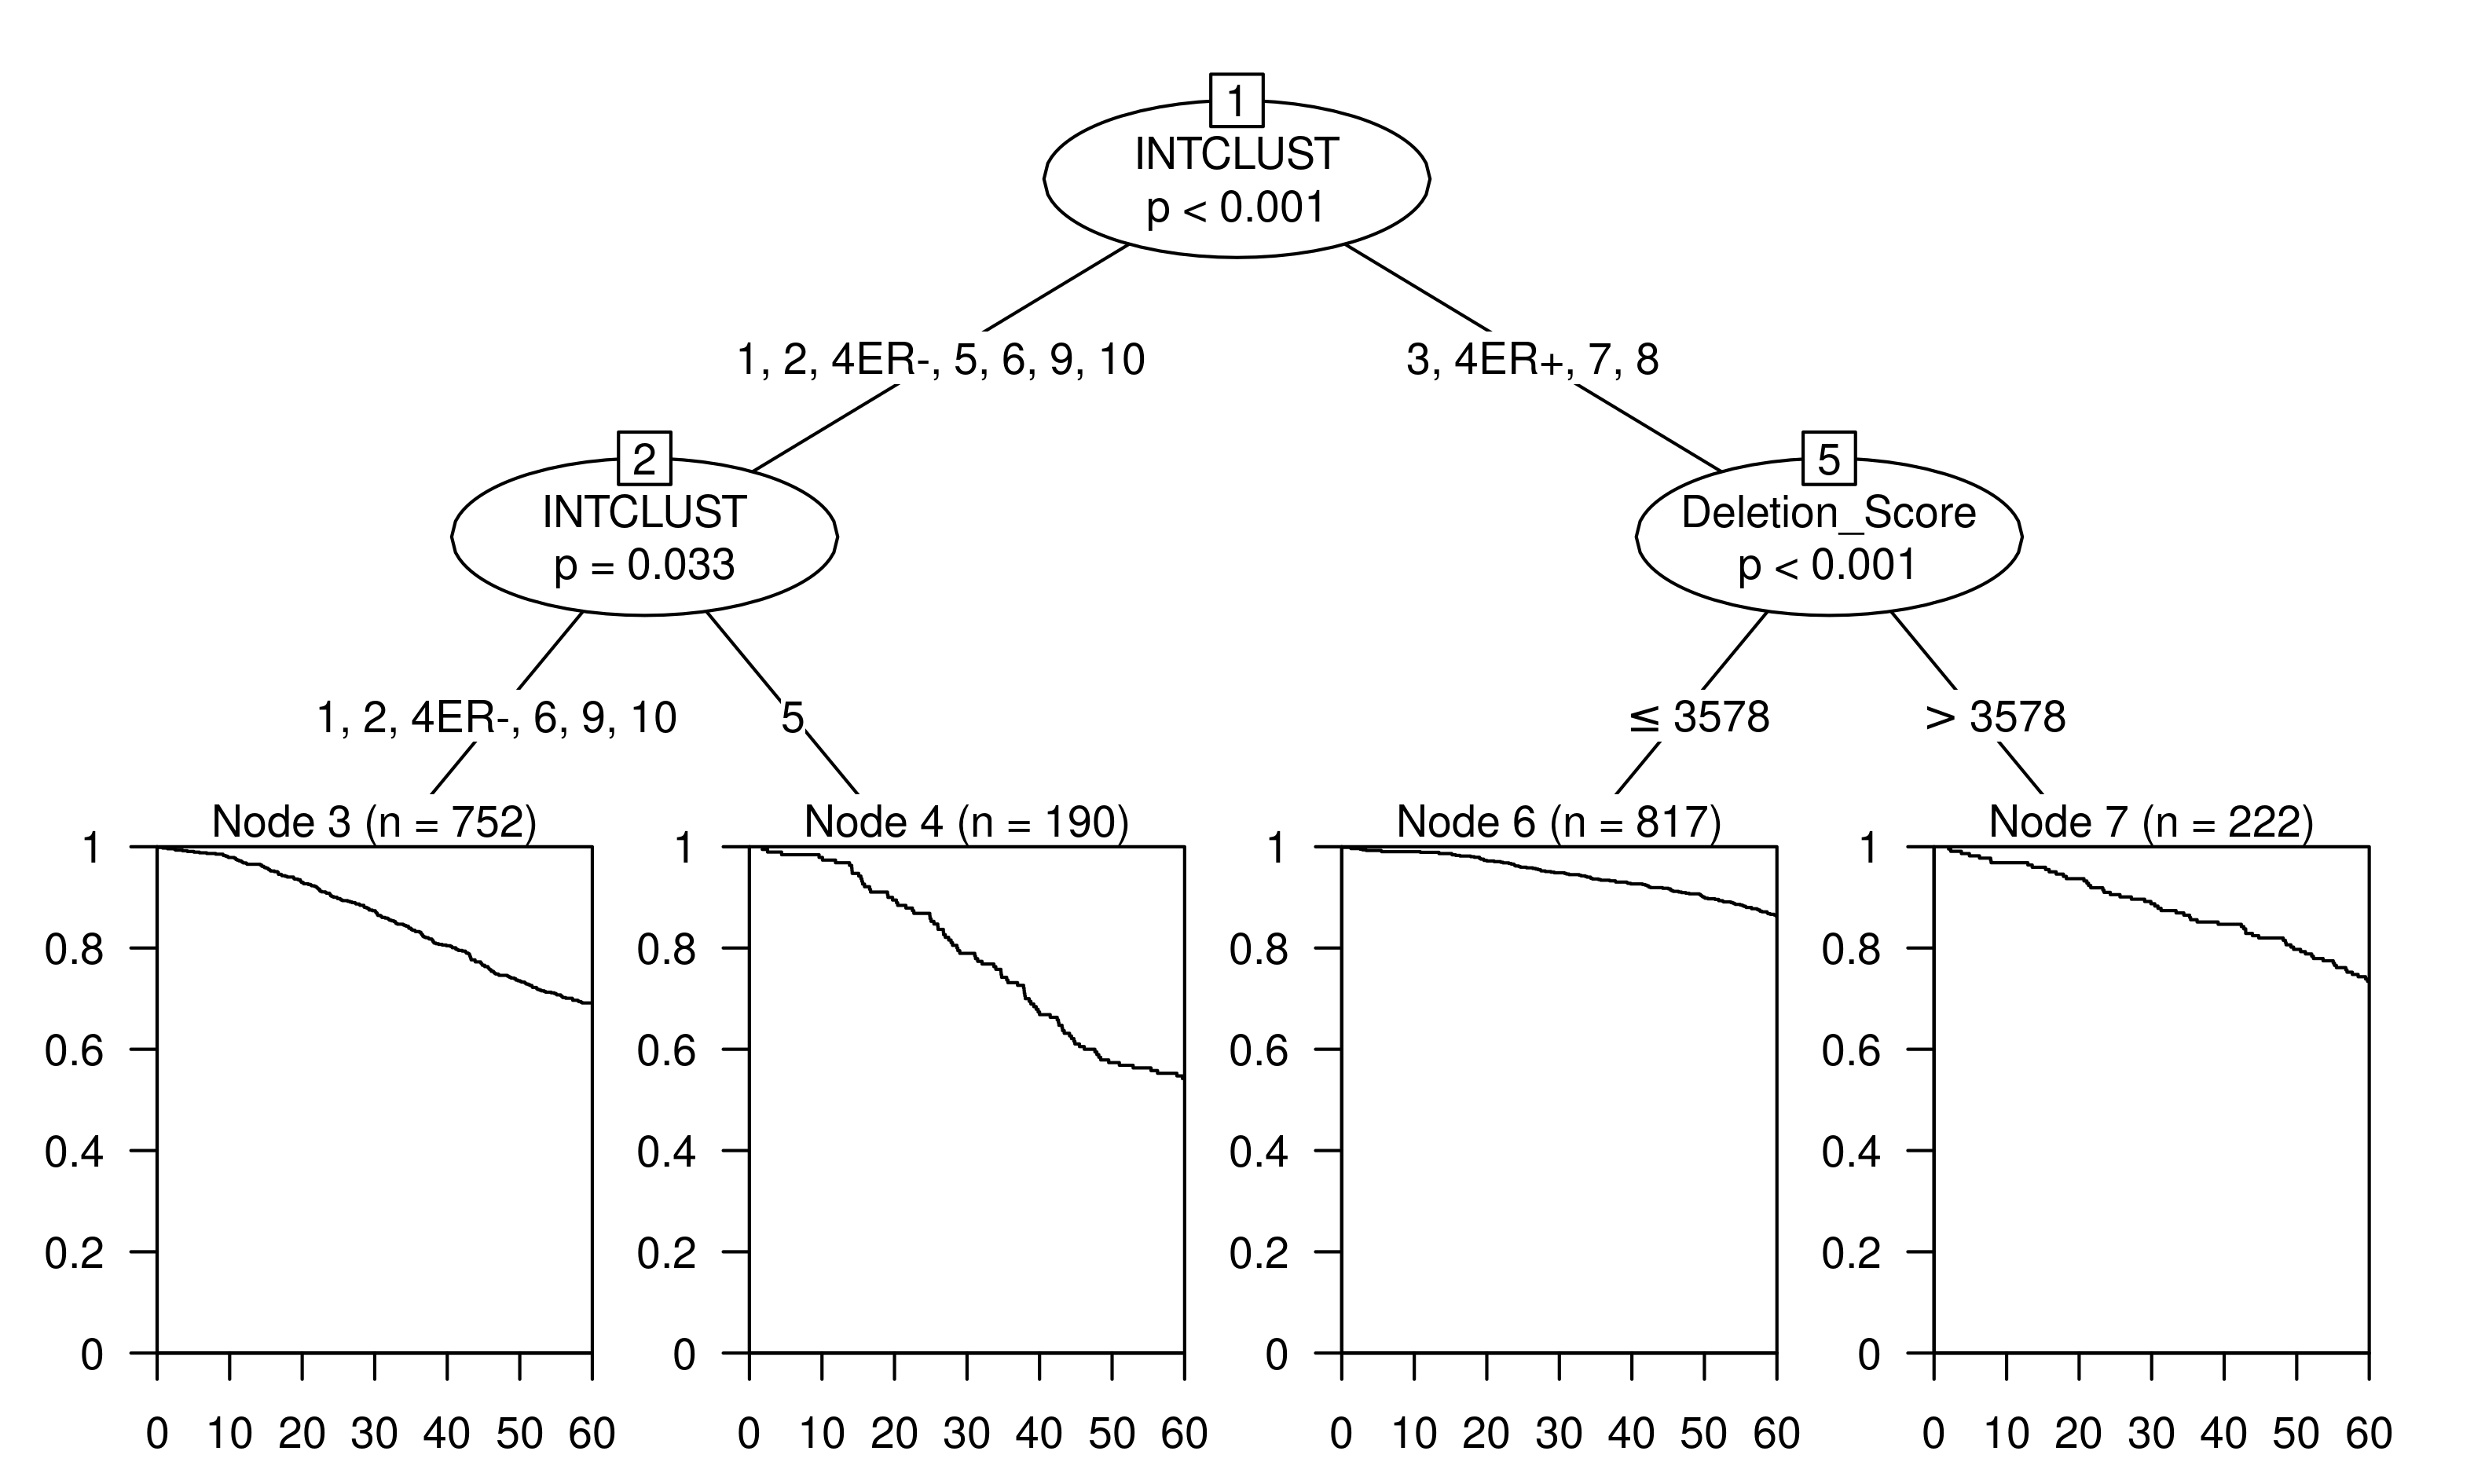
\includegraphics[width=1\textwidth]{../figures/Appendices/Appendix_B/Ctree_Survival_Score_FiveYearOS_INTCLUST.png}
\end{subfigure}

\vspace{0.5cm}

\caption[Recursive partitioning survival trees for five-year overall survival using IntClust and the six CNA Score metrics as candidate predictors.]{Recursive partitioning survival trees for five-year overall survival using IntClust and the six CNA Score metrics as candidate predictors. (A) Trees fitted using the rpart algorithm and (B) trees fitted using the ctree algorithm.}
\end{figure}

\begin{figure}[!htb]
\centering

\vspace{0.5cm}

\begin{subfigure}{\textwidth}
\subcaption{}
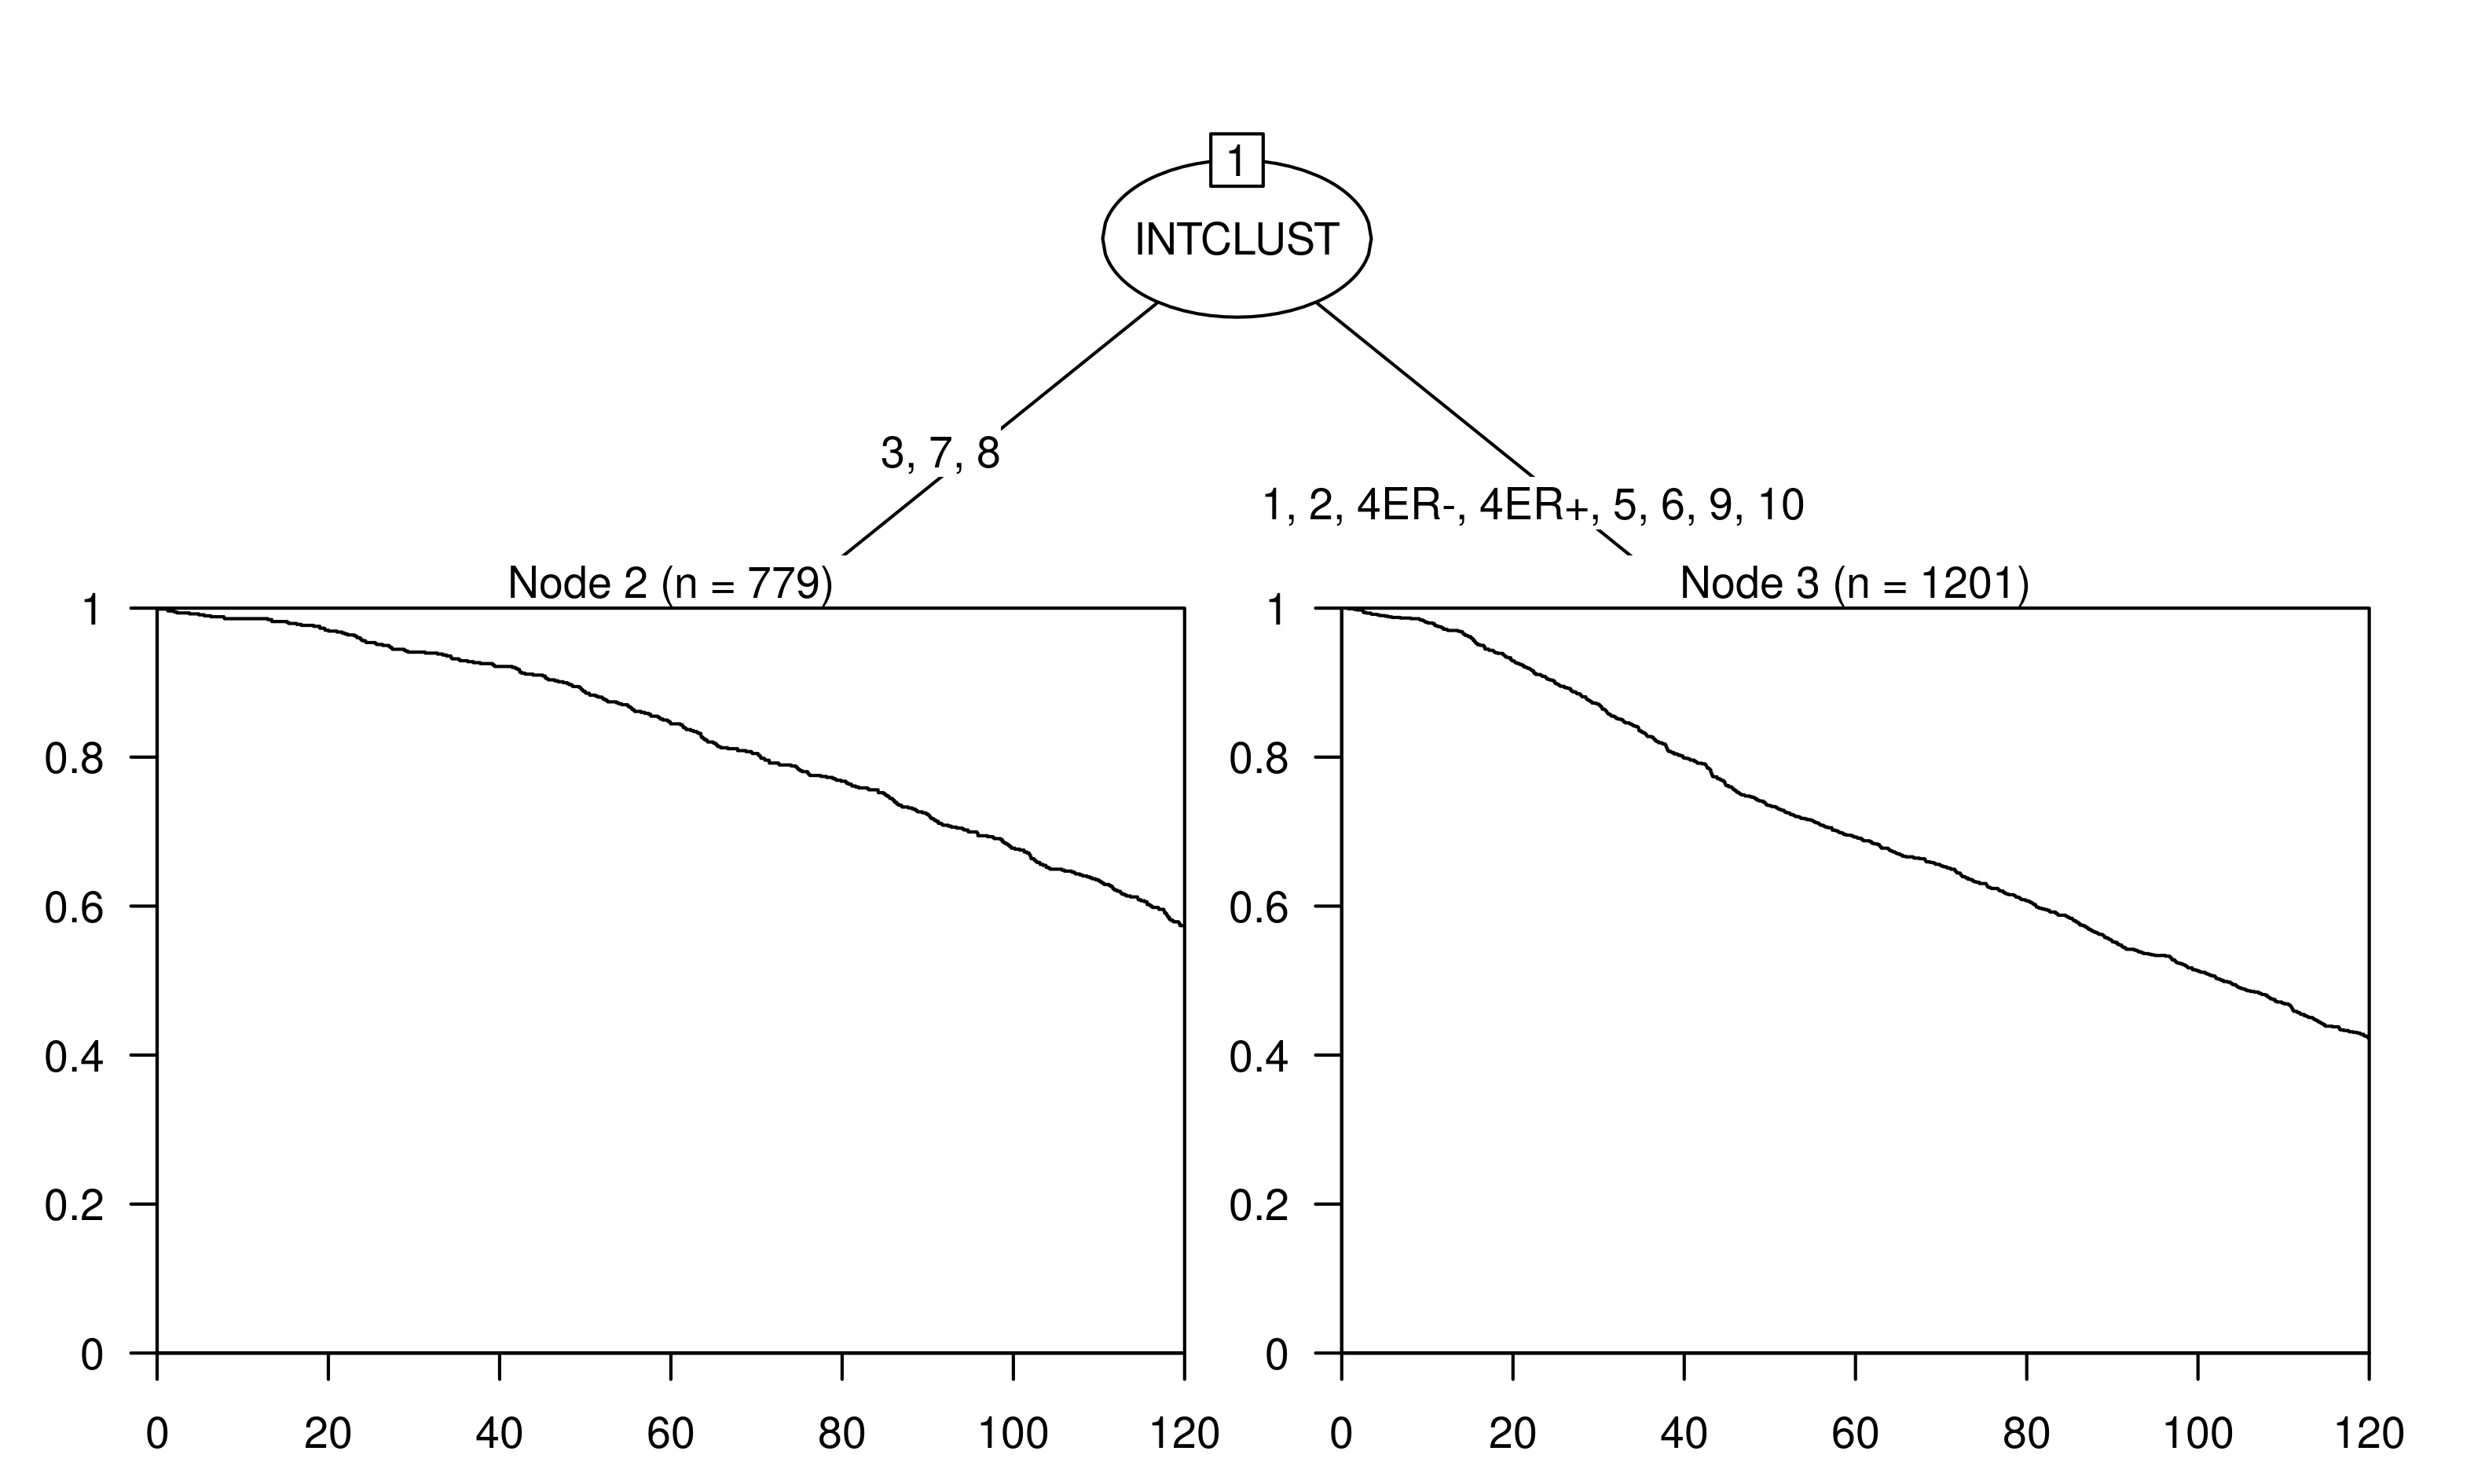
\includegraphics[width=1\textwidth]{../figures/Appendices/Appendix_B/PartyKit_Survival_Score_TenYearOS_INTCLUST.png}
\end{subfigure}

\vspace{2cm}

\begin{subfigure}{\textwidth}
\subcaption{}
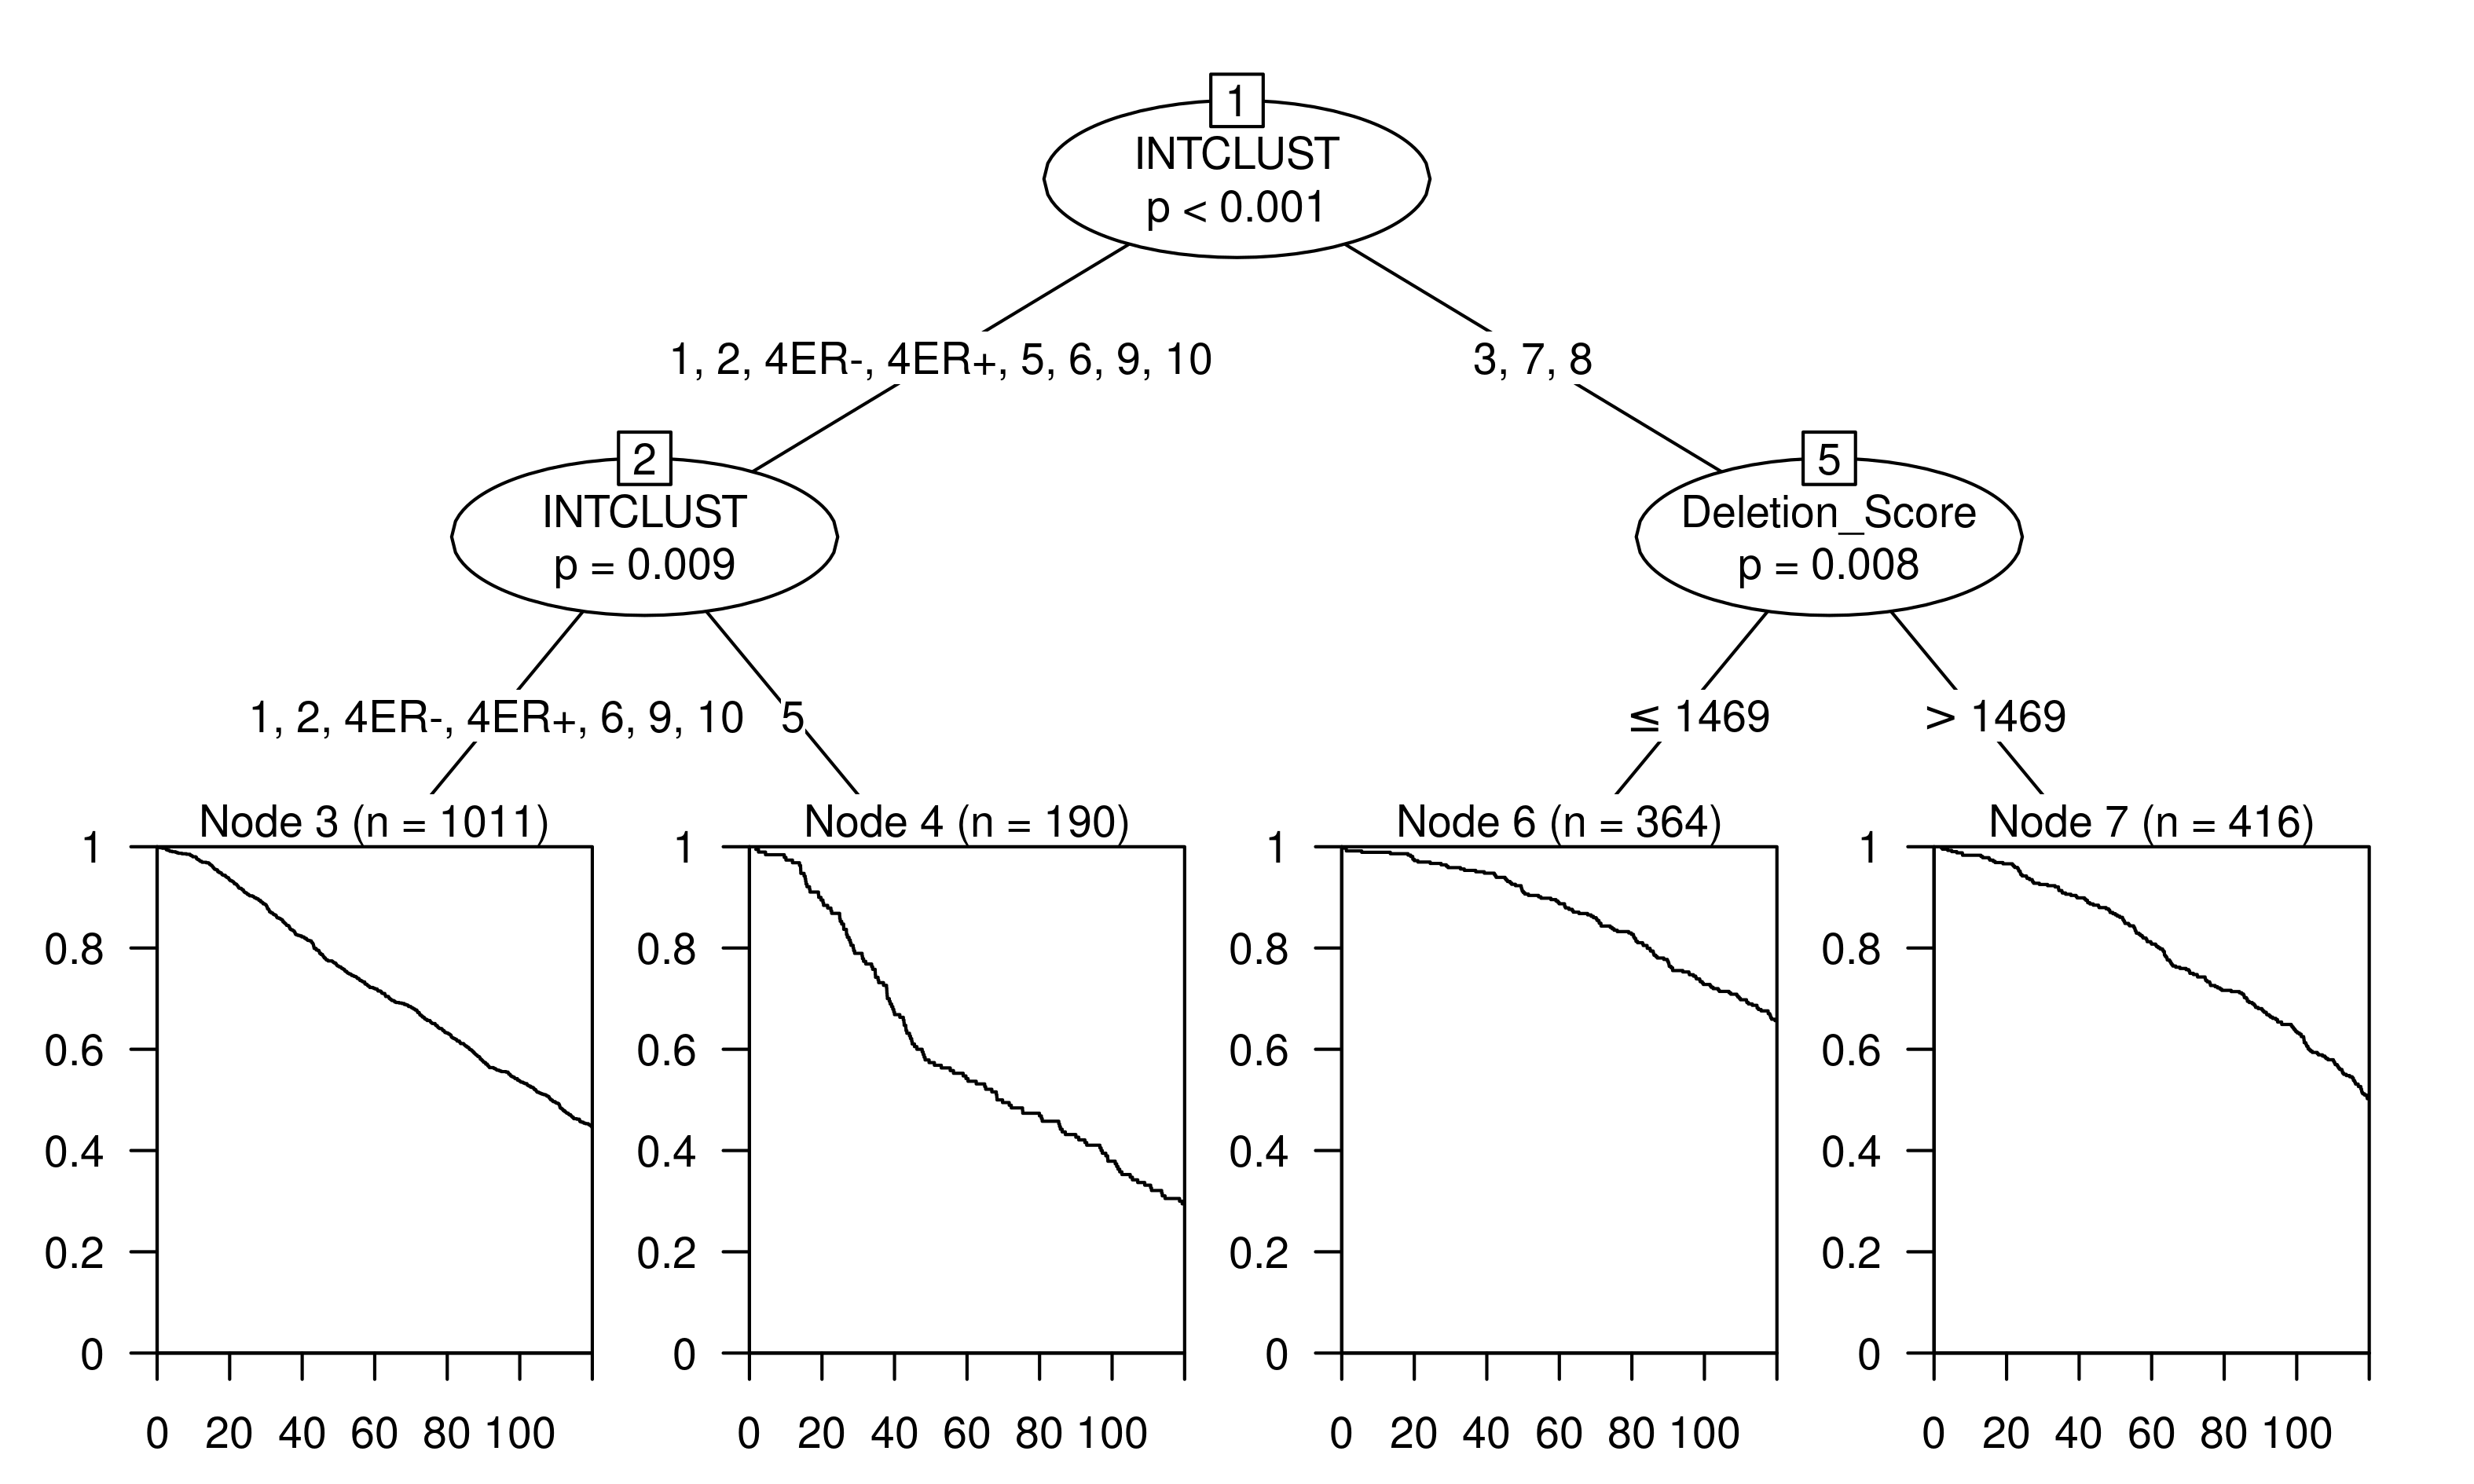
\includegraphics[width=1\textwidth]{../figures/Appendices/Appendix_B/Ctree_Survival_Score_TenYearOS_INTCLUST.png}
\end{subfigure}

\vspace{0.5cm}

\caption[Recursive partitioning survival trees for ten-year overall survival using IntClust and the six CNA Score metrics as candidate predictors.]{Recursive partitioning survival trees for ten-year overall survival using IntClust and the six CNA Score metrics as candidate predictors. (A) Trees fitted using the rpart algorithm and (B) trees fitted using the ctree algorithm.}
\end{figure}

% OS using IntClust and the six CNA Burden metrics as candidate predictors
\begin{figure}[!htb]
\centering

\vspace{0.5cm}

\begin{subfigure}{\textwidth}
\subcaption{}
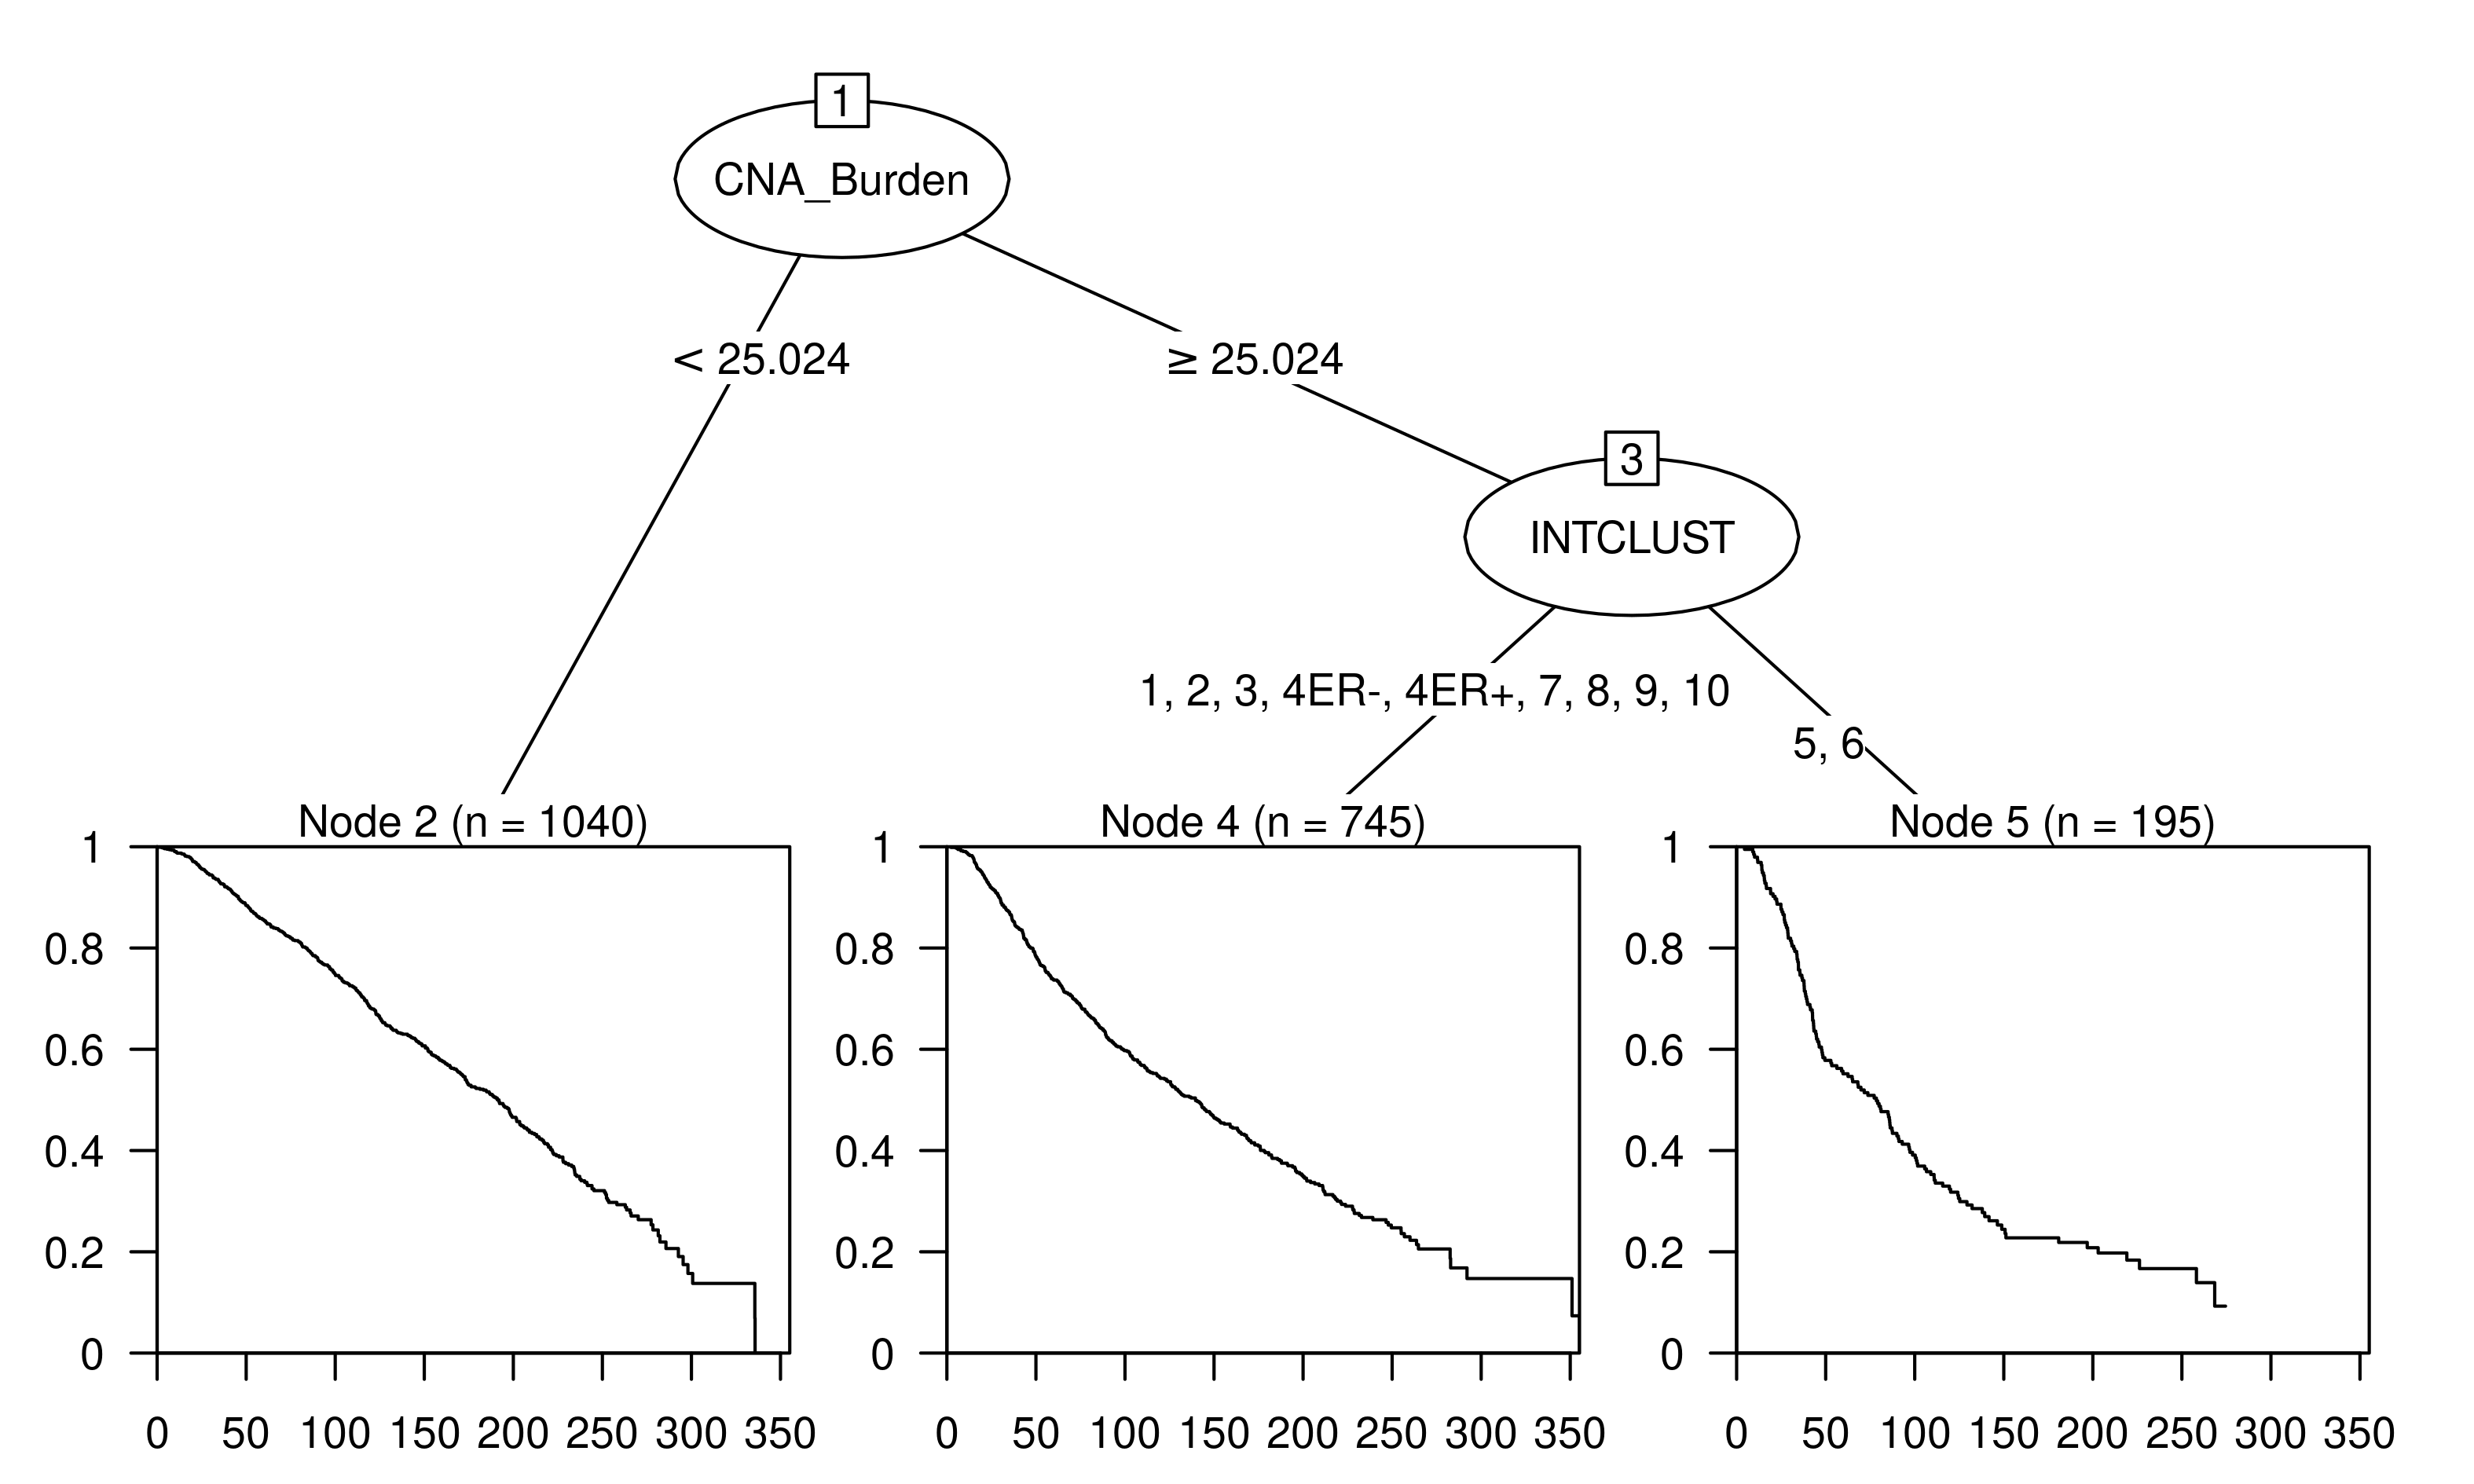
\includegraphics[width=1\textwidth]{../figures/Appendices/Appendix_B/PartyKit_Survival_Burden_OS_INTCLUST.png}
\end{subfigure}

\vspace{2cm}

\begin{subfigure}{\textwidth}
\subcaption{}
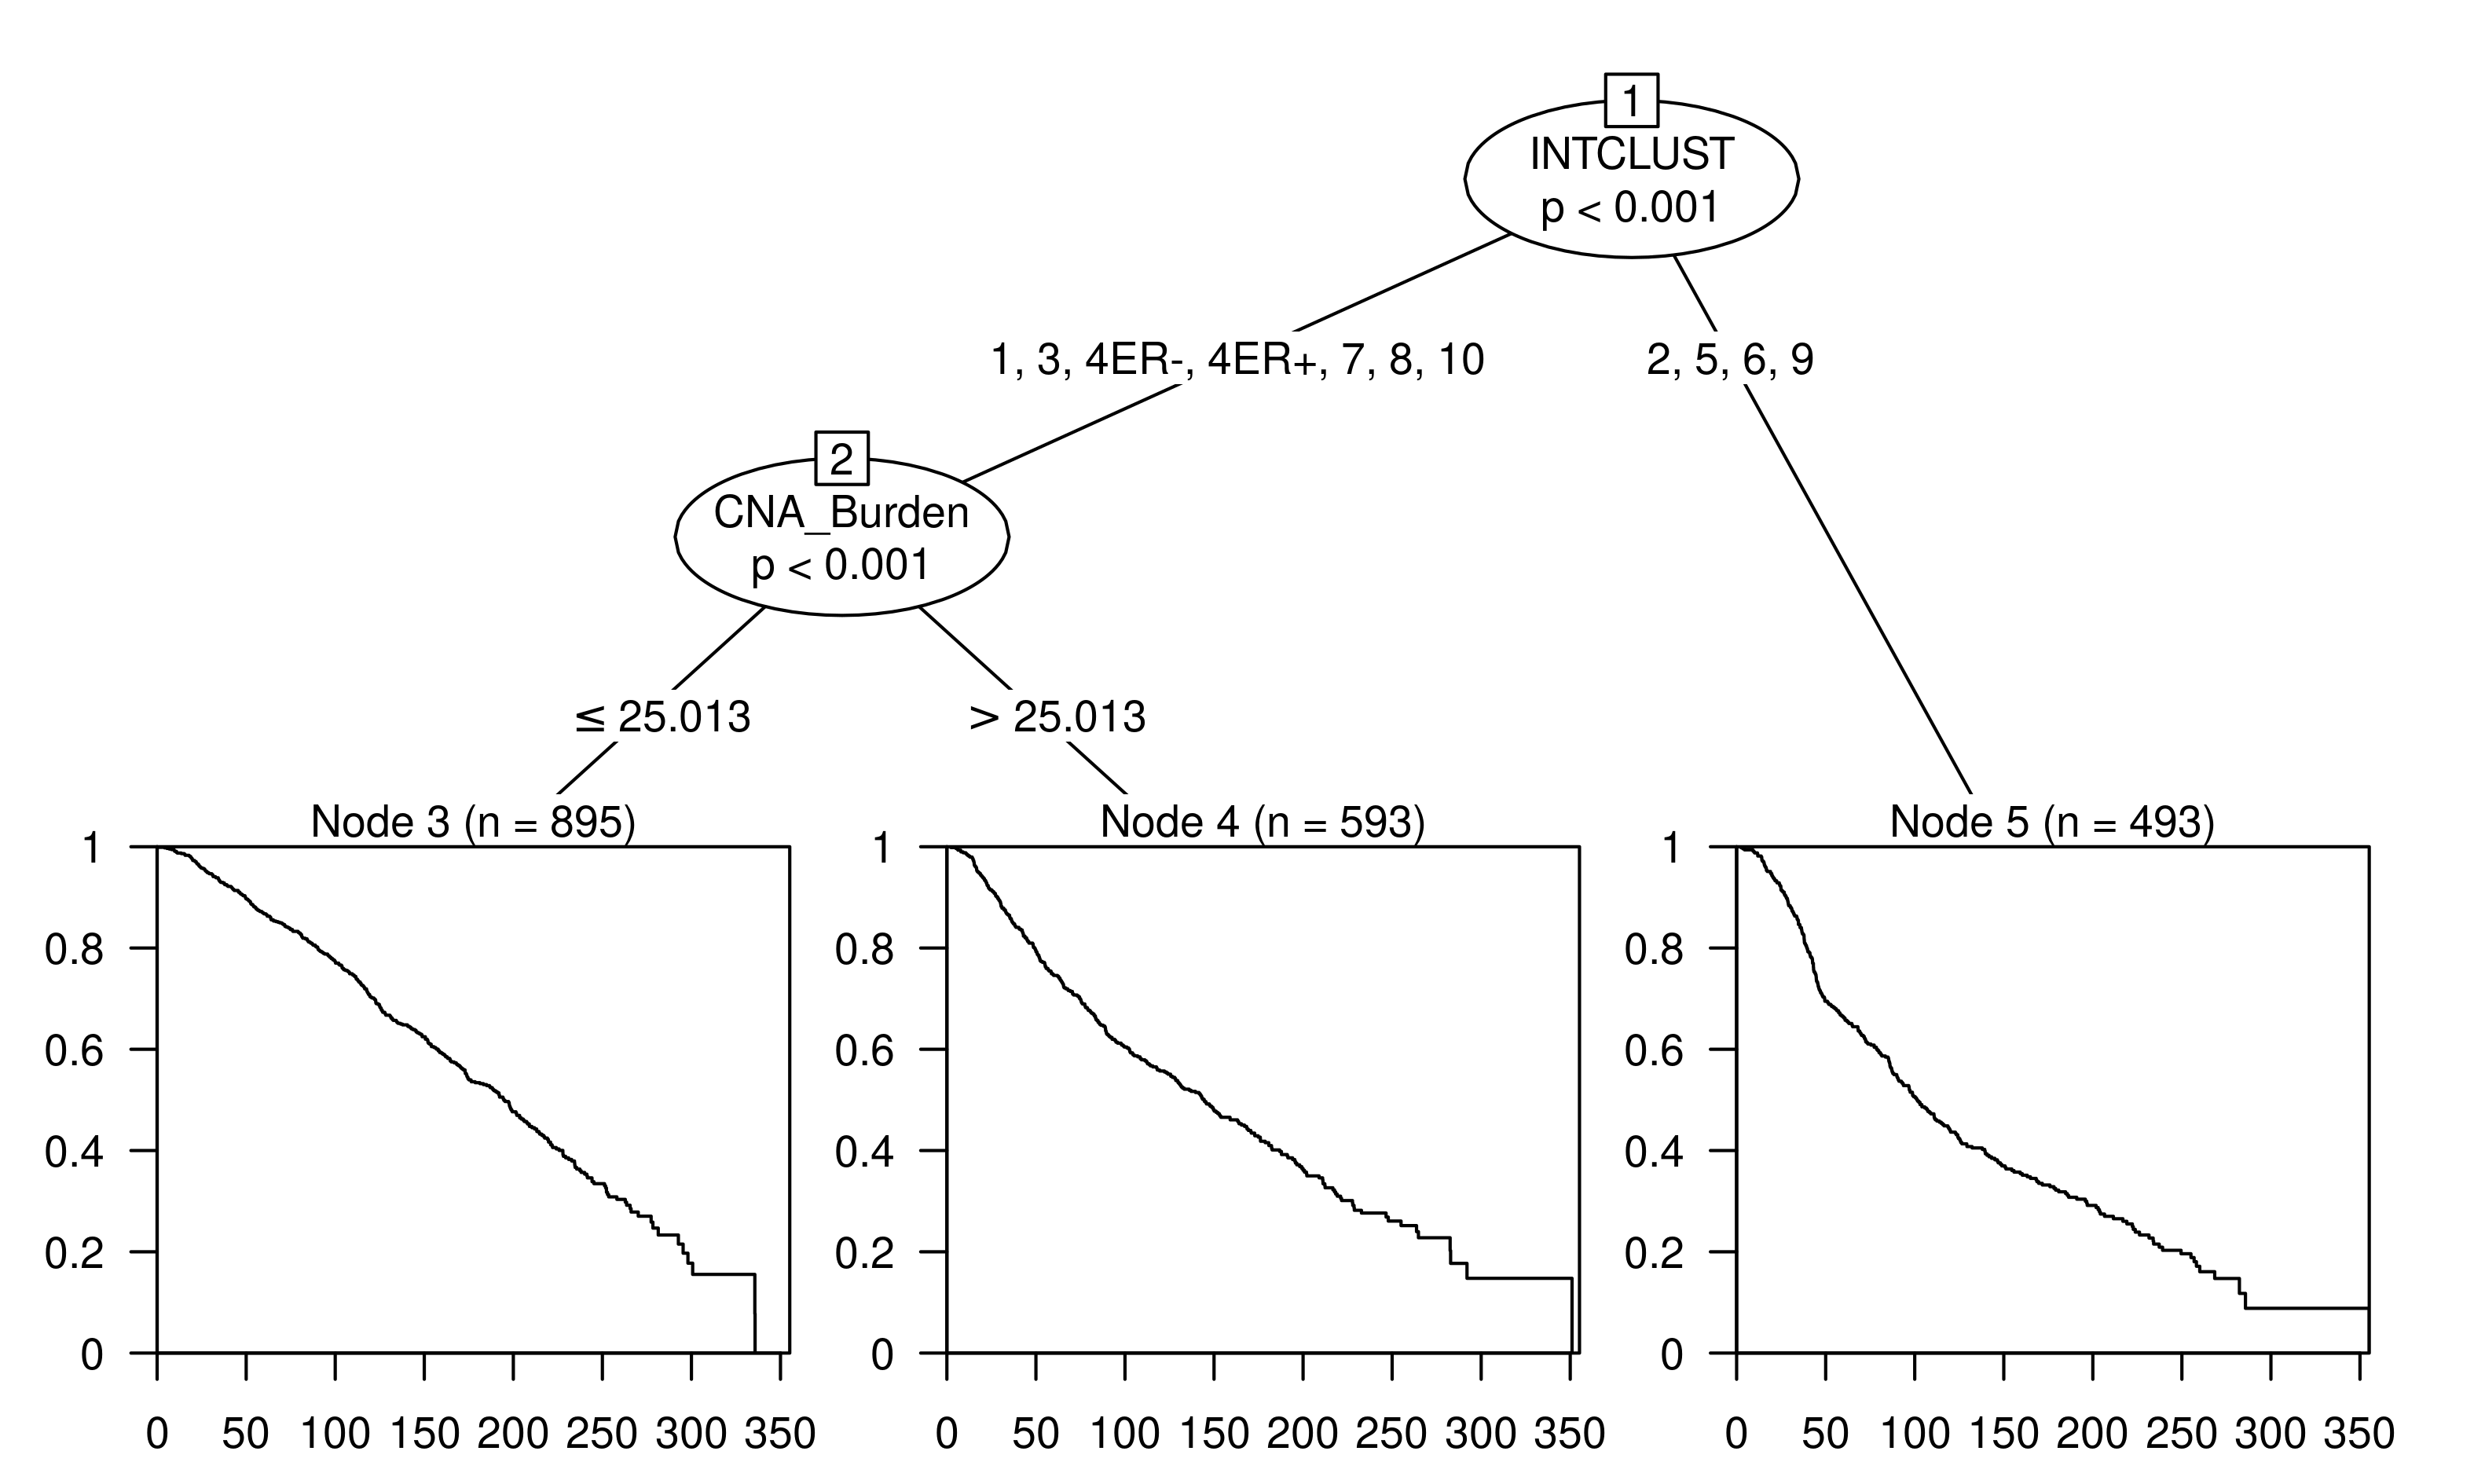
\includegraphics[width=1\textwidth]{../figures/Appendices/Appendix_B/Ctree_Survival_Burden_OS_INTCLUST.png}
\end{subfigure}

\vspace{0.5cm}

\caption[Recursive partitioning survival trees for overall survival using IntClust and the six CNA Burden metrics as candidate predictors.]{Recursive partitioning survival trees for overall survival using IntClust and the six CNA Burden metrics as candidate predictors. (A) Trees fitted using the rpart algorithm and (B) trees fitted using the ctree algorithm.}
\end{figure}

\begin{figure}[!htb]
\centering

\vspace{0.5cm}

\begin{subfigure}{\textwidth}
\subcaption{}
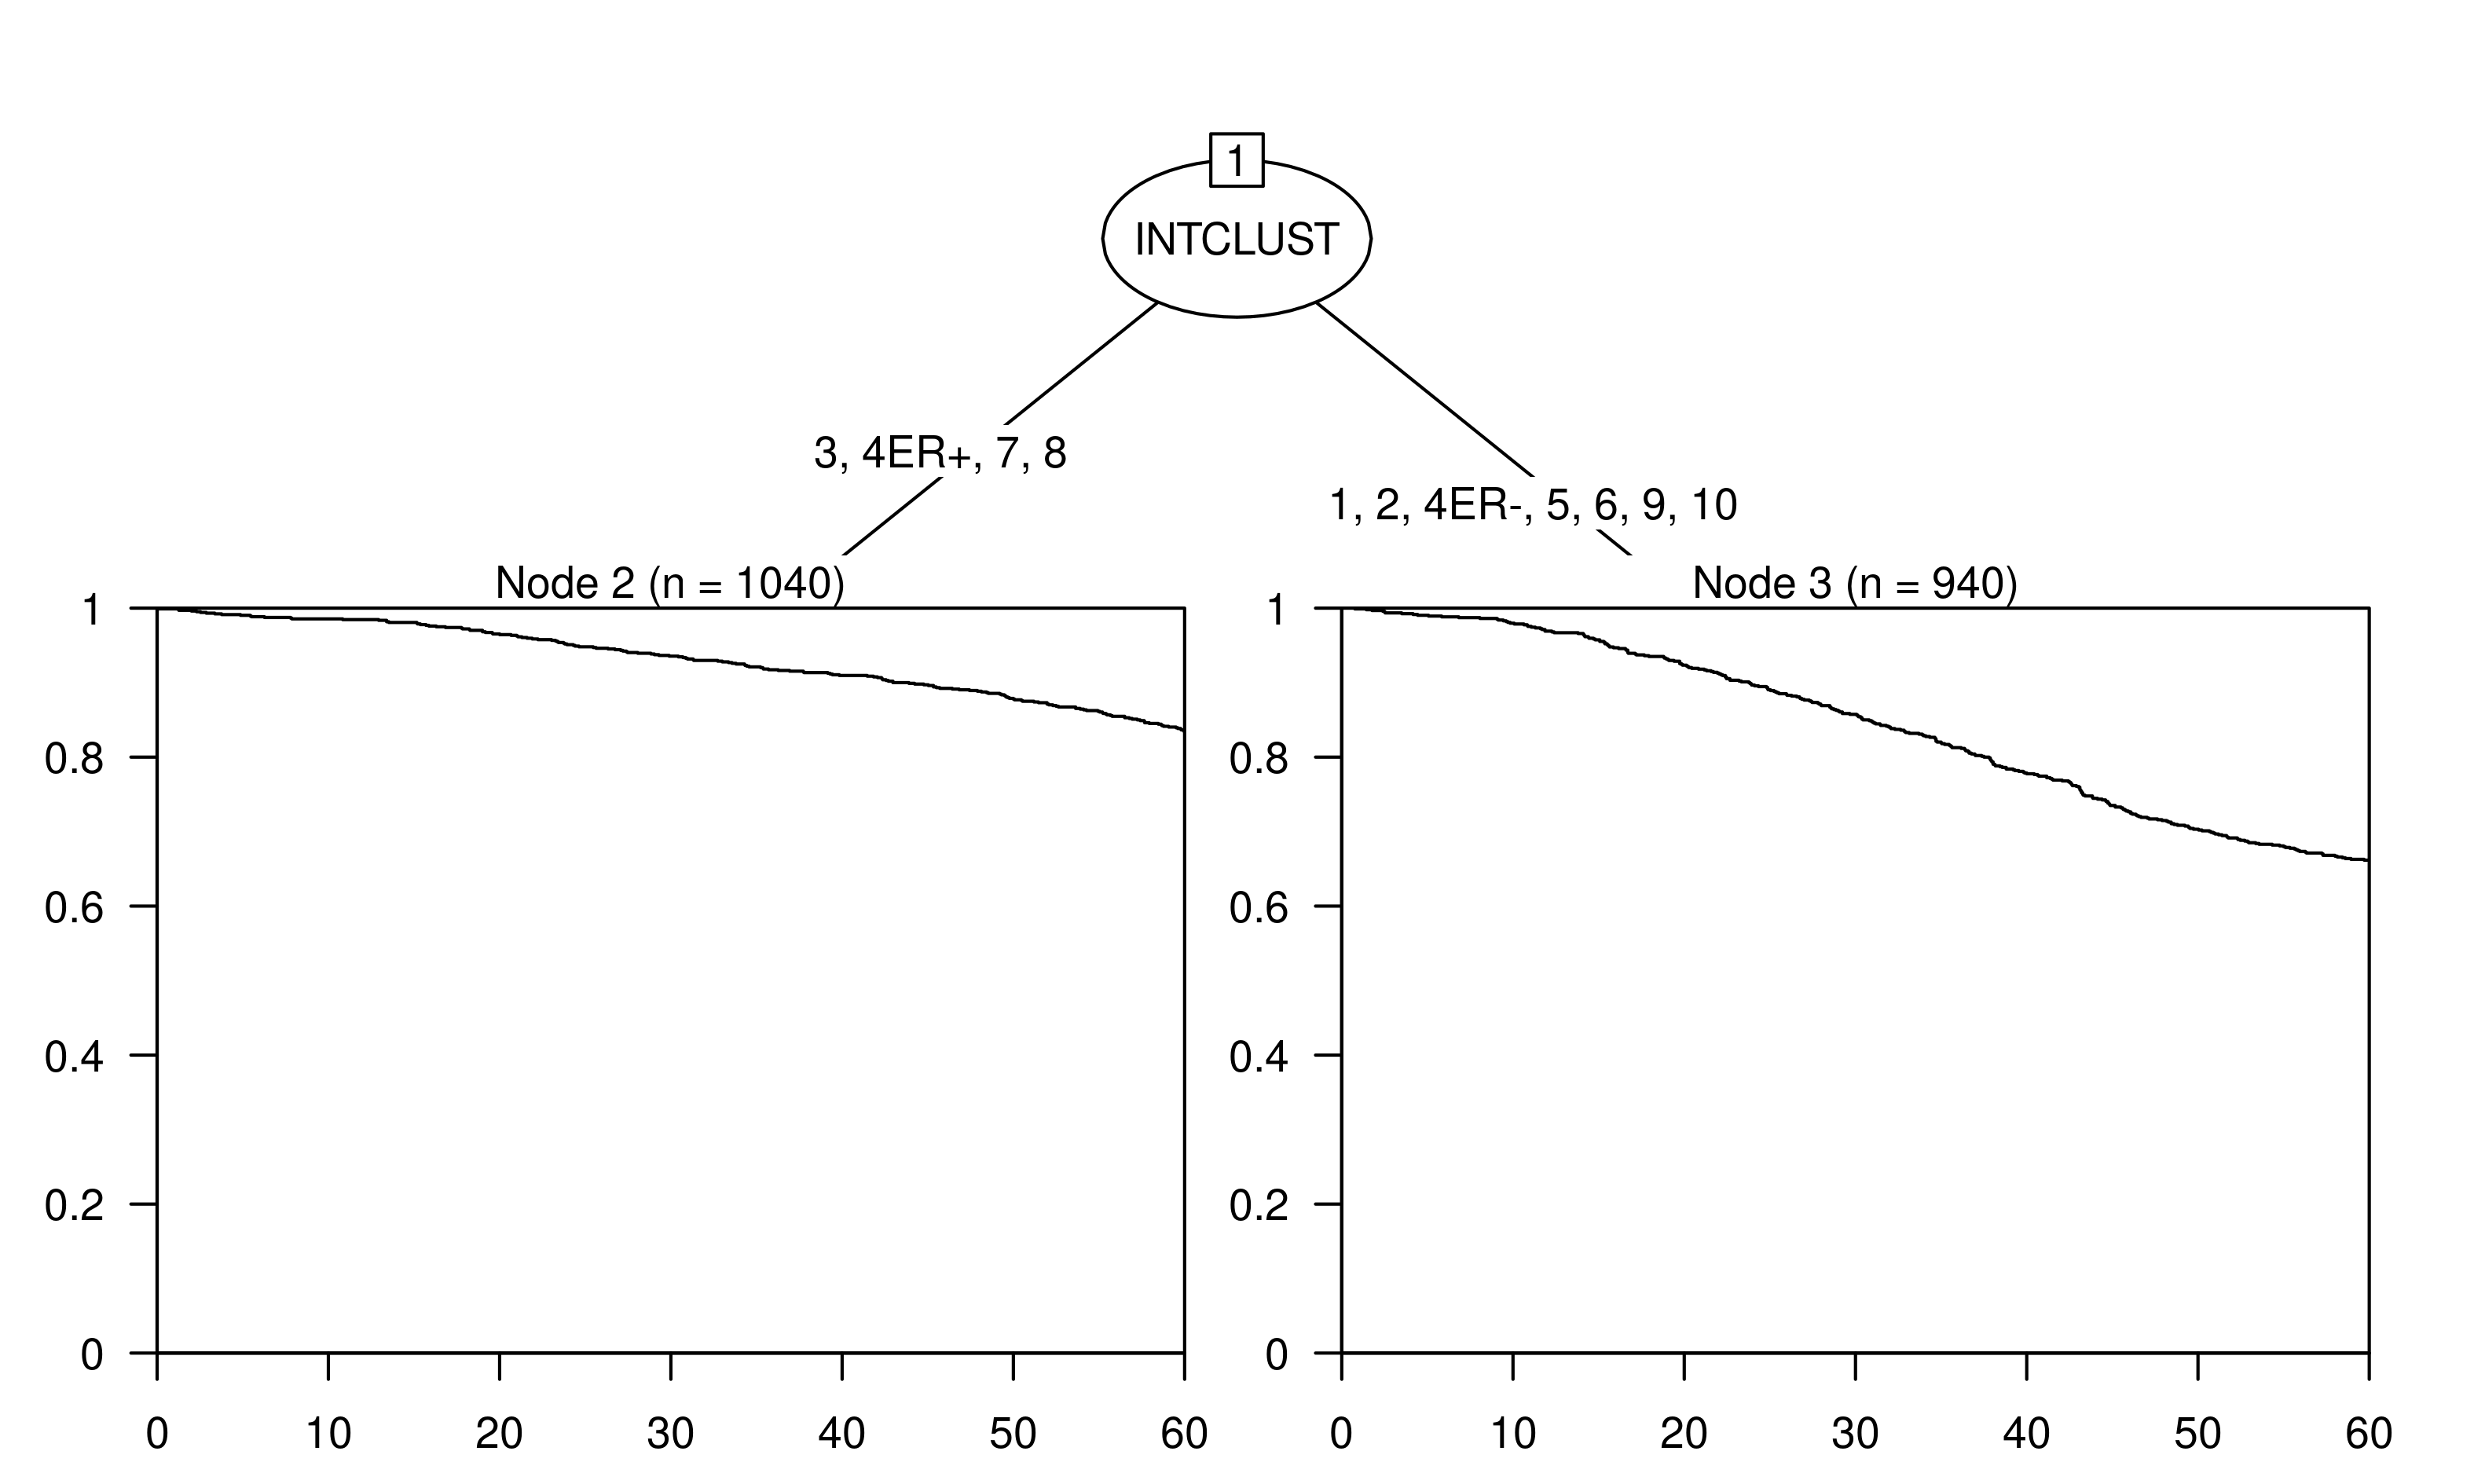
\includegraphics[width=1\textwidth]{../figures/Appendices/Appendix_B/PartyKit_Survival_Burden_FiveYearOS_INTCLUST.png}
\end{subfigure}

\vspace{2cm}

\begin{subfigure}{\textwidth}
\subcaption{}
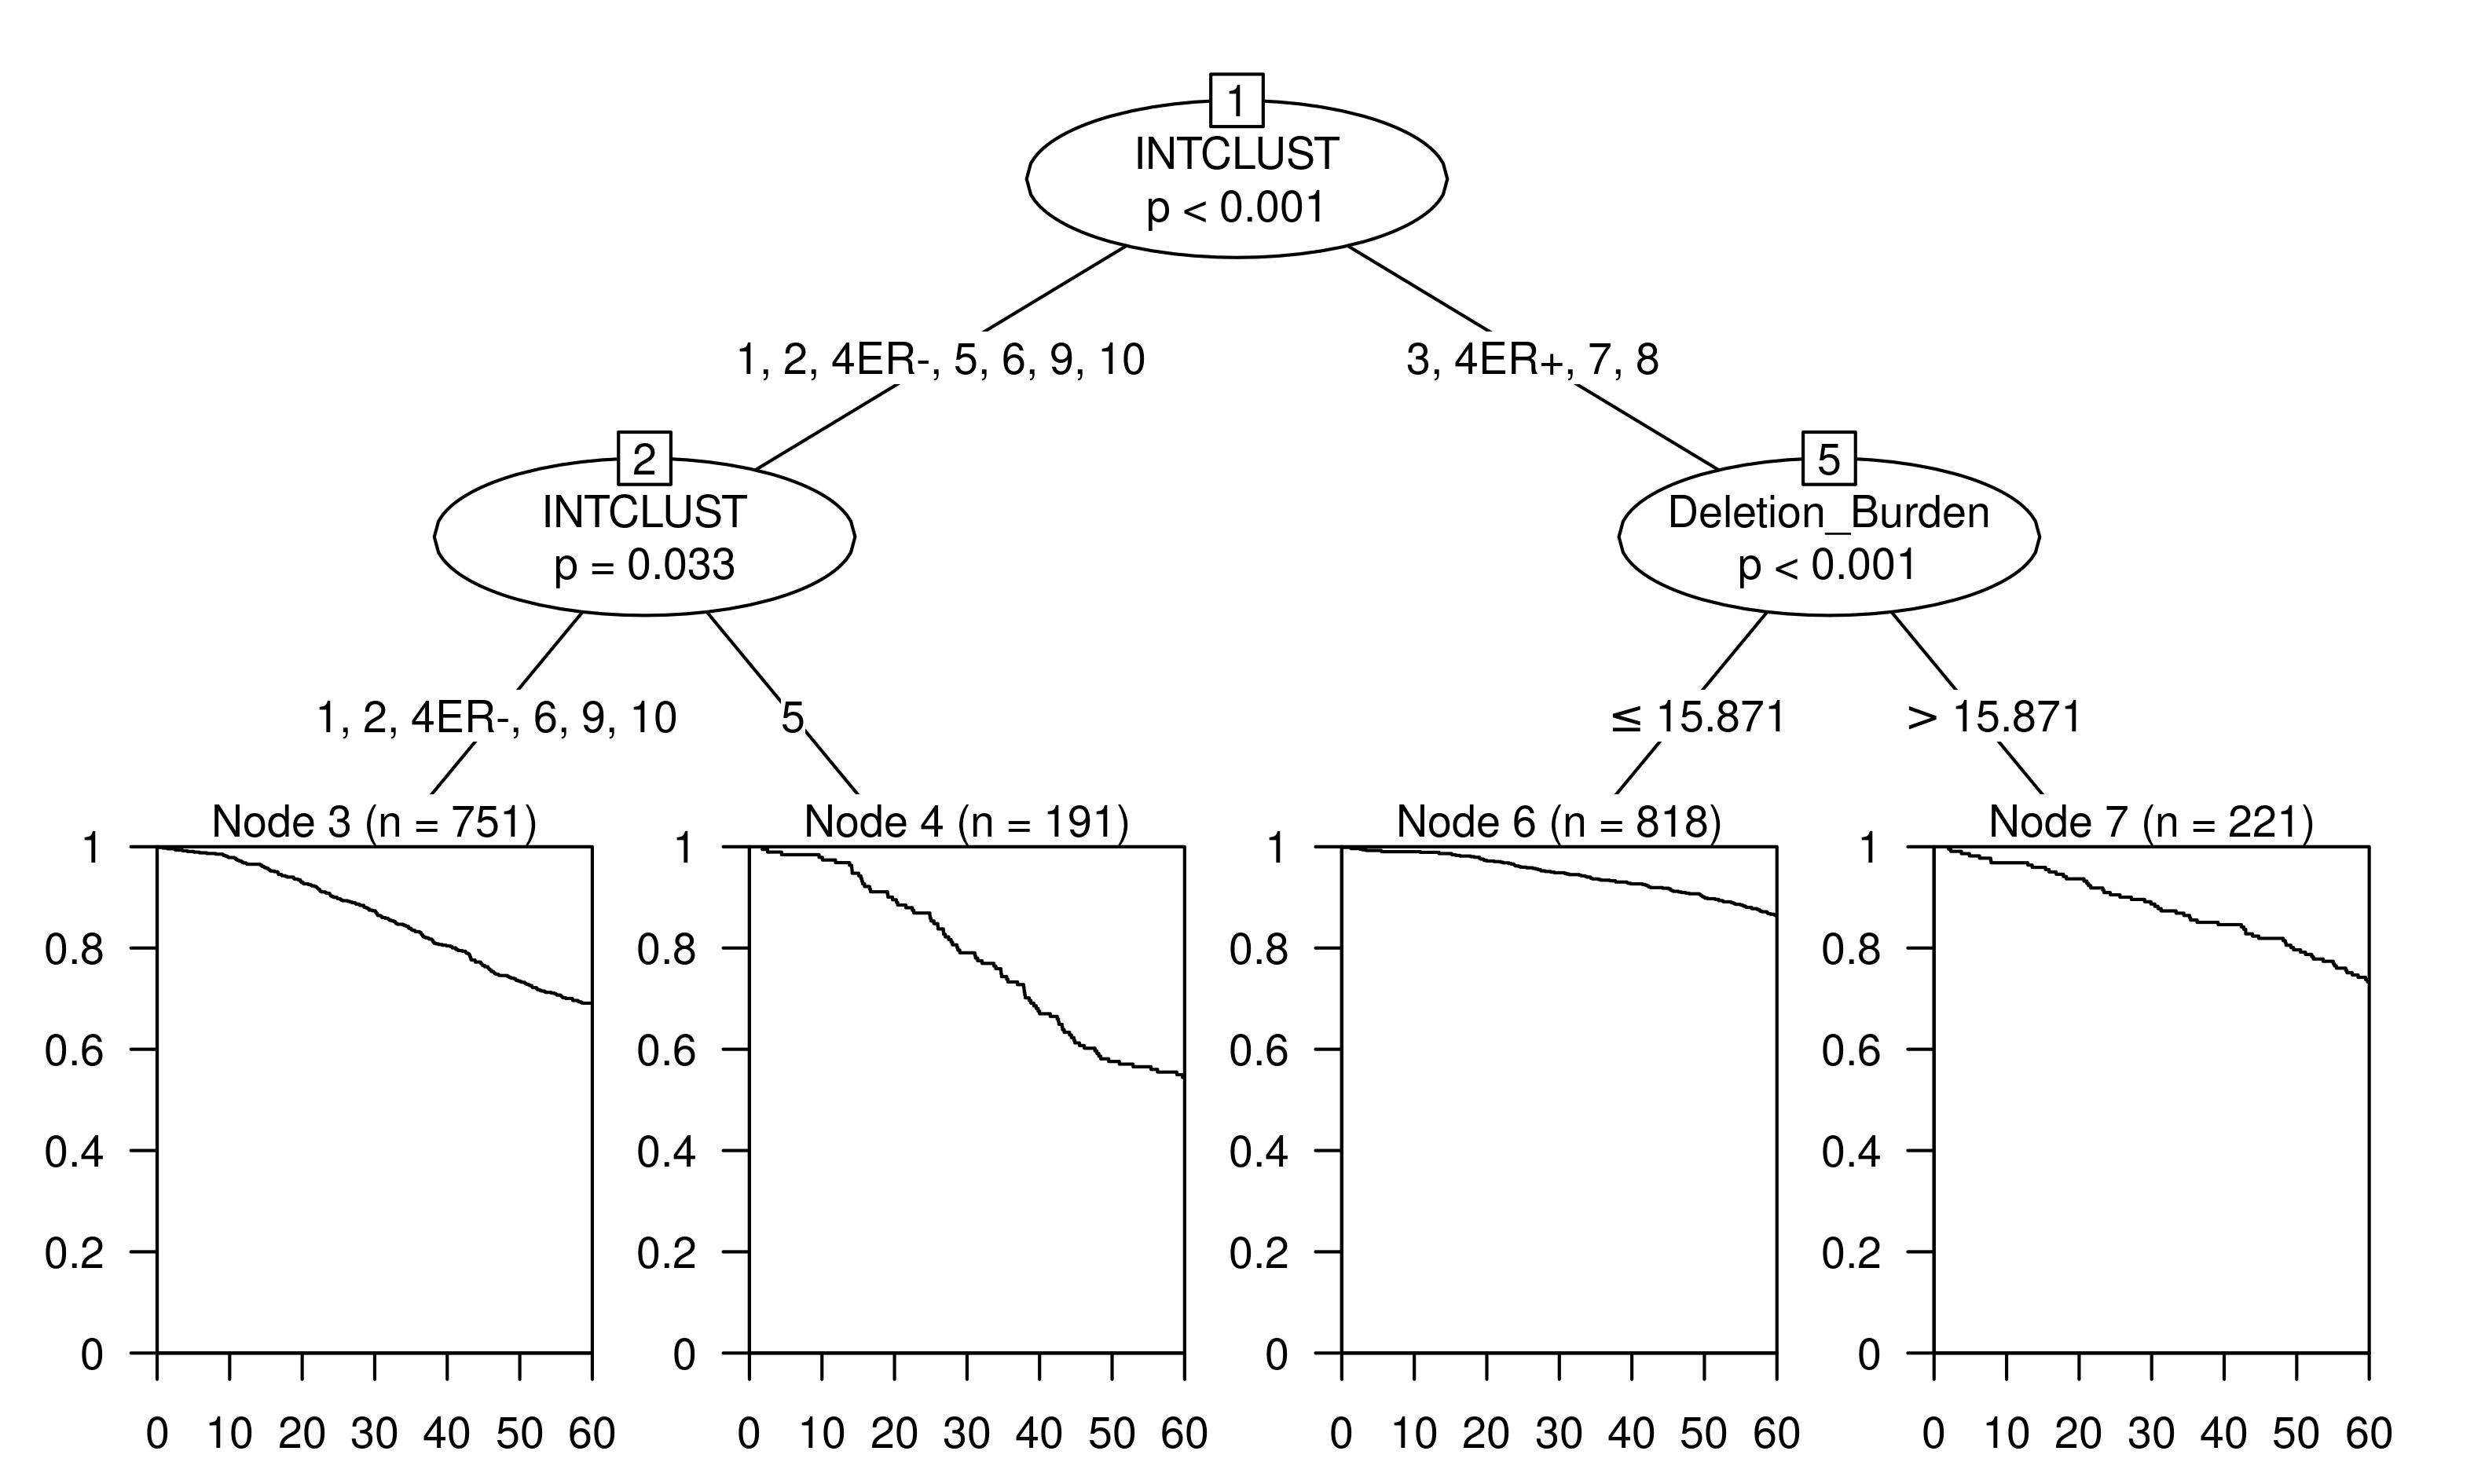
\includegraphics[width=1\textwidth]{../figures/Appendices/Appendix_B/Ctree_Survival_Burden_FiveYearOS_INTCLUST.png}
\end{subfigure}

\vspace{0.5cm}

\caption[Recursive partitioning survival trees for five-year overall survival using IntClust and the six CNA Burden metrics as candidate predictors.]{Recursive partitioning survival trees for five-year overall survival using IntClust and the six CNA Burden metrics as candidate predictors. (A) Trees fitted using the rpart algorithm and (B) trees fitted using the ctree algorithm.}
\end{figure}

\begin{figure}[!htb]
\centering

\vspace{0.5cm}

\begin{subfigure}{\textwidth}
\subcaption{}
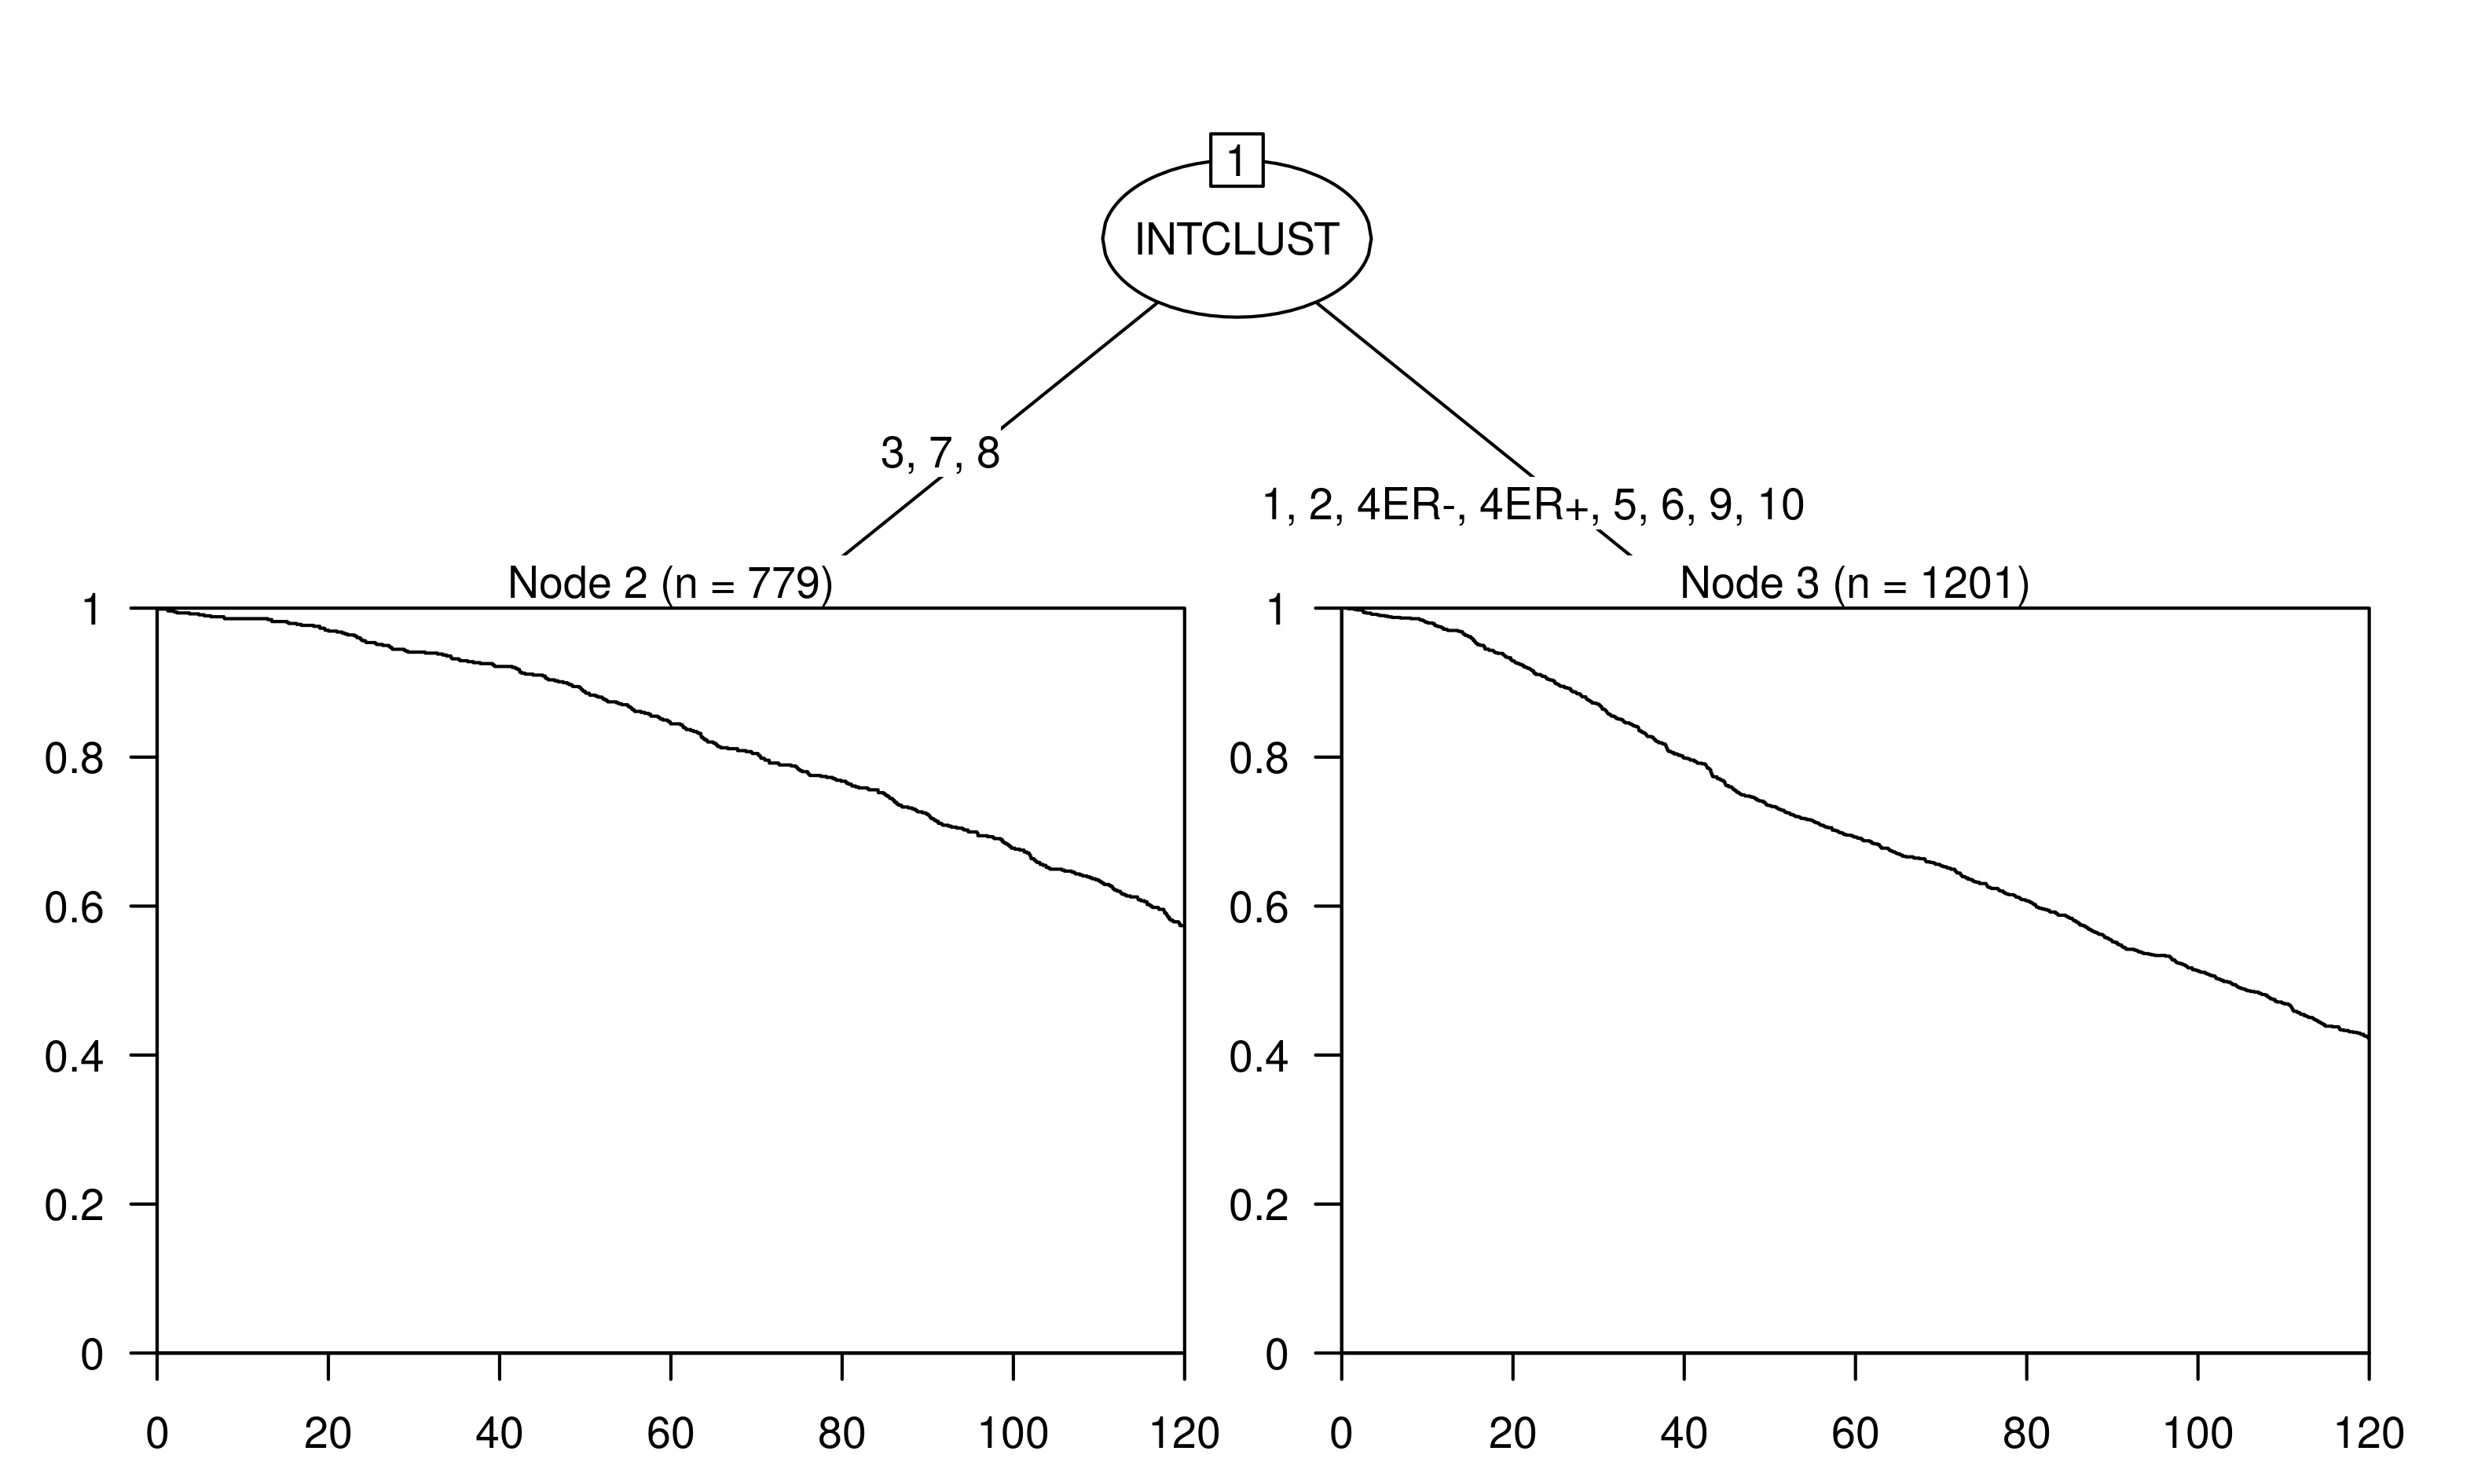
\includegraphics[width=1\textwidth]{../figures/Appendices/Appendix_B/PartyKit_Survival_Burden_TenYearOS_INTCLUST.png}
\end{subfigure}

\vspace{2cm}

\begin{subfigure}{\textwidth}
\subcaption{}
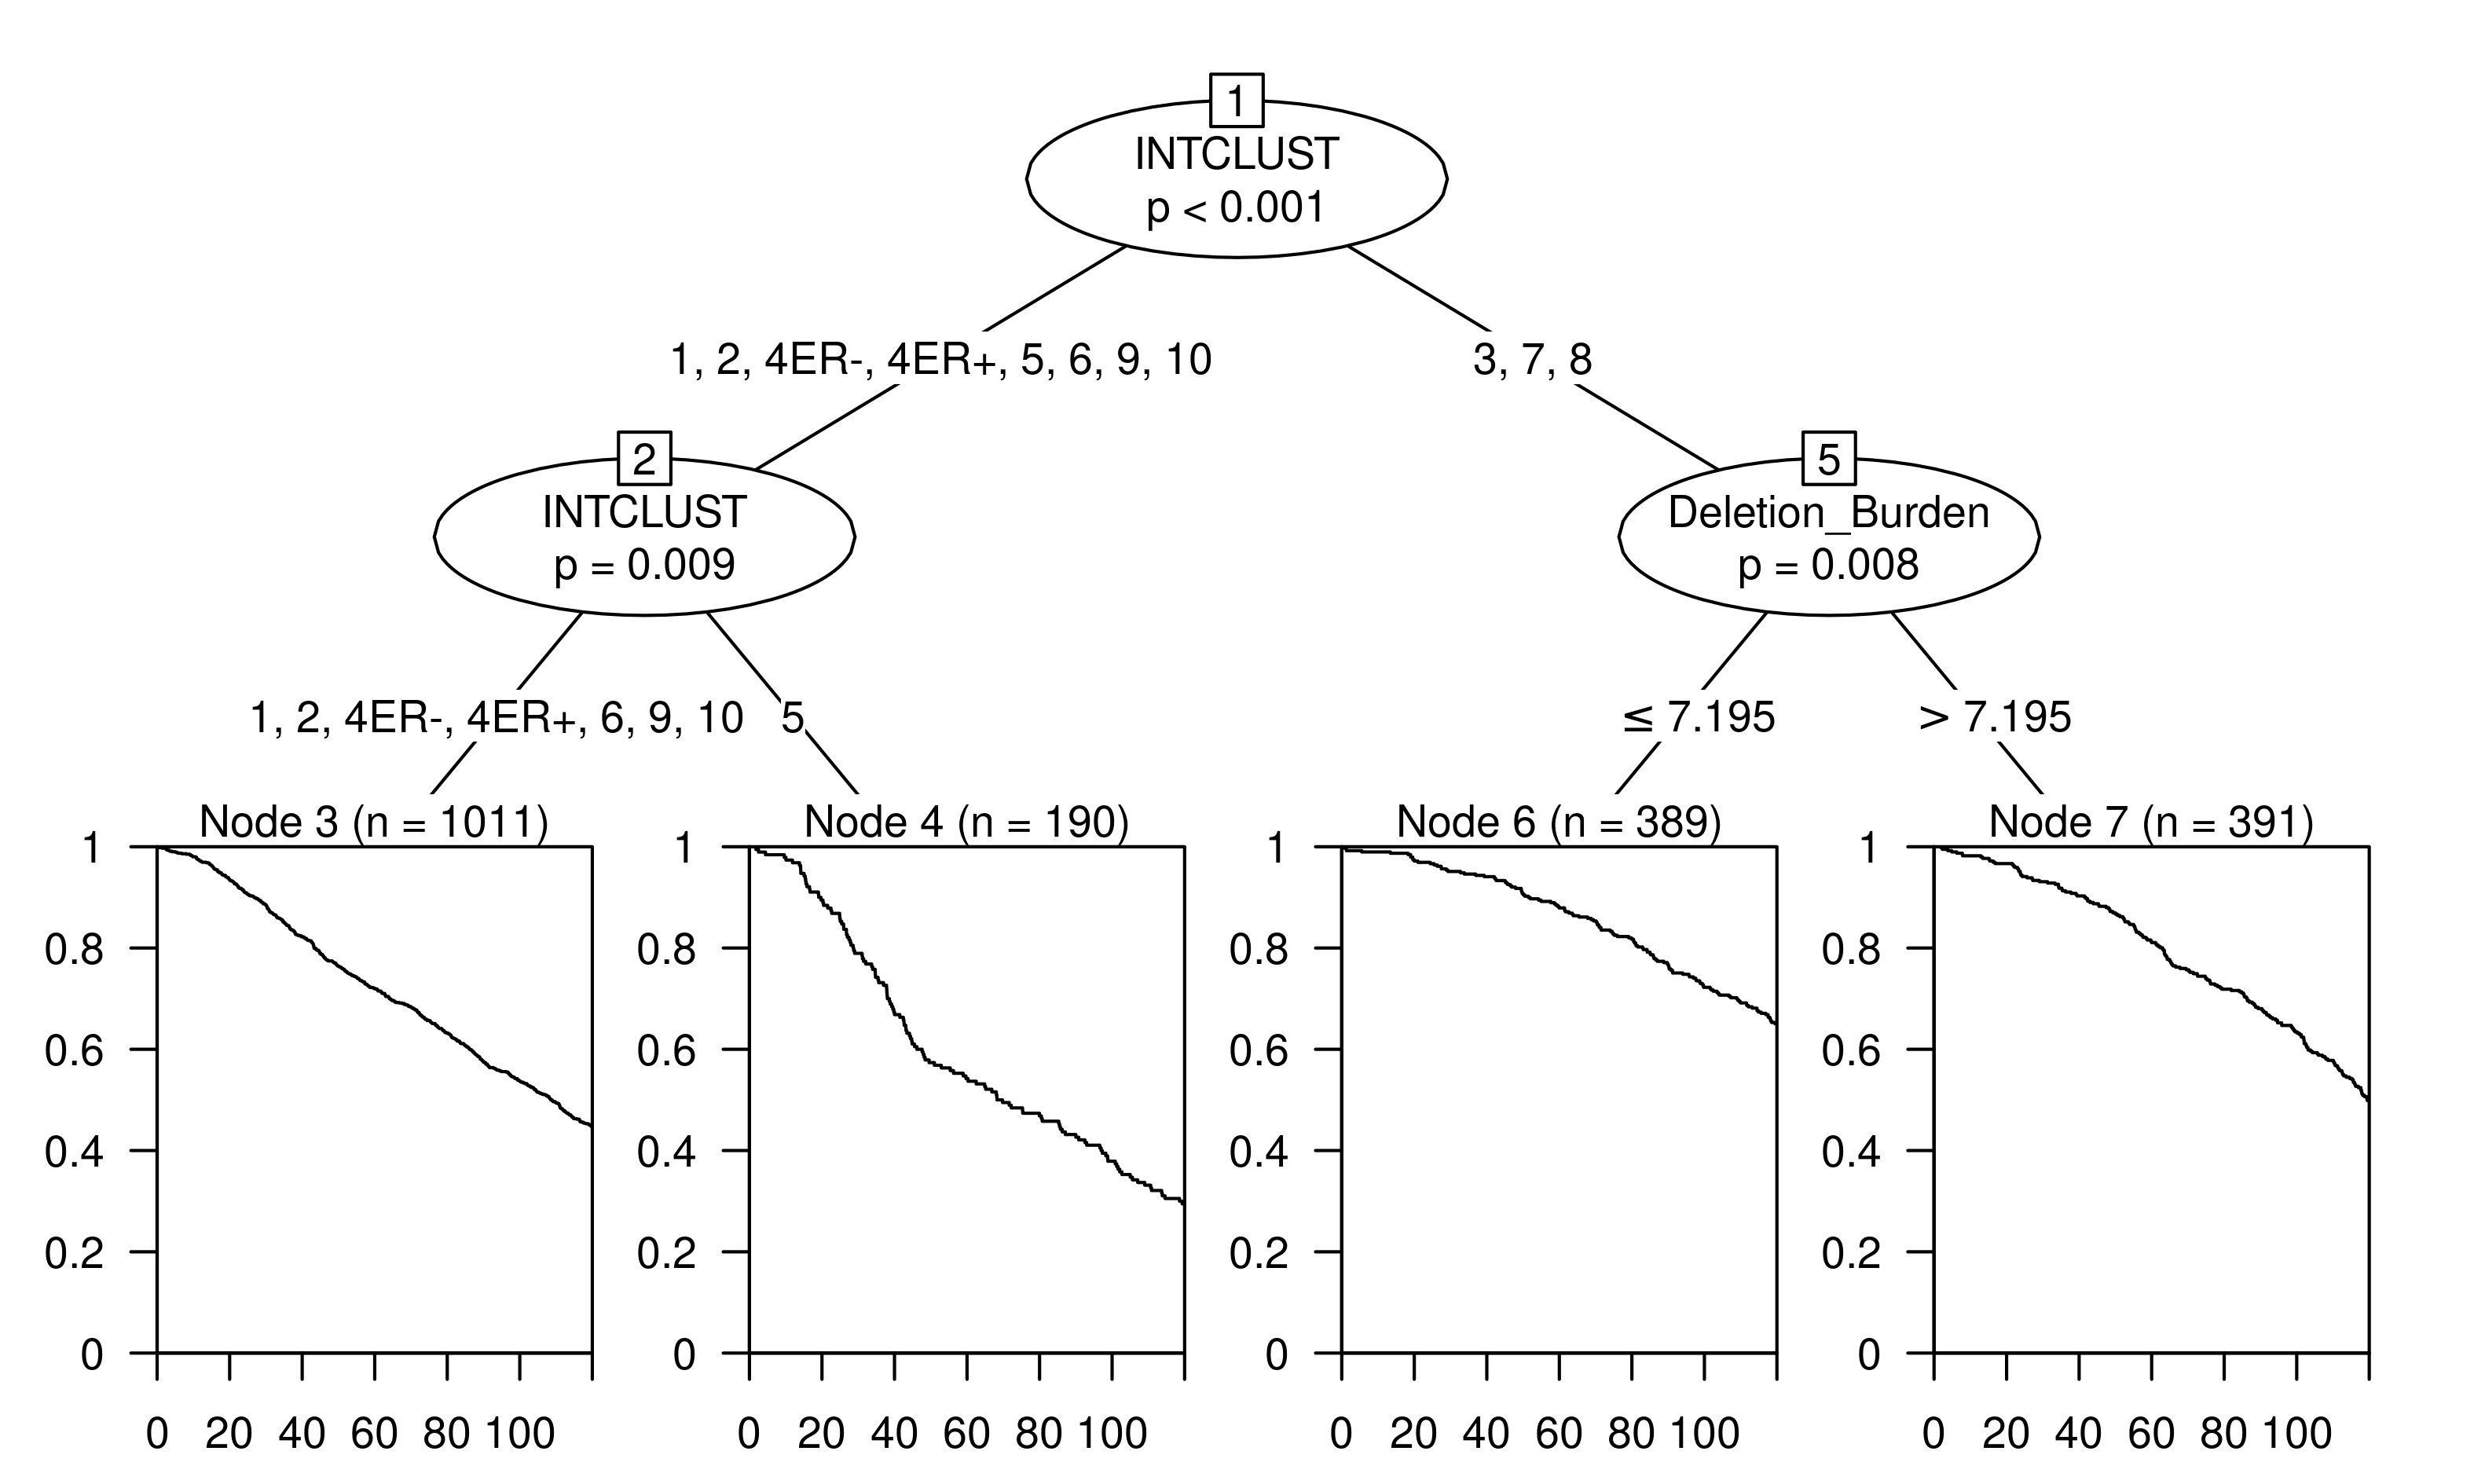
\includegraphics[width=1\textwidth]{../figures/Appendices/Appendix_B/Ctree_Survival_Burden_TenYearOS_INTCLUST.png}
\end{subfigure}

\vspace{0.5cm}

\caption[Recursive partitioning survival trees for ten-year overall survival using IntClust and the six CNA Burden metrics as candidate predictors.]{Recursive partitioning survival trees for ten-year overall survival using IntClust and the six CNA Burden metrics as candidate predictors. (A) Trees fitted using the rpart algorithm and (B) trees fitted using the ctree algorithm.}
\end{figure}

% OS using PAM50 Subtype, the six CNA Burden metrics and a number of clinical variables as candidate predictors
\begin{figure}[!htb]
\centering

\vspace{1cm}

\begin{subfigure}{\textwidth}
\subcaption{}
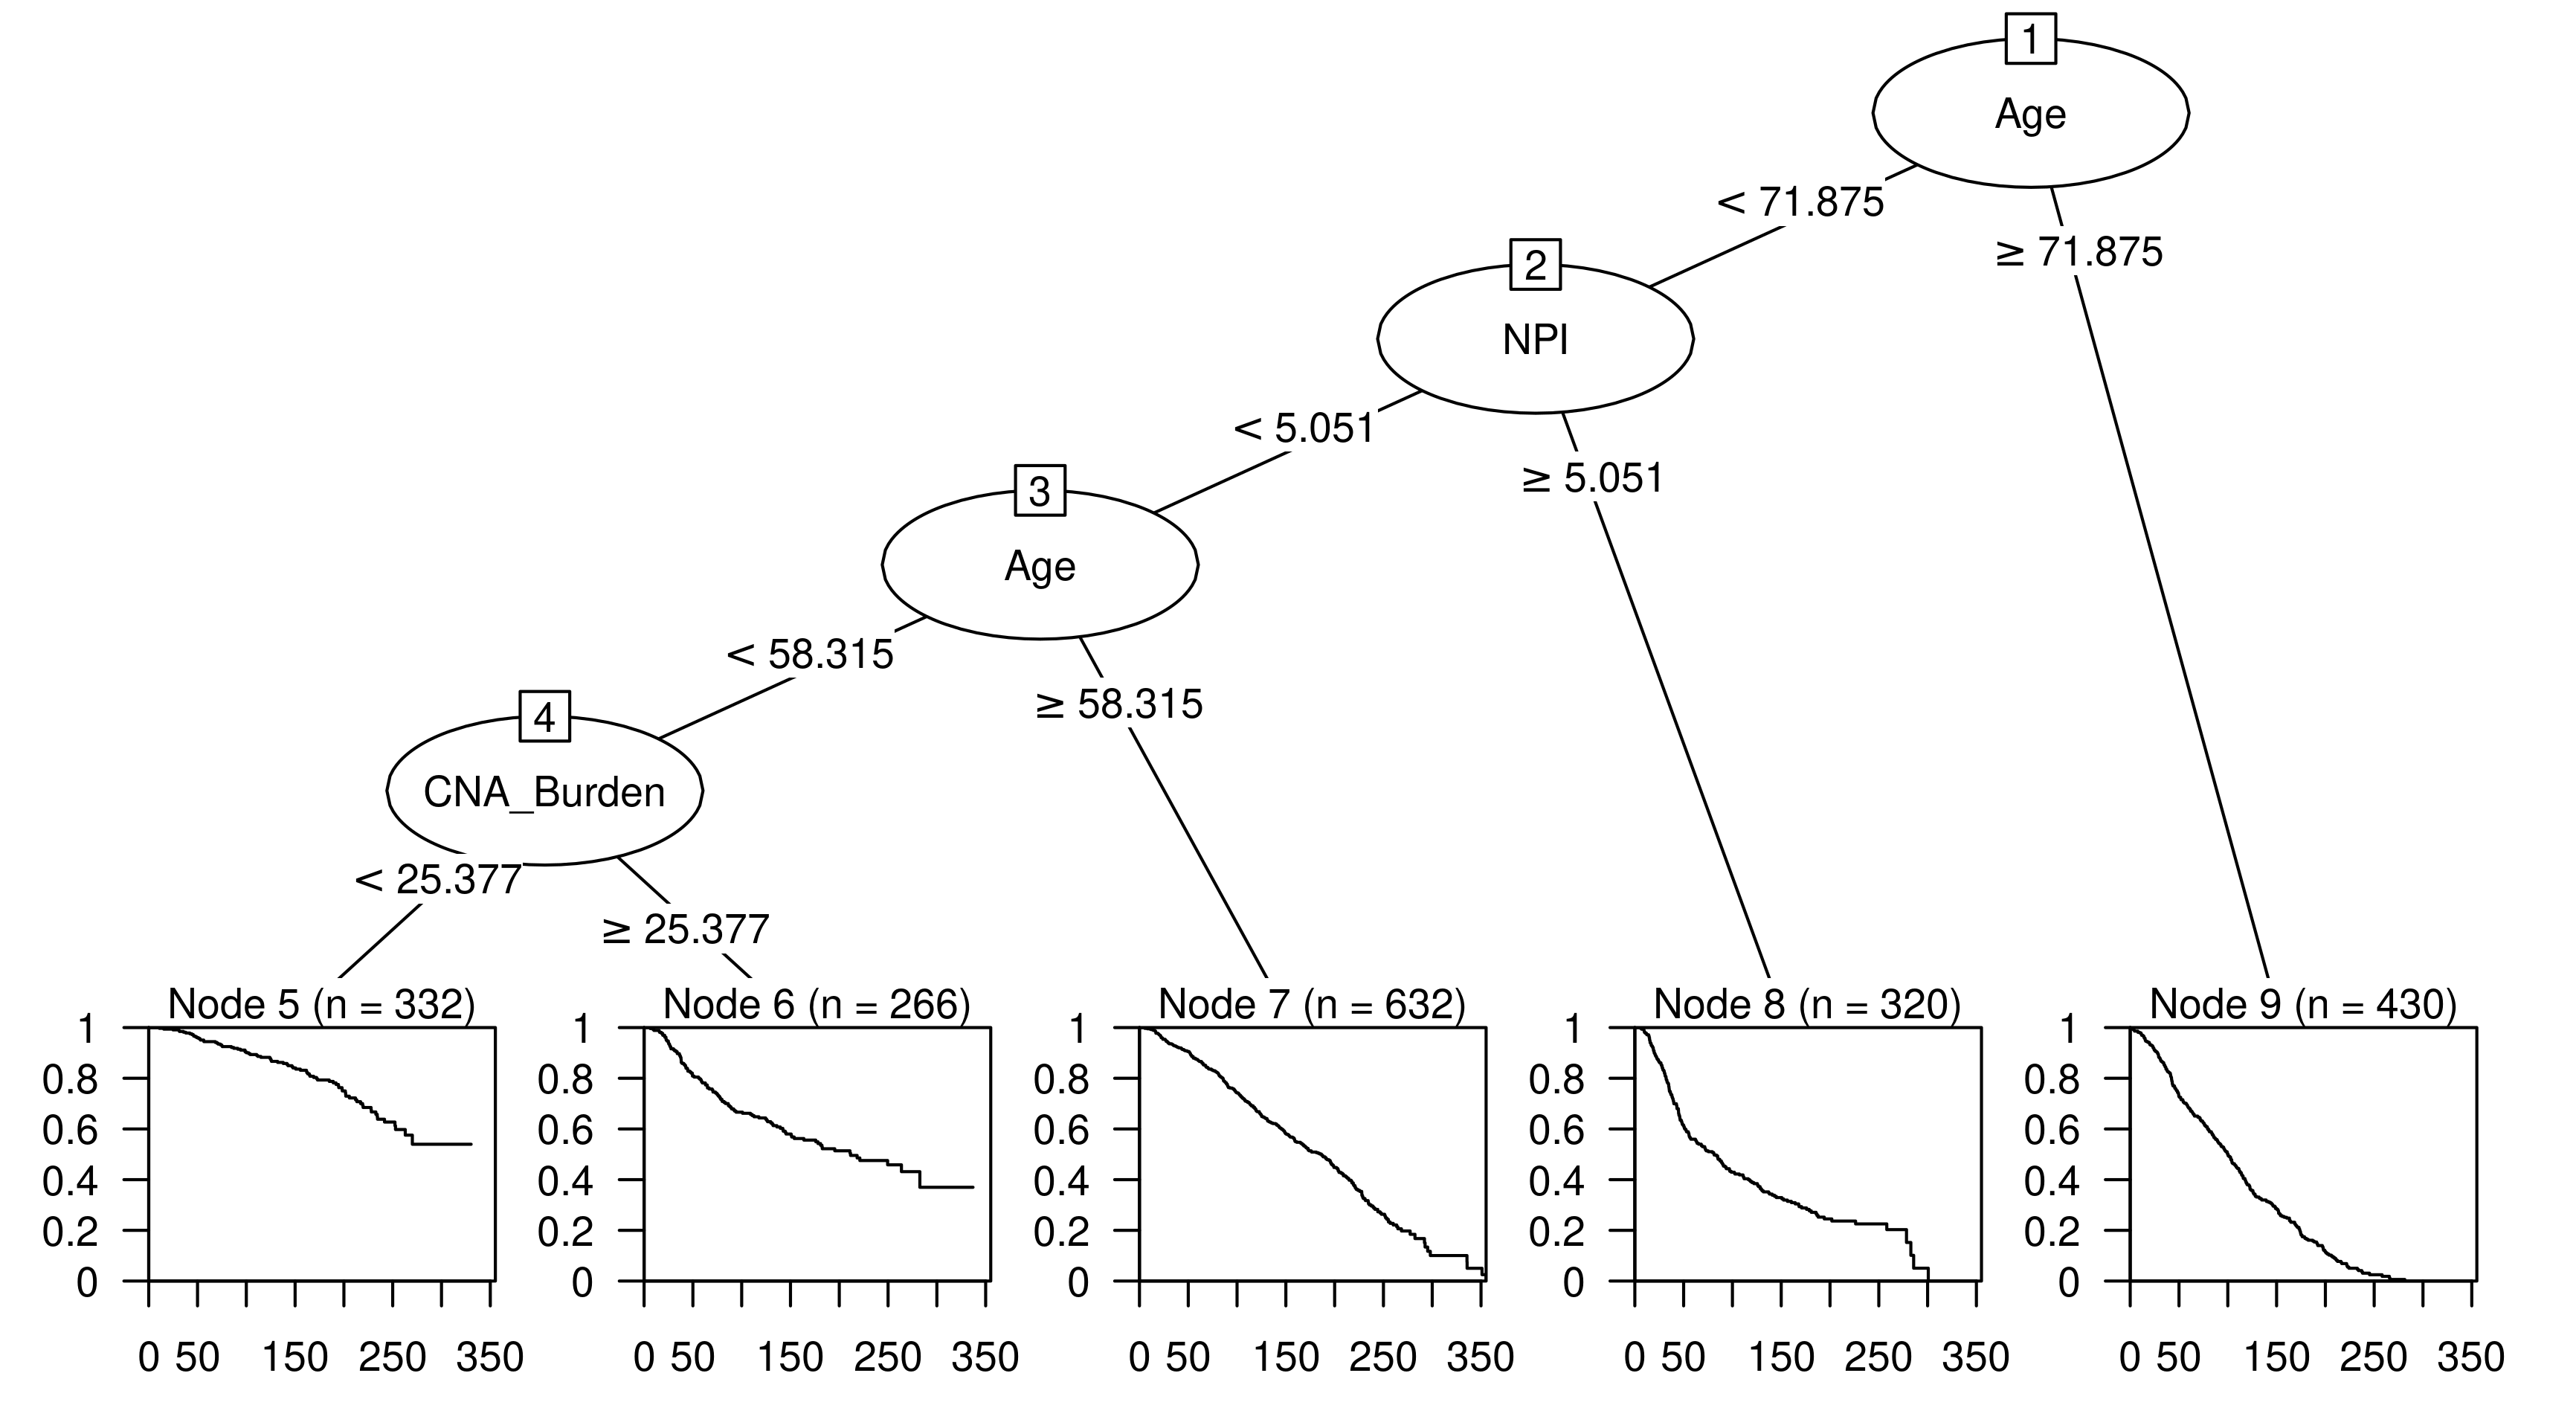
\includegraphics[width=1\textwidth]{../figures/Appendices/Appendix_B/Clin_PartyKit_Survival_Burden_OS_PAM50.png}
\end{subfigure}

\vspace{2cm}

\begin{subfigure}{\textwidth}
\subcaption{}
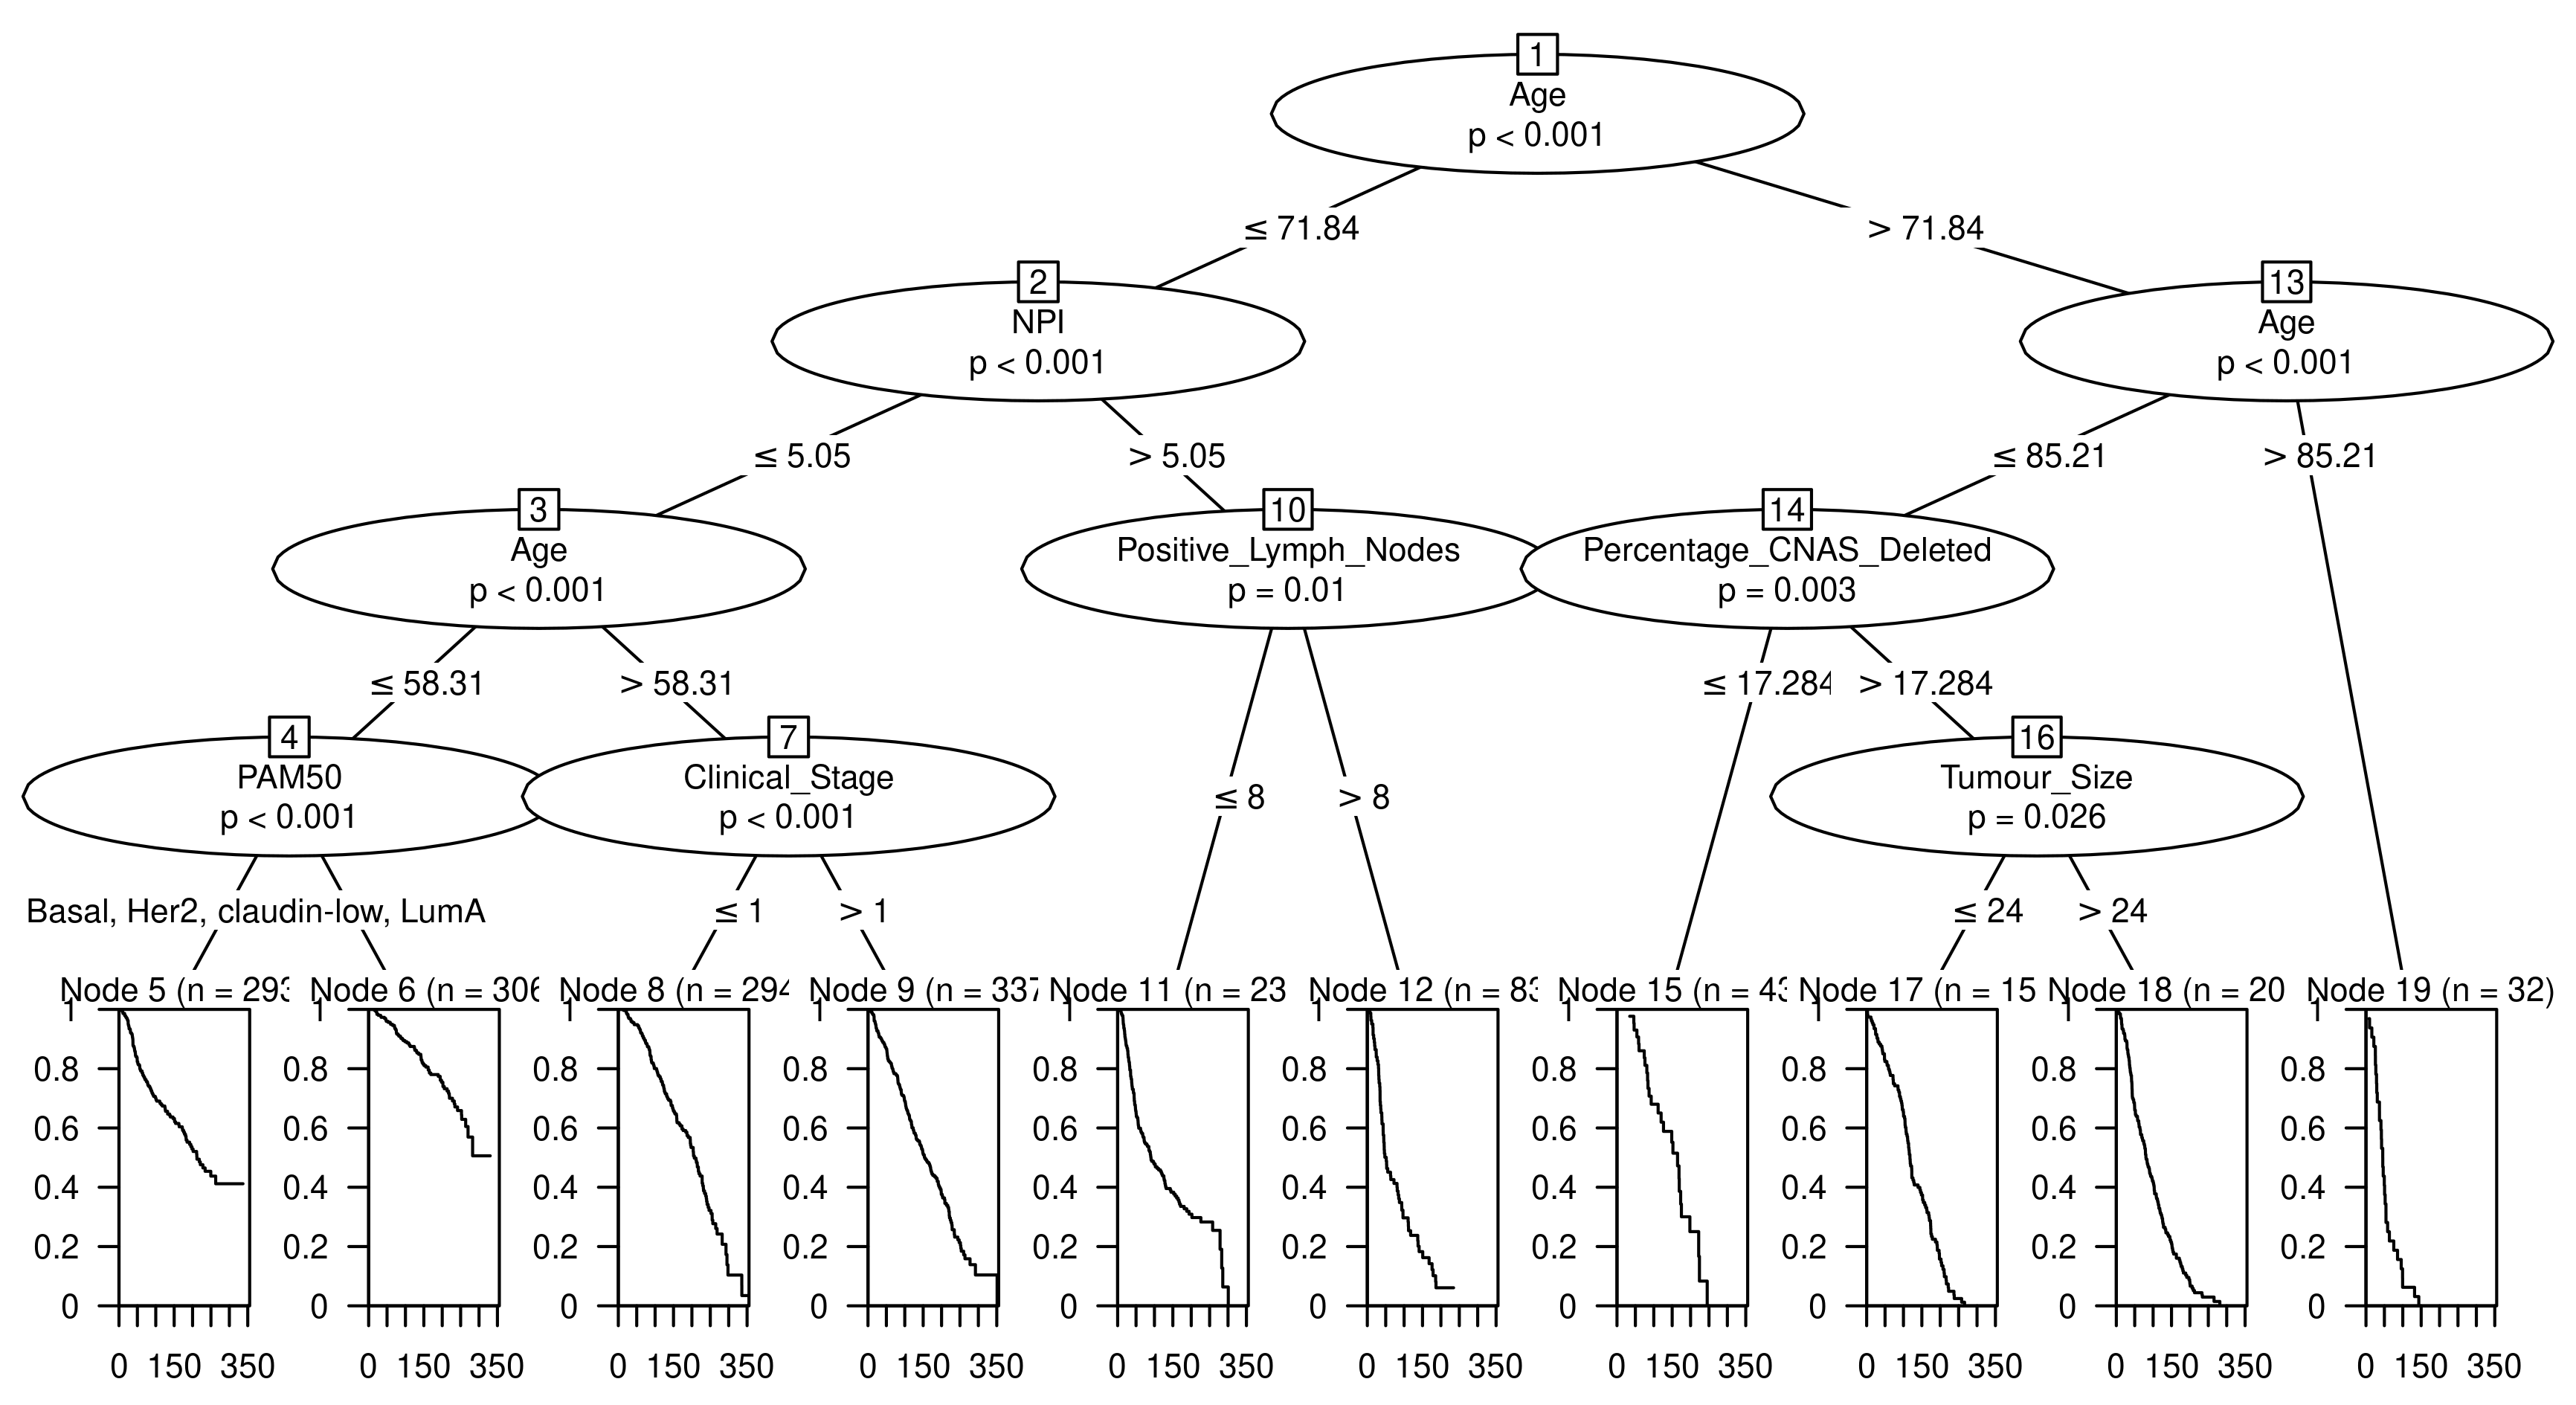
\includegraphics[width=1\textwidth]{../figures/Appendices/Appendix_B/Clin_Ctree_Survival_Burden_OS_PAM50.png}
\end{subfigure}

\vspace{1cm}

\caption[Recursive partitioning survival trees for overall survival using PAM50, the six CNA Burden metrics and a number of clinical variables as candidate predictors.]{Recursive partitioning survival trees for overall survival using PAM50, the six CNA Burden metrics and a number of clinical variables as candidate predictors. (A) Trees fitted using the rpart algorithm and (B) trees fitted using the ctree algorithm.}
\end{figure}

\begin{figure}[!htb]
\centering

\vspace{1cm}

\begin{subfigure}{\textwidth}
\subcaption{}
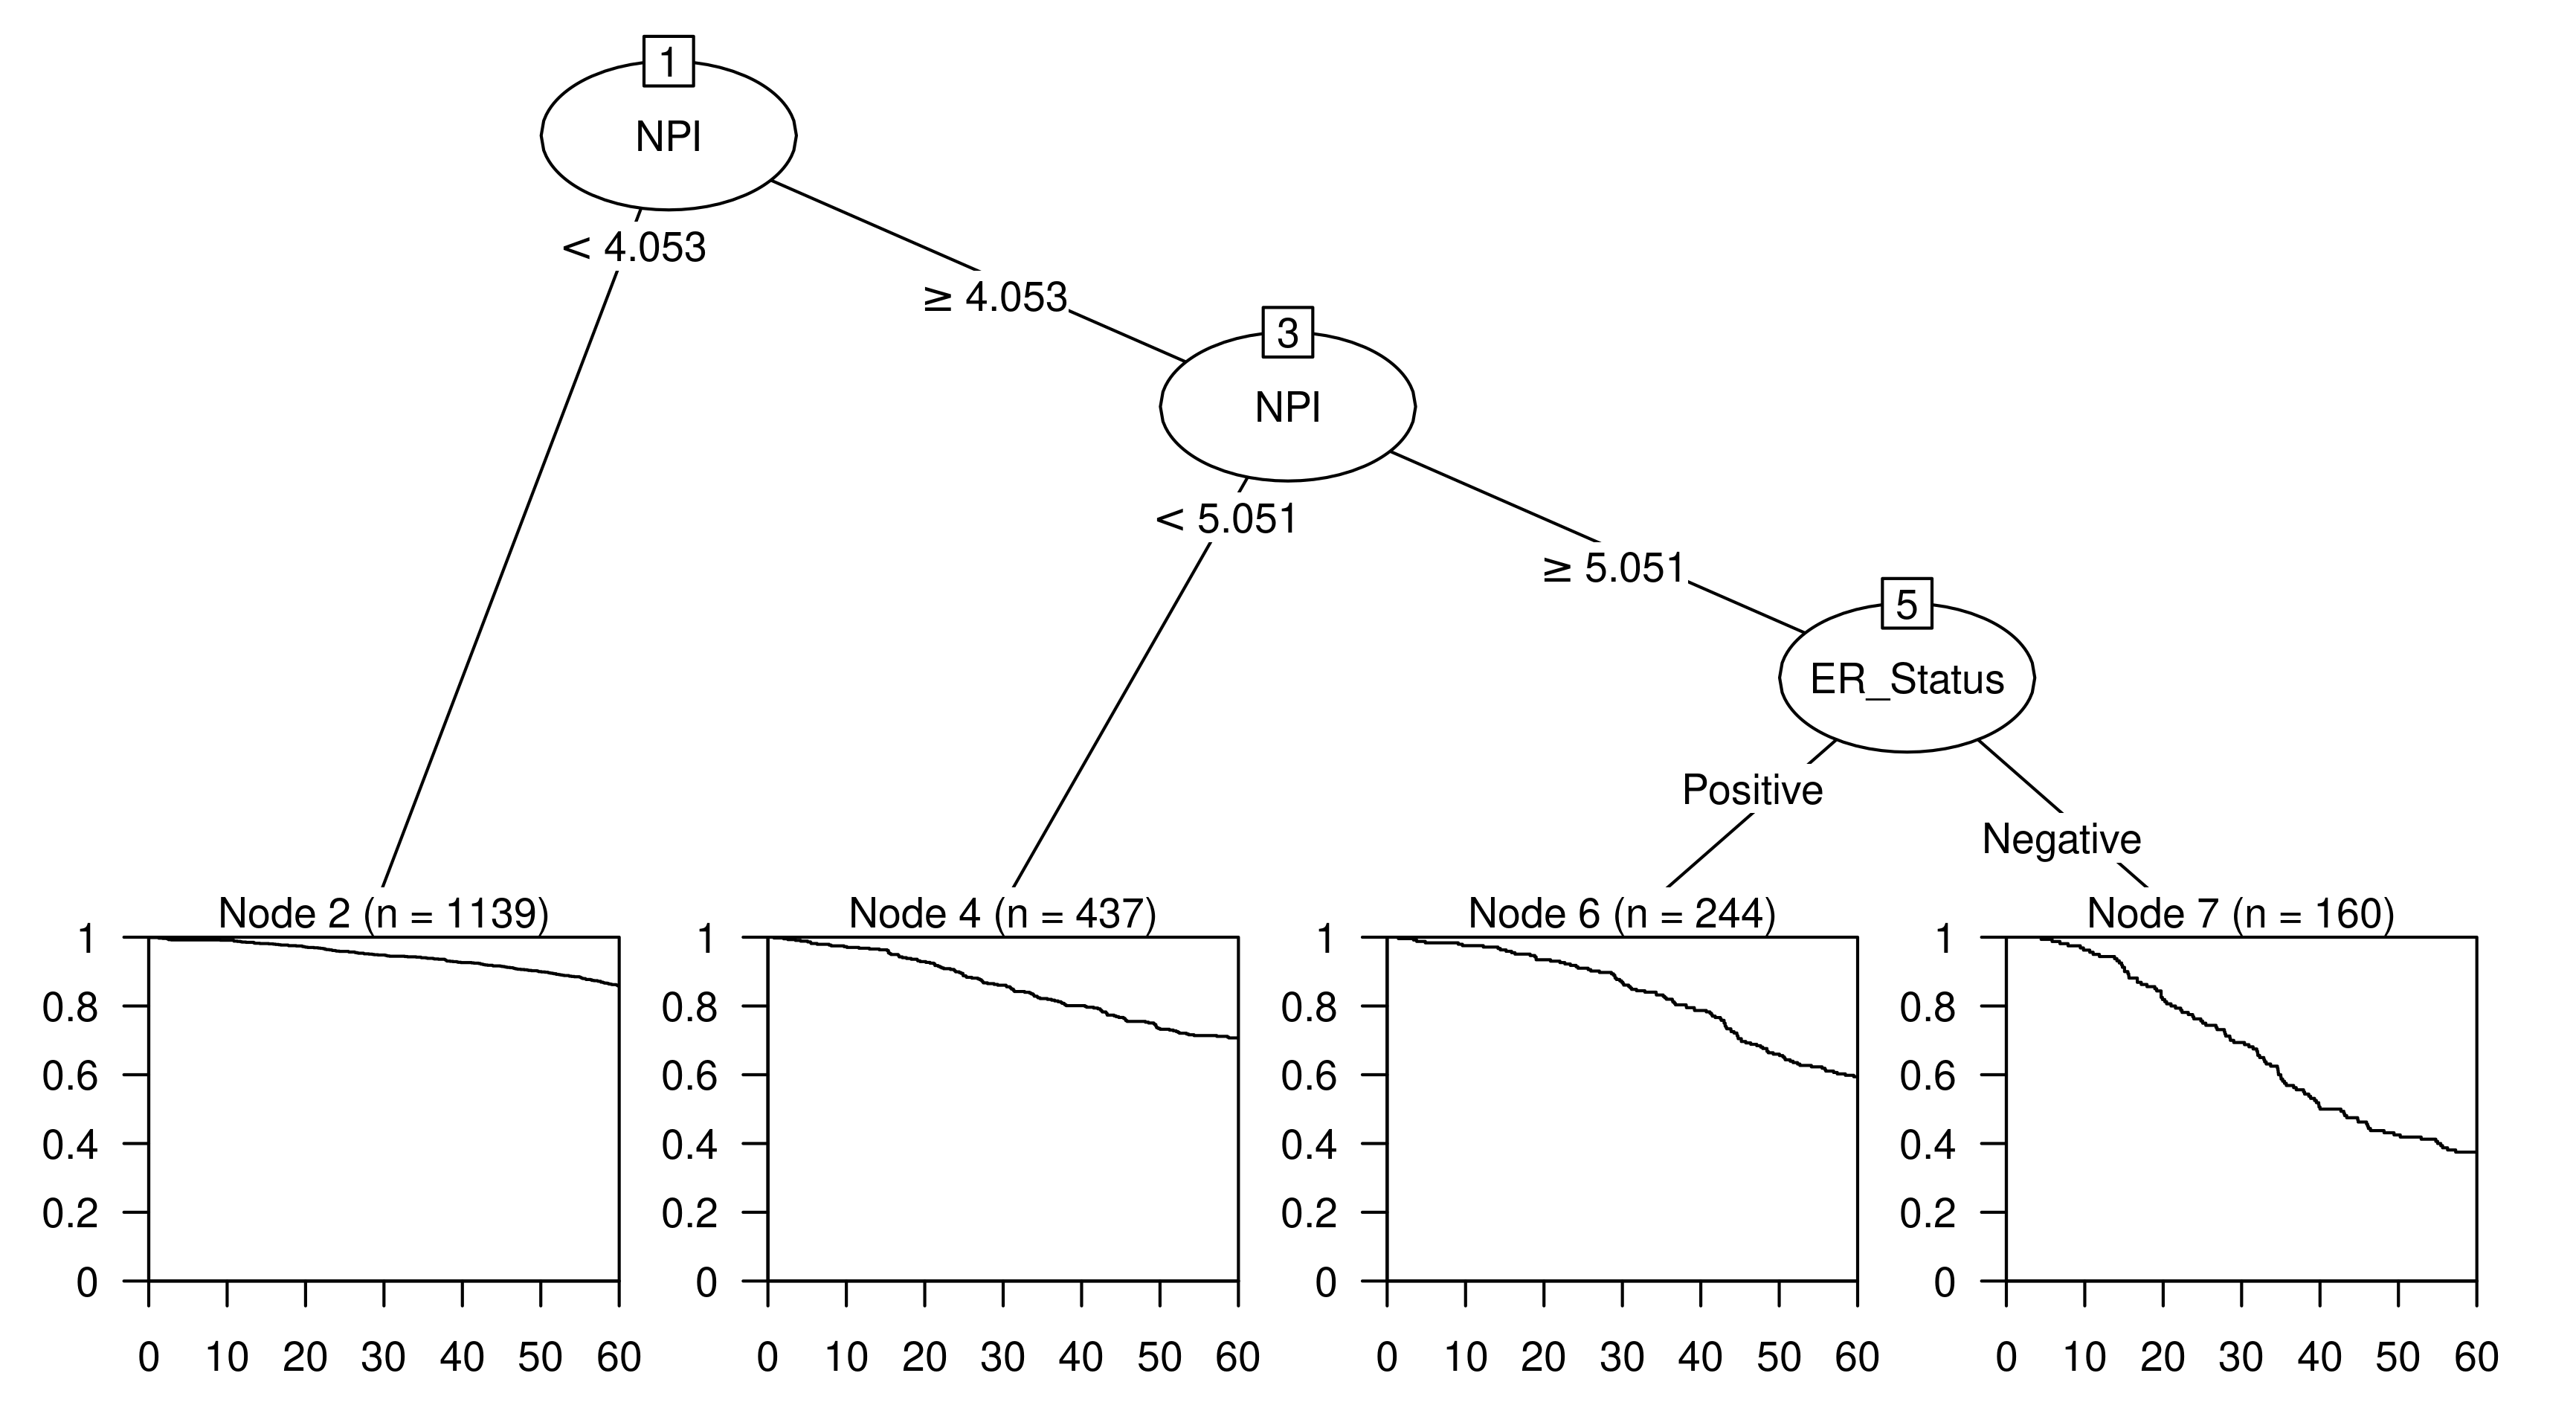
\includegraphics[width=1\textwidth]{../figures/Appendices/Appendix_B/Clin_PartyKit_Survival_Burden_FiveYearOS_PAM50.png}
\end{subfigure}

\vspace{2cm}

\begin{subfigure}{\textwidth}
\subcaption{}
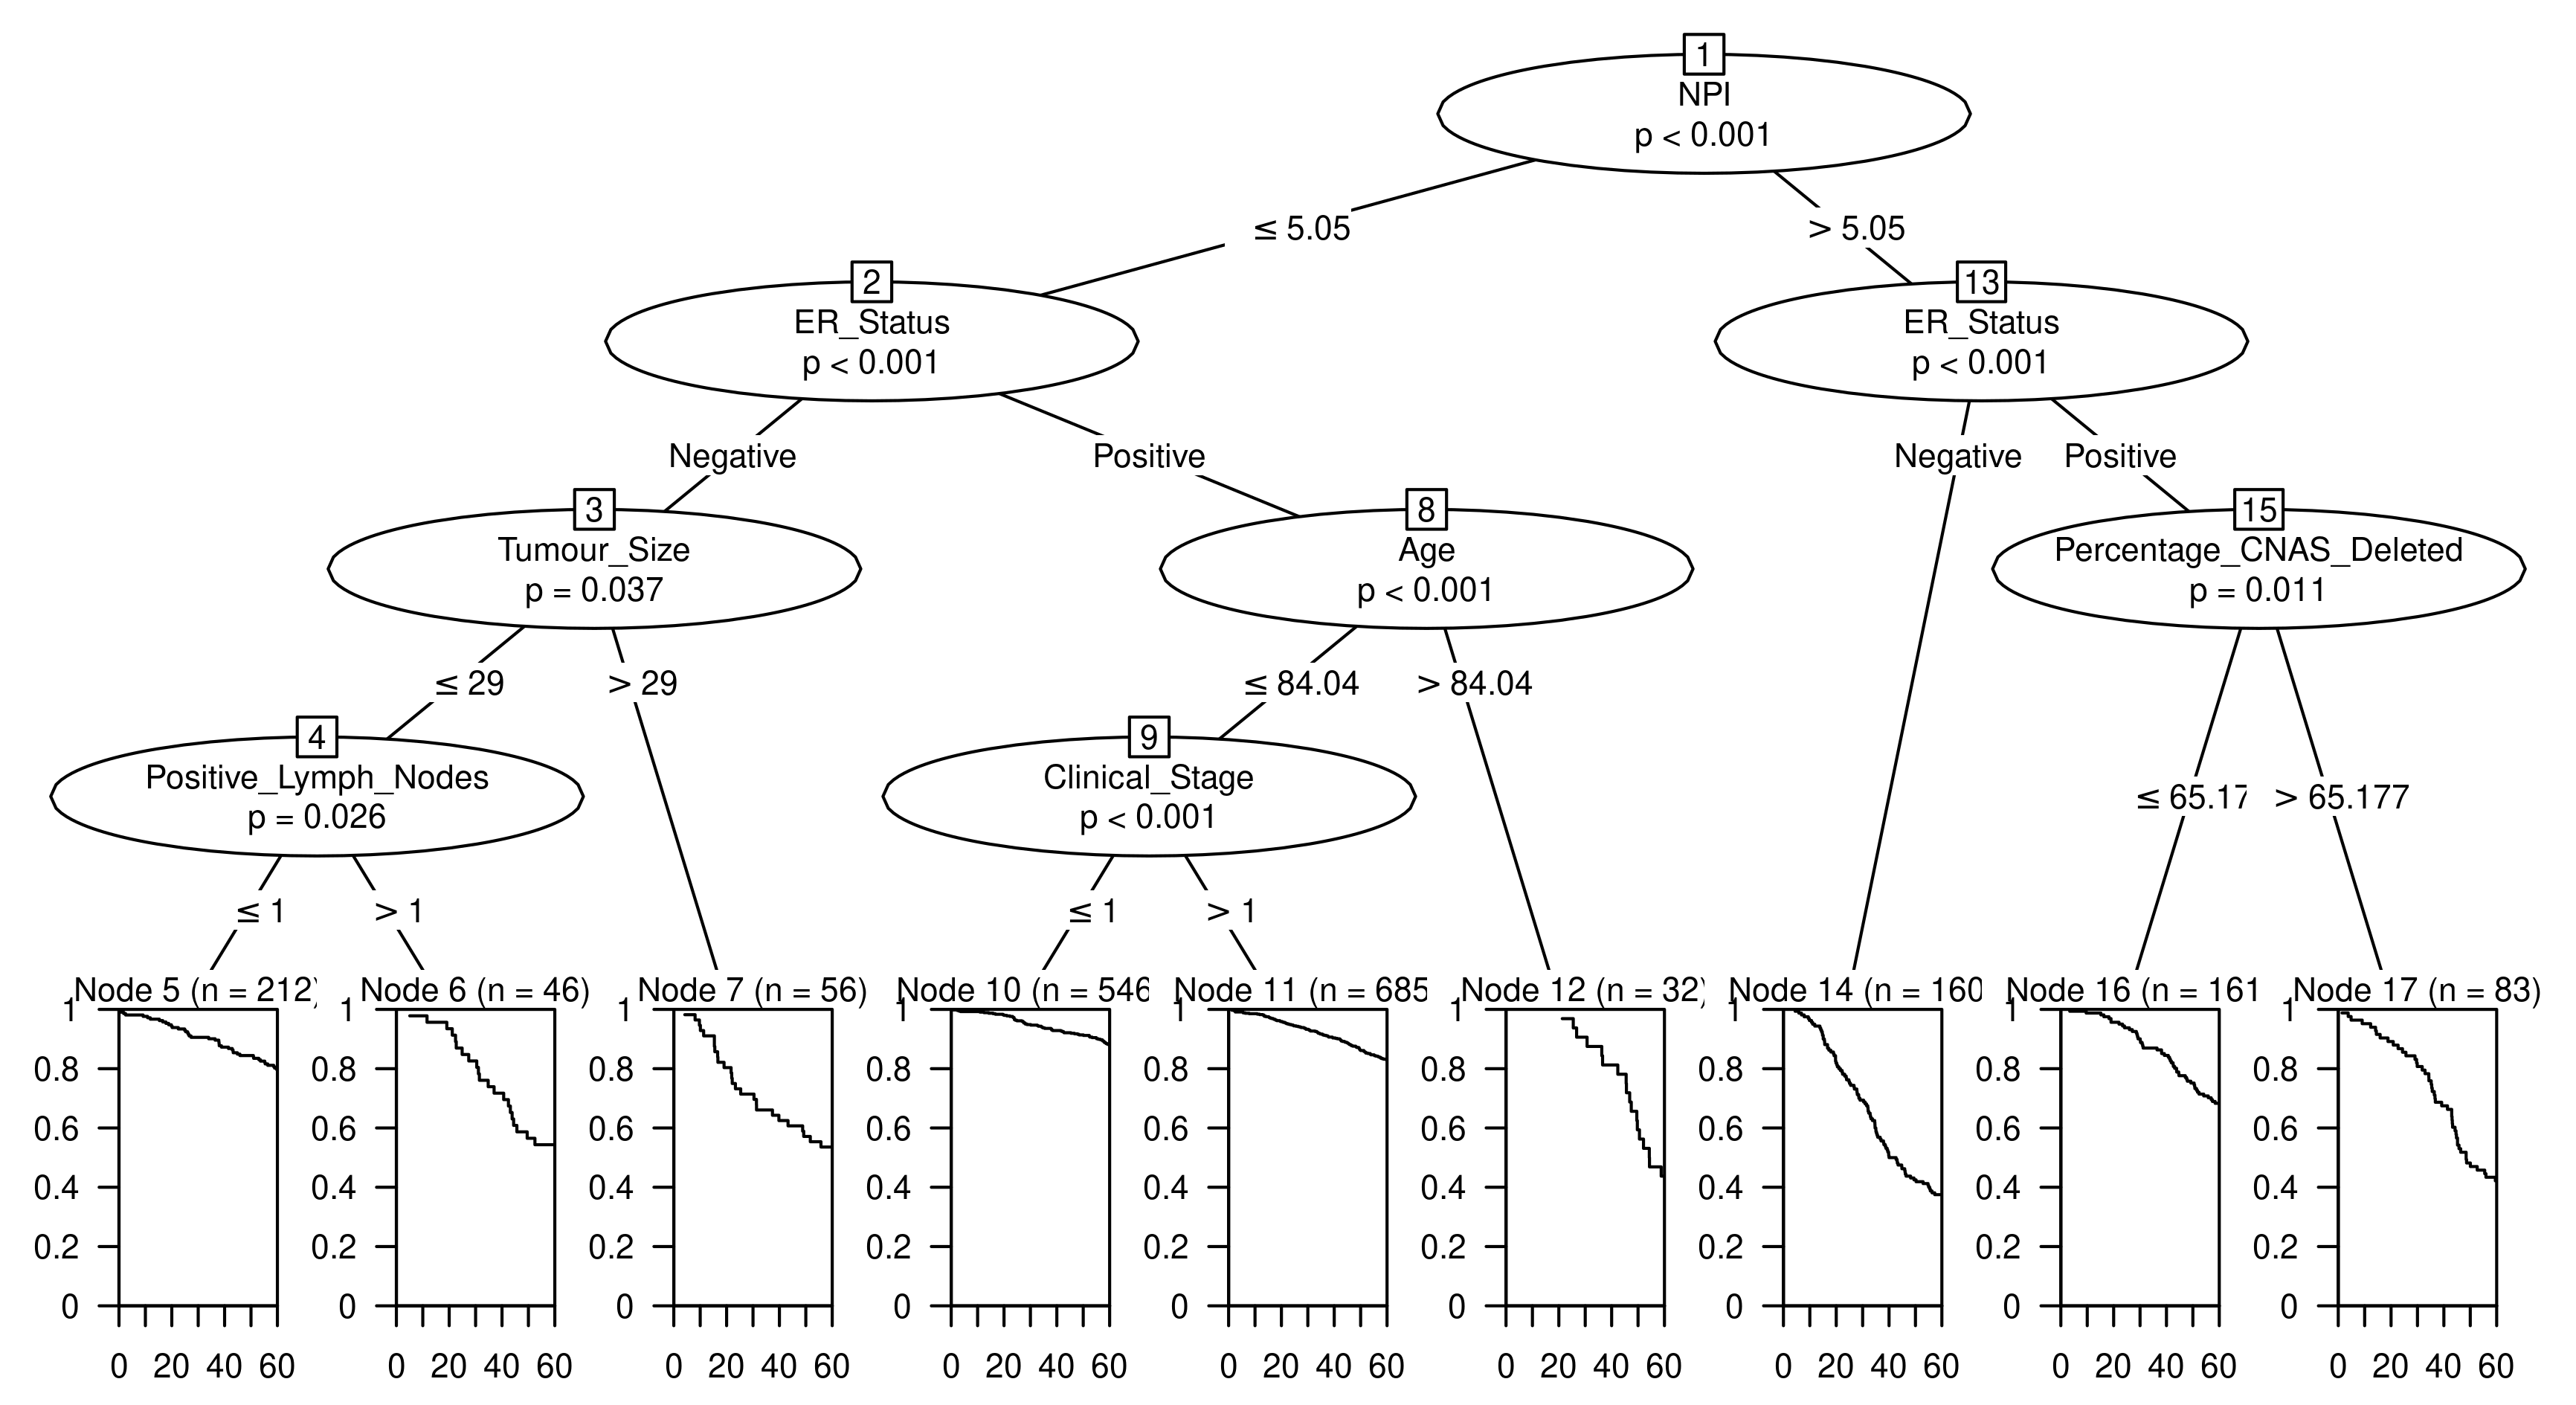
\includegraphics[width=1\textwidth]{../figures/Appendices/Appendix_B/Clin_Ctree_Survival_Burden_FiveYearOS_PAM50.png}
\end{subfigure}

\vspace{1cm}

\caption[Recursive partitioning survival trees for five-year overall survival using PAM50, the six CNA Burden metrics and a number of clinical variables as candidate predictors.]{Recursive partitioning survival trees for five-year overall survival using PAM50, the six CNA Burden metrics and a number of clinical variables as candidate predictors. (A) Trees fitted using the rpart algorithm and (B) trees fitted using the ctree algorithm.}
\end{figure}

\begin{figure}[!htb]
\centering

\vspace{1cm}

\begin{subfigure}{\textwidth}
\subcaption{}
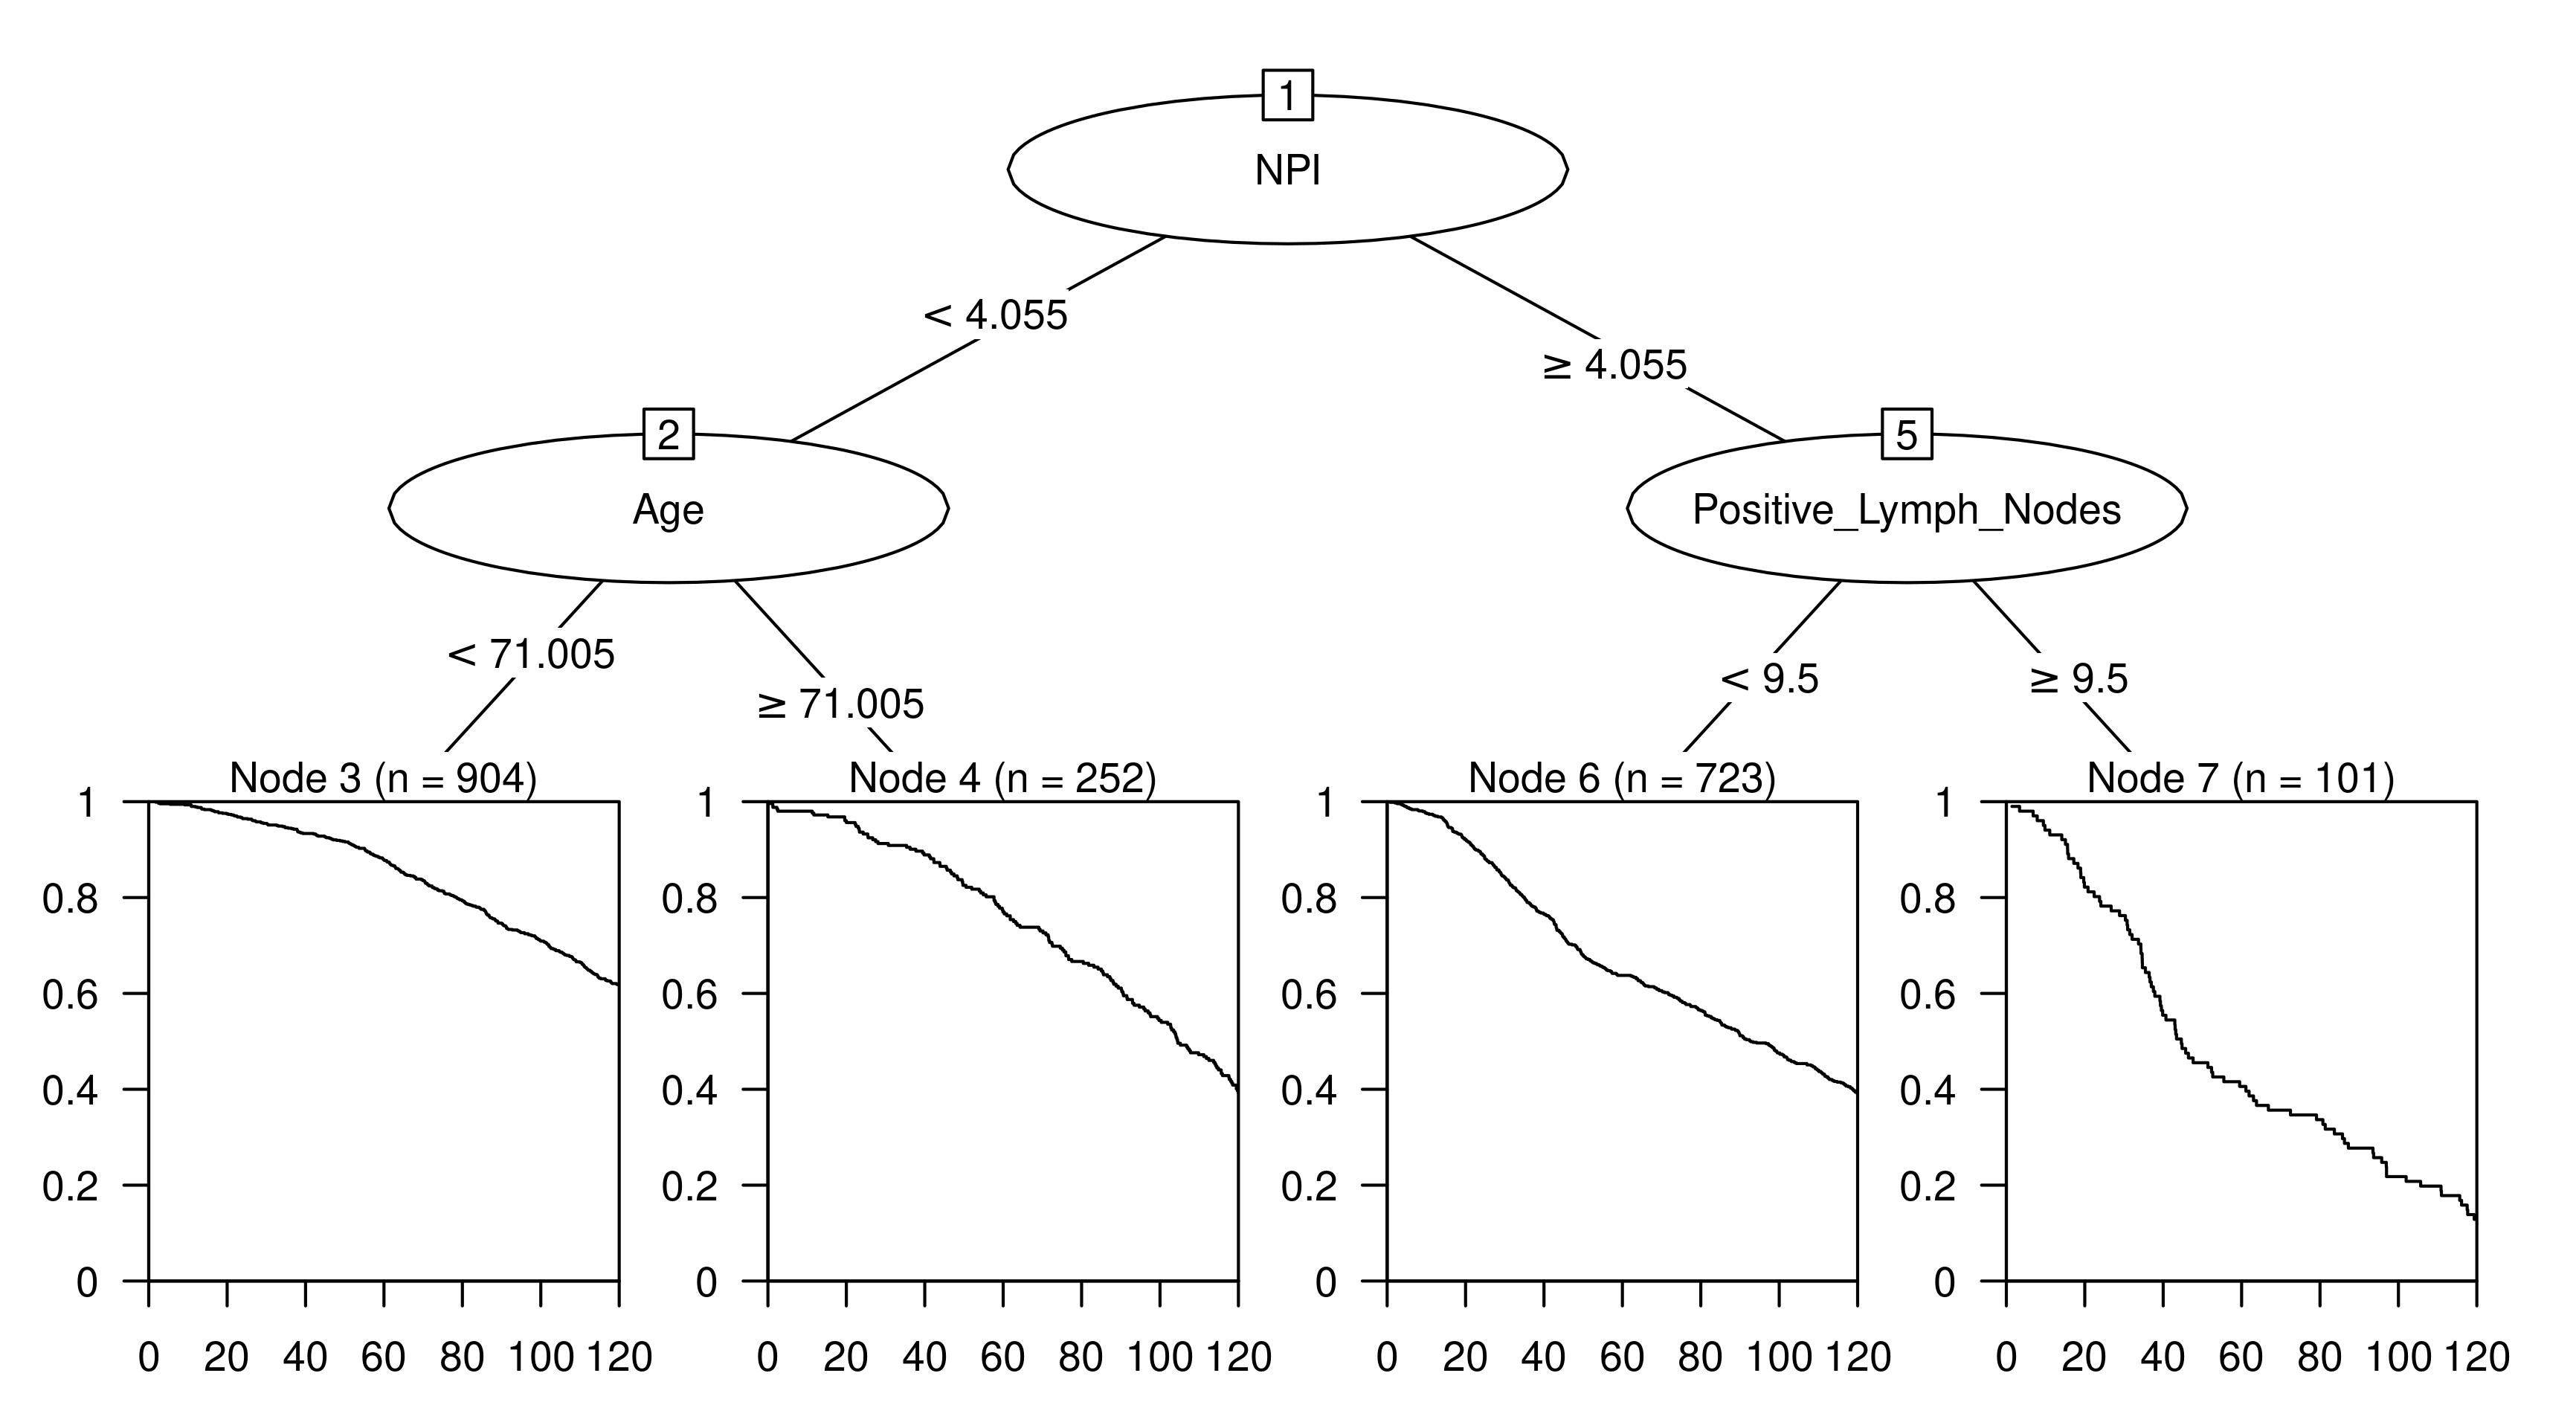
\includegraphics[width=1\textwidth]{../figures/Appendices/Appendix_B/Clin_PartyKit_Survival_Burden_TenYearOS_PAM50.png}
\end{subfigure}

\vspace{2cm}

\begin{subfigure}{\textwidth}
\subcaption{}
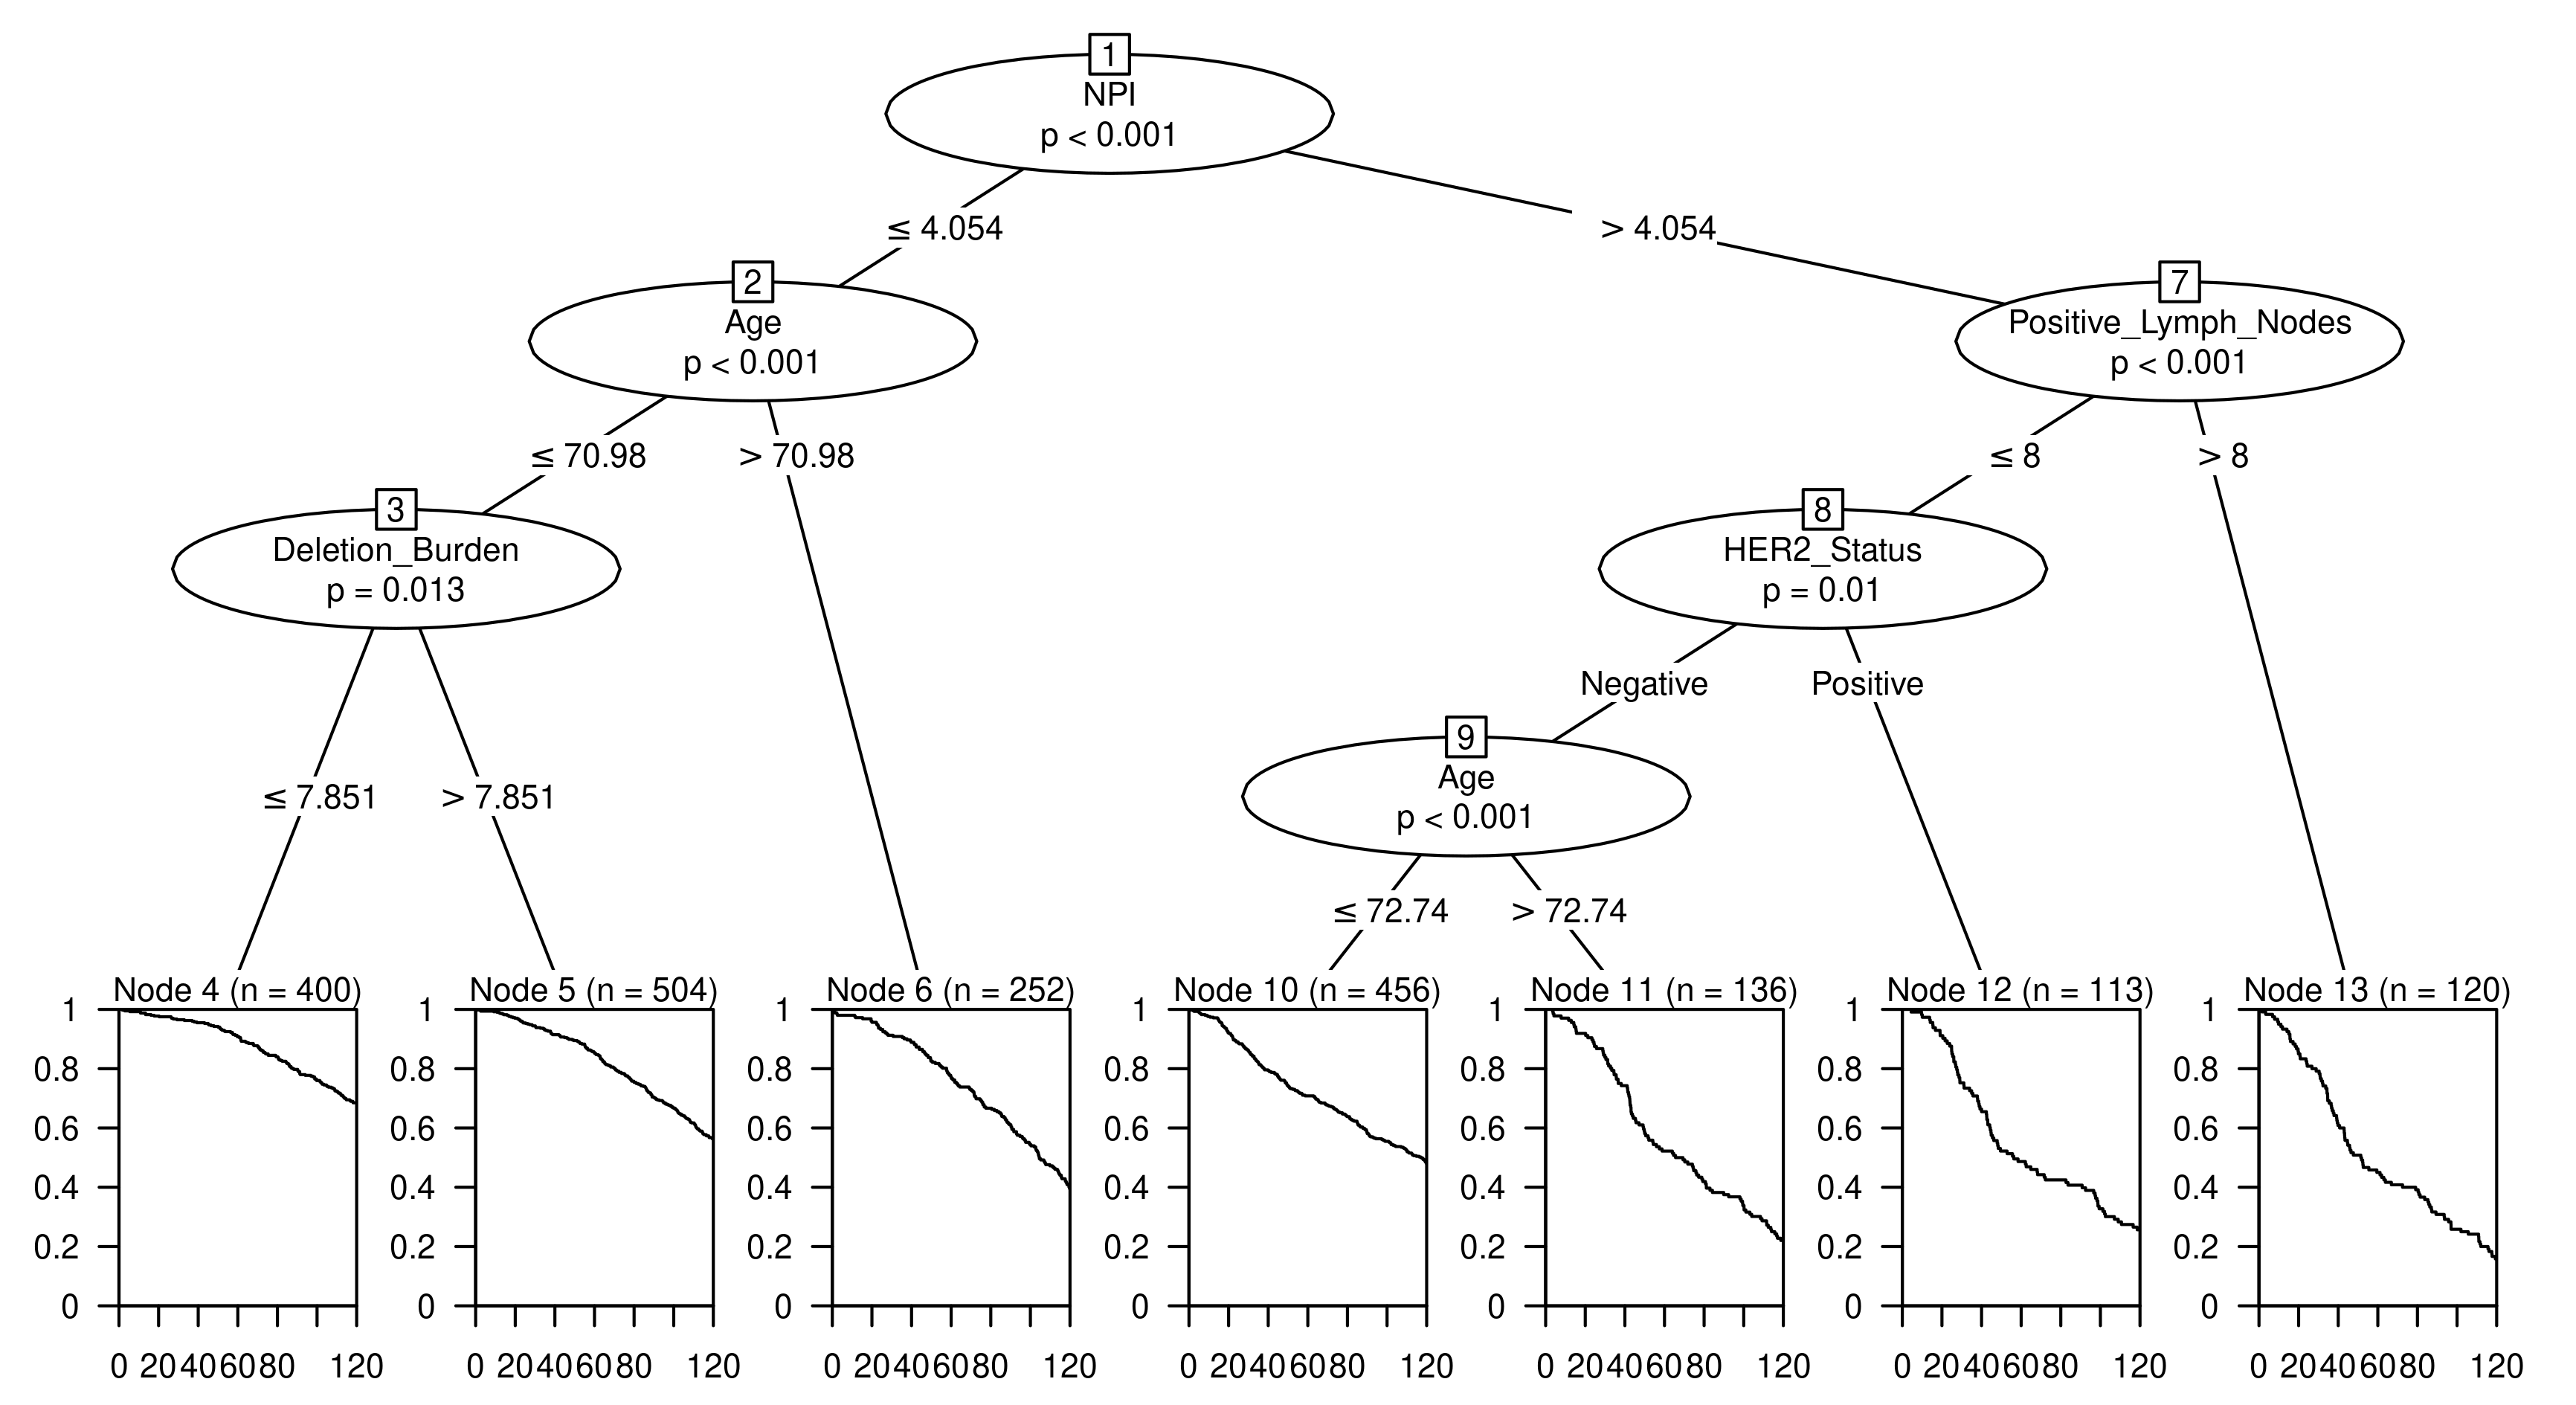
\includegraphics[width=1\textwidth]{../figures/Appendices/Appendix_B/Clin_Ctree_Survival_Burden_TenYearOS_PAM50.png}
\end{subfigure}

\vspace{1cm}

\caption[Recursive partitioning survival trees for ten-year overall survival using PAM50, the six CNA Burden metrics and a number of clinical variables as candidate predictors.]{Recursive partitioning survival trees for ten-year overall survival using PAM50, the six CNA Burden metrics and a number of clinical variables as candidate predictors. (A) Trees fitted using the rpart algorithm and (B) trees fitted using the ctree algorithm.}
\end{figure}

\begin{figure}[!htb]
\centering

\vspace{1cm}

\begin{subfigure}{\textwidth}
\subcaption{}
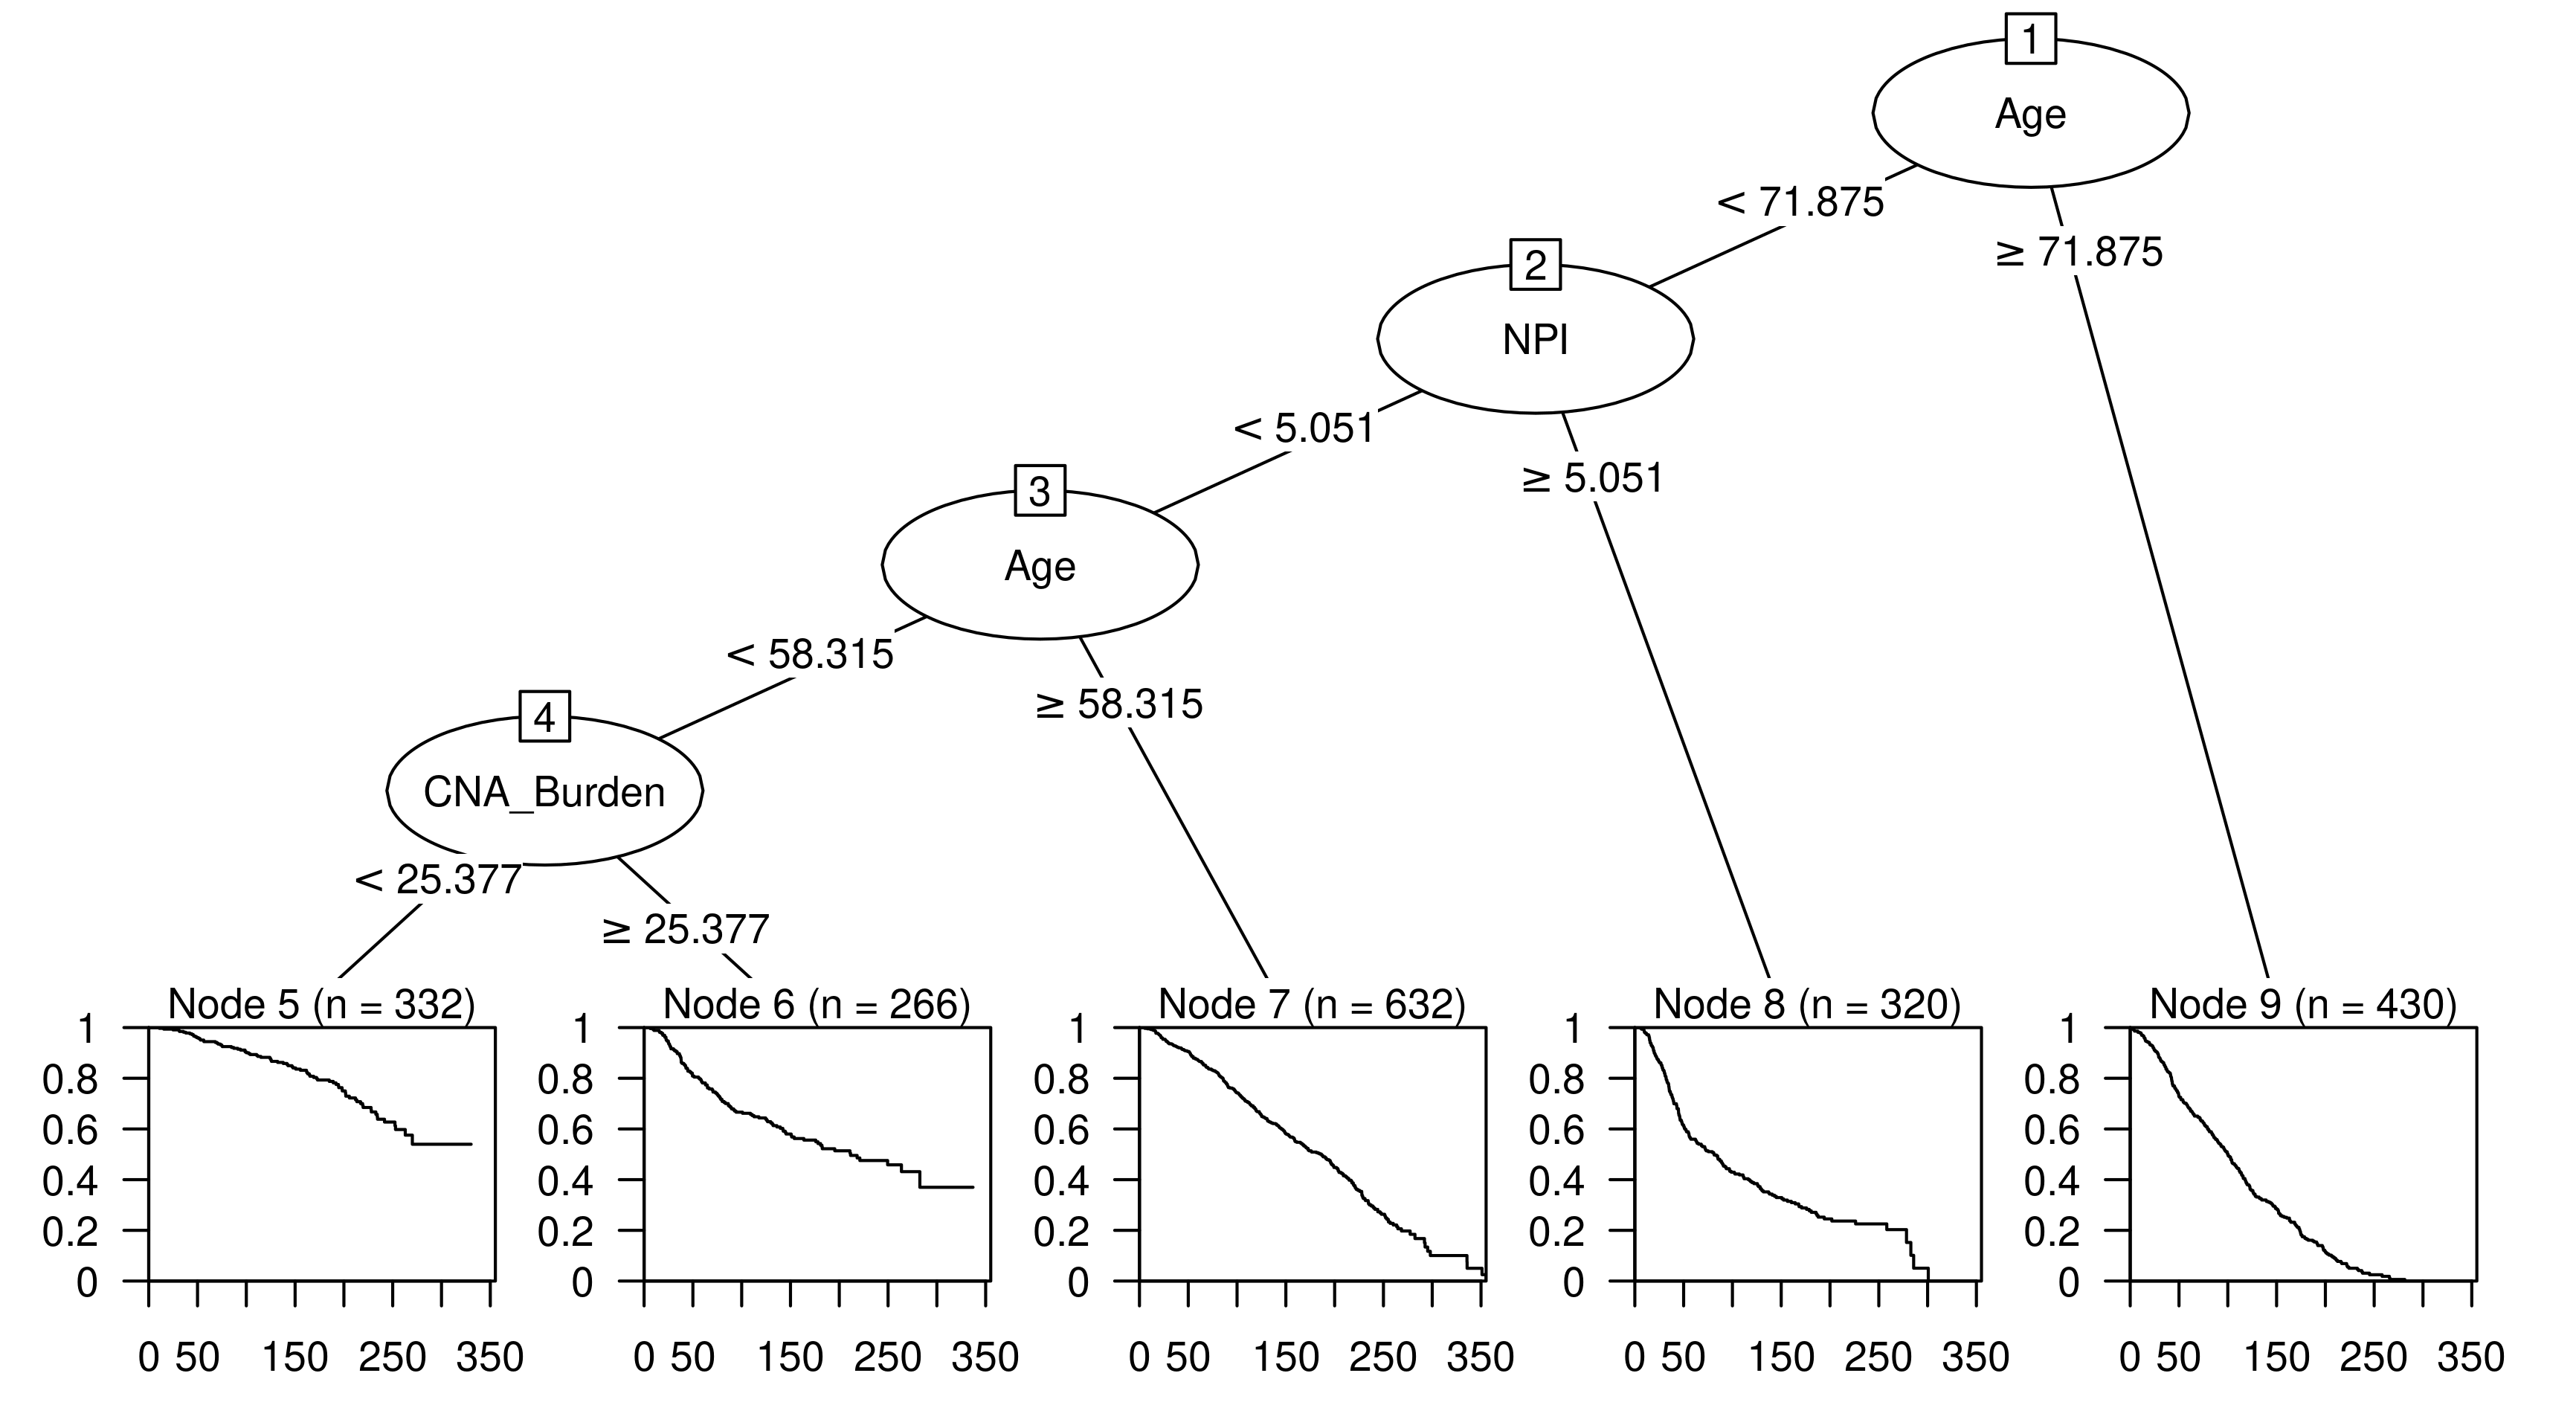
\includegraphics[width=1\textwidth]{../figures/Appendices/Appendix_B/Clin_PartyKit_Survival_Burden_OS_INTCLUST.png}
\end{subfigure}

\vspace{2cm}

\begin{subfigure}{\textwidth}
\subcaption{}
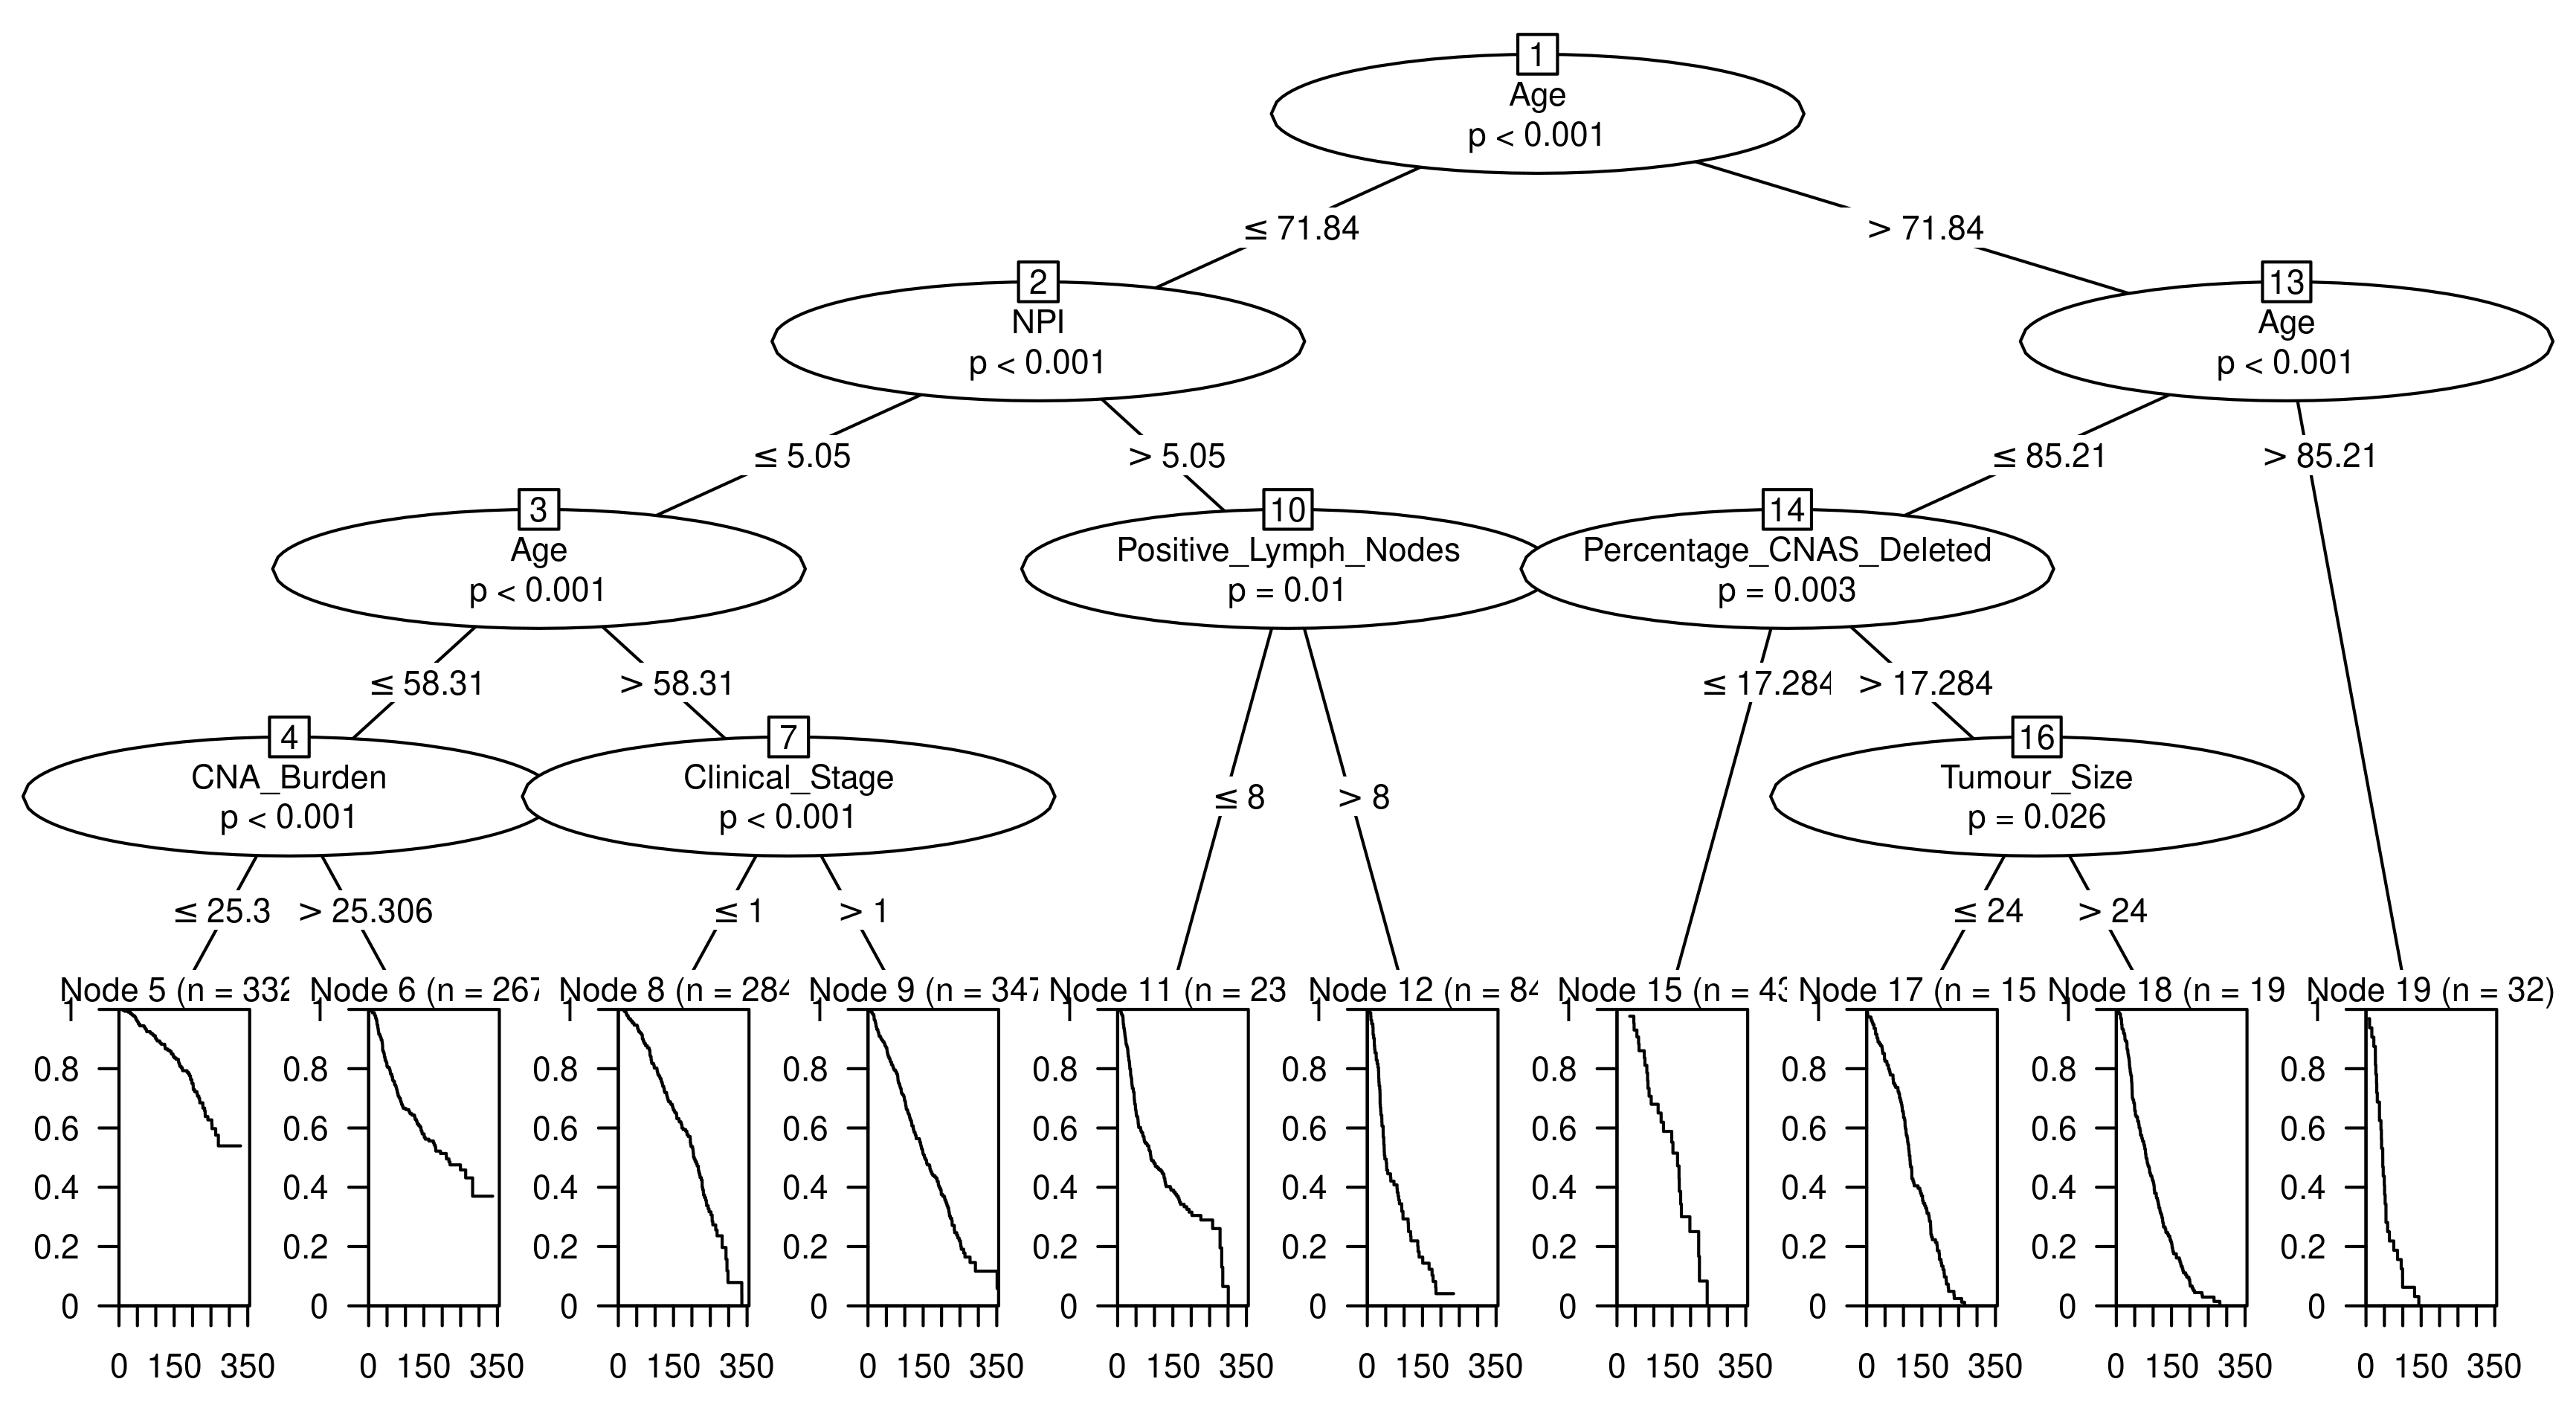
\includegraphics[width=1\textwidth]{../figures/Appendices/Appendix_B/Clin_Ctree_Survival_Burden_OS_INTCLUST.png}
\end{subfigure}

\vspace{1cm}

\caption[Recursive partitioning survival trees for overall survival using INTCLUST, the six CNA Burden metrics and a number of clinical variables as candidate predictors.]{Recursive partitioning survival trees for overall survival using INTCLUST, the six CNA Burden metrics and a number of clinical variables as candidate predictors. (A) Trees fitted using the rpart algorithm and (B) trees fitted using the ctree algorithm.}
\end{figure}

\begin{figure}[!htb]
\centering

\vspace{1cm}

\begin{subfigure}{\textwidth}
\subcaption{}
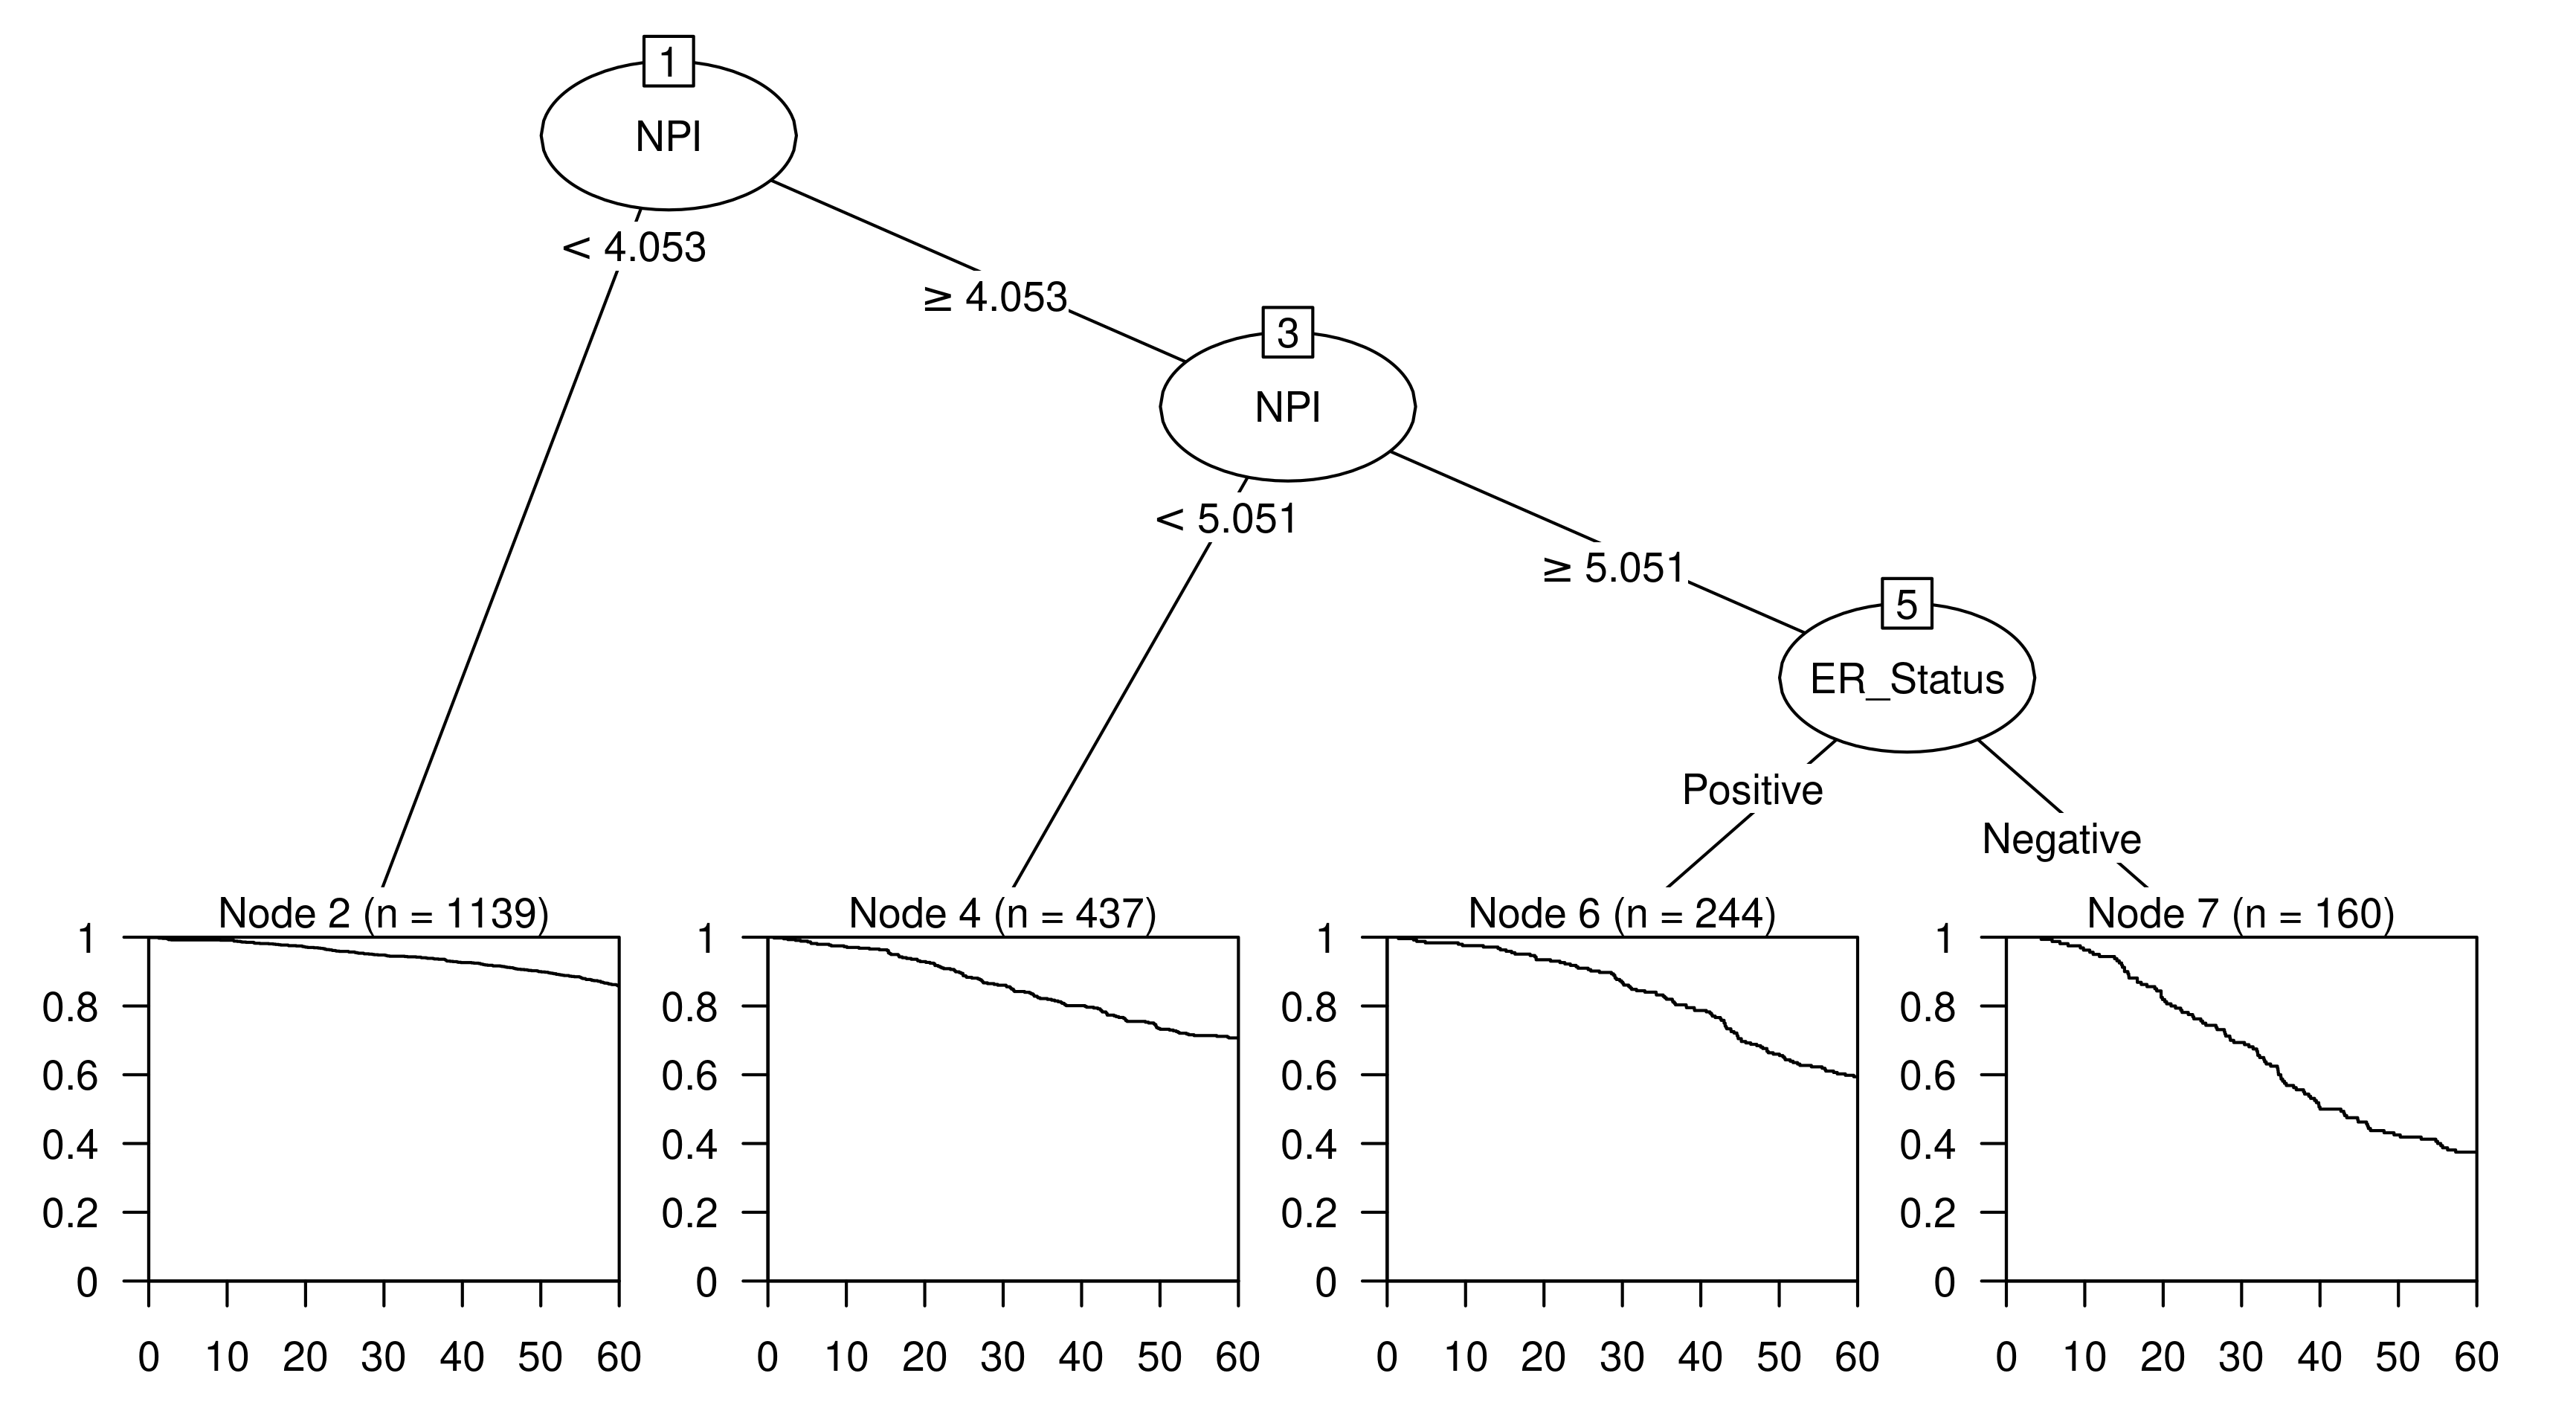
\includegraphics[width=1\textwidth]{../figures/Appendices/Appendix_B/Clin_PartyKit_Survival_Burden_FiveYearOS_INTCLUST.png}
\end{subfigure}

\vspace{2cm}

\begin{subfigure}{\textwidth}
\subcaption{}
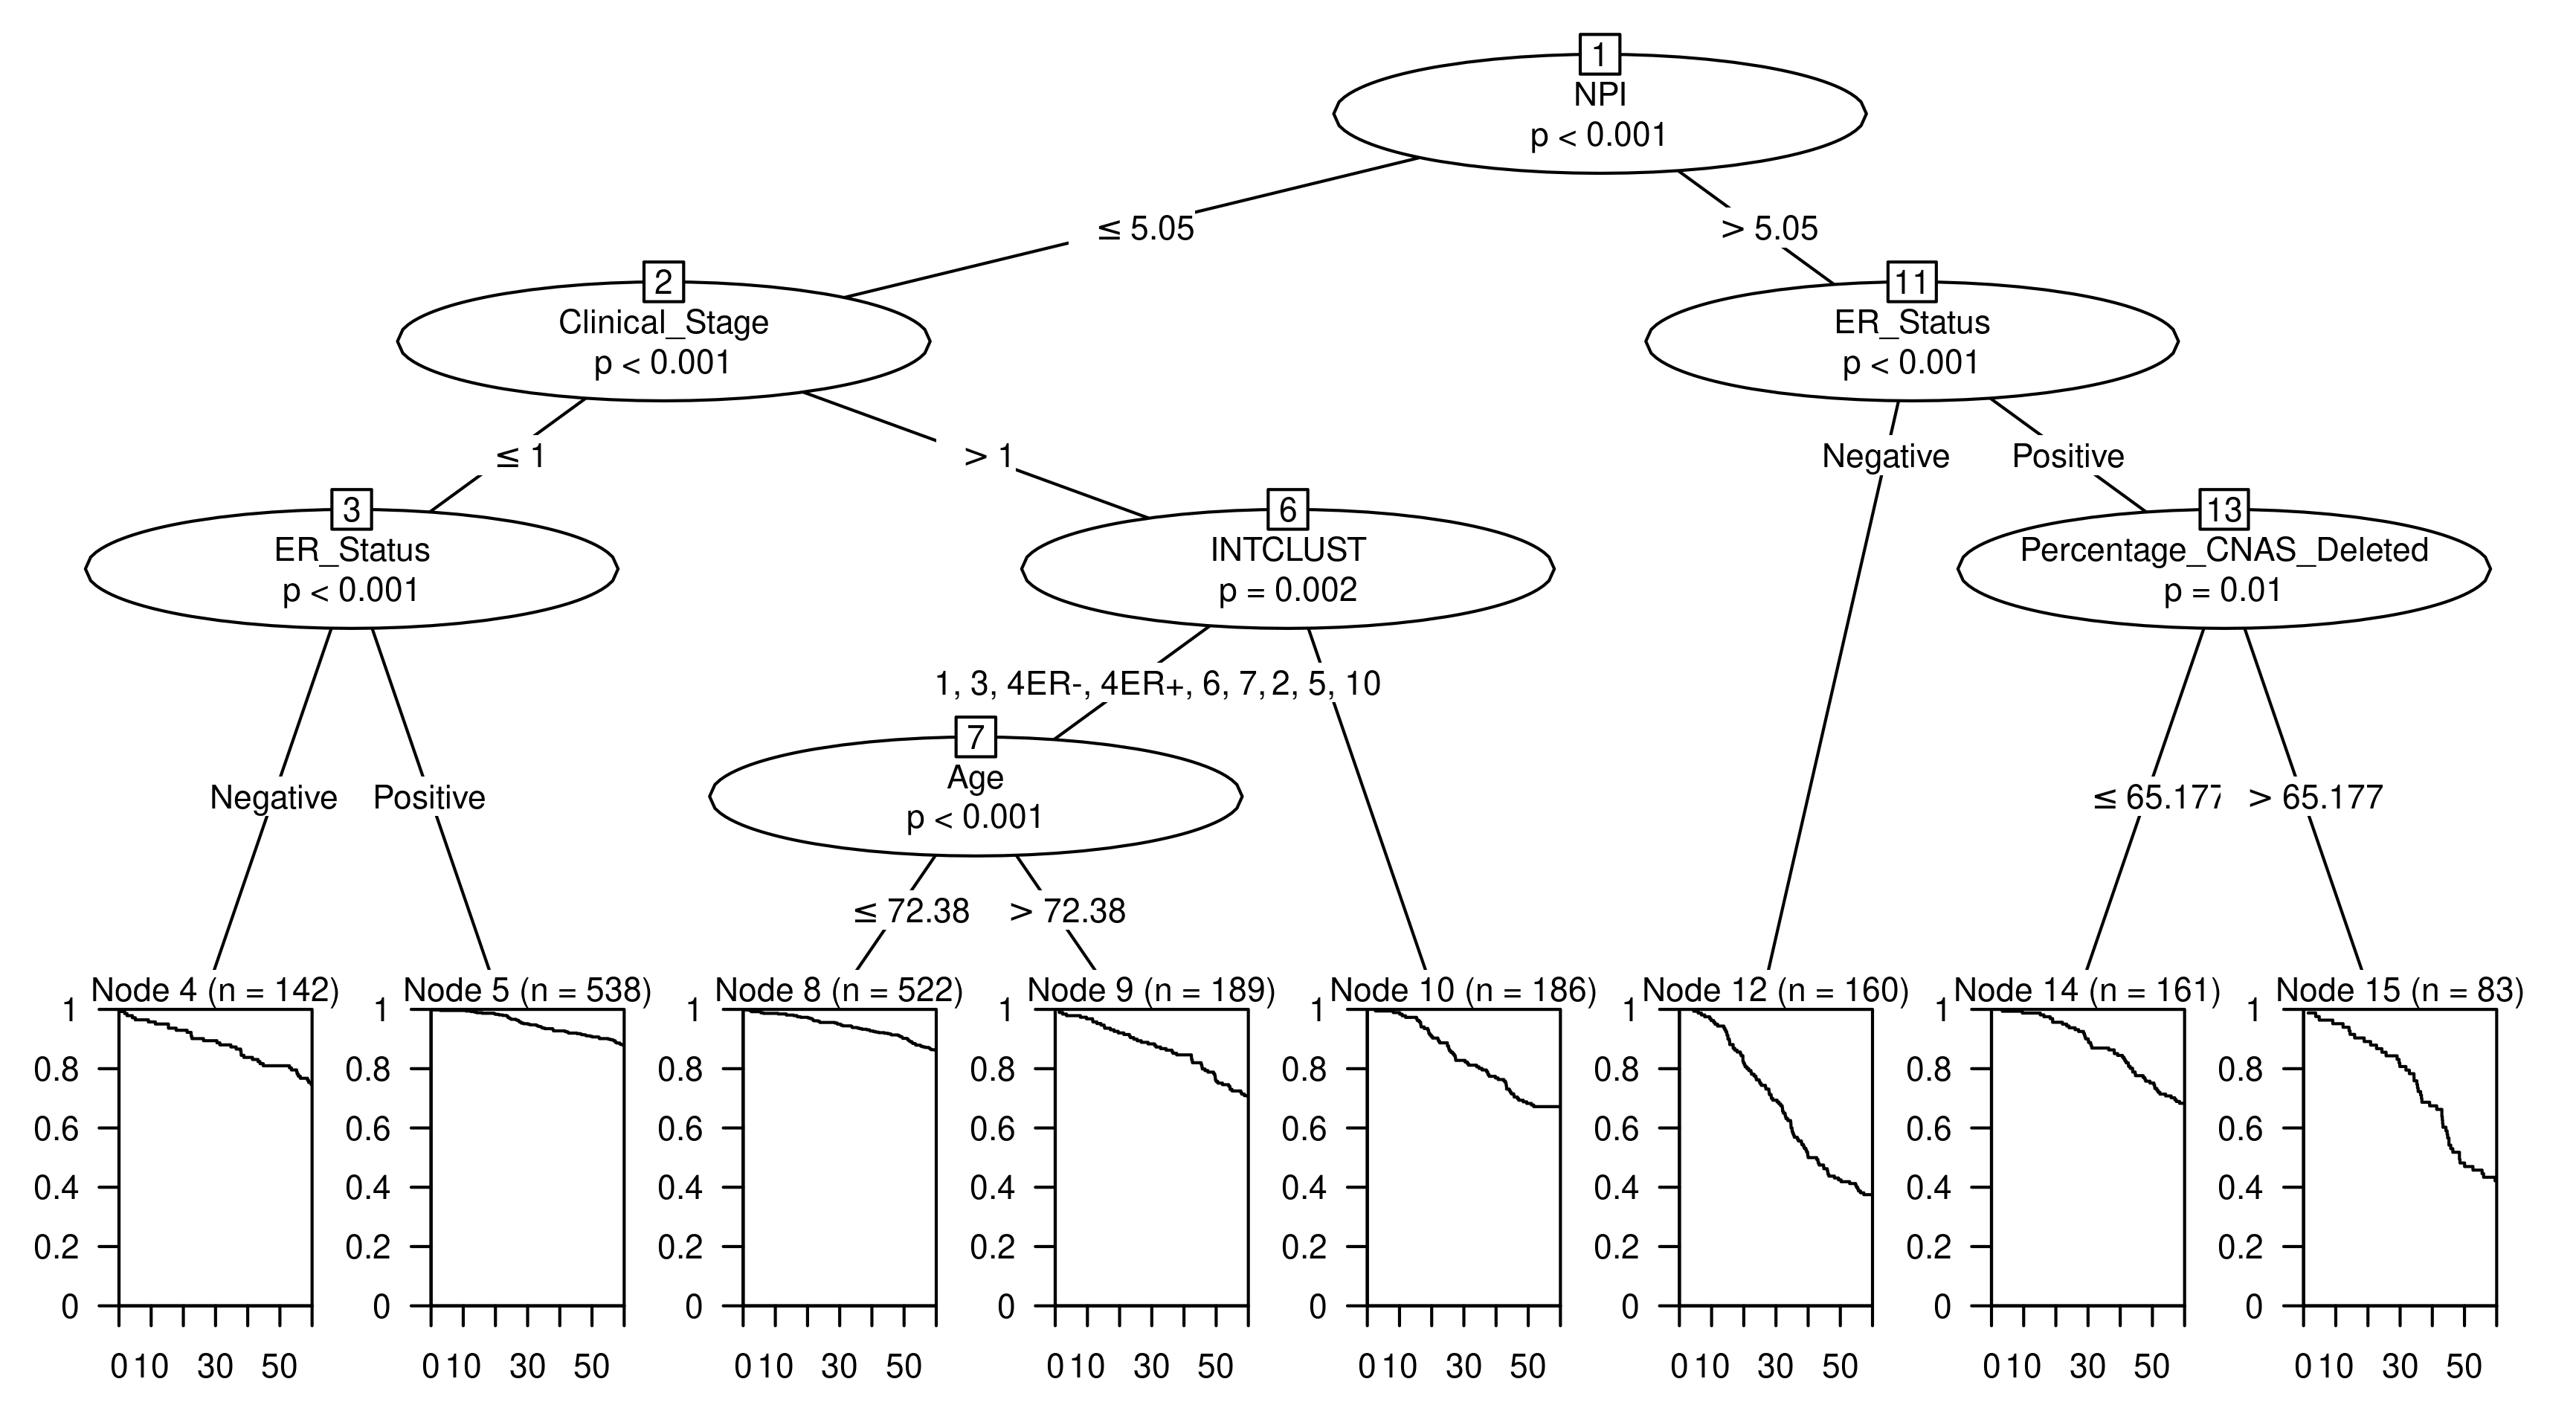
\includegraphics[width=1\textwidth]{../figures/Appendices/Appendix_B/Clin_Ctree_Survival_Burden_FiveYearOS_INTCLUST.png}
\end{subfigure}

\vspace{1cm}

\caption[Recursive partitioning survival trees for five-year overall survival using INTCLUST, the six CNA Burden metrics and a number of clinical variables as candidate predictors.]{Recursive partitioning survival trees for five-year overall survival using INTCLUST, the six CNA Burden metrics and a number of clinical variables as candidate predictors. (A) Trees fitted using the rpart algorithm and (B) trees fitted using the ctree algorithm.}
\end{figure}

\begin{figure}[!htb]
\centering

\vspace{1cm}

\begin{subfigure}{\textwidth}
\subcaption{}
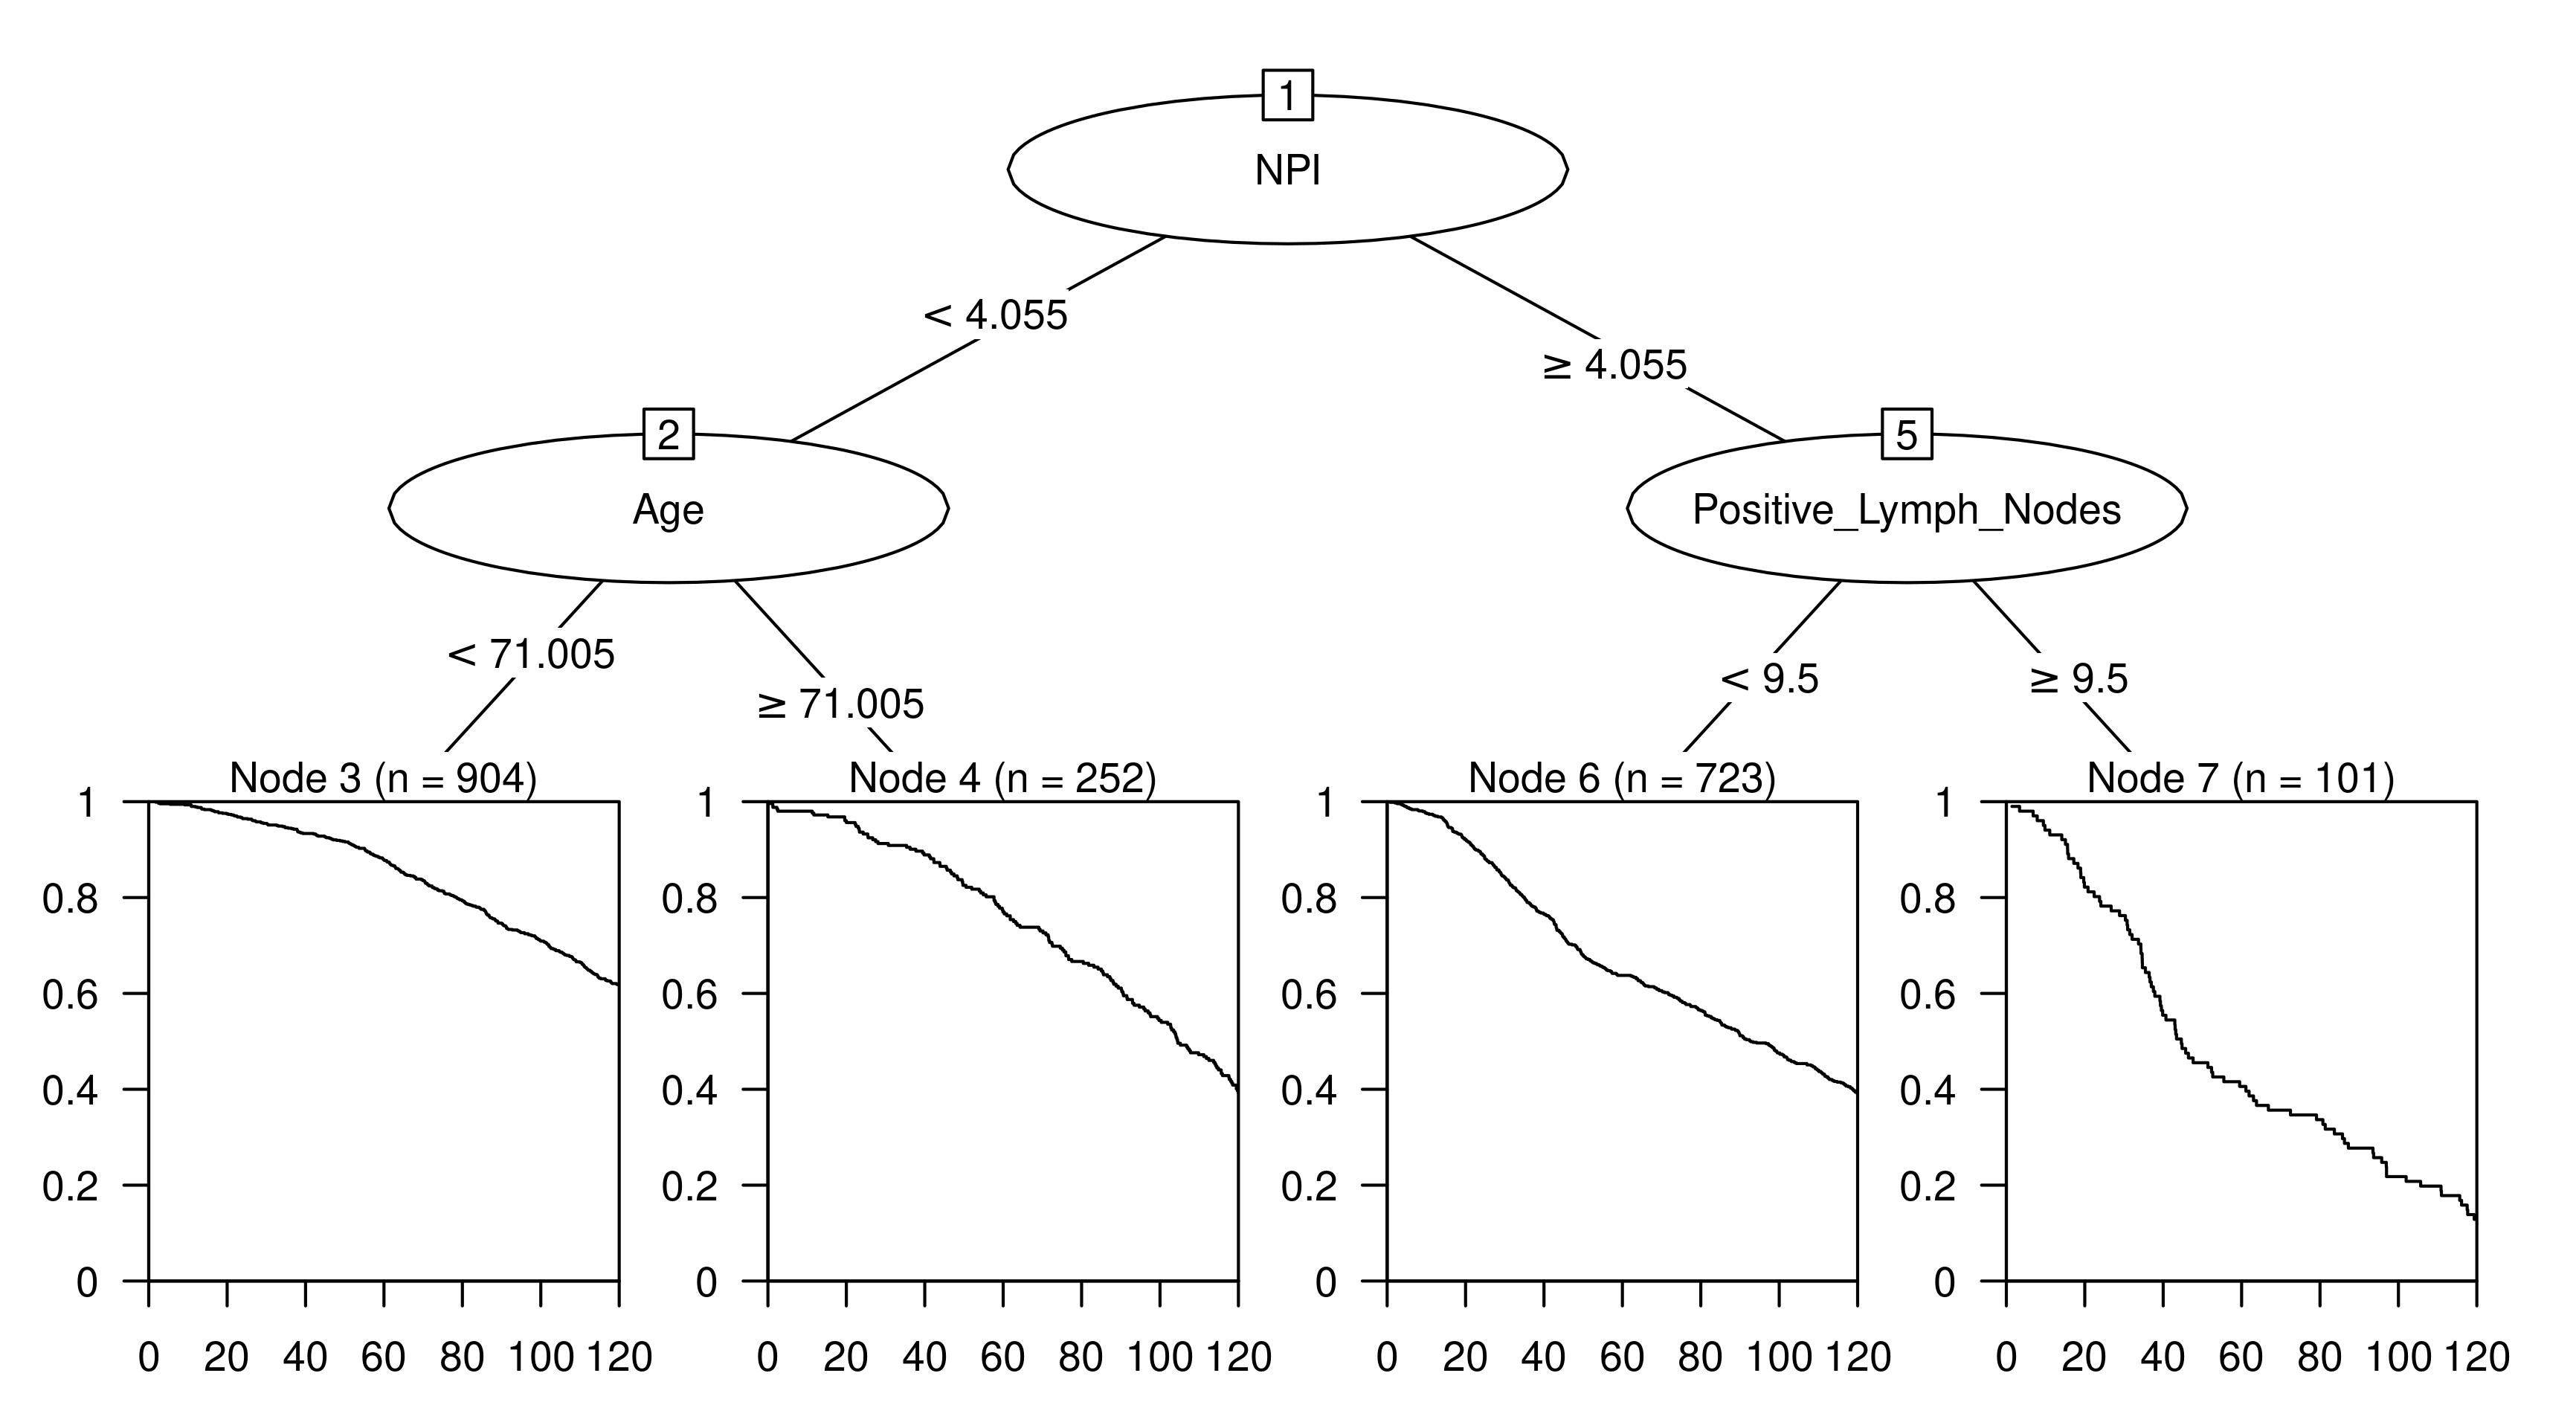
\includegraphics[width=1\textwidth]{../figures/Appendices/Appendix_B/Clin_PartyKit_Survival_Burden_TenYearOS_INTCLUST.png}
\end{subfigure}

\vspace{2cm}

\begin{subfigure}{\textwidth}
\subcaption{}
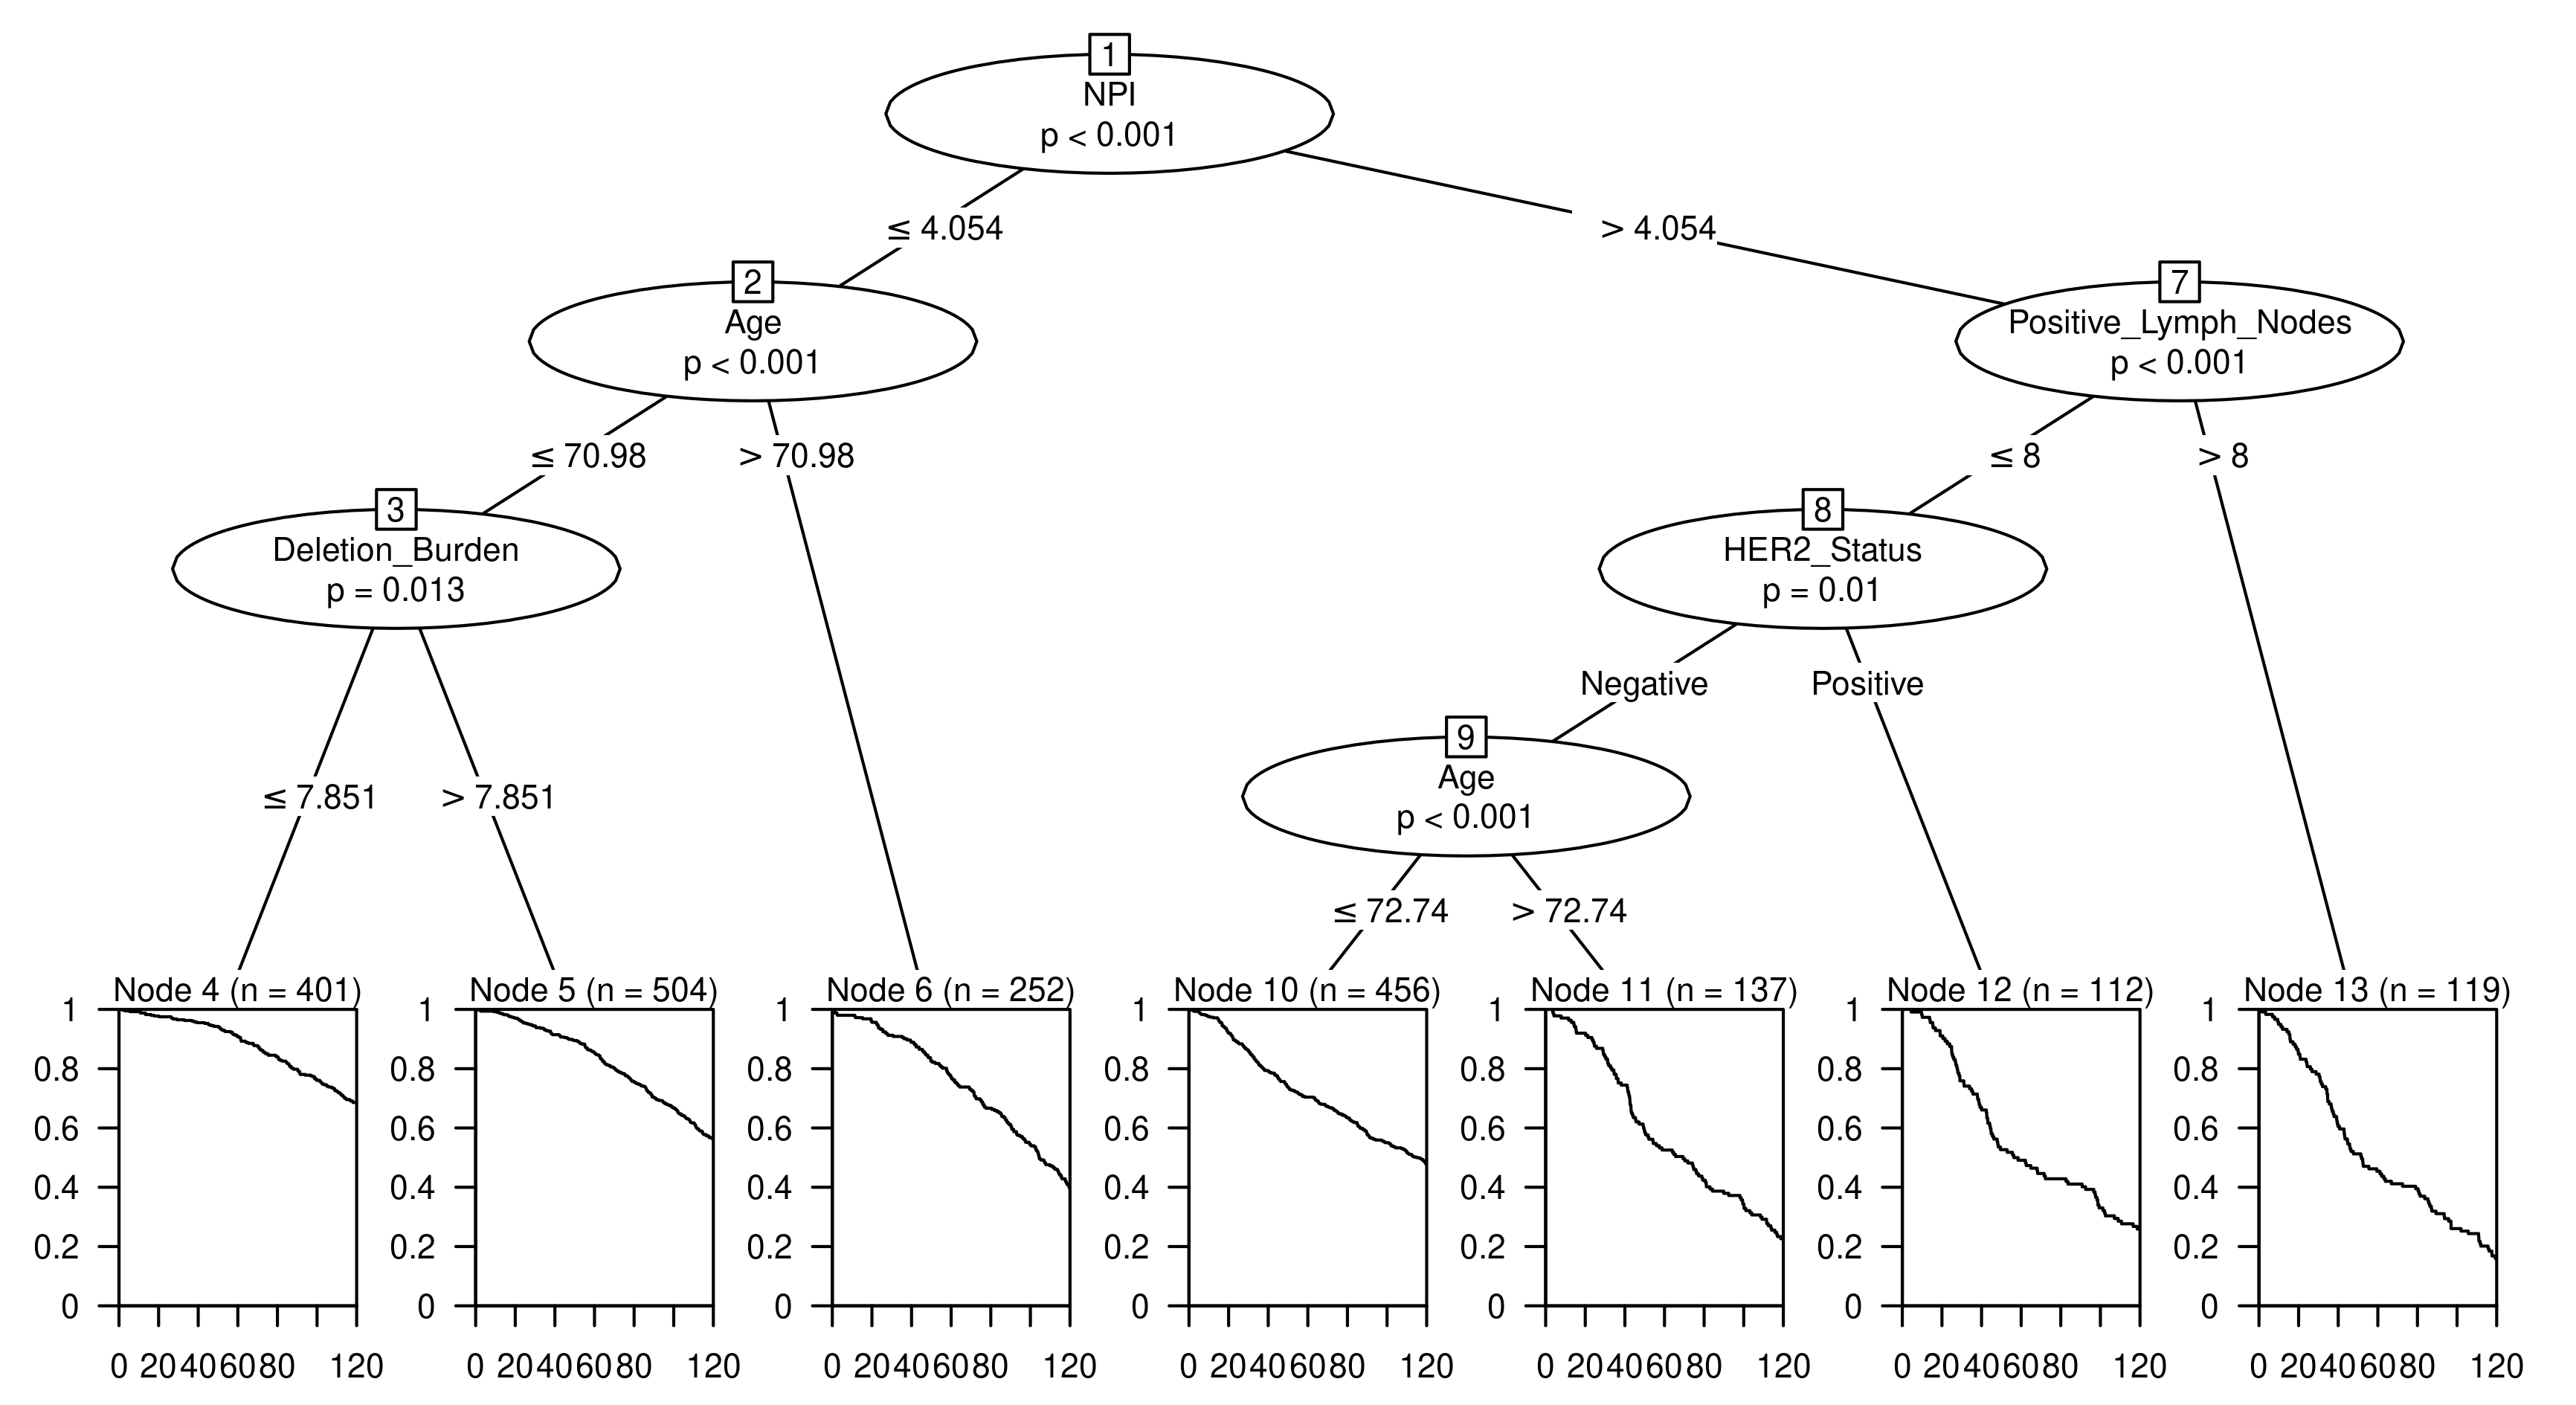
\includegraphics[width=1\textwidth]{../figures/Appendices/Appendix_B/Clin_Ctree_Survival_Burden_TenYearOS_INTCLUST.png}
\end{subfigure}

\vspace{1cm}

\caption[Recursive partitioning survival trees for ten-year overall survival using INTCLUST, the six CNA Burden metrics and a number of clinical variables as candidate predictors.]{Recursive partitioning survival trees for ten-year overall survival using INTCLUST, the six CNA Burden metrics and a number of clinical variables as candidate predictors. (A) Trees fitted using the rpart algorithm and (B) trees fitted using the ctree algorithm.}
\end{figure}

% Chromosome arm CNA metrics 
% OS using PAM50 Subtype and the 42 CNA Score metrics as candidate predictors
\begin{figure}[!htb]
\centering

\vspace{0.5cm}

\begin{subfigure}{\textwidth}
\subcaption{}
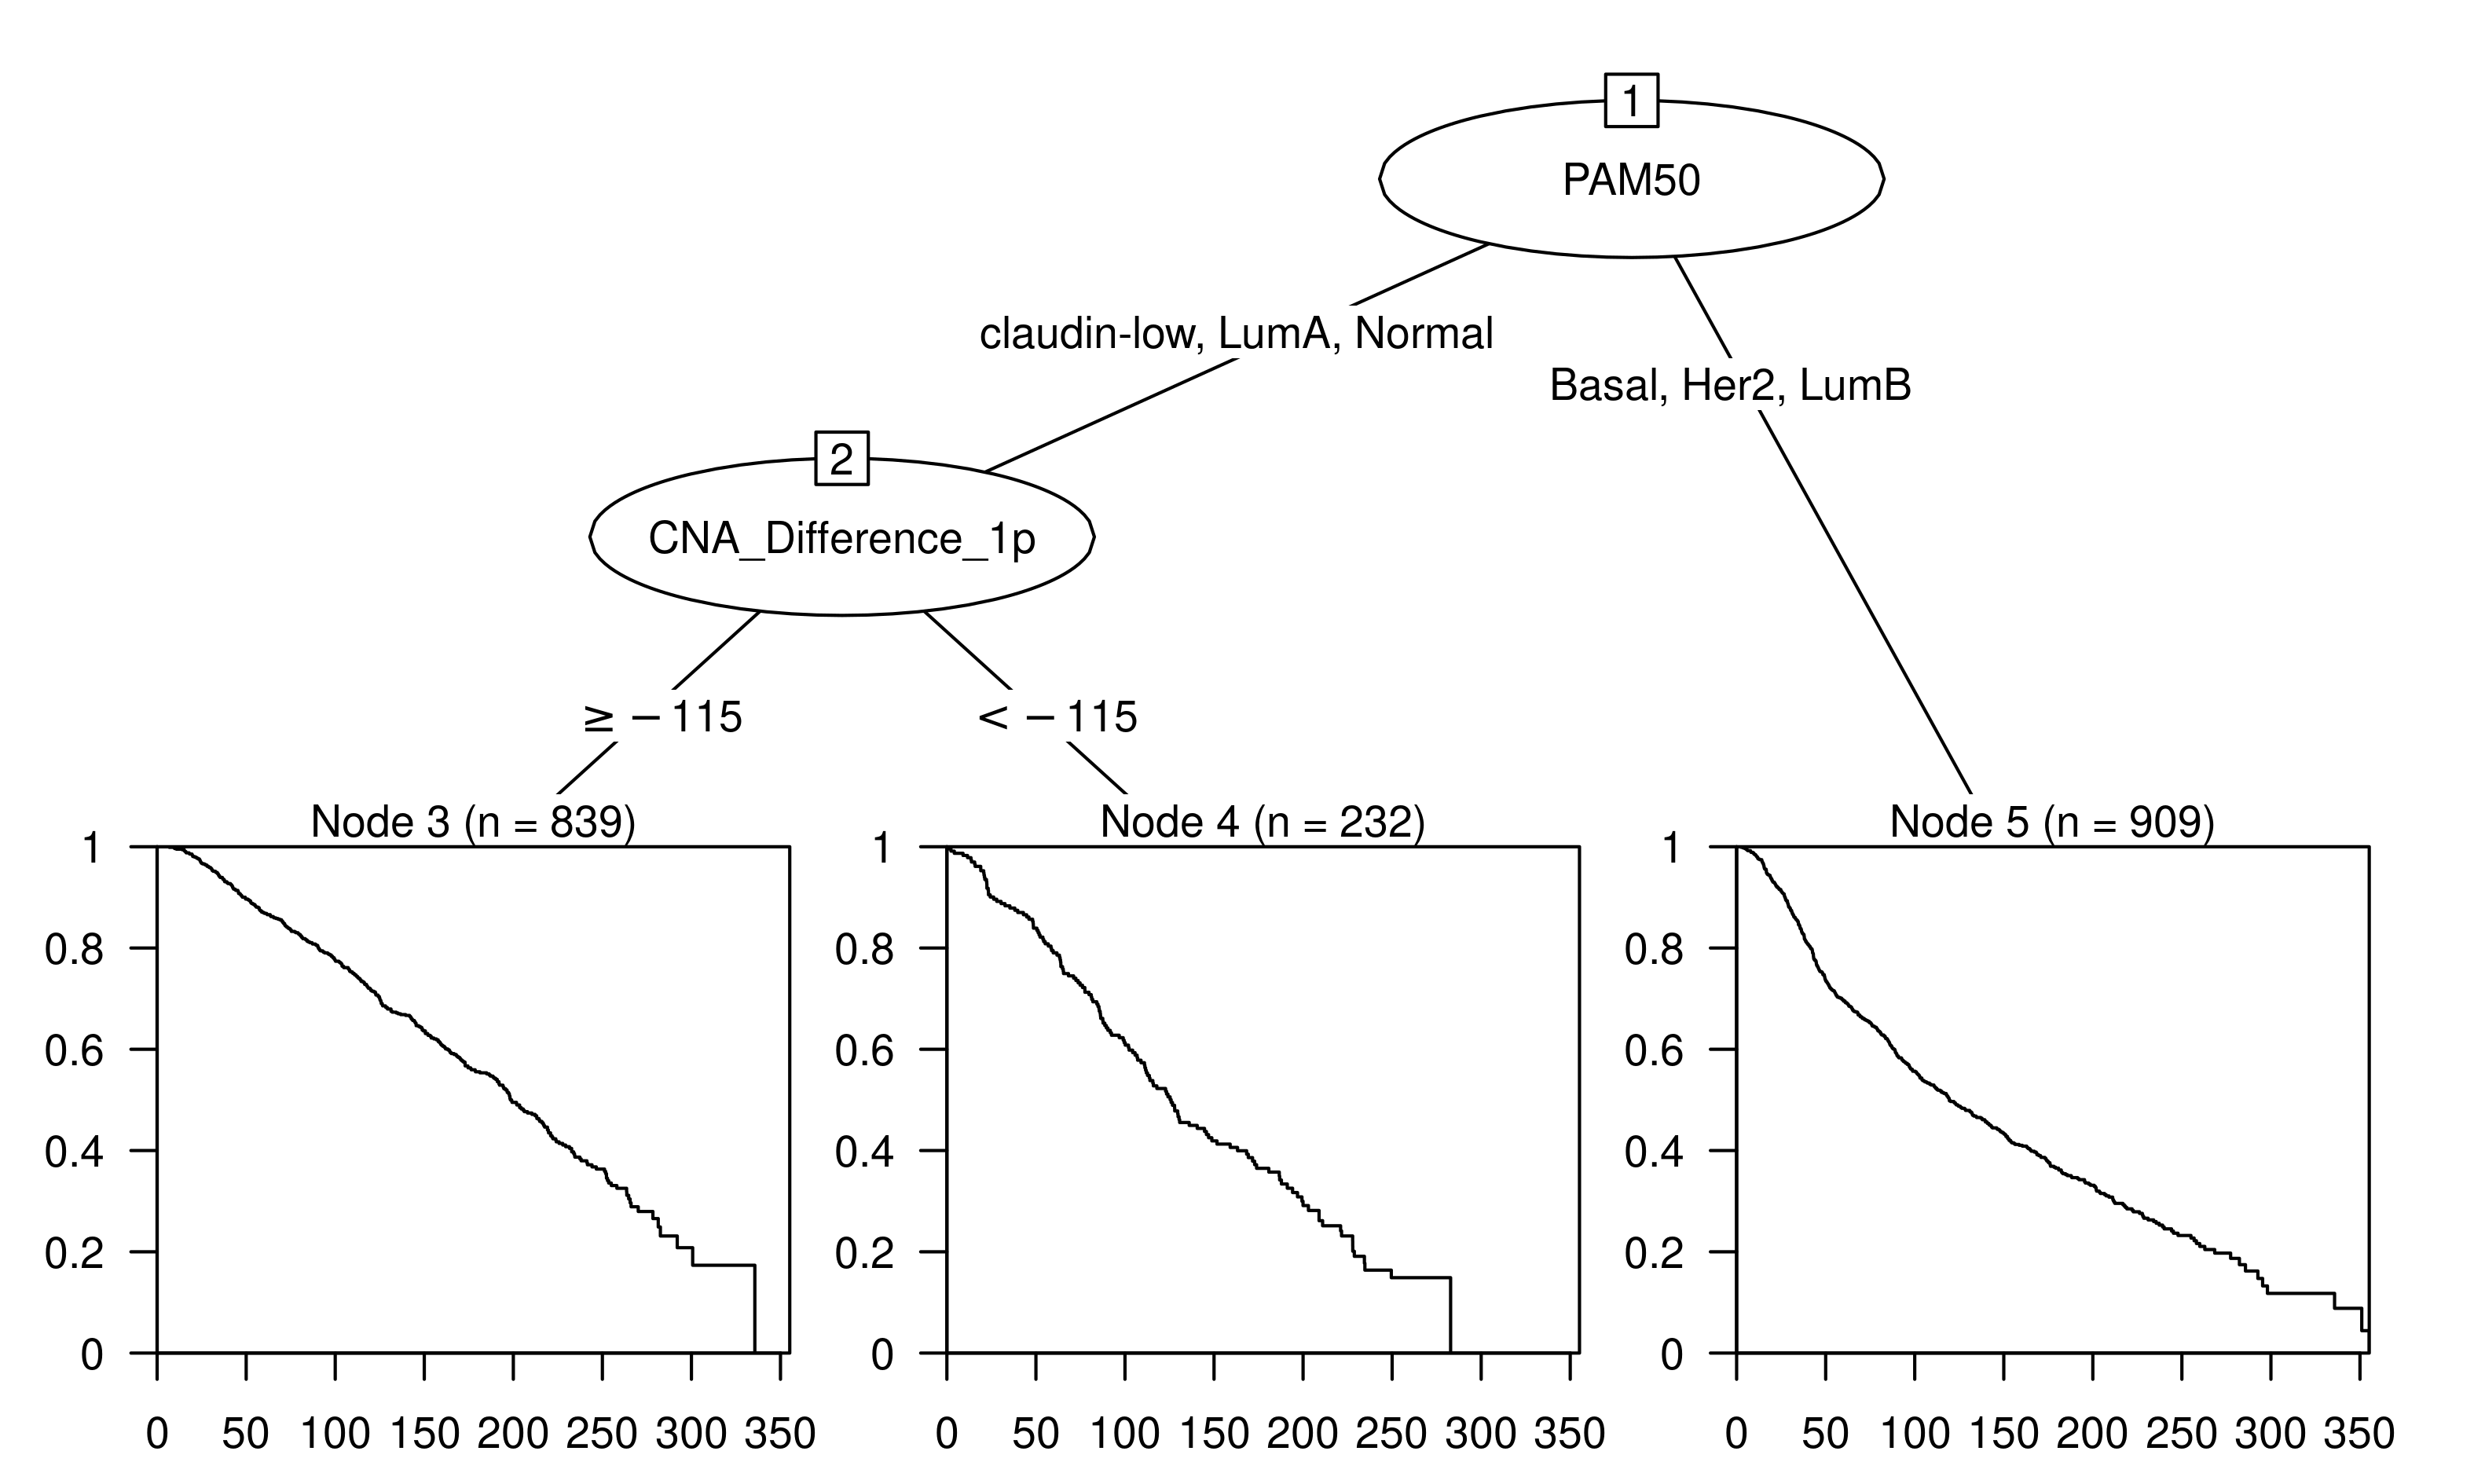
\includegraphics[width=1\textwidth]{../figures/Appendices/Appendix_B/PA_PartyKit_Survival_Score_OS_PAM50.png}
\end{subfigure}

\vspace{2cm}

\begin{subfigure}{\textwidth}
\subcaption{}
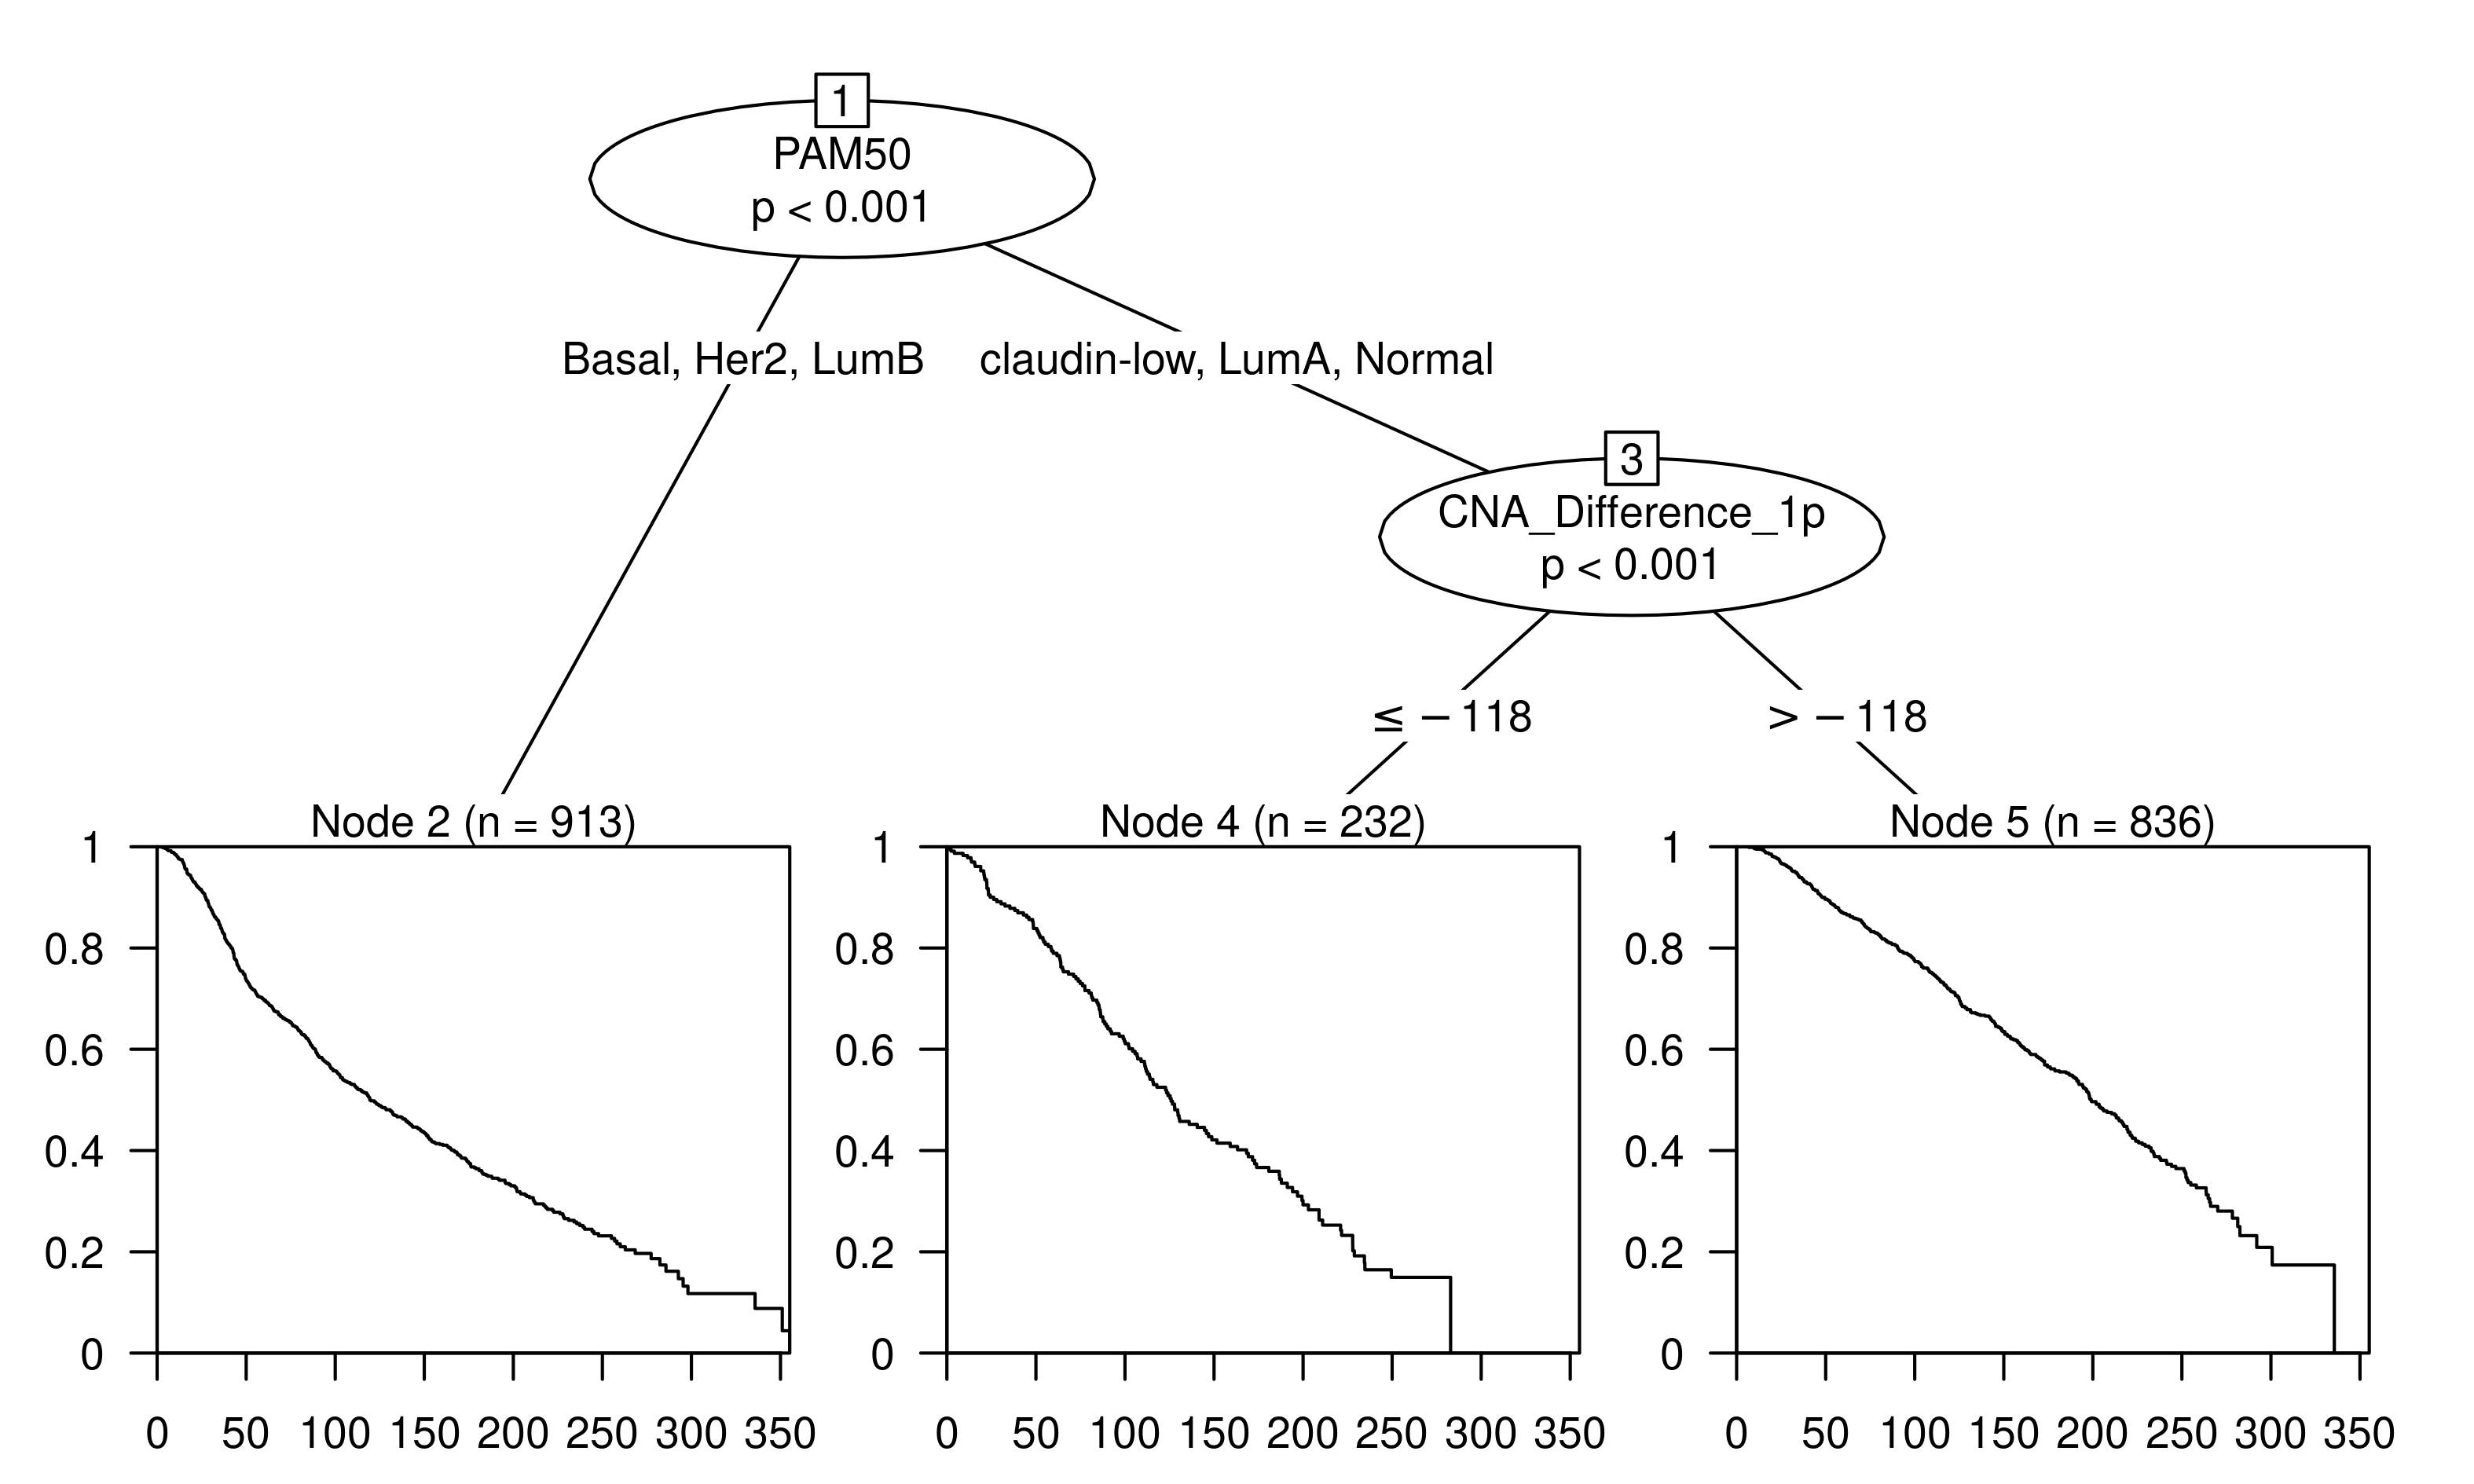
\includegraphics[width=1\textwidth]{../figures/Appendices/Appendix_B/PA_Ctree_Survival_Score_OS_PAM50.png}
\end{subfigure}

\vspace{0.5cm}

\caption[Recursive partitioning survival trees for overall survival using PAM50 and the 42 chromosome arm CNA Score metrics as candidate predictors.]{Recursive partitioning survival trees for overall survival using PAM50 and the 42 chromosome arm CNA Score metrics as candidate predictors. (A) Trees fitted using the rpart algorithm and (B) trees fitted using the ctree algorithm.}
\end{figure}

\begin{figure}[!htb]
\centering

\vspace{0.5cm}

\begin{subfigure}{\textwidth}
\subcaption{}
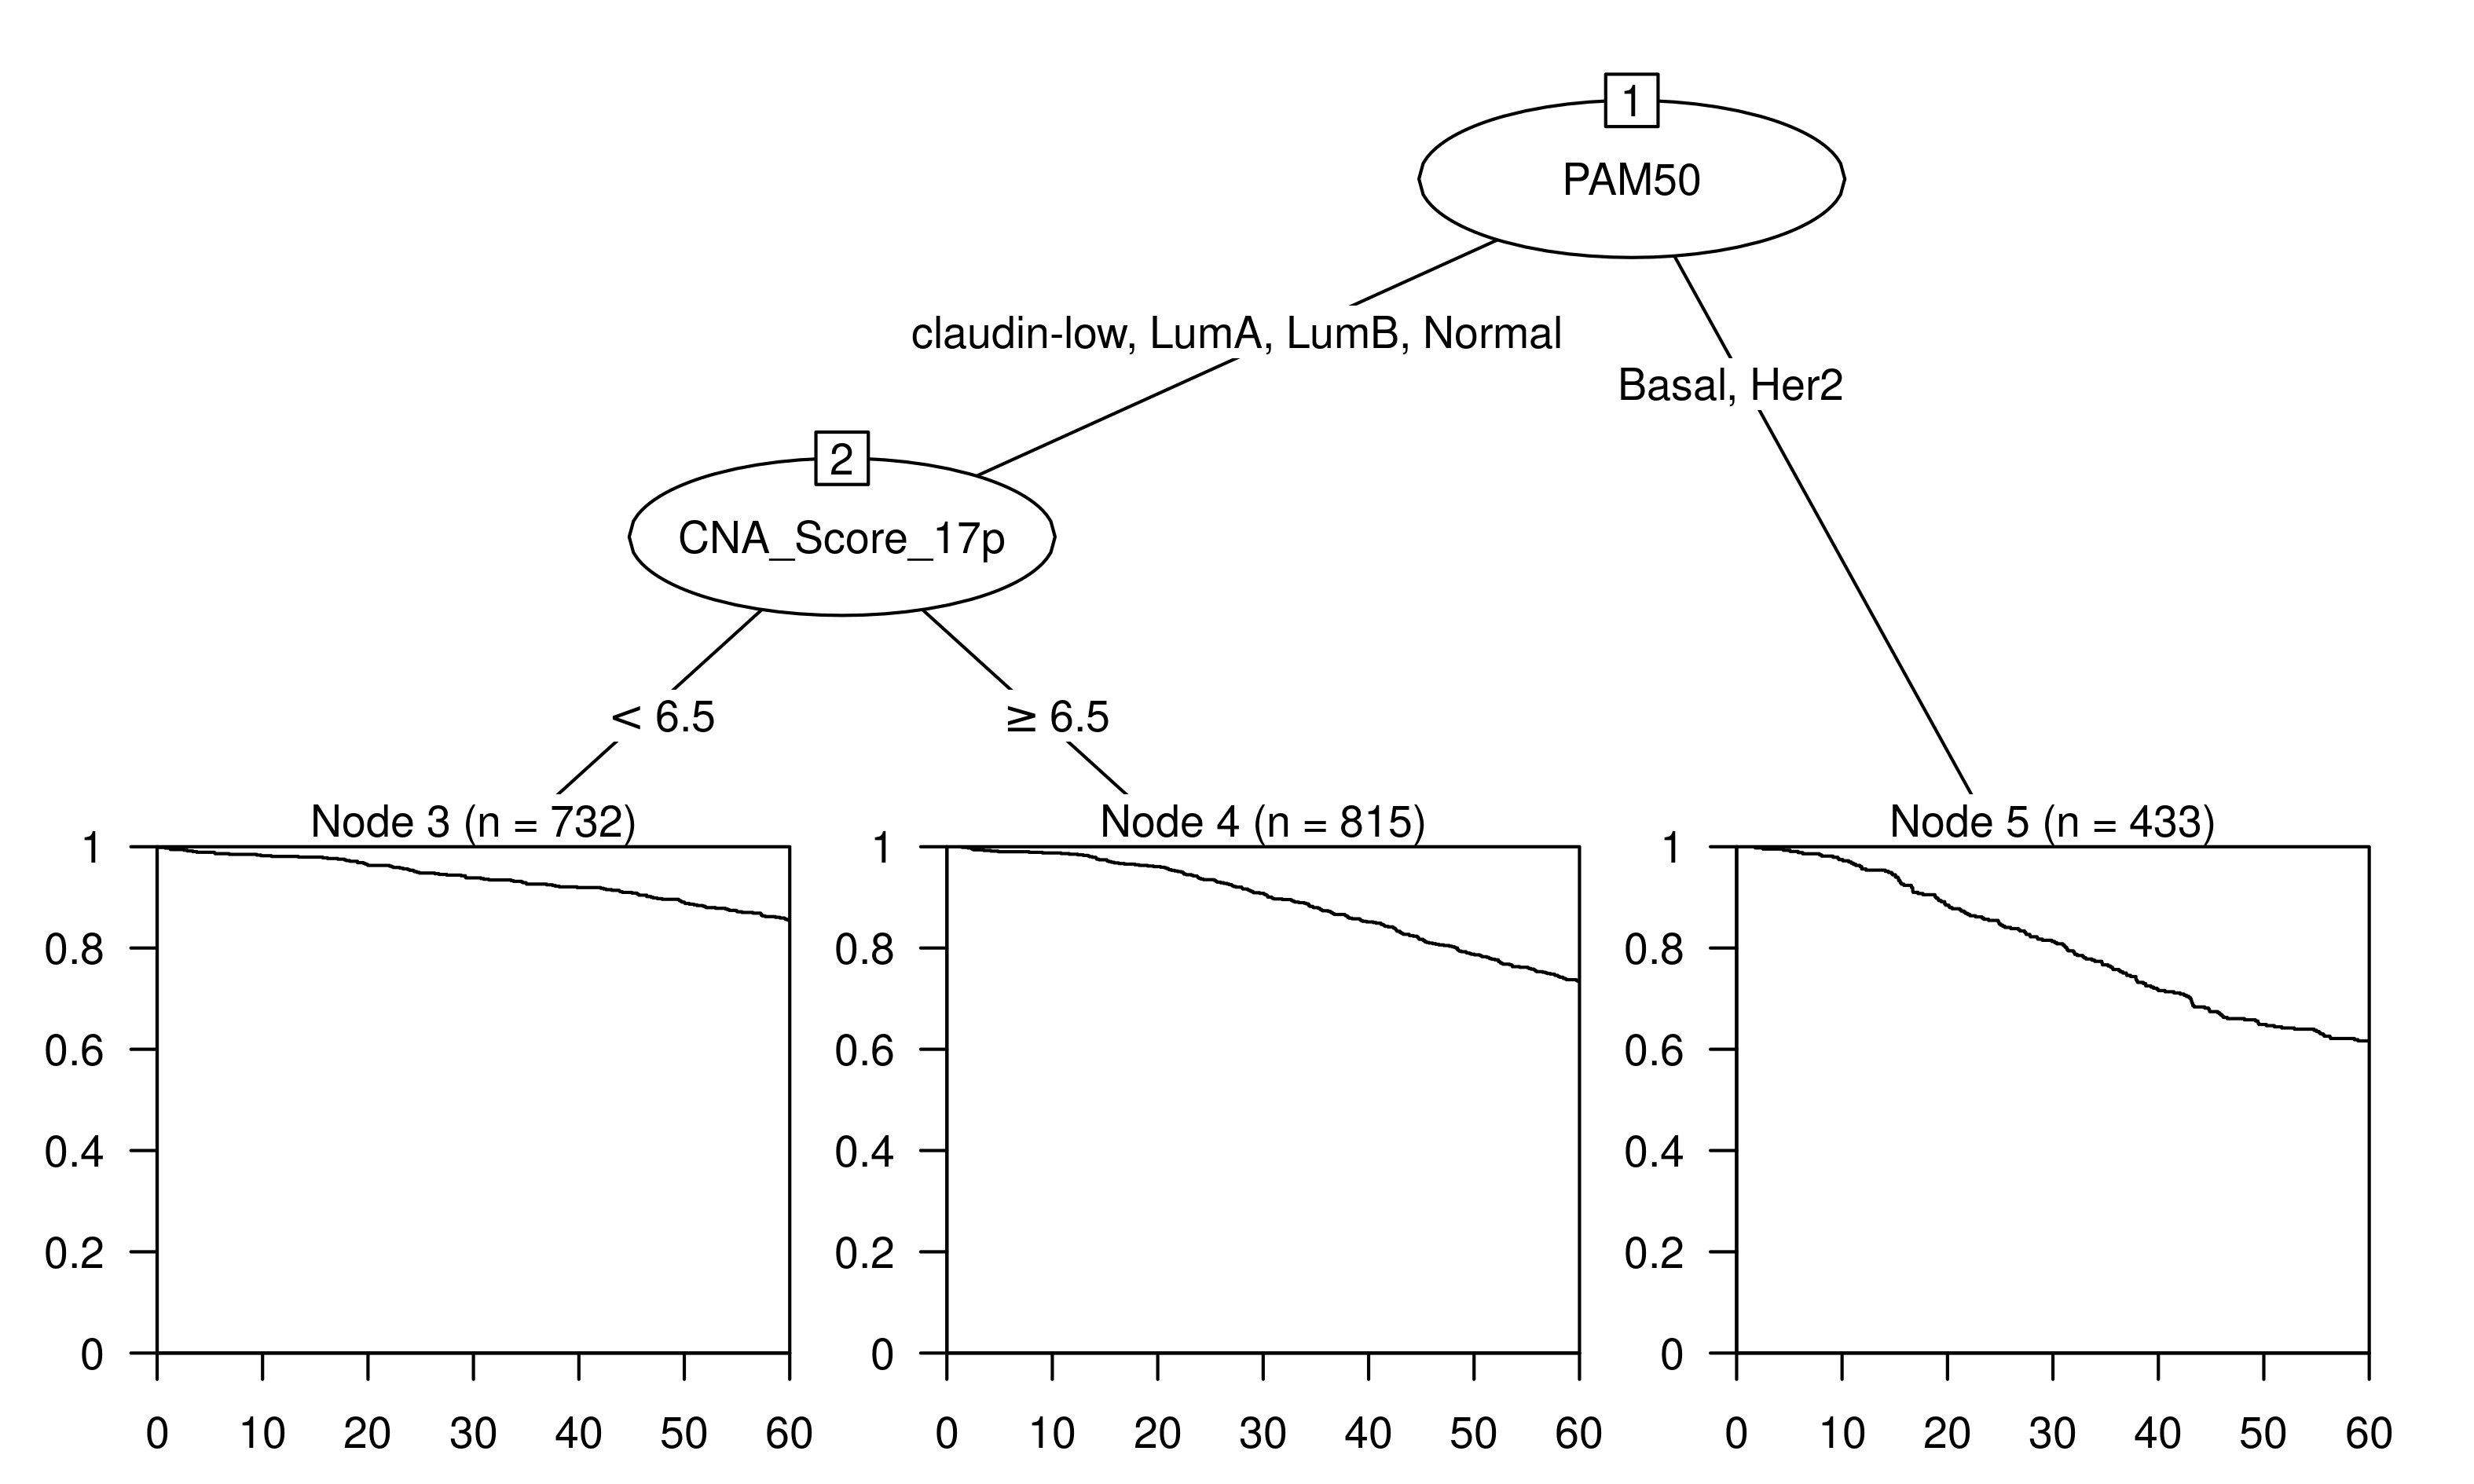
\includegraphics[width=1\textwidth]{../figures/Appendices/Appendix_B/PA_PartyKit_Survival_Score_FiveYearOS_PAM50.png}
\end{subfigure}

\vspace{2cm}

\begin{subfigure}{\textwidth}
\subcaption{}
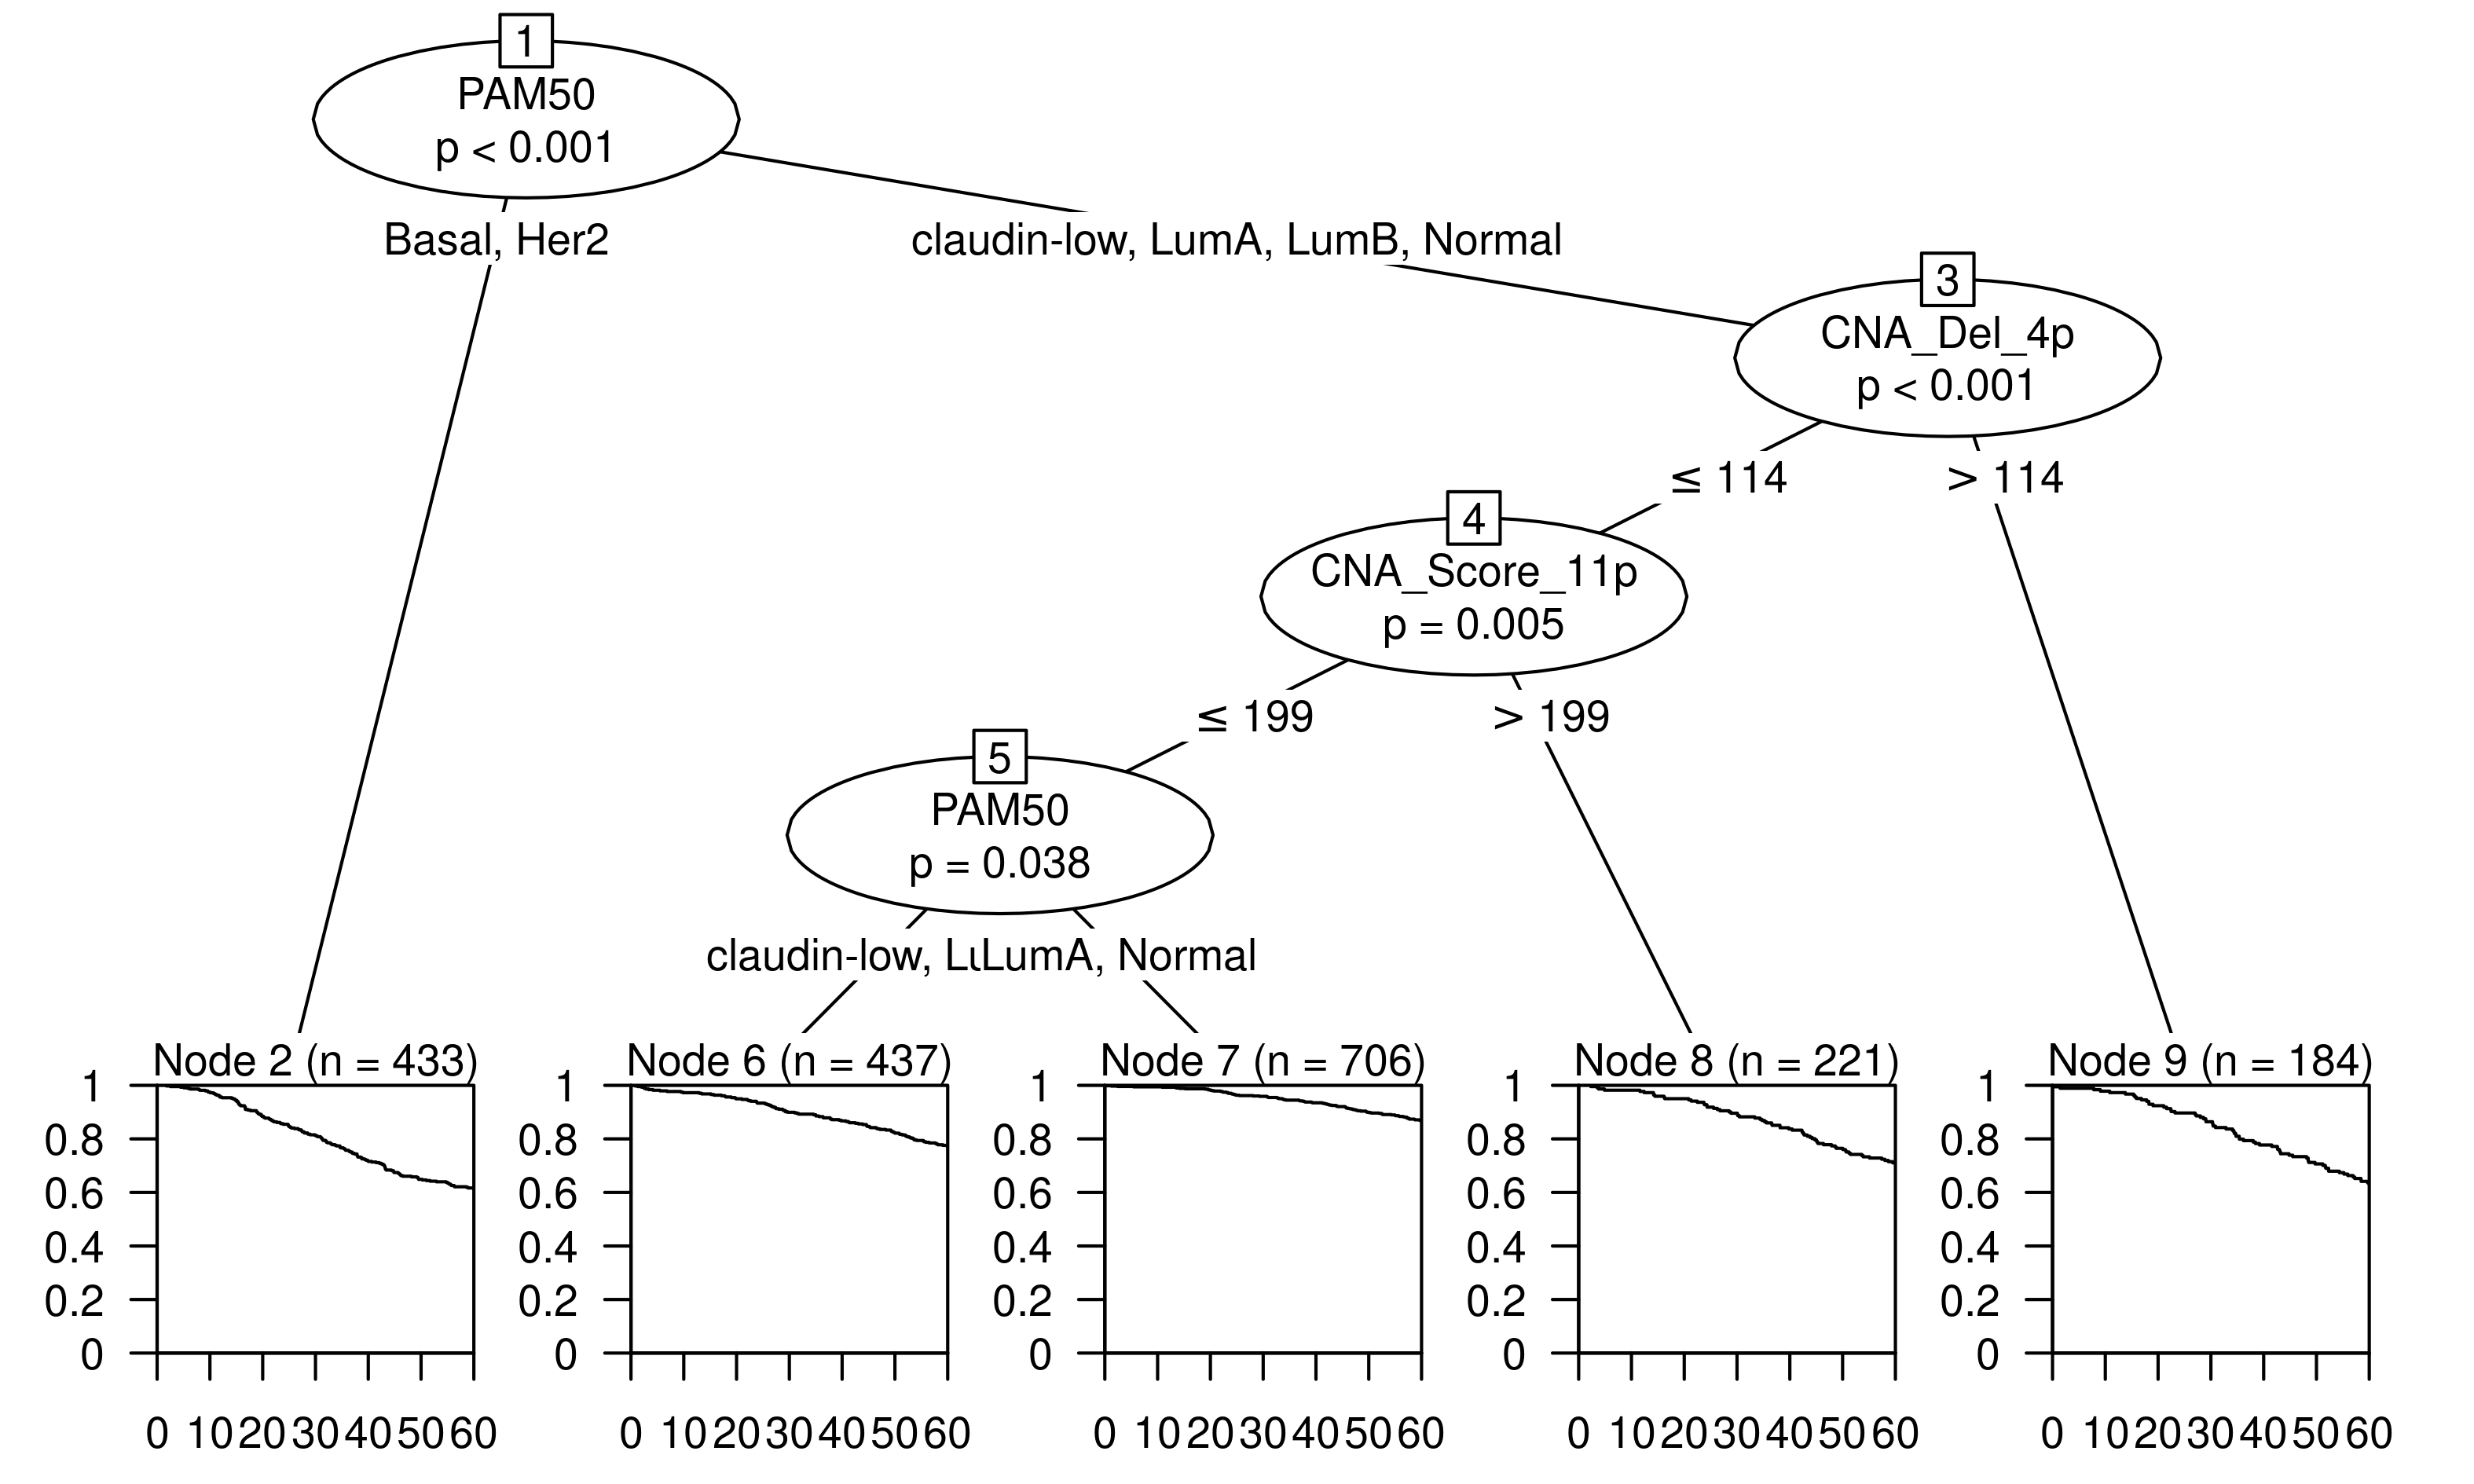
\includegraphics[width=1\textwidth]{../figures/Appendices/Appendix_B/PA_Ctree_Survival_Score_FiveYearOS_PAM50.png}
\end{subfigure}

\vspace{0.5cm}

\caption[Recursive partitioning survival trees for five-year overall survival using PAM50 and the 42 chromosome arm CNA Score metrics as candidate predictors.]{Recursive partitioning survival trees for five-year overall survival using PAM50 and the 42 chromosome arm CNA Score metrics as candidate predictors. (A) Trees fitted using the rpart algorithm and (B) trees fitted using the ctree algorithm.}
\end{figure}


\begin{figure}[!htb]
\centering

\vspace{0.5cm}

\begin{subfigure}{\textwidth}
\subcaption{}
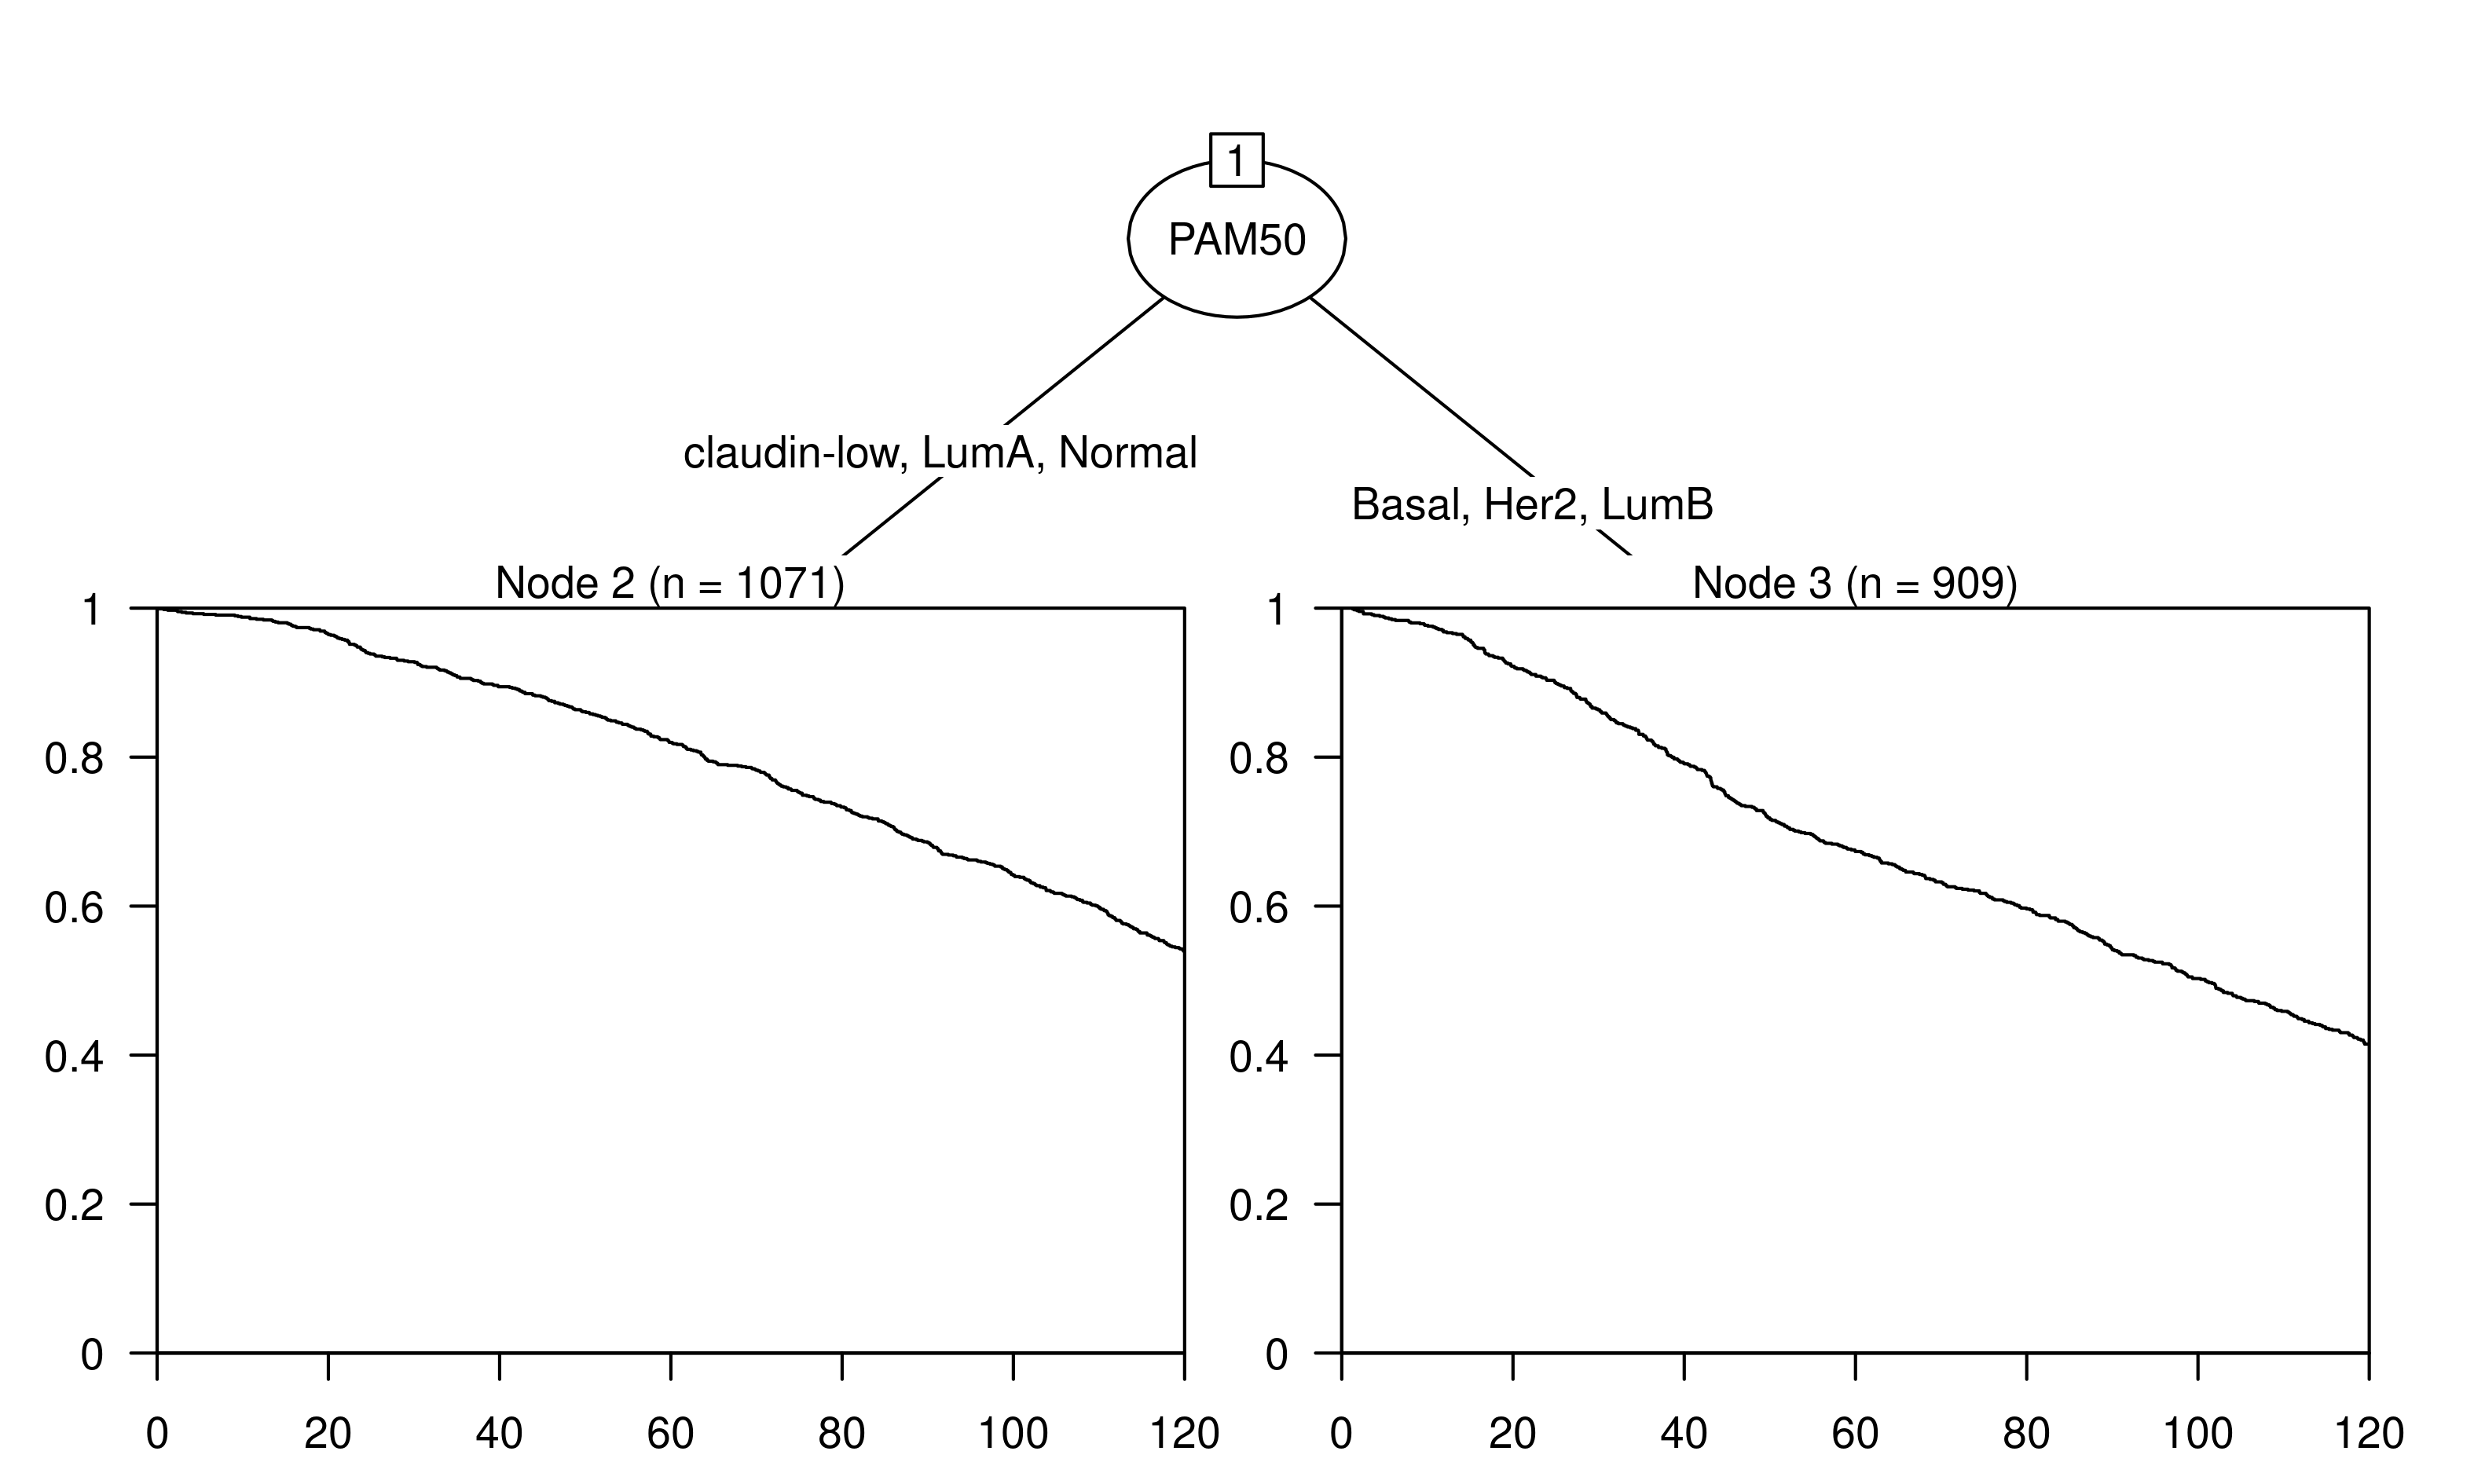
\includegraphics[width=1\textwidth]{../figures/Appendices/Appendix_B/PA_PartyKit_Survival_Score_TenYearOS_PAM50.png}
\end{subfigure}

\vspace{2cm}

\begin{subfigure}{\textwidth}
\subcaption{}
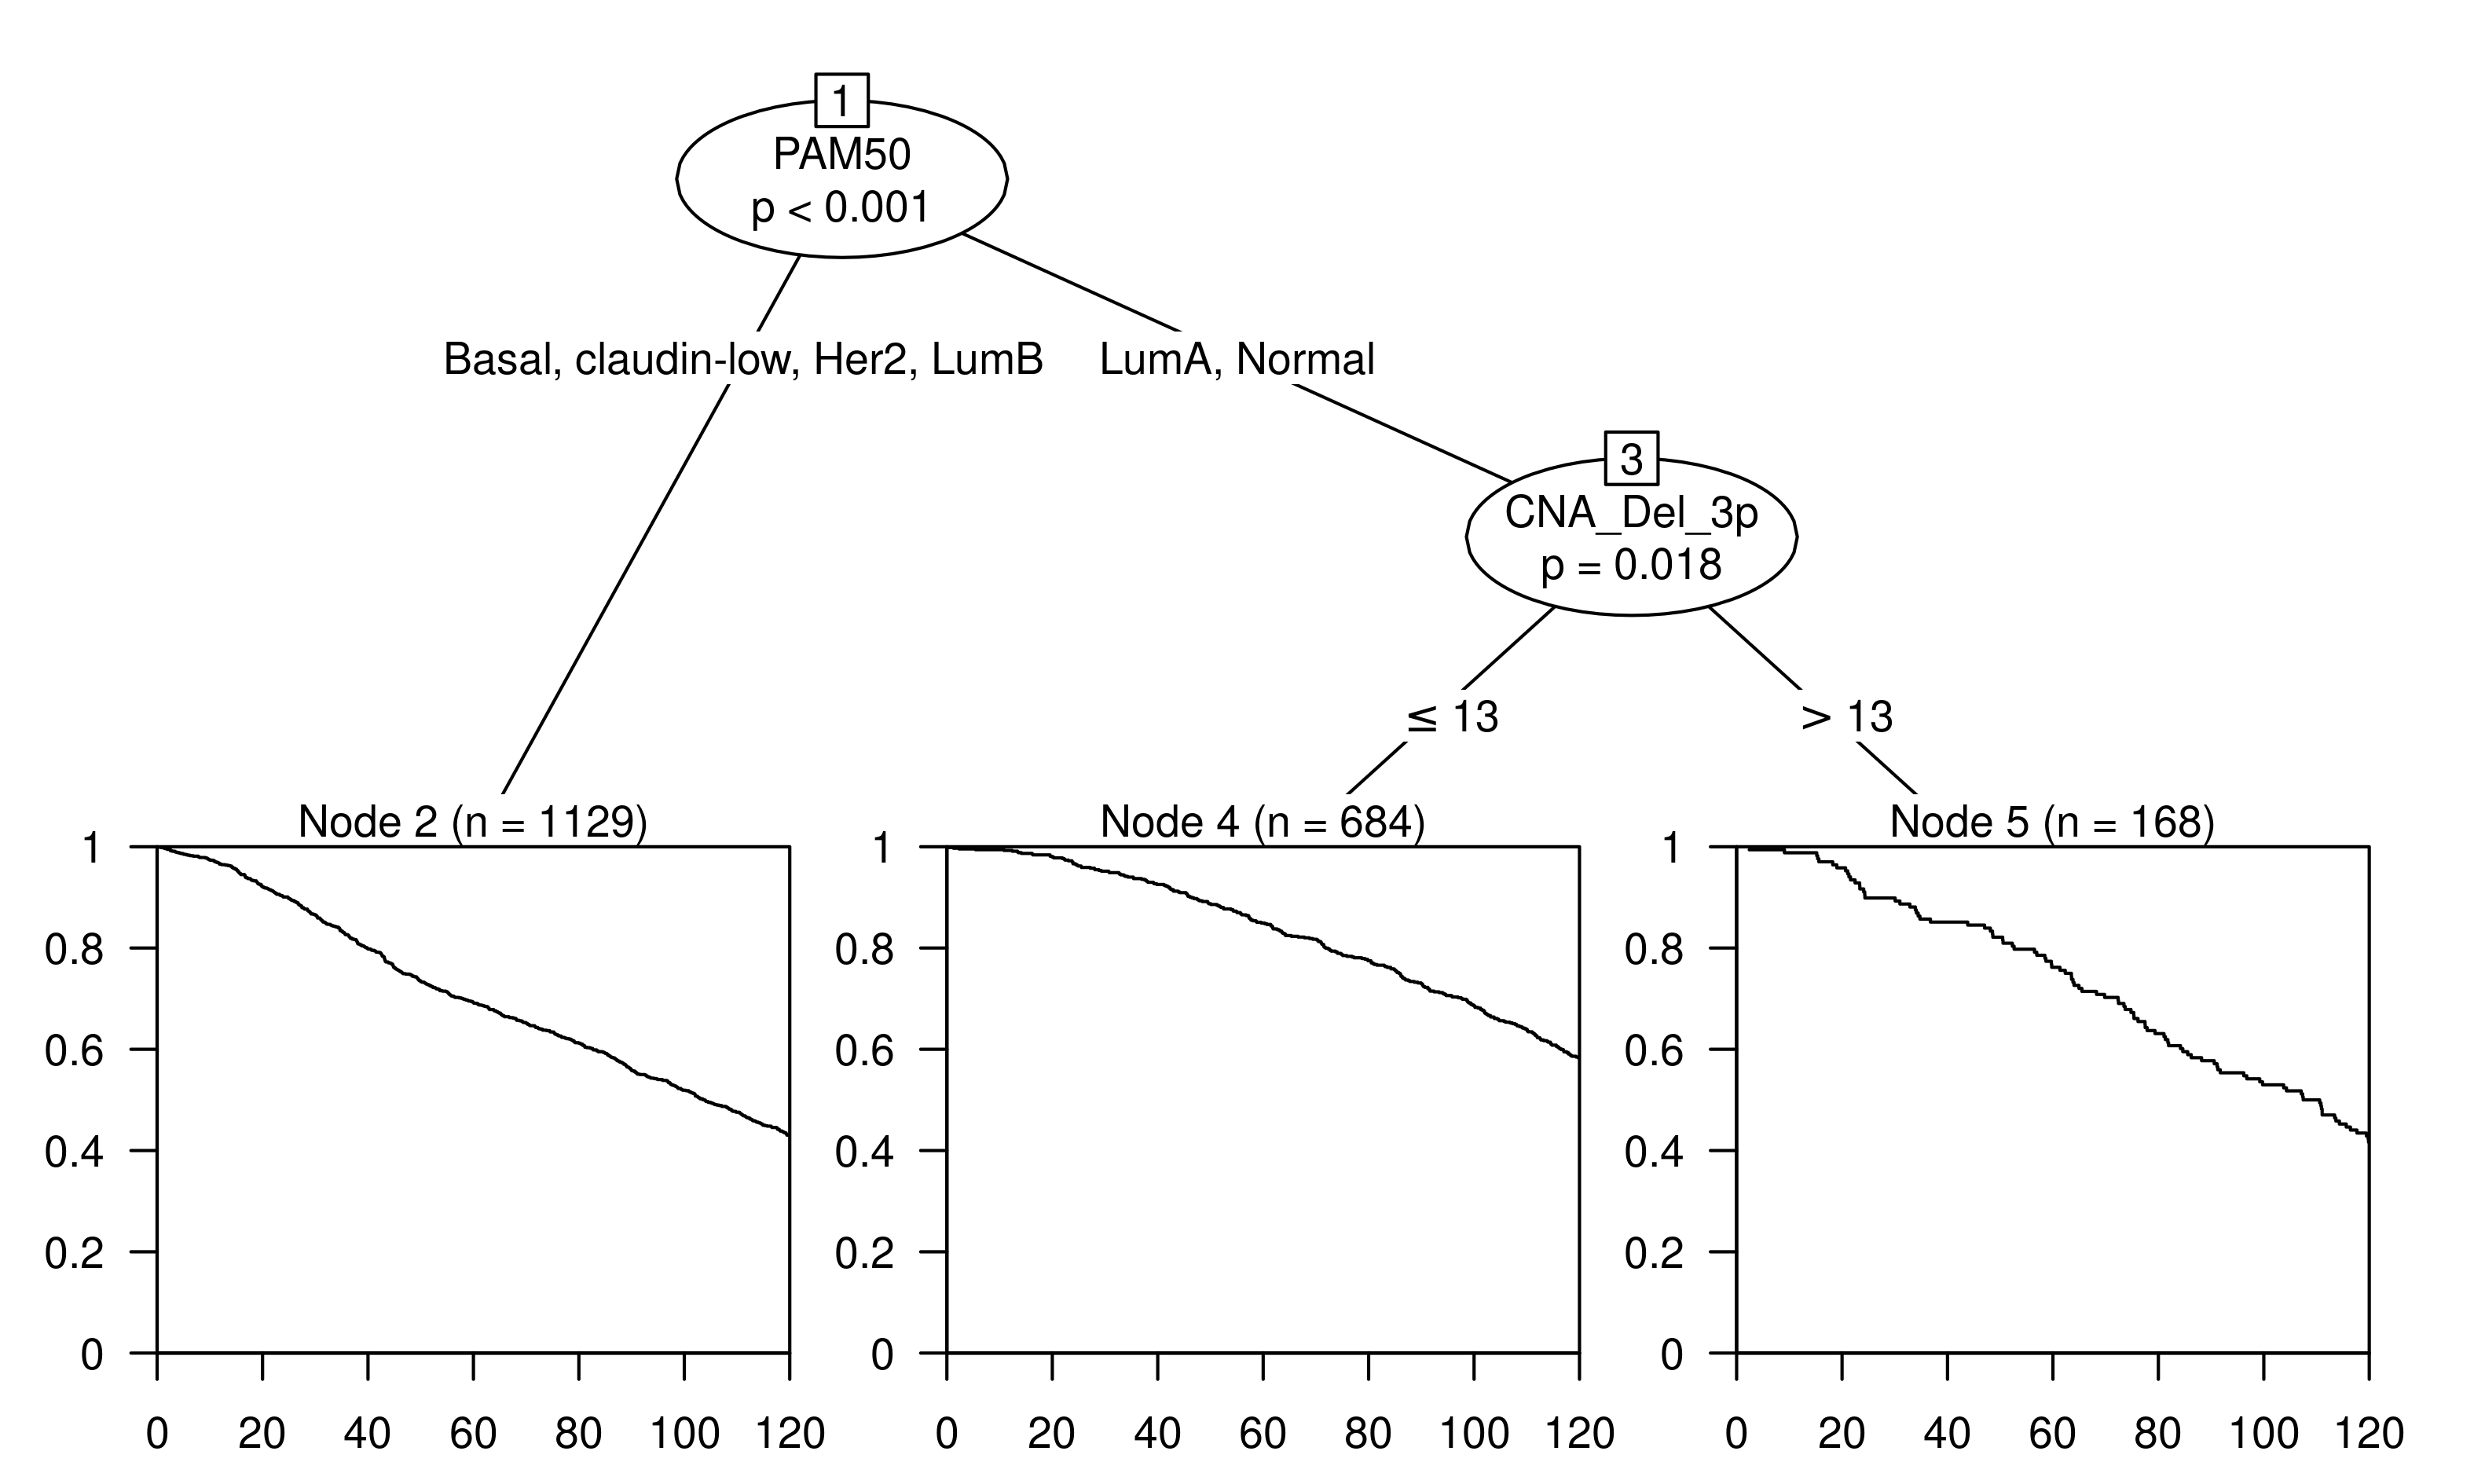
\includegraphics[width=1\textwidth]{../figures/Appendices/Appendix_B/PA_Ctree_Survival_Score_TenYearOS_PAM50.png}
\end{subfigure}

\vspace{0.5cm}

\caption[Recursive partitioning survival trees for five-year overall survival using PAM50 and the 42 chromosome arm CNA Score metrics as candidate predictors.]{Recursive partitioning survival trees for five-year overall survival using PAM50 and the 42 chromosome arm CNA Score metrics as candidate predictors. (A) Trees fitted using the rpart algorithm and (B) trees fitted using the ctree algorithm.}
\end{figure}

% OS using PAM50 Subtype and the 42 CNA Burden metrics as candidate predictors
\begin{figure}[!htb]
\centering

\vspace{0.5cm}

\begin{subfigure}{\textwidth}
\subcaption{}
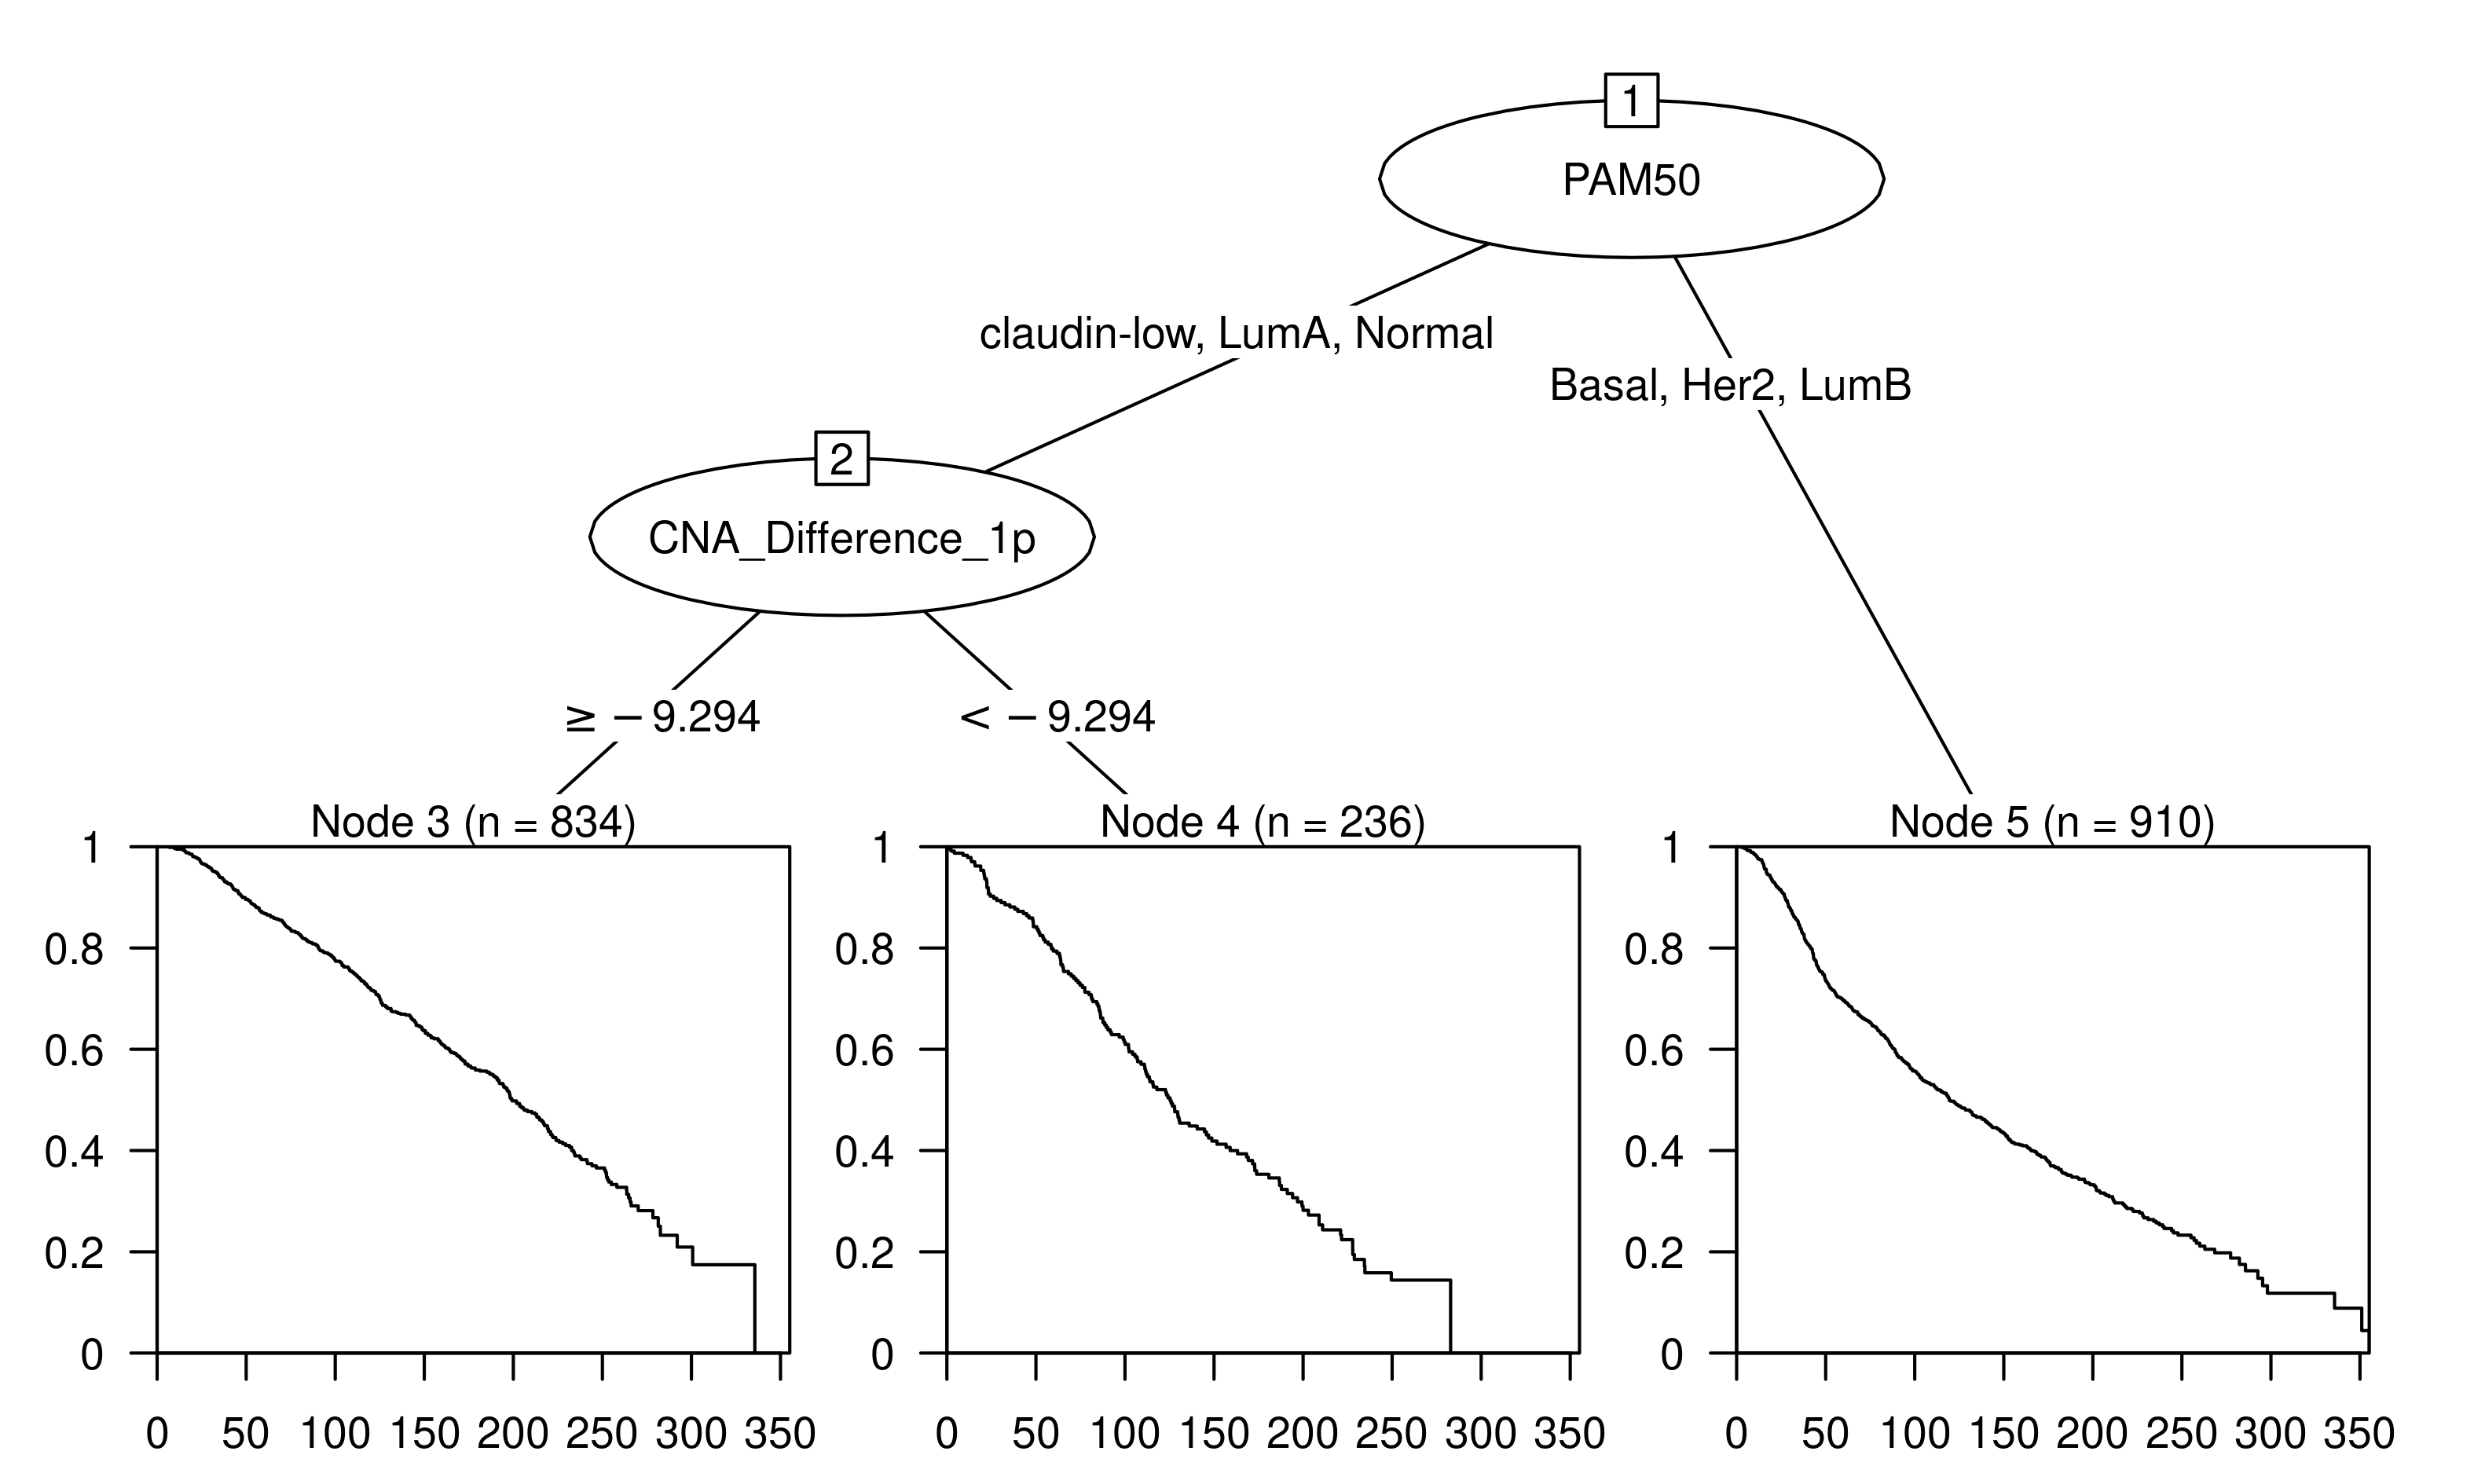
\includegraphics[width=1\textwidth]{../figures/Appendices/Appendix_B/PA_PartyKit_Survival_Burden_OS_PAM50.png}
\end{subfigure}

\vspace{2cm}

\begin{subfigure}{\textwidth}
\subcaption{}
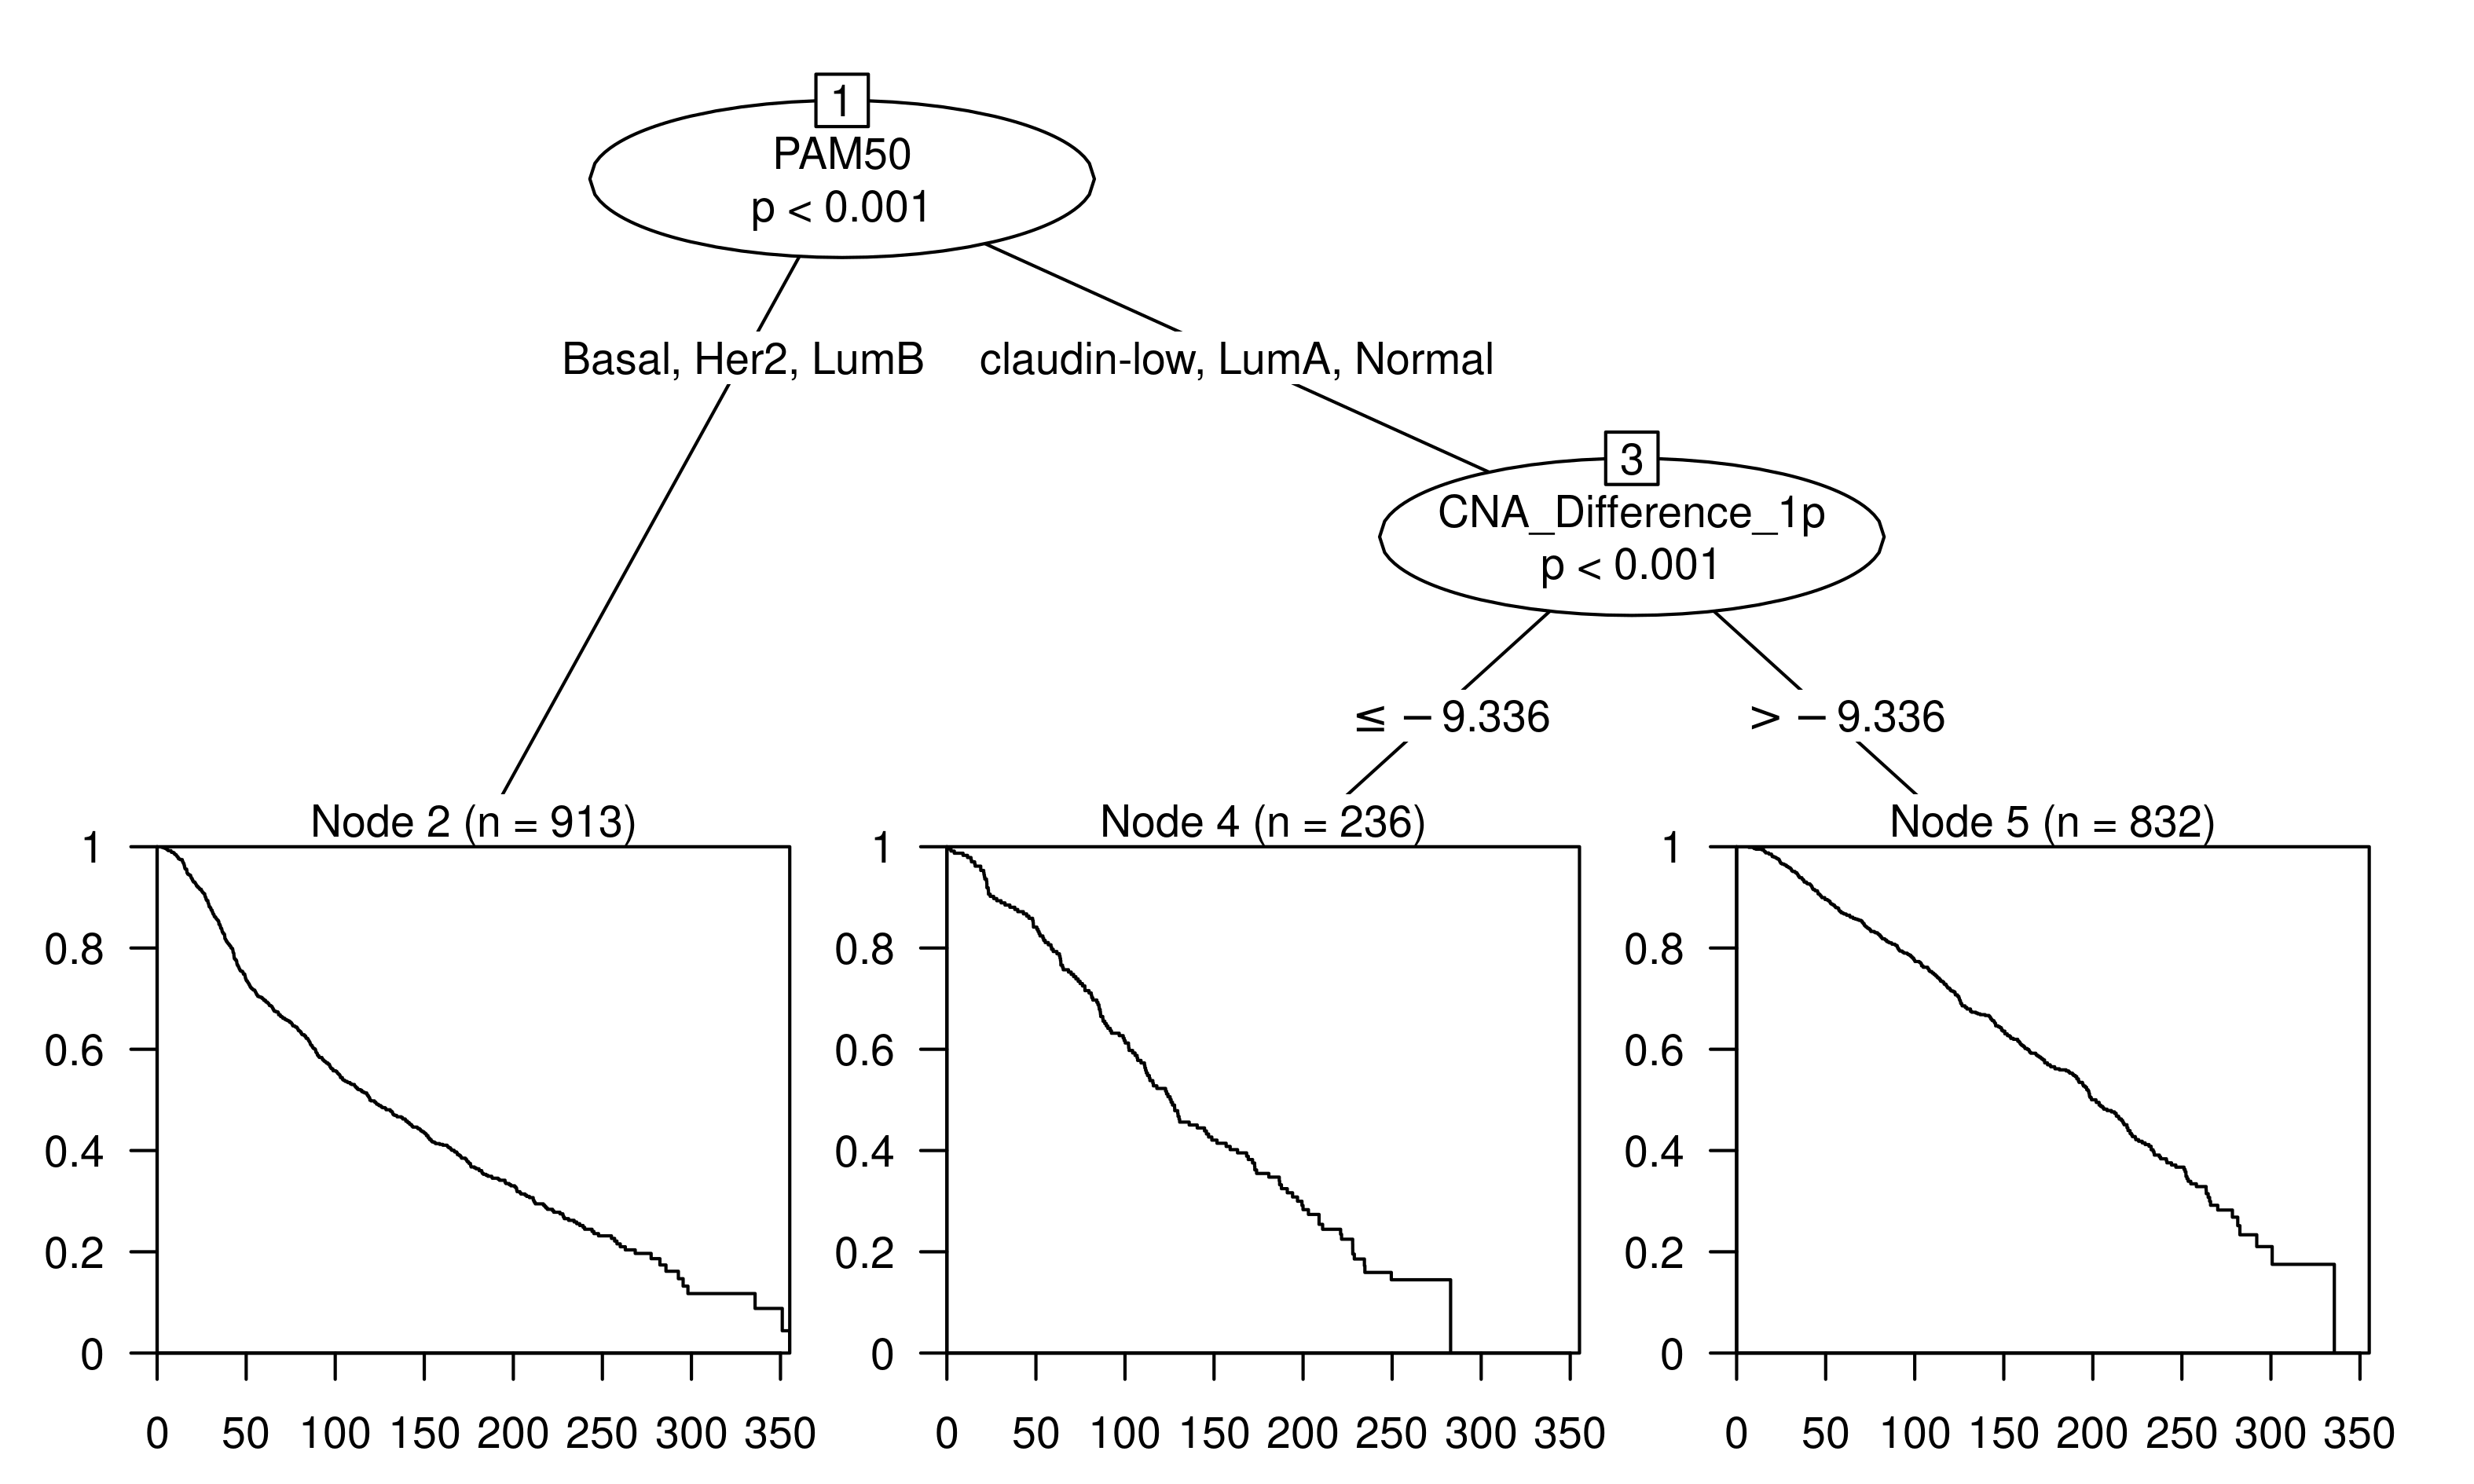
\includegraphics[width=1\textwidth]{../figures/Appendices/Appendix_B/PA_Ctree_Survival_Burden_OS_PAM50.png}
\end{subfigure}

\vspace{0.5cm}

\caption[Recursive partitioning survival trees for overall survival using PAM50 and the 42 chromosome arm CNA Burden metrics as candidate predictors.]{Recursive partitioning survival trees for overall survival using PAM50 and the 42 chromosome arm CNA Burden metrics as candidate predictors. (A) Trees fitted using the rpart algorithm and (B) trees fitted using the ctree algorithm.}
\end{figure}

\begin{figure}[!htb]
\centering

\vspace{0.5cm}

\begin{subfigure}{\textwidth}
\subcaption{}
\includegraphics[width=1\textwidth]{../figures/Appendices/Appendix_B/PA_PartyKit_Survival_Burden_FiveYearOS_PAM50.png}
\end{subfigure}

\vspace{2cm}

\begin{subfigure}{\textwidth}
\subcaption{}
\includegraphics[width=1\textwidth]{../figures/Appendices/Appendix_B/PA_Ctree_Survival_Burden_FiveYearOS_PAM50.png}
\end{subfigure}

\vspace{0.5cm}

\caption[Recursive partitioning survival trees for five-year overall survival using PAM50 and the 42 chromosome arm CNA Burden metrics as candidate predictors.]{Recursive partitioning survival trees for five-year overall survival using PAM50 and the 42 chromosome arm CNA Burden metrics as candidate predictors. (A) Trees fitted using the rpart algorithm and (B) trees fitted using the ctree algorithm.}
\end{figure}

\begin{figure}[!htb]
\centering

\vspace{0.5cm}

\begin{subfigure}{\textwidth}
\subcaption{}
\includegraphics[width=1\textwidth]{../figures/Appendices/Appendix_B/PA_PartyKit_Survival_Burden_TenYearOS_PAM50.png}
\end{subfigure}

\vspace{2cm}

\begin{subfigure}{\textwidth}
\subcaption{}
\includegraphics[width=1\textwidth]{../figures/Appendices/Appendix_B/PA_Ctree_Survival_Burden_TenYearOS_PAM50.png}
\end{subfigure}

\vspace{0.5cm}

\caption[Recursive partitioning survival trees for five-year overall survival using PAM50 and the 42 chromosome arm CNA Burden metrics as candidate predictors.]{Recursive partitioning survival trees for five-year overall survival using PAM50 and the 42 chromosome arm CNA Burden metrics as candidate predictors. (A) Trees fitted using the rpart algorithm and (B) trees fitted using the ctree algorithm.}
\end{figure}

% OS using IntClust and the 42 CNA Score metrics as candidate predictors
\begin{figure}[!htb]
\centering

\vspace{0.5cm}

\begin{subfigure}{\textwidth}
\subcaption{}
\includegraphics[width=1\textwidth]{../figures/Appendices/Appendix_B/PA_PartyKit_Survival_Score_OS_INTCLUST.png}
\end{subfigure}

\vspace{2cm}

\begin{subfigure}{\textwidth}
\subcaption{}
\includegraphics[width=1\textwidth]{../figures/Appendices/Appendix_B/PA_Ctree_Survival_Score_OS_INTCLUST.png}
\end{subfigure}

\vspace{0.5cm}

\caption[Recursive partitioning survival trees for overall survival using Integrative Cluster and the 42 chromosome arm CNA Score metrics as candidate predictors.]{Recursive partitioning survival trees for overall survival using Integrative Cluster and the 42 chromosome arm CNA Score metrics as candidate predictors. (A) Trees fitted using the rpart algorithm and (B) trees fitted using the ctree algorithm.}
\end{figure}

\begin{figure}[!htb]
\centering

\vspace{0.5cm}

\begin{subfigure}{\textwidth}
\subcaption{}
\includegraphics[width=1\textwidth]{../figures/Appendices/Appendix_B/PA_PartyKit_Survival_Score_FiveYearOS_INTCLUST.png}
\end{subfigure}

\vspace{2cm}

\begin{subfigure}{\textwidth}
\subcaption{}
\includegraphics[width=1\textwidth]{../figures/Appendices/Appendix_B/PA_Ctree_Survival_Score_FiveYearOS_INTCLUST.png}
\end{subfigure}

\vspace{0.5cm}

\caption[Recursive partitioning survival trees for five-year overall survival using Integrative Cluster and the 42 chromosome arm CNA Score metrics as candidate predictors.]{Recursive partitioning survival trees for five-year overall survival using Integrative Cluster and the 42 chromosome arm CNA Score metrics as candidate predictors. (A) Trees fitted using the rpart algorithm and (B) trees fitted using the ctree algorithm.}
\end{figure}


\begin{figure}[!htb]
\centering

\vspace{0.5cm}

\begin{subfigure}{\textwidth}
\subcaption{}
\includegraphics[width=1\textwidth]{../figures/Appendices/Appendix_B/PA_PartyKit_Survival_Score_TenYearOS_INTCLUST.png}
\end{subfigure}

\vspace{2cm}

\begin{subfigure}{\textwidth}
\subcaption{}
\includegraphics[width=1\textwidth]{../figures/Appendices/Appendix_B/PA_Ctree_Survival_Score_TenYearOS_INTCLUST.png}
\end{subfigure}

\vspace{0.5cm}

\caption[Recursive partitioning survival trees for five-year overall survival using Integrative Cluster and the 42 chromosome arm CNA Score metrics as candidate predictors.]{Recursive partitioning survival trees for five-year overall survival using  Integrative Cluster and the 42 chromosome arm CNA Score metrics as candidate predictors. (A) Trees fitted using the rpart algorithm and (B) trees fitted using the ctree algorithm.}
\end{figure}

% OS using IntClust and the 42 CNA Burden metrics as candidate predictors
\begin{figure}[!htb]
\centering

\vspace{0.5cm}

\begin{subfigure}{\textwidth}
\subcaption{}
\includegraphics[width=1\textwidth]{../figures/Appendices/Appendix_B/PA_PartyKit_Survival_Burden_OS_INTCLUST.png}
\end{subfigure}

\vspace{2cm}

\begin{subfigure}{\textwidth}
\subcaption{}
\includegraphics[width=1\textwidth]{../figures/Appendices/Appendix_B/PA_Ctree_Survival_Burden_OS_INTCLUST.png}
\end{subfigure}

\vspace{0.5cm}

\caption[Recursive partitioning survival trees for overall survival using Integrative Cluster and the 42 chromosome arm CNA Burden metrics as candidate predictors.]{Recursive partitioning survival trees for overall survival using Integrative Cluster and the 42 chromosome arm CNA Burden metrics as candidate predictors. (A) Trees fitted using the rpart algorithm and (B) trees fitted using the ctree algorithm.}
\end{figure}

\begin{figure}[!htb]
\centering

\vspace{0.5cm}

\begin{subfigure}{\textwidth}
\subcaption{}
\includegraphics[width=1\textwidth]{../figures/Appendices/Appendix_B/PA_PartyKit_Survival_Burden_FiveYearOS_INTCLUST.png}
\end{subfigure}

\vspace{2cm}

\begin{subfigure}{\textwidth}
\subcaption{}
\includegraphics[width=1\textwidth]{../figures/Appendices/Appendix_B/PA_Ctree_Survival_Burden_FiveYearOS_INTCLUST.png}
\end{subfigure}

\vspace{0.5cm}

\caption[Recursive partitioning survival trees for five-year overall survival using Integrative Cluster and the 42 chromosome arm CNA Burden metrics as candidate predictors.]{Recursive partitioning survival trees for five-year overall survival using Integrative Cluster and the 42 chromosome arm CNA Burden metrics as candidate predictors. (A) Trees fitted using the rpart algorithm and (B) trees fitted using the ctree algorithm.}
\end{figure}

\begin{figure}[!htb]
\centering

\vspace{0.5cm}

\begin{subfigure}{\textwidth}
\subcaption{}
\includegraphics[width=1\textwidth]{../figures/Appendices/Appendix_B/PA_PartyKit_Survival_Burden_TenYearOS_INTCLUST.png}
\end{subfigure}

\vspace{2cm}

\begin{subfigure}{\textwidth}
\subcaption{}
\includegraphics[width=1\textwidth]{../figures/Appendices/Appendix_B/PA_Ctree_Survival_Burden_TenYearOS_INTCLUST.png}
\end{subfigure}

\vspace{0.5cm}

\caption[Recursive partitioning survival trees for five-year overall survival using Integrative Cluster and the 42 chromosome arm CNA Burden metrics as candidate predictors.]{Recursive partitioning survival trees for five-year overall survival using  Integrative Cluster and the 42 chromosome arm CNA Burden metrics as candidate predictors. (A) Trees fitted using the rpart algorithm and (B) trees fitted using the ctree algorithm.}
\end{figure}

% OS using PAM50 Subtype, the 42 CNA Burden metrics and a number of clinical variables as candidate predictors
\begin{figure}[!htb]
\centering

\vspace{1cm}

\begin{subfigure}{\textwidth}
\subcaption{}
\includegraphics[width=1\textwidth]{../figures/Appendices/Appendix_B/Clin_PA_PartyKit_Survival_Burden_OS_PAM50.png}
\end{subfigure}

\vspace{2cm}

\begin{subfigure}{\textwidth}
\subcaption{}
\includegraphics[width=1\textwidth]{../figures/Appendices/Appendix_B/Clin_PA_Ctree_Survival_Burden_OS_PAM50.png}
\end{subfigure}

\vspace{1cm}

\caption[Recursive partitioning survival trees for overall survival using PAM50, the 42 CNA Burden metrics and a number of clinical variables as candidate predictors.]{Recursive partitioning survival trees for overall survival using PAM50, the 42 CNA Burden metrics and a number of clinical variables as candidate predictors. (A) Trees fitted using the rpart algorithm and (B) trees fitted using the ctree algorithm.}
\end{figure}

\begin{figure}[!htb]
\centering

\vspace{1cm}

\begin{subfigure}{\textwidth}
\subcaption{}
\includegraphics[width=1\textwidth]{../figures/Appendices/Appendix_B/Clin_PA_PartyKit_Survival_Burden_FiveYearOS_PAM50.png}
\end{subfigure}

\vspace{2cm}

\begin{subfigure}{\textwidth}
\subcaption{}
\includegraphics[width=1\textwidth]{../figures/Appendices/Appendix_B/Clin_PA_Ctree_Survival_Burden_FiveYearOS_PAM50.png}
\end{subfigure}

\vspace{1cm}

\caption[Recursive partitioning survival trees for five-year overall survival using PAM50, the 42 CNA Burden metrics and a number of clinical variables as candidate predictors.]{Recursive partitioning survival trees for five-year overall survival using PAM50, the 42 CNA Burden metrics and a number of clinical variables as candidate predictors. (A) Trees fitted using the rpart algorithm and (B) trees fitted using the ctree algorithm.}
\end{figure}

\begin{figure}[!htb]
\centering

\vspace{1cm}

\begin{subfigure}{\textwidth}
\subcaption{}
\includegraphics[width=1\textwidth]{../figures/Appendices/Appendix_B/Clin_PA_PartyKit_Survival_Burden_TenYearOS_PAM50.png}
\end{subfigure}

\vspace{2cm}

\begin{subfigure}{\textwidth}
\subcaption{}
\includegraphics[width=1\textwidth]{../figures/Appendices/Appendix_B/Clin_PA_Ctree_Survival_Burden_TenYearOS_PAM50.png}
\end{subfigure}

\vspace{1cm}

\caption[Recursive partitioning survival trees for ten-year overall survival using PAM50, the 42 CNA Burden metrics and a number of clinical variables as candidate predictors.]{Recursive partitioning survival trees for ten-year overall survival using PAM50, the 42 CNA Burden metrics and a number of clinical variables as candidate predictors. (A) Trees fitted using the rpart algorithm and (B) trees fitted using the ctree algorithm.}
\end{figure}

% OS using IntClust, the 42 CNA Burden metrics and a number of clinical variables as candidate predictors
\begin{figure}[!htb]
\centering

\vspace{1cm}

\begin{subfigure}{\textwidth}
\subcaption{}
\includegraphics[width=1\textwidth]{../figures/Appendices/Appendix_B/Clin_PA_PartyKit_Survival_Burden_OS_INTCLUST.png}
\end{subfigure}

\vspace{2cm}

\begin{subfigure}{\textwidth}
\subcaption{}
\includegraphics[width=1\textwidth]{../figures/Appendices/Appendix_B/Clin_PA_Ctree_Survival_Burden_OS_INTCLUST.png}
\end{subfigure}

\vspace{1cm}

\caption[Recursive partitioning survival trees for overall survival using INTCLUST, the 42 CNA Burden metrics and a number of clinical variables as candidate predictors.]{Recursive partitioning survival trees for overall survival using INTCLUST, the 42 CNA Burden metrics and a number of clinical variables as candidate predictors. (A) Trees fitted using the rpart algorithm and (B) trees fitted using the ctree algorithm.}
\end{figure}

\begin{figure}[!htb]
\centering

\vspace{1cm}

\begin{subfigure}{\textwidth}
\subcaption{}
\includegraphics[width=1\textwidth]{../figures/Appendices/Appendix_B/Clin_PA_PartyKit_Survival_Burden_FiveYearOS_INTCLUST.png}
\end{subfigure}

\vspace{2cm}

\begin{subfigure}{\textwidth}
\subcaption{}
\includegraphics[width=1\textwidth]{../figures/Appendices/Appendix_B/Clin_PA_Ctree_Survival_Burden_FiveYearOS_INTCLUST.png}
\end{subfigure}

\vspace{1cm}

\caption[Recursive partitioning survival trees for five-year overall survival using INTCLUST, the 42 CNA Burden metrics and a number of clinical variables as candidate predictors.]{Recursive partitioning survival trees for five-year overall survival using INTCLUST, the 42 CNA Burden metrics and a number of clinical variables as candidate predictors. (A) Trees fitted using the rpart algorithm and (B) trees fitted using the ctree algorithm.}
\end{figure}

\begin{figure}[!htb]
\centering

\vspace{1cm}

\begin{subfigure}{\textwidth}
\subcaption{}
\includegraphics[width=1\textwidth]{../figures/Appendices/Appendix_B/Clin_PA_PartyKit_Survival_Burden_TenYearOS_INTCLUST.png}
\end{subfigure}

\vspace{2cm}

\begin{subfigure}{\textwidth}
\subcaption{}
\includegraphics[width=1\textwidth]{../figures/Appendices/Appendix_B/Clin_PA_Ctree_Survival_Burden_TenYearOS_INTCLUST.png}
\end{subfigure}

\vspace{1cm}

\caption[Recursive partitioning survival trees for ten-year overall survival using INTCLUST, the 42 CNA Burden metrics and a number of clinical variables as candidate predictors.]{Recursive partitioning survival trees for ten-year overall survival using INTCLUST, te 42 CNA Burden metrics and a number of clinical variables as candidate predictors. (A) Trees fitted using the rpart algorithm and (B) trees fitted using the ctree algorithm.}
\end{figure}
\FloatBarrier


\section*{Appendix C}
\renewcommand{\thefigure}{C\arabic{figure}}
\renewcommand{\thetable}{C\arabic{table}}
\setcounter{figure}{0}
\setcounter{table}{0}

\phantomsection
\addcontentsline{toc}{section}{Appendix C}

\markboth{\MakeUppercase{APPENDIX C}}{\MakeUppercase{APPENDIX C}}
\captionsetup[subfigure]{font={normalfont,small}, skip=1pt, margin=-0.0cm, singlelinecheck=false}

Appendix C contains lists of genes measured on the Oncotype DX assay, MammaPrint assay, Prosigna (PAM50) assay and BCI assay. 

% Oncotype DX
{\normalsize
\begin{table}[!htb]
\caption{The 21 genes included in the Oncotype DX assay \citep{pmid15591335}.}
\center
\begin{tabular}{|c|c|}
\hline
\multicolumn{1}{|c|}{\textbf{Gene Symbol}} & \textbf{Oncotype DX Category} \\ 
\hline
ACTB & Reference gene  \\
GAPDH & Reference gene \\
GUSB & Reference gene \\
RPLPO & Reference gene \\ 
TFRC & Reference gene \\ 
\hline
MKI67 & Proliferation-related gene  \\
AURKA & Proliferation-related gene \\
BIRC5 & Proliferation-related gene \\
CCNB1 & Proliferation-related gene \\ 
MYBL2 & Proliferation-related gene \\ 
\hline 
MMP11 & Metastasis-related gene \\
CTSL2 & Metastasis-related gene \\ 
\hline 
GRB7 & HER2-related gene \\
ERBB2 & HER2-related gene \\  
\hline
ESR1 &  Hormone-related gene  \\
PGR & Hormone-related gene \\
SCUBE2 & Hormone-related gene \\
BCL2 & Hormone-related gene \\ 
GSTM1 & Hormone-related gene \\ 
BAG1 & Hormone-related gene \\
CD68 & Hormone-related gene \\
\hline
\end{tabular}
\label{Oncotype_DX_GS}
\end{table}
}

% MammaPrint
{\footnotesize
\begin{longtable}[!htb]{|c|c|}
\caption{The 70 genes included in the MammaPrint assay \citep{pmid11823860, pmid21151591}.}
\label{MammaPrint_GS} \\
\hline
\textbf{Gene Symbol} & \textbf{MammaPrint Category} \\ 
\hline
BBC3 & Evading apoptosis \\
\hline
EGLN1 & Evading apoptosis and sustained angiogenesis \\
\hline
FLT1 & Evading apoptosis and sustained angiogenesis\\
\hline
HRASLS & Evading apoptosis \\
\hline
STK32B & Evading apoptosis \\
\hline
TGFB3 & Insensitivity to anti-growth signals and self-sufficiency in growth signals \\
\hline
RASSF7 & Insensitivity to anti-growth signals \\
\hline
DCK & Insensitivity to anti-growth signals \\
\hline
MELK & Insensitivity to anti-growth signals \\
\hline
EXT1 & Insensitivity to anti-growth signals \\
\hline 
ESM1 & Self-sufficiency in growth signals \\
\hline
IGFBP5 & Self-sufficiency in growth signals \\ 
\hline
FGF18 & Self-sufficiency in growth signals and sustained angiogenesis \\ 
\hline
SCUBE2 & Self-sufficiency in growth signals \\ 
\hline
WISP1 & Self-sufficiency in growth signals \\ 
\hline
GNAZ & Self-sufficiency in growth signals \\ 
\hline
EBF4 & Self-sufficiency in growth signals \\ 
\hline
MTDH & Self-sufficiency in growth signals \\ 
\hline
PITRM1 & Self-sufficiency in growth signals \\ 
\hline
QSCN6L1 (QSOX1) & Self-sufficiency in growth signals \\ 
\hline 
CCNE2 & Limitless replicative potential	\\
\hline
ECT2 & Limitless replicative potential \\  
\hline
CENPA & Limitless replicative potential \\  
\hline
LIN9 & Limitless replicative potential \\  
\hline
KNTC2 (NDC80) & Limitless replicative potential \\ 
\hline 
MCM6 & Limitless replicative potential \\  
\hline
NUSAP1 & Limitless replicative potential \\  
\hline
ORC6L & Limitless replicative potential \\  
\hline
TSPYL5 & Limitless replicative potential \\  
\hline
RUNDC1 & Limitless replicative potential \\  
\hline
PRC1 & Limitless replicative potential \\  
\hline
RFC4 & Limitless replicative potential \\  
\hline
RECQL5 & Limitless replicative potential \\ 
\hline
CDCA7 & Limitless replicative potential \\ 
\hline
DTL & Limitless replicative potential \\ 
\hline
COL4A2 & Tissue invasion and metastasis and sustained angiogenesis \\
\hline
GPR180 & Tissue invasion and metastasis and sustained angiogenesis \\
\hline
MMP9 & Tissue invasion and metastasis and sustained angiogenesis\\
\hline
GPR126 & Tissue invasion and metastasis \\
\hline
RTN4RL1 & Tissue invasion and metastasis \\
\hline
CDC42BPA & Tissue invasion and metastasis \\
\hline
DIAPH3 & Tissue invasion and metastasis \\
\hline
PALM2 & Tissue invasion and metastasis \\
\hline
ALDH4A1 & Sustained angiogenesis \\
\hline
AYTL2 (LPCAT2) & Sustained angiogenesis \\
\hline
OXCT1 & Sustained angiogenesis \\
\hline
PECI & Sustained angiogenesis \\
\hline
GMPS (LOC728564) & Sustained angiogenesis \\
\hline
GSTM3 & Sustained angiogenesis \\
\hline
SLC2A3 & Sustained angiogenesis \\
\hline
LOC100288906 & Unknown function \\
\hline
C9orf30 & Unknown function \\
\hline
C20orf46 & Unknown function \\
\hline
ZNF533 & Unknown function \\
\hline
C16orf61 & Unknown function \\
\hline
SERF1A & Unknown function \\
\hline
LOC730018 & Unknown function \\
\hline
LOC100131053 & Unknown function \\
\hline
AA555029\_RC & Unknown function \\
\hline
LGP2 (DHX58) & Miscellaneous \\
\hline
NMU & Miscellaneous \\
\hline
UCHL5 & Miscellaneous \\
\hline
JHDM1D & Miscellaneous \\
\hline
AP2B1 & Miscellaneous \\
\hline
MS4A7 & Miscellaneous \\
\hline
RAB6B & Miscellaneous \\
\hline
\end{longtable}
}

% Progsigna (PAM50)
\begin{table}[!htb]
  \caption{The 58 genes included in the Prosigna assay \citep{DUFFY2017284}}
  \centering
  \begin{tabular}{|c|}
  \hline
    \textbf{Gene Symbol} \\ 
\hline
ACTB \\
\hline
GUSB \\ 
\hline
MRPL19 \\
\hline
PSMC4 \\ 
\hline
PUM1 \\
\hline
RPLP0  \\
\hline
SF3A1 \\
\hline
TFRC \\
\hline
ACTR3B \\
\hline
ANLN \\
\hline
BAG1 \\
\hline
BCL2 \\
\hline 
BIRC5 \\ 
\hline
BLVRA \\
\hline
CCNB1 \\
\hline
CCNE1 \\
\hline
CDC20 \\ 
\hline
CDC6 \\ 
\hline
CDCA1 \\ 
\hline
CDH3 \\ 
\hline
CENPF \\ 
\hline
CEP55 \\
\hline
CXXC5 \\
\hline
EGFR \\
\hline 
ERBB2 \\
\hline 
ESR1 \\
\hline 
EXO1 \\ 
\hline
FGFR4 \\ 
\hline
FOXA1 \\ 
\hline
  \end{tabular}
  \hspace{1em}
  \begin{tabular}{|c|}
  \hline
   \textbf{Gene Symbol} \\ 
\hline
FOXC1 \\ 
\hline
GPR160 \\
\hline 
GRB7 \\ 
\hline
KIF2C \\ 
\hline
KNTC2  \\
\hline
KRT14 \\ 
\hline 
KRT17 \\ 
\hline 
KRT5 \\ 
\hline 
MAPT \\ 
\hline 
MDM2 \\ 
\hline 
MELK \\
\hline 
MIA \\
\hline
MKI67 \\ 
\hline 
MLPH \\ 
\hline 
MMP11 \\ 
\hline 
MYBL2 \\ 
\hline 
MYC \\ 
\hline 
NAT1 \\
\hline 
ORC6L \\
\hline
PGR \\ 
\hline 
PHGDH \\
\hline
PTTG1 \\
\hline
RRM2 \\
\hline
SFRP1 \\
\hline
SLC39A6 \\
\hline
TMEM45B \\ 
\hline
TYMS \\
\hline 
UBE2C \\ 
\hline
UBE2T \\
\hline
  \end{tabular}
\end{table}

% Breast Cancer Index 
{\normalsize
\begin{table}[!htb]
\caption{The 11 genes included in the Breast Cancer Index assay \citep{pmid21559019}.}
\center
\begin{tabular}{|c|c|}
\hline
\multicolumn{1}{|c|}{\textbf{Gene Symbol}} & \textbf{BCI Category} \\ 
\hline
ACTB & Reference gene  \\
HMBS & Reference gene \\
SDHA & Reference gene \\
UBC & Reference gene \\ 
\hline
HOXB13 & H:I index gene \\
IL17BR & H:I index gene \\
\hline 
BUB1B & Molecular Grade Index gene \\
CENPA & Molecular Grade Index gene \\
NEK2 & Molecular Grade Index gene \\
RACGAP1 & Molecular Grade Index gene \\
RRM2 & Molecular Grade Index gene \\
\hline
\end{tabular}
\label{BCI_GS}
\end{table}
}
\FloatBarrier
\section*{Appendix D}
\renewcommand{\thefigure}{D\arabic{figure}}
\renewcommand{\thetable}{D\arabic{table}}
\setcounter{figure}{0}
\setcounter{table}{0}

\phantomsection
\addcontentsline{toc}{section}{Appendix D}

\markboth{\MakeUppercase{APPENDIX D}}{\MakeUppercase{APPENDIX D}}

Appendix D contains a list of genes that are present in the METABRIC CNA and gene expression data utilised in this thesis but missing from the IntClust gene list. 

% IntClust Genes 
% latex table generated in R 4.3.1 by xtable 1.8-4 package
% Mon Nov 20 14:36:07 2023

\begin{xltabular}[!htb]{\textwidth}{|c|c|X|}
\caption{Genes present in our analysis but missing from the IntClust gene set \citep{pmid22522925}.} \label{tab:long} \\

\hline \multicolumn{1}{|c|}{\textbf{ProbeID}} & \multicolumn{1}{c|}{\textbf{Gene}} & \multicolumn{1}{c|}{\textbf{Gene Description}} \\ \hline 
\endfirsthead

\multicolumn{3}{c}%
{\tablename\ \thetable{} -- continued from previous page} \\
\hline \multicolumn{1}{|c|}{\textbf{ProbeID}} & \multicolumn{1}{c|}{\textbf{Gene}} & \multicolumn{1}{c|}{\textbf{Gene Description}} \\ \hline 
\endhead

\hline \multicolumn{3}{|r|}{{Continued on next page}} \\ \hline
\endfoot

\hline
\endlastfoot

  ILMN\_2044617 & MTERFD1 & MTERF domain containing 1 \\ 
  ILMN\_1679867 & LOC642255 & Heat shock transcription factor 1 \\ 
  ILMN\_1720819 & LOC653566 & Signal peptidase complex subunit 2 homolog (S. cerevisiae) \\ 
  ILMN\_1783469 & LOC642197 & Family with sequence similarity 82, member B \\ 
  ILMN\_1675406 & PPAPDC1B & Phosphatidic acid phosphatase type 2 domain containing 1B \\ 
  ILMN\_1685774 & LOC647340 & ATP synthase, H+ transporting, mitochondrial F1 complex, gamma polypeptide 1 \\ 
  ILMN\_1665423 & ZFP91 & Zinc finger protein 91 homolog (mouse) \\ 
  ILMN\_1764323 & LOC124512 & Chromosome 17 open reading frame 95 \\ 
  ILMN\_1763955 & LOC653119 & Block of proliferation 1 \\ 
  ILMN\_1665483 & KIAA0020 & KIAA0020 \\ 
  ILMN\_1651899 & LOC653314 &  \\ 
  ILMN\_1780141 & TMEM66 & Transmembrane protein 66 \\ 
  ILMN\_1769118 & 38595 & Septin 9 \\ 
  ILMN\_1699253 & LOC729317 & Voltage-dependent anion channel 2 \\ 
  ILMN\_1693862 & MGC70857 & Chromosome 8 open reading frame 82 \\ 
  ILMN\_1784436 & KIAA1688 & KIAA1688 protein \\ 
  ILMN\_1796235 & CIRH1A & Cirrhosis, autosomal recessive 1A (cirhin) \\ 
  ILMN\_1785660 & SRPR & Signal recognition particle receptor (docking protein) \\ 
  ILMN\_1687921 & LOC339123 & Jumonji domain containing 8 \\ 
  ILMN\_2402930 & LOC440926 & H3 histone, family 3A \\ 
  ILMN\_1746706 & LOC653103 & Ankyrin repeat domain 11 \\ 
  ILMN\_2112599 & C16orf80 & Chromosome 16 open reading frame 80 \\ 
  ILMN\_1879344 & HS.571404 & Calpain 1, (mu/I) large subunit \\ 
  ILMN\_1675542 & LOC729148 & Nuclear undecaprenyl pyrophosphate synthase 1 homolog (S. cerevisiae) \\ 
  ILMN\_1740351 & KIAA0174 & KIAA0174 \\ 
  ILMN\_1814812 & LOC650546 & Ubiquitin specific peptidase 32 \\ 
  ILMN\_1790162 & LOC441155 & Zinc finger CCCH-type containing 11A \\ 
  ILMN\_2059211 & KIAA0195 & KIAA0195 \\ 
  ILMN\_2172269 & TMEM183B & Transmembrane protein 183B \\ 
  ILMN\_1655403 & LOC730083 & Exoribonuclease 2 \\ 
  ILMN\_1763404 & LOC653226 & Homo sapiens clone 24452 mRNA sequence. \\ 
  ILMN\_1700461 & AARSD1 & Alanyl-tRNA synthetase domain containing 1 \\ 
  ILMN\_1759991 & MGC3731 & Nucleolar protein 12 \\ 
  ILMN\_1733757 & LOC374395 & Transmembrane protein 179B \\ 
  ILMN\_1753790 & ZNF259 & Zinc finger protein 259 \\ 
  ILMN\_1746206 & AZI1 & 5-azacytidine induced 1 \\ 
  ILMN\_1763663 & FLJ20718 & HEAT repeat containing 3 \\ 
  ILMN\_1655819 & LOC728919 & Anaphase promoting complex subunit 11 \\ 
  ILMN\_1686401 & LOC728739 & Programmed cell death 2 \\ 
  ILMN\_1669424 & LOC646531 & Y box binding protein 1 \\ 
  ILMN\_2179726 & LOC90835 & Chromosome 16 open reading frame 93 \\ 

   \hline
\end{xltabular}

\section*{Appendix E}
\renewcommand{\thefigure}{E\arabic{figure}}
\renewcommand{\thetable}{E\arabic{table}}
\setcounter{figure}{0}
\setcounter{table}{0}

\phantomsection
\addcontentsline{toc}{section}{Appendix E}

\markboth{\MakeUppercase{APPENDIX E}}{\MakeUppercase{APPENDIX E}}

Appendix E contains (1) the results obtained for the univariate Allele-Independent Intercept Model and Allele-Independent Non-Intercept Model fitted using the \texttt{MCMCglmm()} function (2) the results obtained for the univariate Allele-Dependent Intercept Model and Allele-Dependent Non-Intercept Model fitted using the \texttt{MCMCglmm()} function and (3) the results obtained for the multivariate Allele-Dependent Intercept Model and Allele-Dependent Non-Intercept Model fitted using the \texttt{MCMCglmm()} function.

\begin{table}[!htb]
    \caption[Univariate Allele-Independent Intercept Model parameter estimates fitted using \texttt{MCMCglmm()}.]{Univariate Allele-Independent Intercept Model parameter estimates fitted using \texttt{MCMCglmm()}. In (A) neutral lengths are recorded as length 0 and in (B) neutral lengths are retained as greater than 0.}
    %\label{tbl:lm_uni_1_model}
     \begin{subtable}[t]{.49\textwidth}
      \centering
      \includegraphics[width = 1\textwidth]{../tables/Chapter_5/Univariate_MCMC_7_AI_Model.png}
    \end{subtable}%
    \hspace{0.5cm}
     \begin{subtable}[t]{.49\textwidth}
      \centering
         \includegraphics[width = 1\textwidth]{../tables/Chapter_5/Univariate_MCMC_7_Neut_AI_Model.png}
    \end{subtable} 
\end{table}

\begin{table}[!htb]
    \caption[Univariate Allele-Independent Intercept Model parameter estimates fitted using \texttt{MCMCglmm()}.]{Univariate Allele-Independent Intercept Model parameter estimates fitted using \texttt{MCMCglmm()}. In (A) neutral lengths are recorded as length 0 and in (B) neutral lengths are retained as greater than 0.}
    %\label{tbl:lm_uni_1_pred}
     \begin{subtable}[t]{.49\textwidth}
      \centering
      \includegraphics[width = 1\textwidth]{../tables/Chapter_5/Univariate_MCMC_7_AI_Pred.png}
    \end{subtable}%
    \hspace{0.5cm}
     \begin{subtable}[t]{.49\textwidth}
      \centering
         \includegraphics[width = 1\textwidth]{../tables/Chapter_5/Univariate_MCMC_7_Neut_AI_Pred.png}
    \end{subtable} 
\end{table}

\begin{figure}[!htb]
\vspace{0.5cm}
     \begin{subfigure}[t]{.49\textwidth}
      \centering
      \includegraphics[width = 1\textwidth]{../figures/Chapter_5/Univariate_MCMC_7_AI_Interval.png}
    \end{subfigure}%
     \begin{subfigure}[t]{.49\textwidth}
      \centering
       \includegraphics[width = 1\textwidth]{../figures/Chapter_5/Univariate_MCMC_7_Neut_AI_Interval.png}
    \end{subfigure} 
     \caption[Interval plot of univariate Allele-Independent Intercept Model parameter estimates fitted using \texttt{MCMCglmm()}.]{Interval plot of univariate Allele-Independent Intercept Model parameter estimates fitted using \texttt{MCMCglmm()}. In (A) neutral lengths are recorded as length 0 and in (B) neutral lengths are retained as greater than 0.}
    % \label{fig:lm_uni_1_int}
\end{figure}

\begin{table}[!htb]
    \caption[Univariate Allele-Independent Non-Intercept Model parameter estimates fitted using \texttt{MCMCglmm()}.]{Univariate Allele-Independent Non-Intercept Model parameter estimates fitted using \texttt{MCMCglmm()}. In (A) neutral lengths are recorded as length 0 and in (B) neutral lengths are retained as greater than 0.}
    %\label{tbl:lm_uni_2_model}
     \begin{subtable}[t]{.49\textwidth}
      \centering
      \includegraphics[width = 1\textwidth]{../tables/Chapter_5/Univariate_MCMC_6_AI_Model.png}
    \end{subtable}%
    \hspace{0.5cm}
     \begin{subtable}[t]{.49\textwidth}
      \centering
         \includegraphics[width = 1\textwidth]{../tables/Chapter_5/Univariate_MCMC_6_Neut_AI_Model.png}
    \end{subtable} 
\end{table}

\begin{table}[!htb]
    \caption[Univariate Allele-Independent Non-Intercept Model parameter estimates fitted using \texttt{MCMCglmm()}.]{Univariate Allele-Independent Non-Intercept Model parameter estimates fitted using \texttt{MCMCglmm()}. In (A) neutral lengths are recorded as length 0 and in (B) neutral lengths are retained as greater than 0.}
    %\label{tbl:lm_uni_2_pred}
     \begin{subtable}[t]{.49\textwidth}
      \centering
      \includegraphics[width = 1\textwidth]{../tables/Chapter_5/Univariate_MCMC_6_AI_Pred.png}
    \end{subtable}%
    \hspace{0.5cm}
     \begin{subtable}[t]{.49\textwidth}
      \centering
         \includegraphics[width = 1\textwidth]{../tables/Chapter_5/Univariate_MCMC_6_Neut_AI_Pred.png}
    \end{subtable} 
\end{table}

\begin{figure}[!htb]
\vspace{0.5cm}
     \begin{subfigure}[t]{.49\textwidth}
      \centering
      \includegraphics[width = 1\textwidth]{../figures/Chapter_5/Univariate_MCMC_6_AI_Interval.png}
    \end{subfigure}%
     \begin{subfigure}[t]{.49\textwidth}
      \centering
       \includegraphics[width = 1\textwidth]{../figures/Chapter_5/Univariate_MCMC_6_Neut_AI_Interval.png}
    \end{subfigure} 
     \caption[Interval plot of univariate Allele-Independent Non-Intercept Model parameter estimates fitted using \texttt{MCMCglmm()}.]{Interval plot of univariate Allele-Independent Non-Intercept Model parameter estimates fitted using \texttt{MCMCglmm()}. In (A) neutral lengths are recorded as length 0 and in (B) neutral lengths are retained as greater than 0.}
     %\label{fig:lm_uni_2_int}
\end{figure}

\begin{table}[!htb]
    \caption[Multivariate Allele-Independent Intercept Model parameter estimates fitted using \texttt{MCMCglmm()}.]{Multivariate Allele-Independent Intercept Model parameter estimates fitted using \texttt{MCMCglmm()}. In (A) neutral lengths are recorded as length 0 and in (B) neutral lengths are retained as greater than 0.}
    %\label{tbl:lm_multi_1_model}
     \begin{subtable}[t]{.49\textwidth}
      \centering
      \includegraphics[width = 1\textwidth]{../tables/Chapter_5/Multivariate_MCMC_7_AI_Model.png}
    \end{subtable}%
    \hspace{0.5cm}
     \begin{subtable}[t]{.49\textwidth}
      \centering
         \includegraphics[width = 1\textwidth]{../tables/Chapter_5/Multivariate_MCMC_7_Neut_AI_Model.png}
    \end{subtable} 
\end{table}

\begin{table}[!htb]
    \caption[Multivariate Allele-Independent Intercept Model parameter estimates fitted using \texttt{MCMCglmm()}.]{Multivariate Allele-Independent Intercept Model parameter estimates fitted using \texttt{MCMCglmm()}. In (A) neutral lengths are recorded as length 0 and in (B) neutral lengths are retained as greater than 0.}
    %\label{tbl:lm_multi_1_pred}
     \begin{subtable}[t]{.49\textwidth}
      \centering
      \includegraphics[width = 1\textwidth]{../tables/Chapter_5/Multivariate_MCMC_7_AI_Pred.png}
    \end{subtable}%
    \hspace{0.5cm}
     \begin{subtable}[t]{.49\textwidth}
      \centering
         \includegraphics[width = 1\textwidth]{../tables/Chapter_5/Multivariate_MCMC_7_Neut_AI_Pred.png}
    \end{subtable} 
\end{table}

\begin{figure}[!htb]
\vspace{0.5cm}
     \begin{subfigure}[t]{.49\textwidth}
      \centering
      \includegraphics[width = 1\textwidth]{../figures/Chapter_5/Multivariate_MCMC_7_AI_Interval.png}
    \end{subfigure}%
     \begin{subfigure}[t]{.49\textwidth}
      \centering
       \includegraphics[width = 1\textwidth]{../figures/Chapter_5/Multivariate_MCMC_7_Neut_AI_Interval.png}
    \end{subfigure} 
     \caption[Interval plot of multivariate Allele-Independent Intercept Model parameter estimates fitted using \texttt{MCMCglmm()}.]{Interval plot of multivariate Allele-Independent Intercept Model parameter estimates fitted using \texttt{MCMCglmm()}. In (A) neutral lengths are recorded as length 0 and in (B) neutral lengths are retained as greater than 0.}
     %\label{fig:lm_multi_1_int}
\end{figure}

\begin{table}[!htb]
    \caption[Multivariate Allele-Independent Non-Intercept Model parameter estimates fitted using \texttt{MCMCglmm()}.]{Multivariate Allele-Independent Non-Intercept Model parameter estimates fitted using \texttt{MCMCglmm()}. In (A) neutral lengths are recorded as length 0 and in (B) neutral lengths are retained as greater than 0.}
   % \label{tbl:lm_multi_2_model}
     \begin{subtable}[t]{.49\textwidth}
      \centering
      \includegraphics[width = 1\textwidth]{../tables/Chapter_5/Multivariate_MCMC_6_AI_Model.png}
    \end{subtable}%
    \hspace{0.5cm}
     \begin{subtable}[t]{.49\textwidth}
      \centering
         \includegraphics[width = 1\textwidth]{../tables/Chapter_5/Multivariate_MCMC_6_Neut_AI_Model.png}
    \end{subtable} 
\end{table}

\begin{table}[!htb]
    \caption[Multivariate Allele-Independent Non-Intercept Model parameter estimates fitted using \texttt{MCMCglmm()}.]{Multivariate Allele-Independent Non-Intercept Model parameter estimates fitted using \texttt{MCMCglmm()}. In (A) neutral lengths are recorded as length 0 and in (B) neutral lengths are retained as greater than 0.}
    %\label{tbl:lm_multi_2_pred}
     \begin{subtable}[t]{.49\textwidth}
      \centering
      \includegraphics[width = 1\textwidth]{../tables/Chapter_5/Multivariate_MCMC_6_AI_Pred.png}
    \end{subtable}%
    \hspace{0.5cm}
     \begin{subtable}[t]{.49\textwidth}
      \centering
         \includegraphics[width = 1\textwidth]{../tables/Chapter_5/Multivariate_MCMC_6_Neut_AI_Pred.png}
    \end{subtable} 
\end{table}

\begin{figure}[!htb]
\vspace{0.5cm}
     \begin{subfigure}[t]{.49\textwidth}
      \centering
      \includegraphics[width = 1\textwidth]{../figures/Chapter_5/Multivariate_MCMC_6_AI_Interval.png}
    \end{subfigure}%
     \begin{subfigure}[t]{.49\textwidth}
      \centering
       \includegraphics[width = 1\textwidth]{../figures/Chapter_5/Multivariate_MCMC_6_Neut_AI_Interval.png}
    \end{subfigure} 
     \caption[Interval plot of multivariate Allele-Independent Non-Intercept Model parameter estimates fitted using \texttt{MCMCglmm()}.]{Interval plot of multivariate Allele-Independent Non-Intercept Model parameter estimates fitted using \texttt{MCMCglmm()}. In (A) neutral lengths are recorded as length 0 and in (B) neutral lengths are retained as greater than 0.}
     %\label{fig:lm_multi_2_int}
\end{figure}

\begin{table}[!htb]
\centering
\caption[Univariate Allele-Dependent Intercept Model parameter estimates and confidence intervals fitted using \texttt{MCMCglmm()}.]{Univariate Allele-Dependent Intercept Model parameter estimates and confidence intervals fitted using \texttt{MCMCglmm()}, where neutral lengths are recorded as length 0.}
      
\includegraphics[width = 1\textwidth]{../tables/Chapter_5/Univariate_MCMC_7_AD_Model_Pred.png}
%\label{tab:lm_uni_AD_modpred}
\end{table}

\begin{figure}[!htb]
\vspace{0.5cm}
     
\centering
\includegraphics[width = 0.8\textwidth]{../figures/Chapter_5/Univariate_MCMC_7_AD_Interval.png}
 
\caption[Interval plot of univariate Allele-Dependent Intercept Model parameter estimates fitted using \texttt{MCMCglmm()}.]{Interval plot of univariate Allele-Dependent Intercept Model parameter estimates fitted using \texttt{MCMCglmm()}, where neutral lengths are recorded as length 0.}
%\label{fig:lm_uni_AD_modpred}
\end{figure}

\begin{table}[!htb]
\centering
\caption[Univariate Allele-Dependent Non-Intercept Model parameter estimates and confidence intervals, fitted using \texttt{MCMCglmm()}.]{Univariate Allele-Dependent Non-Intercept Model parameter estimates and confidence intervals fitted using \texttt{MCMCglmm()}, where neutral lengths are recorded as length 0.}
      
\includegraphics[width = 1\textwidth]{../tables/Chapter_5/Univariate_MCMC_6_AD_Model_Pred.png}
%\label{tab:lm_uni_AD_modpred_6}
\end{table}

\begin{figure}[!htb]
\vspace{0.5cm}
     
\centering
\includegraphics[width = 0.8\textwidth]{../figures/Chapter_5/Univariate_MCMC_6_AD_Interval.png}
 
\caption[Interval plot of univariate Allele-Dependent Non-Intercept Model parameter estimates fitted using \texttt{MCMCglmm()}.]{Interval plot of univariate Allele-Dependent Non-Intercept Model parameter estimates fitted using \texttt{MCMCglmm()}, where neutral lengths are recorded as length 0.}
%\label{fig:lm_uni_AD_modpred_6}
\end{figure}

\begin{table}[!htb]
\centering
\caption[Multivariate Allele-Dependent Intercept Model parameter estimates and confidence intervals fitted using \texttt{MCMCglmm()}.]{Multivariate Allele-Dependent Intercept Model parameter estimates and confidence intervals fitted using \texttt{MCMCglmm()}, where neutral lengths are recorded as length 0.}
      
\includegraphics[width = 1\textwidth]{../tables/Chapter_5/Multivariate_MCMC_7_AD_Model_Pred.png}
%\label{tab:lm_multi_AD_modpred}
\end{table}

\begin{figure}[!htb]
\vspace{0.5cm}
     
\centering
\includegraphics[width = 0.8\textwidth]{../figures/Chapter_5/Multivariate_MCMC_7_AD_Interval.png}
 
\caption[Interval plot of multivariate Allele-Dependent Intercept Model parameter estimates fitted using \texttt{MCMCglmm()}.]{Interval plot of multivariate Allele-Dependent Intercept Model parameter estimates fitted using \texttt{MCMCglmm()}, where neutral lengths are recorded as length 0.}
%\label{fig:lm_multi_AD_modpred}
\end{figure}

\begin{table}[!htb]
\centering
\caption[Multivariate Allele-Dependent Non-Intercept Model parameter estimates and confidence intervals fitted using \texttt{MCMCglmm()}.]{Multivariate Allele-Dependent Non-Intercept Model parameter estimates and confidence intervals fitted using \texttt{MCMCglmm()}, where neutral lengths are recorded as length 0.}
      
\includegraphics[width = 1\textwidth]{../tables/Chapter_5/Multivariate_MCMC_6_AD_Model_Pred.png}
%\label{tab:lm_multi_AD_modpred_6}
\end{table}

\begin{figure}[!htb]
\vspace{0.5cm}
     
\centering
\includegraphics[width = 0.8\textwidth]{../figures/Chapter_5/Multivariate_MCMC_6_AD_Interval.png}
 
\caption[Interval plot of multivariate Allele-Dependent Non-Intercept Model parameter estimates fitted using \texttt{MCMCglmm()}.]{Interval plot of multivariate Allele-Dependent Non-Intercept Model parameter estimates fitted using \texttt{MCMCglmm()}, where neutral lengths are recorded as length 0.}
% \label{fig:lm_multi_modpred_6}
\end{figure}
\FloatBarrier

\section*{Appendix F}
\renewcommand{\thefigure}{F\arabic{figure}}
\renewcommand{\thetable}{F\arabic{table}}
\setcounter{figure}{0}
\setcounter{table}{0}

\phantomsection
\addcontentsline{toc}{section}{Appendix F}

\markboth{\MakeUppercase{APPENDIX F}}{\MakeUppercase{APPENDIX F}}

Appendix F contains allele-specific heatmaps produced for chromosome 18q and 11p and a plot of the frequency of changepoints in genes across chromosome 18q.

\vfill
\begin{figure}[!htb]
\centering
\includegraphics[width = 1\textwidth]{../figures/Chapter_6/Heatmap_Chr18q_Genes_Major.png}
\caption[Heatmap of CNAs across the Major Allele of Chromosome 18q]{Heatmap of CNAs across the Major Allele of Chromosome 18q. The heatmap depicts the CNA state for each gene across Chromosome 18q, partitioning the patients into the nodes corresponding to Figure \ref{fig:INTCLUST_PA_CNA_Burden_DSS}. NAs, depicting multiple states, are coloured in black.}
\label{fig:heatmap_Major_18q}
\end{figure}
\vfill 

\begin{figure}[!htb]
\centering
\includegraphics[width = 1\textwidth]{../figures/Chapter_6/Heatmap_Chr18q_Genes_Minor.png}
\caption[Heatmap of CNAs across the Minor Allele of Chromosome 18q]{Heatmap of CNAs across the Minor Allele of Chromosome 18q. The heatmap depicts the CNA state for each gene across Chromosome 18q, partitioning the patients into the nodes corresponding to Figure \ref{fig:INTCLUST_PA_CNA_Burden_DSS}. NAs, depicting multiple states, are coloured in black.}
\label{fig:heatmap_Minor_18q}
\end{figure}

\begin{figure}[!htb]
\centering
\includegraphics[width = 1\textwidth]{../figures/Chapter_6/Heatmap_Chr18q_Genes_Both_Alleles.png}
\caption[Heatmap of CNAs across both alleles of Chromosome 18q]{Heatmap of CNAs across both alleles of Chromosome 18q. The heatmap depicts the CNA state for each gene across Chromosome 18q, partitioning the patients into the nodes corresponding to Figure \ref{fig:INTCLUST_PA_CNA_Burden_DSS}. NAs, depicting multiple states, are coloured in black.}
\label{fig:heatmap_Both_18q}
\end{figure}

\begin{figure}[!htb]
\centering
\includegraphics[width = 1\textwidth]{../figures/Chapter_6/Heatmap_Chr11p_Genes_Major.png}
\caption[Heatmap of CNAs across the Major Allele of Chromosome 11p]{Heatmap of CNAs across the Major Allele of Chromosome 11p. The heatmap depicts the CNA state for each gene across Chromosome 11p, partitioning the patients into the nodes corresponding to Figure \ref{fig:PAM50_PA_CNA_Burden_FiveYearDSS}. NAs, depicting multiple states, are coloured in black.}
\label{fig:heatmap_Major_11p}
\end{figure}

\begin{figure}[!htb]
\centering
\includegraphics[width = 1\textwidth]{../figures/Chapter_6/Heatmap_Chr11p_Genes_Minor.png}
\caption[Heatmap of CNAs across the Minor Allele of Chromosome 11p]{Heatmap of CNAs across the Minor Allele of Chromosome 11p. The heatmap depicts the CNA state for each gene across Chromosome 11p, partitioning the patients into the nodes corresponding to Figure \ref{fig:PAM50_PA_CNA_Burden_FiveYearDSS}. NAs, depicting multiple states, are coloured in black.}
\label{fig:heatmap_Minor_11p}
\end{figure}

\begin{figure}[!htb]
\centering
\includegraphics[width = 1\textwidth]{../figures/Chapter_6/Heatmap_Chr11p_Genes_Both_Alleles.png}
\caption[Heatmap of CNAs across both alleles of Chromosome 11p]{Heatmap of CNAs across both alleles of Chromosome 11p. The heatmap depicts the CNA state for each gene across Chromosome 11p, partitioning the patients into the nodes corresponding to Figure \ref{fig:PAM50_PA_CNA_Burden_FiveYearDSS}. NAs, depicting multiple states, are coloured in black.}
\label{fig:heatmap_Both_11p}
\end{figure}

\begin{figure}[!htb]
\centering
\includegraphics[width = 1\textwidth]{../figures/Chapter_6/Chromosome_18q_Barplot_Node.png}
\caption[Frequency of changepoints in genes across chromosome 18q, split by Node and Category, and coloured by allele.]{Frequency of changepoints in genes across chromosome 18q, split by Node and Category, and coloured by allele.}
\label{fig:Barplot_18q}
\end{figure}
